%%!TEX encoding = UTF-8 Unicode

% According to UA rules, font size should range from 10 to 12pt.
\documentclass[11pt,a4paper,openright,final,twoside,onecolumn,table]{memoir}

\listfiles
\fixpdflayout

\usepackage[utf8]{inputenc}

% Computer Modern Typewritter (For bold ttfamily in listings)
\usepackage{lmodern}
% OR... Bera Mono
%\usepackage[scaled]{beramono} % TTT Font
%\usepackage{anyfontsize} % As the name says...

\usepackage[T1]{fontenc}

% For Overleaf support
\usepackage{ifthen}
\def\useoverleaf{0}  % change to non-zero (for instance, 1) to enable it

\makeatletter
\newcommand{\makecoverfile}[0]{%
  \immediate\write18{latexmk -pdf cover.tex}%
}
\makeatother

%For PDF merging
\usepackage{pdfpages}

%SET DPI to 300
\pdfpxdimen=\dimexpr 1in/300\relax

\usepackage{morewrites} % Allow the use of a larger number of packages

%For English and Portuguese languages
%Portuguese will be the default.
%Use \setdefaultlanguage to change it
\usepackage{csquotes}
\usepackage[portuguese, english]{babel}

% For custom date format
\usepackage{datetime}
\newdateformat{thesisdate}{\monthname[\THEMONTH] \THEYEAR} % Month Year

\usepackage{microtype} % Make pdf look better


% Uncomment to enable floats on facing pages
%\usepackage{dpfloat}

%Side by side figures
% Eg. Fig 1a, Fig 1b
\usepackage[hang,small,bf]{caption}
%\let\tion\undefined
%\let\subfloat\undefined
\usepackage{subcaption}

%\RequirePackage{textcase}

% Dropped Caps
%\usepackage{lettrine}


% Configure Hyperlink color
%\usepackage[breaklinks=true,colorlinks=false,linkcolor=blue]{hyperref}
% Or use the default
\usepackage{hyperref}

%Optional: Redefine section names
%\def\sectionautorefname{Section}
%\def\chapterautorefname{Chapter}
%\def\figureautorefname{Figure}
%\def\listingautorefname{Listing}
%\def\tableautorefname{Table}

%For PDF Comments
\usepackage{comment}
\usepackage{pdfcomment}
\usepackage{bookmark} % New Bookmarks

%For Multiple columns in Glossary
\usepackage{multicol}

%Math symbols
\usepackage{amsmath}
\usepackage{amssymb}

%Graphics
\usepackage{graphicx}

%Colors
\usepackage{xcolor}

%Euro symbol
\usepackage{eurosym}

% Code boxes
\ifthenelse{\equal{\useoverleaf}{0}}
{\usepackage[outputdir=build]{minted}}
{\usepackage{minted}}%

\renewcommand\listingscaption{Código}
\fvset{fontsize=\footnotesize} % Make Code blocks smaller than text

%Biber using IEEE style for proper UTF-8 support
\usepackage[backend=biber,style=ieee, sorting=none]{biblatex}
\bibliography{bib/Thesis.bib}

%Use acronyms
\usepackage[printonlyused]{acronym} % For acronyms

% Enable chart support through pgf and tikz
\usepackage[version=0.96]{pgf}
\usepackage{tikz}
\usepackage{pgf-umlsd}
\usetikzlibrary{arrows,shadows,trees,shapes,snakes,automata,backgrounds,petri,mindmap} % for pgf-umlsd

%For Electric Circuits
\usepackage[detect-weight=true, binary-units=true]{siunitx}
\sisetup{load-configurations = binary}

\usepackage[american,cuteinductors,smartlabels]{circuitikz}

\usetikzlibrary{calc}
\ctikzset{bipoles/thickness=1}
\ctikzset{bipoles/length=0.8cm}
\ctikzset{bipoles/diode/height=.375}
\ctikzset{bipoles/diode/width=.3}
\ctikzset{tripoles/thyristor/height=.8}
\ctikzset{tripoles/thyristor/width=1}
\ctikzset{bipoles/vsourceam/height/.initial=.7}
\ctikzset{bipoles/vsourceam/width/.initial=.7}
\tikzstyle{every node}=[font=\small]
\tikzstyle{every path}=[line width=0.8pt,line cap=round,line join=round]

% For inline TT text (e.g. code snippets)
\usepackage{verbatim}

 %Frames around figures and allow force placement
\usepackage{float}

%Configure Float style
%\floatstyle{boxed}
%\restylefloat{table}
%\restylefloat{figure}
%\restylefloat{lstlisting}

%For test purposes
\usepackage{lipsum}

%Keep floats inside section!
\usepackage[section]{placeins}
\let \oldsubsubsection \subsubsection
\renewcommand{\subsubsection}[2][]{
  \FloatBarrier
  \oldsubsubsection#1{#2}
}
\let \oldsubsection \subsection
\renewcommand{\subsection}[2][]{
  \FloatBarrier
  \oldsubsection#1{#2}
}
\let \oldsection \section
\renewcommand{\section}[2][]{
  \FloatBarrier
  \oldsection#1{#2}
}
\let \oldchapter \chapter
\renewcommand{\chapter}[2][]{
  \FloatBarrier
  \oldchapter#1{#2}
}


%%%% Use the built-in division styling
\headstyles{memman}

%%% ToC down to subsections
\settocdepth{subsection}

%%% Numbering down to subsections as well
\setsecnumdepth{subsection}

%%%% extra index for first lines
\makeindex[lines]

%Margins for University of Aveiro Thesis
\setlrmarginsandblock{3cm}{2.5cm}{*}
\setulmarginsandblock{3cm}{3cm}{*}
\checkandfixthelayout

%Or custom spacing
%\addtolength{\parskip}{0.5\baselineskip}
\linespread{1.5}

% Custom packages
\usepackage{nameref} 
\usepackage{enumitem} 
\usepackage{indentfirst}
\usepackage{multirow}

% Custom macros
\def\etal{~\emph{et al}~}
\newcommand{\E}{\mathrm{e}} 
\newcommand*\rfrac[2]{{}^{#1}\!/_{#2}}
\def\citeneeded{\textsuperscript{\textit{\textcolor{blue}{citation needed}}}}
\def\todo{\textsuperscript{\textit{\textcolor{red}{TODO}}}}
\def\cp{\textsuperscript{\textcopyright}} 

\newcommand{\executeiffilenewer}[3]{%
	\ifnum\pdfstrcmp{\pdffilemoddate{#1}}%
	{\pdffilemoddate{#2}}>0%
	{\immediate\write18{#3}}\fi%
}

\newcommand{\includesvg}[1]{%
	\executeiffilenewer{#1.svg}{#1.pdf}%
	{inkscape -z -D --file=#1.svg --export-pdf=#1.pdf --export-latex}%
	\input{#1.pdf_tex}%
}

% Custom SI
\DeclareSIUnit{\bytes}{bytes}
\DeclareSIUnit{\flop}{FLOP}
\DeclareSIUnit{\flops}{FLOPS}

% Begin document
\begin{document}
\ifthenelse{\equal{\useoverleaf}{0}}{}{\makecoverfile{}}%
\includepdf[pages=-]{cover.pdf}

%
%Front matter

%Custom Chapter style named thesis
\makechapterstyle{thesis}{% Based on ell
  \chapterstyle{default}
  \renewcommand*{\chapnumfont}{\normalfont\sffamily}
  \renewcommand*{\chaptitlefont}{\normalfont\Huge\sffamily}
  \settowidth{\chapindent}{\chapnumfont 111}
  \renewcommand*{\chapterheadstart}{\begingroup
    \vspace*{\beforechapskip}%
    \begin{adjustwidth}{}{-\chapindent}%
    \hrulefill
    \smash{\rule{0.4pt}{15mm}}
    \end{adjustwidth}\endgroup}
  \renewcommand*{\printchaptername}{}
  \renewcommand*{\chapternamenum}{}
  \renewcommand*{\printchapternum}{%
    \begin{adjustwidth}{}{-\chapindent}
    \hfill
    \raisebox{10mm}[0pt][0pt]{\fontsize{30}{25}\selectfont\chapnumfont \thechapter}%
                              \hspace*{1em}
    \end{adjustwidth}\vspace*{-3.0\onelineskip}}
  \renewcommand*{\printchaptertitle}[1]{%
    \vskip\onelineskip
    \raggedleft {\chaptitlefont ##1}\par\nobreak\vskip 4\onelineskip}}


%Select chapter style from existing or select custom
%\chapterstyle{thesis} % Others: dowding, demo2, dash, chappell, brotherton, bianchi, ger, madsen, tatcher, veelo,indexes)
% thesis can also be used as defined previously
%

%If you feel adventurous you can also define all aspects of your theme
%Use either this input or the chapterstyle before
%% Rules
\newcommand{\thinRule}{\rule{\textwidth}{0.25pt}}

% Customize heading appearances
% Define styles
\newcommand{\partSize}{\Huge}
\newcommand{\partStyle}{\lsstyle\scshape}
\newcommand{\chapterSize}{\Huge}
\newcommand{\chapterStyle}{\lsstyle\scshape}
\newcommand{\chapterAfter}{}
\newcommand{\sectionSize}{\Large}
\newcommand{\sectionStyle}{\scshape\MakeTextLowercase}
\newcommand{\subsectionSize}{\large}
\newcommand{\subsectionStyle}{\scshape\MakeTextLowercase}
\newcommand{\subsubsectionSize}{\large}
\newcommand{\subsubsectionStyle}{\scshape\MakeTextLowercase}
\newlength{\partNumSizePt}
\setlength{\partNumSizePt}{60pt}
\newlength{\chapterNumSizePt}
\setlength{\chapterNumSizePt}{60pt}
\newcommand{\partNumSize}{%
  \fontsize{\partNumSizePt}{1.2\partNumSizePt}\selectfont%
}
\newcommand{\partNumStyle}{\partChapterNumColor}
\newcommand{\chapterNumSize}{%
  \fontsize{\chapterNumSizePt}{1.2\chapterNumSizePt}\selectfont%
}
\newcommand{\chapterNumStyle}{\partChapterNumColor}

% Customize parts
\renewcommand{\partnamefont}{\partSize\partStyle}
\renewcommand{\partnumfont}{\partNumSize\partNumStyle}
\renewcommand{\printpartname}{}
\renewcommand{\printparttitle}[1]{%
  \normalfont\normalcolor\partnamefont #1
}

% Customize chapters
\makeatletter
\setlength{\beforechapskip}{30pt}
\renewcommand*{\chapterheadstart}{\vspace*{\beforechapskip}}
\setlength{\afterchapskip}{3ex}
\setlength{\midchapskip}{3ex}
\renewcommand*{\chapnamefont}{%
  \Large\flushright\chapterStyle\partChapterNumColor%
}
\renewcommand*{\chapnumfont}{\chapterNumSize\chapterNumStyle}
\renewcommand*{\chaptitlefont}{%
  \normalfont\flushleft\normalcolor\chapterSize\chapterStyle%
}
\renewcommand*{\printchaptername}{%
  \chapnamefont\MakeTextLowercase{\@chapapp}%
}
\renewcommand*{\chapternamenum}{\quad}
\renewcommand*{\printchapternum}{%
%  \chapnumfont\textls[-75]{\classicstylenums{\thechapter}}%
 \chapnumfont\textls[-75]{\thechapter}%

}
\renewcommand*{\printchaptertitle}[1]{%
  \chaptitlefont #1
  \chapterAfter
}
\makeatother
% Customize sections and subsections
\setsecnumformat{\csname my#1\endcsname\quad}
\setsecheadstyle{\sectionSize\sectionStyle}
\newcommand{\mysection}{{\thesection}}
\setlength{\beforesecskip}{3em}


\setsubsecheadstyle{\subsectionSize\subsectionStyle}
\newcommand{\mysubsection}{{\normalfont\subsectionSize\thesubsection}}
\setlength{\beforesubsecskip}{3em}

\setsubsubsecheadstyle{\subsubsectionSize\subsubsectionStyle}
\newcommand{\mysubsubsection}{{\normalfont\subsubsectionSize\thesubsubsection}}
\setlength{\beforesubsubsecskip}{2em}

% Customize "Table of ..." appearance
% Customize headings
\newcommand{\renewPrintXTitle}[1]{%
  \renewcommand{#1}[1]{%
    \printchaptertitle{##1}%
  }%
}
\renewPrintXTitle{\printtoctitle}
\renewPrintXTitle{\printlottitle}
\renewPrintXTitle{\printloftitle}

% Customize ToC headings
\renewcommand{\cftpartfont}{\partChapterNumColor\partStyle}
\renewcommand{\cftchapterfont}{\chapterStyle}
\renewcommand{\cftsectionfont}{}
\renewcommand{\cftsubsectionfont}{}
\renewcommand{\cftfigurefont}{}
\renewcommand{\cfttablefont}{}
\newcommand{\cftlstlistingfont}{}

% Increase number width
\newlength{\cftNumWidthIncrease}
\setlength{\cftNumWidthIncrease}{0.25em}
\addtolength{\cftpartnumwidth}{\cftNumWidthIncrease}
\addtolength{\cftchapternumwidth}{\cftNumWidthIncrease}
\addtolength{\cftsectionindent}{\cftNumWidthIncrease}
\addtolength{\cftsubsectionindent}{\cftNumWidthIncrease}
% No leader dots
%\renewcommand*{\cftpartdotsep}{\cftnodots}
%\renewcommand*{\cftchapterdotsep}{\cftnodots}
%\renewcommand*{\cftsectiondotsep}{\cftnodots}
%\renewcommand*{\cftsubsectiondotsep}{\cftnodots}
%\renewcommand*{\cftfiguredotsep}{\cftnodots}
%\renewcommand*{\cfttabledotsep}{\cftnodots}
%\newcommand*{\cftlstlistingdotsep}{\cftnodots}
% Set page numbers immediately after entry text
\newcommand{\tocEntryPageSep}{\hspace{1em}}
\renewcommand{\cftpartleader}{\cftdotfill{\cftdotsep}}
%\renewcommand{\cftpartafterpnum}{\cftparfillskip}
%\renewcommand{\cftchapterleader}{\tocEntryPageSep}
\renewcommand{\cftchapterleader}{\cftdotfill{\cftdotsep}}
%\renewcommand{\cftchapterafterpnum}{\cftparfillskip}
\renewcommand{\cftsectionleader}{\cftdotfill{\cftdotsep}}
%\renewcommand{\cftsectionafterpnum}{\cftparfillskip}
\renewcommand{\cftsubsectionleader}{\cftdotfill{\cftdotsep}}
%\renewcommand{\cftsubsectionafterpnum}{\cftparfillskip}
\renewcommand{\cftfigureleader}{\cftdotfill{\cftdotsep}}
%\renewcommand{\cftfigureafterpnum}{\cftparfillskip}
\renewcommand{\cfttableleader}{\cftdotfill{\cftdotsep}}
%\renewcommand{\cfttableafterpnum}{\cftparfillskip}
\newcommand{\cftlstlistingleader}{\cftdotfill{\cftdotsep}}
%\newcommand{\cftlstlistingafterpnum}{\cftparfillskip}
% Customize page numbers
\newcommand{\tocPageStyle}{\tocPageColor}
\renewcommand{\cftpartpagefont}{\tocPageStyle}
\renewcommand{\cftchapterpagefont}{\tocPageStyle}
\renewcommand{\cftsectionpagefont}{\tocPageStyle}
\renewcommand{\cftsubsectionpagefont}{\tocPageStyle}
\renewcommand{\cftfigurepagefont}{\tocPageStyle}
\renewcommand{\cfttablepagefont}{\tocPageStyle}
\newcommand{\cftlstlistingpagefont}{\tocPageStyle}

% Abstract
% Remove indents around abstract text
\setlength{\absleftindent}{0pt}
\setlength{\absrightindent}{0pt}
% Change font size to conform with the rest of the document text
\renewcommand{\abstracttextfont}{\normalsize}

% Customize headers and footers including page numbers
\newcommand{\hfTextSize}{\footnotesize}
\newcommand{\headTextStyle}{\lsstyle\scshape\MakeTextLowercase}
\nouppercaseheads
\makeevenhead{headings}%
             {\hfTextSize\thepage}%
             {}%
             {\hfTextSize\headTextStyle\leftmark}
\makeevenhead{plain}%
             {\hfTextSize\thepage}%
             {}%
             {\hfTextSize\headTextStyle\leftmark}
\makeoddhead{headings}%
            {\hfTextSize\headTextStyle\rightmark}%
            {}%
            {\hfTextSize\thepage}
\makeoddhead{plain}%
            {\hfTextSize\headTextStyle\rightmark}%
            {}%
            {\hfTextSize\thepage}


% Customize captions
\newcommand{\captionSize}{\small}
\newcommand{\captionStyle}{\scshape}
\newcommand{\captionWidthRatio}{0.9}

\captionnamefont{\captionSize\captionStyle}
\captiontitlefont{\captionSize}
\captiondelim{ -- }
\captiontitlefinal{}
\changecaptionwidth
%\captionwidth{\captionWidthRatio\textwidth}

% Define colors
%\newcommand{\titleColor}{\color[rgb]{0.616, 0.0627, 0.176}}
\newcommand{\titleColor}{\color[rgb]{0,0,0}}

\newcommand{\partChapterNumColor}{\titleColor}
\newcommand{\dropCapColor}{\titleColor}
%\newcommand{\tocPageColor}{\color[rgb]{0.0980, 0.329, 0.651}}

\newcommand{\tocPageColor}{\color[rgb]{0, 0,0}}
\definecolor{shade0}{rgb}{1.0 , 1.0 , 1.0 }
\definecolor{shade1}{rgb}{0.9 , 0.9 , 0.9 }
\definecolor{shade2}{rgb}{0.8 , 0.8 , 0.8 }
\definecolor{shade3}{rgb}{0.65, 0.65, 0.65}
\definecolor{shade4}{rgb}{0.45, 0.45, 0.45}
\definecolor{shade5}{rgb}{0.0 , 0.0 , 0.0 }



\chapterstyle{veelo}
%Exclude sub figures from List of Figures
%\captionsetup[subfloat]{list=no}


% Texts
\newenvironment{introduction}
{%
  \begin{minipage}{\textwidth}%
   \itshape%
}
{%
  \end{minipage}%
  \par\addvspace{2\baselineskip plus 0.2\baselineskip minus 0.2\baselineskip}%
}


%Select Page style
\pagestyle{plain}

\frontmatter

\tightlists
\midsloppy
\raggedbottom

\setcounter{tocdepth}{2} %subsections are added to the TOC
\setcounter{secnumdepth}{4} %subsubsections are numbered


\cleardoublepage

%Table of contents
{\small\tableofcontents}
\cleardoublepage

%List of figures
{\small\listoffigures}


%List of tables
\cleardoublepage
{\small\listoftables}

%Print Glossary
{\small\chapter{Glossary}

\footnotesize
\SingleSpacing

\begin{multicols}{2} 
\begin{acronym}[AAAAAA]
	\acro{radar}[RaDAR]{Radio Detection And Ranging}
	\acro{ai}[AI]{Artificial Intelligence}
	\acro{who}[WHO]{World Health Organization}
	\acro{ngo}[NGO]{Non-Governamental Organization} 
	\acro{lidar}[LiDAR]{Light Detection And Ranging}
	\acro{tof}[TOF]{Time of Flight} 
	\acro{fov}[FOV]{Field of View}
	\acro{abs}[ABS]{Anti-lock Braking System}
	\acro{adas}[ADAS]{Advanced Driver-Assistance Systems}
	\acro{darpa}[DARPA]{Defense Advanced Research Projects Agency}
	\acro{deti}[DETI]{Departamento de Eletrónica, Telecomunicações e Informática}
	\acro{eth}[ETH]{Eidgenössische Technische Hochschule Zürich}
	\acro{gps}[GPS]{Global Positioning System}
	\acro{imu}[IMU]{Inertial Measurement Unit}
	\acro{it}[IT]{Instituto de Telecomunicações}
	\acro{kitti}[KITTI]{KITTI}
	\acro{ml}[ML]{Machine Learning}
	\acro{matlab}[MatLab\textsuperscript{\tiny\textregistered}]{MatLab\textsuperscript{\tiny\textregistered}}
	\acro{lcm}[LCM]{Lightweight Communication and Marshalling}
	\acro{opengl}[OpenGl]{Open Graphics Library}
	\acro{pcap}{PCAP}{Packet Capture}
	\acro{png}[PNG]{Portable Network Graphics}
	\acro{ppm}[PPM]{Portable Pixmap}
	\acro{recpad}[RECPAD]{Portuguese Conference on Pattern Recognition}
	\acro{roi}[ROI]{Region of Interest}
	\acroplural{roi}[ROIs]{Regions of Interest}
	\acro{ros}[ROS]{Robotic Operative System} 
	\acro{sota}[SoTA]{State of The Art}
	\acro{tcp}[TCP]{Transmission Control Protocol}
	\acro{ua}[UA]{Universidade de Aveiro}
	\acro{xml}[XML]{eXtensible Markup Language}
	\acro{pcl}[PCL]{Point Cloud Library}
	\acro{slam}[SLAM]{Simultaneous Location and Mapping} 
	\acro{msl}[MSL]{Middle Size League}
	\acro{icp}[ICP]{Iterative Closest Point}
	\acro{rpm}[RPM]{Rotations Per Minute}
\end{acronym}
\end{multicols}

}

%
%Main document starts here
%
\mainmatter



% Start of Thesis text ----------------------------------------------------------
%Line spacing: 1.5 pt
\OnehalfSpacing



\chapter{Introdução}
\label{chapter:introduction}

\begin{introduction}
A sort description of the chapter.

A memorable quote can also be used.
\end{introduction}



\section{Acrónimos}

Primeira e seguintes referências: \ac{h2o}, \ac{h2o}

Plural, acrónimo expandido e curto: \acp{h2o}, \acs{h2o}, \acl{h2o}

Com citação \footnote{Necessária entrada na bibliografia}: \ac{adsl}, \ac{adsl}


\section{Fontes}

\begin{itemize}
\item{\tiny Tiny}
\item{\scriptsize Scriptsize}
\item{\footnotesize Footnotes}
\item{\small Small}
\item{\normalsize Normal}
\item{\large large}
\item{\Large Large}
\item{\LARGE LARGE}
\item{\huge huge}
\item{\Huge Huge}
\end{itemize}

\section{Unidades}

Utilizando o pacote \verb|siunitx| é possível utilizar unidades do Sistema Internacional. Exemplo: a aceleração da gravidade é de \SI{9.8}{\metre\per\second\squared} e um ficheiro ocupa \SI{1}{\mebi\byte}. 

\section{Code Blocks}
\lipsum[5]

\begin{listing}
\begin{minted}{c}

#include <stdio.h>
#define N 10
/* Block
 * comment */
 
int main()
{
    int i;
 
    // Line comment.
    puts("Hello world!");
 
    for (i = 0; i < N; i++)
    {
        puts("LaTeX is also great for programmers!");
    }
 
    return 0;
}
\end{minted}
\caption{This is below the code.}
\label{lbl:snippet-test}
\end{listing}

\lipsum[5]


\chapter{\acl{sota}}
\label{chapter:sota}
In this chapter we detail the foundation for this work, by conducting a thorough and extensive analysis to the current state of the art of several topics required on our work, giving some considerations about which approaches are followed and why.

This chapter is organized as follows. Section~\ref{sec:sota:software-middleware} contains a brief analysis of the current possibilities for middleware and message passing software between programs and systems, allowing a better code workflow and modularity. On Section~\ref{sec:sota:datasets}, an analysis of the currently available online datasets for autonomous driving is given, along with a comparison of their key features. Section~\ref{sec:sota:camera} details the usage of camera in computer vision applications, its geometry, intrinsic calibration and image processing libraries. On Section~\ref{sec:sota:automotive-lidar}, considerations on automotive \ac{lidar} are given regarding its construction and technology, accompanied by an analysis of point cloud manipulation software. Having the camera and \ac{lidar} detailed, an in-depth analysis of their extrinsic calibration procedures is given. Section~\ref{sec:sota:sensor-fusion} details three different techniques of sensor-fusion between camera and \ac{lidar}. On Section~\ref{sec:sota:object-detection}, object detection on image is detailed, presenting some techniques and commonly used  public image datasets for training. Lastly, Section~\ref{sec:sota:lidar-interference} gathers and compares all the work on \ac{lidar} interference, either from the standpoint of an attacker wanting to purposely interfere with a \ac{lidar} and academic research seeking to understand the phenomena.


\section{Middleware Software and Message Passing}
\label{sec:sota:software-middleware}
Analyzing the \ac{lidar} interference is our primary goal, but several other objectives have been established for this work, on Section~\ref{sec:introduction:objectives}. Fulfilling them requires using a \ac{lidar} and a camera, through a multi-sensor approach, which enables us to analyze interference as a pure interference phenomenon between sensors and understanding its impact on \ac{roi}.

Developing such software, however, requires more than standalone program files, due to the complex interactions between sensors and data. Is crucial, for the success of this work, that standalone programs, which perform their own set of tasks, could communicate with each other seamlessly, exchanging data and commands.

With those considerations in mind, we require the usage of a middleware, a software layer that can communicate directly with the operative system kernel and hardware devices, abstracting its behavior through an \ac{api} that allows for the programs to communicate with the hardware devices, the kernel and among themselves~\cite{Etzkorn2017, Huang2010}. Such software also implements a message passing infrastructure between peer-to-peer and/or client-server communication, for data exchange and marshalling~\cite{Etzkorn2017}.

\subsection{Middleware software libraries and Robotics} 
Several middleware libraries, written in many languages, are available online, capable of message passing between programs, from which the following are feasible for our work:

\begin{enumerate}
	\item \textbf{PocoLibs:} an Open-Source library developed by OpenRobots that allows for communication between process on a computer system, with support for real-time~\cite{Pocolibs};
	\item \textbf{\ac{lcm} library:} focused on low latency and high-bandwidth, this library is developed with real-time systems in mind, providing data marshalling and message passing between a publisher and subscriber~\cite{Huang2010b};
	\item \textbf{ZeroMQ:} a framework with bindings for many languages that can be used to transport messages between process, \ac{tcp} or multicast, for example. Allows a series of different connection types~\cite{ZeroMQ}.
	\item \textbf{\ac{yarp}:} a collection of programs, written in C++, focused on enabling peer-to-peer communication, supporting \ac{tcp}, \ac{udp}, multicast, among many other protocols~\cite{Metta2006};
	\item \textbf{\ac{ros}:} a complex and extensive framework for developing and test robot software. It was developed with the goal of simplifying the task of building complex and robust robot behavior, independently of the hardware and mechanical platform. Offers a collection of tools, libraries and conventions~\cite{ROS};
	\item \textbf{\ac{ros} 2:} a more recent iteration of the \ac{ros} development, focused on extending \ac{ros} capabilities to new use cases, such as multiple robot teams, small embedded platforms and real-time systems~\cite{ROS2};
	\item \textbf{\ac{mrpt}:} a mobile robot library, written in C++, which aims to provide a set of tools and libraries for computer vision, motion planning and \ac{slam}. It also directly supports hardware and implements message passing middleware~\cite{MRPT};
\end{enumerate}

While the first 4 listed alternatives are focused on generic communication between processes\footnote{Despite its name, \acf{yarp} is not a robotic operative system or framework, but instead a message passing framework for robots.}, inter-process and common communication protocols, the last 3 are oriented for robotics, providing a comprehensive set of tools for robotics development besides the message passing. The latter is preferred, since it has the potential to unburden us from the development of generic debug tools, data visualization and logging. Therefore, we exclude PocoLibs~\cite{Pocolibs}, \ac{lcm} library~\cite{Huang2010b}, ZeroMQ~\cite{ZeroMQ} and \ac{yarp}~\cite{Metta2006}.

Since our work is also not oriented for real-time applications, we will not consider \ac{ros} 2~\cite{ROS2}. Comparing the three robotic platforms, \ac{mrpt} is focused on robot mobility, \ac{slam}, computer vision and motion planning, while \ac{ros} is more generic and widely used, containing all the capabilities of \ac{mrpt}. Also, \ac{ros} is more widely accepted and has a larger community support.

Therefore, for the middleware layer and message passing we will use \ac{ros}, taking also advantage of all the other tools it provides and its Open-Source third-party libraries, such as multi-sensor data visualization software, network logger, data recorder and player, debuggers and other utilities.

\subsection{\acl{ros}}
\ac{ros} has two long-term support versions, whose release schedule is synchronized with Ubuntu operating system~\cite{ROS}. At the time of this work, two versions are currently available: \textit{\ac{ros} Kinetic Kame} and \textit{\ac{ros} Melodic Morenia}.

\textit{\ac{ros} Kinetic} was released in May 2016 and support ends on April 2021. \textit{\ac{ros} Melodic} was released in May 2018 and its end of life is on May 2023. At the time of this work, the most recent version, \textit{\ac{ros} Melodic}, is stable, free of release bugs and most of the \textit{\ac{ros} Kinetic} libraries have already been ported. Therefore, our choice relies on \textit{\ac{ros} Melodic Morenia}, more specifically, version \texttt{1.14.3}. To work with this version of \ac{ros}, the C++ standard used is version 14.


\section{Datasets}
\label{sec:sota:datasets}

Training an autonomous vehicle to be capable of driving itself is a complex challenge with multiple parts and problems to solve: recognizing other road users (people, vehicles, cyclists); understanding traffic signs; track and estimate the movement of the road users; plan the path; accurate modelling of the environment; among many others. Developing models that can describe and solve these problems, but also testing systems and other software, requires huge amounts of data.
%To both train neural networks and other genetic algorithms,

To accelerate this progress, a collaborative effort is being made to release free datasets online for public usage under permissive licenses. These datasets vary in their objective, sensory data available, conditions which data has been acquired, driving conditions and format on which they are provided, among other aspects. 

Despite this work does not intend to study autonomous driving, the algorithms developed for calibration, sensor fusion and computing the correspondence between objects of interest in image and point cloud are not exclusive for application on datasets with interference. Therefore, using public available datasets (which do not have interference) not only allows the development of those algorithms before experimental data can be gathered, but also widen the applicability of such work, without losing their applicability to the particular situation of \ac{lidar} interference.

During the months when this research work was carried, several new datasets were made available online, such as nuScenes~\cite{nuScenes2019} and Waymo~\cite{Waymo}. Since no new contributions to this work were expected from their usage, no further research on these was carried. 

Other older datasets were considered and tested. On the next sections, a brief summary is given about the ones that have sensory data from camera and \ac{lidar}. Those were the candidates to be used on this work.

\subsection{Ford Campus \acl{lidar} dataset}
Gathered in 2009, in Michigan, the Ford Campus \ac{lidar} dataset contains camera, \ac{lidar}, \acf{imu} and \acf{gps} data~\cite{Pandey2011}. The dataset consists of two test scenarios, one inside the Ford Research campus and the other on downtown Dearborn. A small subset of the former test scenario is also provided.

The modified Ford F-250 pickup truck, which can be seen in Figure~\ref{fig:sota:ford_sensors}, uses 3 sensors for navigation~\cite{Pandey2011}: one 3D \ac{lidar}, Velodyne HDL-64E \ac{lidar}~\cite{VelodyneHDL64}; one camera: Point Grey Ladybug3 omnidirectional camera; and two 2D \acp{lidar}: Riegl LMS-Q120 lidar. For more details about the sensors, their relative positioning, data formats and files see~\cite{Pandey2011}.

\begin{figure}[!ht]
	\centering
	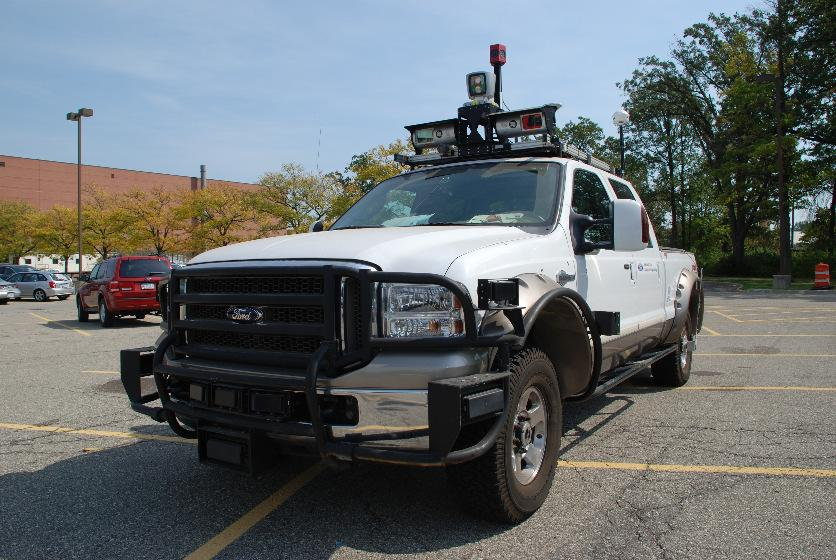
\includegraphics[width=0.5\textwidth]{img/sensor_fusion/ford_sensors.jpg}
	\caption[Ford 250 used to acquire Ford Campus dataset.]{Ford 250 pickup equipped with some sensors described in the Section~\ref{sec:introduction:scope_motivation}. On the top, the Ladybug omnidirectional camera, on the back the \ac{imu} and \ac{gps} unit.}
	\label{fig:sota:ford_sensors}
\end{figure}

The data is provided in raw format, accompanied by log files with timestamps, \ac{gps} and \ac{lcm}\footnote{For more information on \acf{lcm} protocol for estimating delays between sensory data registration on master-slave systems, see~\cite{Huang2010a}.} logs with all raw data. The images from an omnidirectional camera %, a Point Grey Ladybug3, 
are stored on \ac{ppm} and \ac{lidar} data %from a Velodyne HDL-64E
on \ac{pcap} format, from the \ac{tcp} connection socket.%; two Riegl LMS-Q120 \acp{lidar} also provide more information on the scan.

Rectified and synced data is stored in \ac{matlab} \textit{.mat} files. Along with the raw data and synced and rectified \textit{.mat} files, source code is also provided for parsing the raw data, visualizing the \ac{lcm} logs and pre-processed data on \ac{matlab}. Software that can render textured point clouds, implemented in C and \ac{opengl}, is also provided.


\subsection{\acl{kitti} Dataset}
A well known dataset for researchers of computer vision, autonomous driving and \ac{ml}, \ac{kitti} was recorded in 2011 and released to the public in 2013. This dataset contains various driving scenarios: suburban, highways, residential and campus areas; with trucks, cars, cyclists and persons. Alongside with data for testing, calibration measures are provided for all sensors.

The test car, a Volkswagen Passat, is equipped with two stereo pairs, one with color and one with gray cameras, a \ac{lidar}, an \ac{imu} and a \ac{gps} sensor, is shown in Figure~\ref{fig:sota:kitti_sensors}. Data from all four cameras is stored on \ac{png} format, \ac{lidar} measurements stored as a binary float matrix, and \ac{gps} and \ac{imu} are saved textually. Additionally, the raw data logs containing the timestamps and the transformations between the sensors are also provided. Labeled data is also available for some test scenarios in \ac{xml} files.

\begin{figure}[!ht]
	\centering
	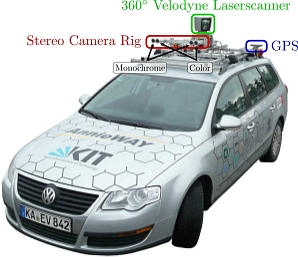
\includegraphics[width=0.5\textwidth]{img/sensor_fusion/passat_sensors.jpg}
	\caption[Volkswagen Passat used for recording \acs{kitti} dataset.]{Volkswagen Passat equipped with the sensors described in Section~\ref{sec:introduction:scope_motivation} graphs, for the \ac{kitti} dataset. On the top, the Velodyne \ac{lidar} and below the 2 stereo pairs (color and grey). On the back, the \ac{imu} and \ac{gps} systems are present.}
	\label{fig:sota:kitti_sensors}
\end{figure}


Along with the data and calibration parameters, several tools written in C++ or \ac{matlab} are also provided. The dataset offers two types of data categories: (1) unsynced and unrectified data or (2) synced and rectified data. The latter type is the one relevant for sensory calibration purposes.

The sensory apparatus contains 2 PointGray Flea2 greyscale and color cameras, a Velodyne HDL-64E \ac{lidar}~\cite{VelodyneHDL64}, among others less relevant sensors~\cite{Geiger2013a}.

\subsection{Udacity Self-Driving Car Nanodegree Dataset}
The data from Udacity online course on self-driving car is also publicly available~\cite{udacity}. This dataset dates to 2016 and was gathered to develop level 4 autonomy vehicles, containing much more data diversity than the previous two. The data available contains images from 3 color cameras,  \ac{lidar}, \ac{imu} and \ac{gps}, among other sensory data, such as speed, braking, etc.

This information is not available in raw format, only structured in \ac{ros} \textit{.bag} files. Some tools for visualizing and interacting with their data are provided for \ac{ros}~\cite{udacity}. 

Not much information about the sensors and their positioning is publicly available, and the dataset does not contain information for calibration.

\subsection{Summary}
Table~\ref{tab:sota:datasets_comparison} summarizes all the relevant data from the datasets~\cite{udacity, Pandey2011, Geiger2013a}. While there are few differences between the relevant types of data gathered, major differences can be observed on the format in which they are provided. 

The diversity of scenarios and size of the dataset is also an important aspect to consider. On this matter, \ac{kitti} and Udacity's are superior to Ford dataset, with \ac{kitti} providing the largest dataset in quantity, with already rectified and synced data. 
	
\begin{table}[!ht]
	 %\rowcolors{4}{gray!10}{white}
	 \renewcommand{\arraystretch}{1.2}
	 \centering
	 \begin{tabular}{@{}llccc@{}}
		 \toprule
		 \multicolumn{2}{l}{\multirow{2}{*}{Characteristics}} & \multicolumn{3}{c}{Datasets} \\ \cline{3-5}
																& & Ford Campus  & \acs{kitti} & Udacity \\ \midrule
																%
		 \multicolumn{2}{l}{\textit{Sensors and Data}} \\   \rowcolor{white}
		 \phantom{a}								& \ac{lidar}	   & \checkmark  & \checkmark & \checkmark \\ \rowcolor{gray!10}
																& Color Camera	 & \checkmark  & \checkmark & \checkmark  \\ \rowcolor{white}
																& Grey Cameras   &             & \checkmark &  \\ \rowcolor{gray!10}
																& Stereo Camera  &             & \checkmark & \checkmark  \\ \rowcolor{white}
																& Omnidirectional Camera &  \checkmark  &  &  \\ \rowcolor{gray!10}
																& \acs{imu}      & \checkmark  & \checkmark & \checkmark  \\ \rowcolor{white}
																& \acs{gps}      & \checkmark  & \checkmark & \checkmark  \\ \rowcolor{gray!10}
																& Driving data\footnotemark & & & \checkmark \\ \midrule \rowcolor{white}
		 \multicolumn{2}{l}{\textit{Data Formats and Tools}}  \\
		 \phantom{a}											 & Raw data available & \checkmark & \checkmark &  \\ \rowcolor{gray!10}
																			 & Data parsing tools & \checkmark & \checkmark & \checkmark  \\ \rowcolor{white}
																			 & Rectified data & \checkmark & \checkmark & \checkmark \\ \rowcolor{gray!10}
																			 & Synced data & \checkmark & \checkmark &  \checkmark  \\  \rowcolor{white}
																			 & Calibration parameters & \checkmark  & \checkmark  & \\ 
	   \bottomrule
		 \multicolumn{2}{l}{Raw data for sensors calibration} & \checkmark & \checkmark & \\ \rowcolor{gray!10}
		\multicolumn{2}{l}{\ac{ros} data compatibility} &  & \checkmark\footnotemark & \checkmark \\
		\multicolumn{2}{l}{Date of acquisition} & 2009  & 2011 & 2016 \\
		\bottomrule
	\end{tabular}
	\caption[Comparative analysis between the datasets.]{Comparison between the datasets more appropriated to this thesis objectives.}
\label{tab:sota:datasets_comparison}
\end{table}
\addtocounter{footnote}{-1}
\footnotetext{Other driving data includes, but it is not limited to: vehicle speed, joints states, twist, brakes, suspension, fuel level, \ac{can} bus data, steering, tire pressure, among many others.}
\addtocounter{footnote}{1}
\footnotetext{While Udacity dataset is the newest and provides direct out-off-the-shelf integration with \ac{ros}, that type of integration can also be achieved for \ac{kitti} by using other tools, such as \textit{kitti2bag}~\cite{TomasKrejci}.}

Comparing the 3 datasets using the information in Table~\ref{tab:sota:datasets_comparison} and the previous sections, Udacity and \ac{kitti} are better suited to the purposes of this work. They provide a larger dataset than Ford, have \ac{ros} compatibility and the tools provided are open-source and not developed to be used on proprietary software.

Since Udacity dataset integrates more easily with \ac{ros} than \ac{kitti}, providing also some tools for \ac{ros} preliminary tests, learning and earlier development stages were based on this dataset. Later, due to the lack of calibration parameters and raw data for sensors calibration\footnote{Note that, despite the Udacity dataset not providing data to ease the calibration of its sensors, such as camera intrinsic calibration or the extrinsic calibration between \ac{lidar} and camera, such calibration parameters can be obtained from this data. Those parameters are not as accurate as those obtained using a proper calibration setup and are out the scope of this work (being another research topic on itself) and therefore no effort will be dedicated to this topic.}, \ac{kitti} dataset was used instead.


%%%%%%%%%%%%%%%%%%%%%%%%%%%%%%%%%%%%%%%%%% CAMERA %%%%%%%%%%%%%%%%%%%%%%%%%%%%%%%%%%%%%%%%%%

\section{Camera as a sensor on \acl{cv} applications}
\label{sec:sota:camera}
Vision is the human sense most relevant to how we perceive the world and how we navigate in it~\cite{Ekstrom2015, Beck1983}. Replicating this ability on machines, through the usage of cameras, is a widely researched topic on computer vision and instrumentation~\cite{Beck1983}. The most common cameras, as our eyes, take advantage of the pinhole effect: a small hole (or pin), that is used to spatially filter the non-focused light beams through an aperture or lens~\cite{Beck1983, camera_models, Sturm2010}, producing a mirrored, but focused image.

On the following sub sections, basic notions of the current status of camera models and camera calibration are given. Since this research is focused strictly to the application of a camera as a sensor on computer vision, the overview provided abstains from describing extensive research on camera technologies and camera models for the field of computer vision. From a purely working principle and technologies, several camera types can be named, such as catadioptric, plenoptic, biprism, among others~\cite{Sturm2010}. %Considering consumer market, denominations such as Compact Cameras, \ac{dslr} cameras, Mirrorless (or \ac{evil} cameras) can also be used~\cite{comercial_cameras}. 
For further research, the reader might be interested on~\cite{comercial_cameras, Sturm2010, camera_models, Merklinger1993, Photopillers}.


\subsection{Camera Geometry}
\label{subsec:sota:camera-geometry}
A world point in a 3-dimensional Euclidean space can be represented by a vector with 3 real coordinates: $(X, Y, Z)$ and an image pixel of a digital image is typically represented as an element of a 2D matrix with integer coordinates $(u, v)$~\cite{mvg_book}. From a mathematical standpoint, a camera can be considered as a mapping tool between the world objects in three dimensions into a 2D image plan, such as depicted by Equation~\eqref{eq:camera_transform}, which leads to different mathematical models used to describe the camera~\cite{mvg_book, Sturm2010}.

\begin{equation}
	\label{eq:camera_transform}
	(X, Y, Z) \xrightarrow[]{\text{transformation}} (u, v)
\end{equation}

When describing camera models, several considerations should be made~\cite{Sturm2010}:
\begin{itemize}
	\item \textbf{Central Camera Models vs Non-Central Camera Models}: quantifies the number of optical centers on a camera. A central camera has only one optical center through which all light rays pass through to reach the film and a non-central has two or more optical centers;
	\item \textbf{Global vs Local models:} indicates if the parameters of the model are the same for all the image/\ac{fov} of the camera or if different regions of the image have different parameters, respectively.
\end{itemize}

For the application currently envisioned, global central camera models are considered. For a more detailed explanation of the topics above or an extensive overview of non-classical camera models, different types of projections and other aspects of modelling cameras, see~\cite{Sturm2010, camera_models}.

\subsubsection{Pinhole Camera Model}
Based on the pinhole effect, represented in Figure~\ref{fig:pinhole_effect}, the pinhole camera model is the most common camera model~\cite{camera_models}. The pinhole effect consists on using a small hole (or aperture) to spatially filter the light rays by angle of incidence, reducing the amount of light rays overlapping when coming from different incident angles through the pinhole, which otherwise would ``blur'' the image. 

\begin{figure}[!ht]
	\centering
	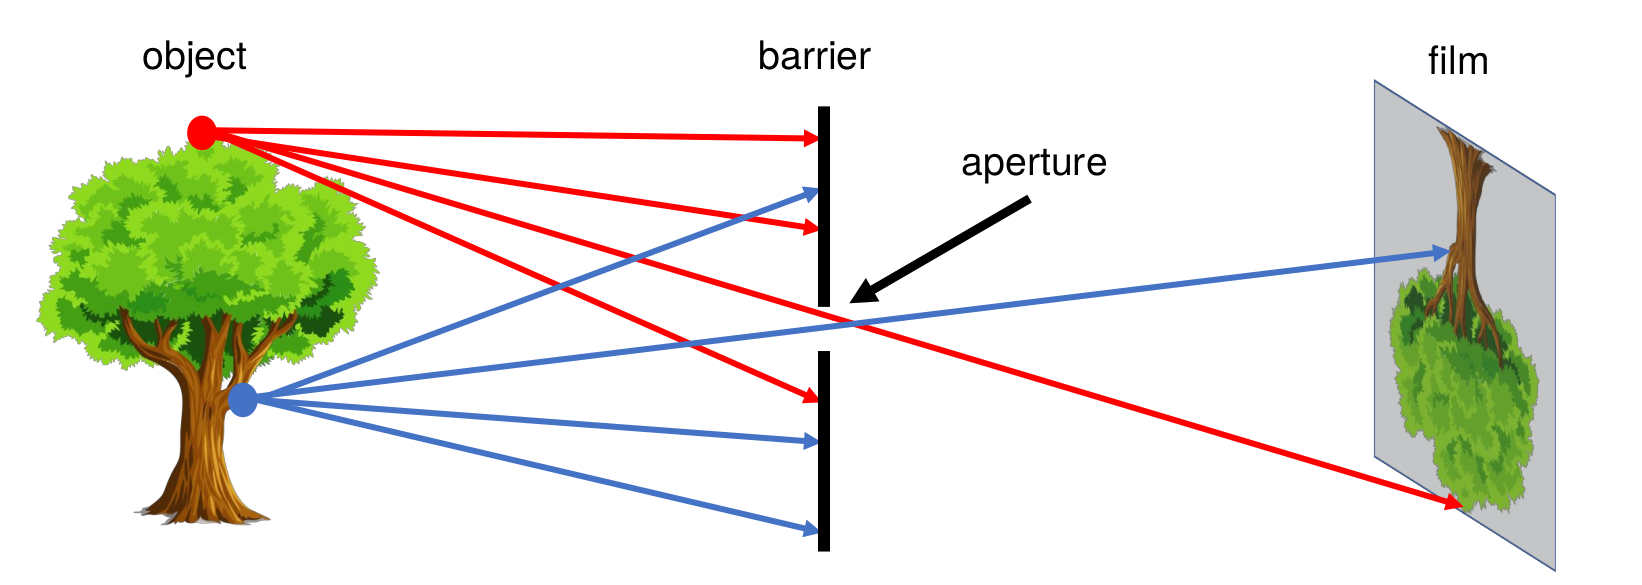
\includegraphics[width=0.6\textwidth]{img/camera/pnhole_effect.png}
	\caption[Pinhole effect on a small aperture.]{Pinhole effect on a small aperture. Source:~\cite{camera_models}.}
	\label{fig:pinhole_effect}
\end{figure}

The pinhole camera model describes the perspective transformation on Equation~\eqref{eq:camera_transform} as a central projection where all light rays meet at the camera center, $\mathcal{F}_c$. A diagram of the pinhole camera is shown in Figure~\ref{fig:pinhole_camera_model}. 

On this model, the z-axis is collinear with the optical axis\footnote{Also called principal axis. The two terms can be interchanged with no loss of context.}, aligned with the direction the camera is facing. The image plane is at $z = f$, where $f$ is the focal length, being intersected by the optical axis on the principal point, with coordinates $(c_x, c_y)$ on the image plane axis. Note that the principal point is not the origin of the referential on the image plane, but instead the middle point, being the origin located in the top left corner, with a downward y-axis.

\begin{figure}[!ht]
	\centering
	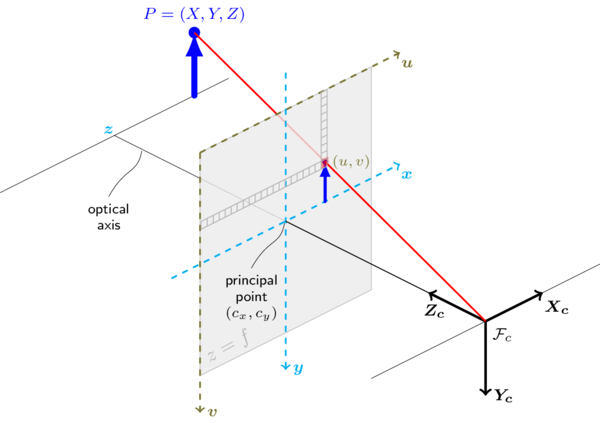
\includegraphics[width=0.6\textwidth]{img/camera/pinhole_camera_model.png}
	\caption[Pinhole camera model.]{Pinhole camera model. Source:~\cite{opencv_doc}}
	\label{fig:pinhole_camera_model}
\end{figure}

Due to the nature of the pinhole camera model, it is more convenient to use a Projective Space instead of the more common Euclidean Space~\cite{mvg_book, camera_models, Sturm2010}. On a Projective Space, as in a central camera model, all of its points are oriented through a single point~\cite{mvg_book}. Therefore, by using a projective space instead of a Euclidean for addressing the transformations of a pinhole camera model, becomes more intuitive and relatable to the actual geometry of the model. Despite projective spaces using homogeneous coordinates and non-Euclidean geometry, homogeneous coordinates can be converted for cartesian coordinates without loss, if the homogeneous points are possible to represent on a Euclidean coordinate frame~\cite{mvg_book, camera_models}.

\subsubsection{Projective Geometry}
A tridimensional Euclidean Space can be represented on a Projective Space using 4 coefficients. Therefore, the previous tridimensional vector can be rewritten in homogeneous coordinates as $(wX, wY, wZ, w)$~\cite{mvg_book}. If $w \neq 0$, we can transform from the Projective to Euclidean Space, obtaining the world representation of such points by dividing the homogeneous point by $w$. For the cases in which $w =  0$, we have purely projective points at infinity, that only exist in Projective Space~\cite{mvg_book}. 

The relation depicted in Equation~\eqref{eq:camera_transform} can be expressed in projective geometry as in Equation~\ref{eq:projective-geometry-pixel}, where $P$ represents the projection matrix that performs the transform from world points to image pixels. 

\begin{equation}
	\label{eq:projective-geometry-pixel}
	\begin{bmatrix}
		u \\ v \\ 1
	\end{bmatrix}
= P \times 
\begin{bmatrix}
		X \\ Y \\ Z \\ 1
\end{bmatrix}, \qquad \text{if } w = 1.
\end{equation}

The projection matrix in a pinhole camera model is the result of multiplication of two matrices: the camera matrix (or matrix of the camera's intrinsic parameters), $K$; and a joint rotation and translation matrix, $[R|t]$, where $R$ is the rotation matrix and $t$ the translation vector. The combination of these matrices is given on Equation~\eqref{eq:projective_matrix} and the full camera transform is expanded on Equation~\eqref{eq:camera_transform_full}, through the replacement of Equation~\eqref{eq:projective_matrix} in Equation~\eqref{eq:camera_transform}.

\begin{equation}
	\label{eq:projective_matrix}
	P = K[R|t]
\end{equation}

\begin{equation}
	\label{eq:camera_transform_full}
	\begin{bmatrix}
		u \\
		v \\
		1
	\end{bmatrix}
	= 
	\overbrace{
		\underbrace{
			\begin{bmatrix}
				f_x & 0 & c_x \\
				0 & f_y & c_y \\
				0 & 0 & 1 
			\end{bmatrix}
		}_\text{\large\textbf{K}}
		\underbrace{
			\left[
				\begin{array}{ccc|c}
					r_{xx} & r_{yx} & r_{zx} & t_x \\
					r_{xy} & r_{yy} & r_{zy} & t_y \\
					r_{xz} & r_{yz} & r_{zz} & t_z 
				\end{array}
		\right]
		}_\text{\large\textbf{[R|t]}}
	}^\text{\large\textbf{P}}
	\begin{bmatrix}
		X \\
		Y \\
		Z \\
		1
	\end{bmatrix}
\end{equation}

The matrix of intrinsic parameters is used to represent the calibration parameters of the camera: the focal lengths of each axis, $f_x$ and $f_y$, which scale the $x$ and $y$ axis; the principal point offset to the axis origin, $c_x$ and $c_y$, for the x and y-axis, respectively, that translate the image center with relation to the origin of the camera referential. 

The joint rotational-translation matrix, $[R|t]$, is also known as the extrinsic camera parameters, translates the coordinates of a point to the Cartesian coordinate system fixed to the camera.


\subsubsection{Cameras, Lenses and Distortion}
Using a simple pinhole for filtering light rays 
%, that would blur the image severely, 
reduces the amount of light reaching the camera sensor. Therefore, a lens is used to collect the light and focus it onto the image plane, providing the same effects as the hole~\cite{Sturm2010}, while allowing more light to be captured. The paraxial refraction model is represented in Figure~\ref{fig:pinhole_with_lense}, from which we can consider the Pinhole Camera model by letting $z_0 = 0$, which implies $z' = f$ and the image is formed on the focal point.

%pinhole effect with a lens is depicted 

\begin{figure}[!ht]
	\centering
	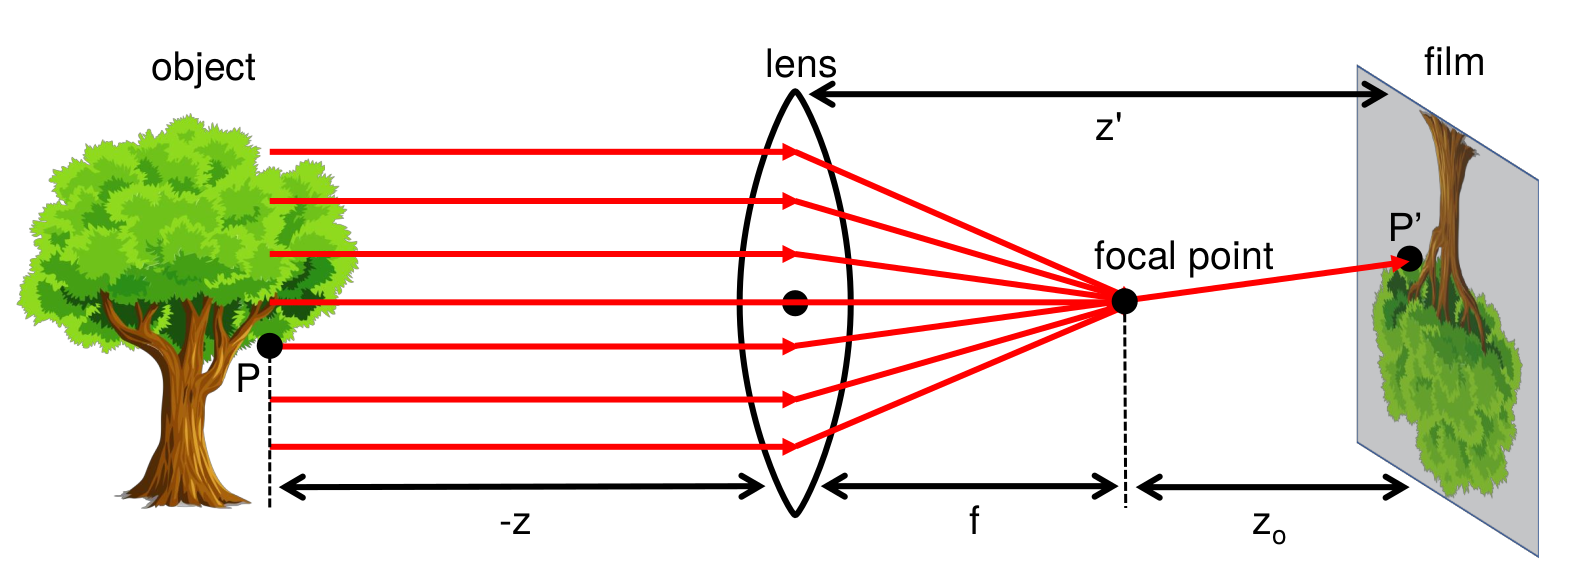
\includegraphics[width=0.6\textwidth]{img/camera/pinhole_with_lense.png}
	\caption[Pinhole effect on a lens]{Pinhole effect on a lens. Source:~\cite{camera_models}}
	\label{fig:pinhole_with_lense}
\end{figure}

Since lenses introduce non-linear distortion, the pinhole camera model needs to be extended to included radial and tangential distortion parameters~\cite{Bouguet2010, manuapphotogrammetry, Heikkila1997}. Such parameters indicate how the non-linear distortion of the camera lenses affects the image projection on the camera plane~\cite{camera_models, Sturm2010} and how can this be corrected~\cite{Heikkila1997, Bouguet2010, opencv_doc}. The equations behind that expression are beyond the scope of this introduction and therefore will not be detailed here, but the effect of lens aberration can be seen in Figure~\ref{fig:lense_distortion_types}.

\begin{figure}[!ht]
	\begin{subfigure}[c]{0.3\textwidth}
		\centering
		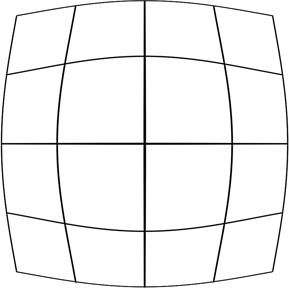
\includegraphics[width=0.6\textwidth]{img/camera/distortion-barrel.png}
		\caption{}
		\label{fig:barrel-distortion}
	\end{subfigure}
	%\quad 
	\begin{subfigure}[c]{0.3\textwidth}
		\centering
		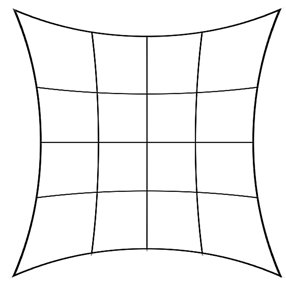
\includegraphics[width=0.6\textwidth]{img/camera/distortion-pincushion.png}
		\caption{}
		\label{fig:pincushion-distortion}
	\end{subfigure}
	%\quad
	\centering
	\begin{subfigure}[c]{0.3\textwidth}
		\centering
		
\includegraphics[width=0.6\textwidth]{img/camera/no-distortion.png}
		\caption{}
		\label{fig:no-distortion-lens}
	\end{subfigure}

	\caption[Effects of barrel and pincushion distortion caused by a non-linear klens.]{Barrel~(\subref{fig:barrel-distortion}) and Pincushion~(\subref{fig:pincushion-distortion}) distortion caused by the non-linear behavior of the camera lens. The effect of an ideal lens, with no distortion, is shown on~(\subref{fig:no-distortion-lens}). Source:~\cite{camera_models}.}
	\label{fig:lense_distortion_types}
\end{figure}

For more information on the pinhole camera model and lens distortion, see Hartley and Zisserman Multi View Geometry in Computer Vision~\cite{mvg_book}, Hata and Savarese course notes~\cite{camera_models} or \acf{opencv} official documentation~\cite{opencv_doc}. 

\subsection{Camera Intrinsic Calibration}
\label{subsec:sota:camera-intrinisc-calibration}
Calibrating a camera is the process in which the parameters of the model that describes its behavior are determined. For the extended pinhole camera model, this means determining the parameters of its intrinsic matrix, $K$, but also the distortion coefficients of the lens used~\cite{mvg_book, camera_models, Bouguet2010, Heikkila1997}. These parameters are called the intrinsic parameters and are independent of the scenario being viewed, if the focal length is kept constant. On the other hand, extrinsic camera parameters are different for every situation and therefore scenario dependent~\cite{opencv_doc, Bouguet2010, Heikkila1997}.

Zhang proposed in 2000 a method for calibrating a camera that unlike previous work, does not require a special setup, expensive experimental apparatus or complicated calibration patterns: it uses a planar object with a known pattern, which can be freely moved in front of the camera~\cite{Zhang2000}. Only two images are necessary for camera calibration, as long as the pattern movement between them is not a pure translation. The estimation of the camera intrinsic parameters and distortion caused by the lenses can be determined by solving Equation~\eqref{eq:camera_transform_full}, once several $2D \leftrightarrow 3D$ correspondences have been established.

Zhang's algorithm differs from other algorithms at the time that attempted to calibrate a camera by rotating it on a static environment. Other alternatives include Tsai's algorithm~\cite{Roger1987, mvg_book}, a 2-stage technique for camera calibration first presented in 1987, that does not determine the camera center. A \ac{dlt} algorithm can also be used to determine the camera calibration parameters (see~\cite{mvg_book}).

Following Zhang's algorithm, the correspondences between the 2D and 3D representations of the pattern can be made by finding the corners or circles on planar patterns~\cite{opencv, mvg_book}. Chessboards are the most common patterns used today~\cite{opencv}, allowing corner detection for each cell (Figure~\ref{fig:opencv_calib_pattern}). Since the dimensions of the cell and their arrangement are known previously, it is possible to compute the orientation of the chessboard~\cite{Zhang2000, opencv_doc, mvg_book}. On those conditions, revisiting Equation~\eqref{eq:camera_transform_full}, only the $K$ matrix is left to be determined. 

\begin{figure}[!ht]
	\centering
	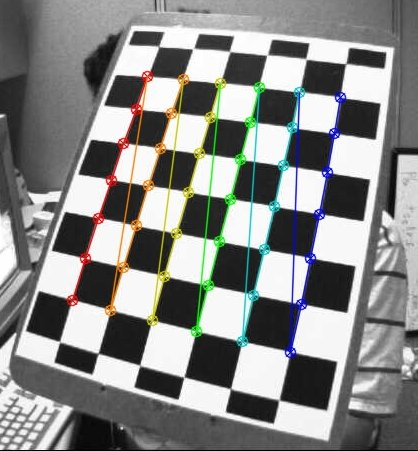
\includegraphics[width=0.4\textwidth, keepaspectratio]{img/camera/calib_pattern.jpg}
	\caption[Chessboard calibration pattern with the corners used for calibration.]{Chessboard calibration pattern with the detected corners overlapped. Source:~\cite{OpenCV_camera_calib}.}
	\label{fig:opencv_calib_pattern}
\end{figure}

The intrinsic calibration matrix coefficients can then be refined using a maximum-likelihood estimation to minimize the error using a non-linear method, such as Levenberg-Marquardt optimization~\cite{Levenberg1943}. Other optimizations are possible, such as Powell’ dog-leg non-linear least squares technique~\cite{Lourakis2005}. Further reading can be conducted on~\cite{mvg_book, Sturm2010, camera_models, Hata, Xu1996a}.

Bouguet in 2010 provided a Camera Calibration toolbox for \ac{matlab}~\cite{Bouguet2010}, which serves as the basis for many camera calibration toolboxes nowadays, such as \ac{opencv}, which is also based on the work of Zhang~\cite{opencv}.

\subsection{Image Processing Libraries for \acl{cv}}
In the field of computer vision, several tools and libraries are available, capable of performing low image operations, image detection, filtering, among others. This sub-section will list and briefly describe these tools.

\begin{itemize}
	\item \textbf{BoofCV~\cite{boofcv}:} written in Java, this library is oriented to real-time image operations, such as low-level image processing, camera calibration and feature/object  detection, tracking and recognition;
	\item \textbf{Dlib~\cite{dlib}:} modern C++ toolkit containing \acl{ml} algorithms and tools, some on the field of computer vision;
	\item \textbf{\ac{matlab} Computer Vision Toolbox\texttrademark~\cite{matlabcvtoolbox}:} toolbox for computer vision algorithms, 3D vision, and video processing systems. Can perform object detection and tracking. Detects, extracts and matches features;
	\item \textbf{\acf{opencv}~\cite{opencv}:} open source library for C++, Python and C that implements the state of the art algorithms on computer vision;
	\item \textbf{Vlfeat~\cite{vlfeat}:} open source library for C that implements many state of the art algorithms on computer vision;
	\item \textbf{SimpleCV~\cite{simplecv}:} Open source framework, written in Python, that can be used to implement computer vision software using other libraries;
\end{itemize}

Since a goal of this work is to use Open-Source tools as far as possible (instead of using closed source tools or code that is harder to integrate with other libraries), which is common among the automotive industry on the field of autonomous vehicles, \ac{matlab} \acl{cv} Toolbox\texttrademark~does not suit. The code of this work is mainly developed in C++, so Python and Java libraries will not be considered, resulting only in \ac{opencv} and Dlib, since Vlfeat uses plain C. 

\ac{opencv} has a large and active community and is considered by many researchers and industry leaders as the \textit{de facto standard} library regarding computer vision. Dlib is a robust library, but no significant differences can be seen when comparing with \ac{opencv}. Therefore, the final choice for a computer vision library is \ac{opencv}, also because of the already implemented compatibility with \ac{ros}.



%%%%%%%%%%%%%%%%%%%%%%%%%%%%%%%%%%%%%%%%%%% LIDAR %%%%%%%%%%%%%%%%%%%%%%%%%%%%%%%%%%%%%%%%%%

\section{Automotive \ac{lidar}}
\label{sec:sota:automotive-lidar}
\ac{lidar} sensors map their surroundings thanks to their high spatial resolution and capability of precisely measuring depth. Already used in topography, spectrography and air pollution studies, \ac{lidar} found its importance on the automotive industry as one of the key sensors of autonomous cars and \ac{adas}~\cite{Sullivan2016}. 

The maps produced by \ac{lidar}, commonly represented as point clouds or mesh clouds models (Figure~\ref{fig:bunny}), are one of the preferred method for \ac{slam} algorithms, which allow a vehicle without previous knowledge of its surroundings to autonomously navigate them, a crucial task for \ac{adas} on self-driving vehicles.

Point clouds represent the spatial data measured by the \ac{lidar} as points on the tridimensional space. The objects represented on a point cloud are formless, as they have no relation with their ``adjacent'' points, as depicted in sub-Figure~\ref{fig:bunnyPointCloud}. A Mesh cloud representation of the point cloud in sub-Figure~\ref{fig:bunnyMeshCloud}, produced from by the point cloud in sub-Figure~\ref{fig:bunnyPointCloud}, is a representation of the same points united by lines, forming a mesh. A mesh cloud conveys form, as can be verified by comparing the point cloud with the mesh representation of the same data. A mesh cloud, contrary to a point cloud, can also represent a close form and therefore having a volume.

\begin{figure}[!ht]
	\centering
	\begin{subfigure}[c]{0.45\textwidth}
	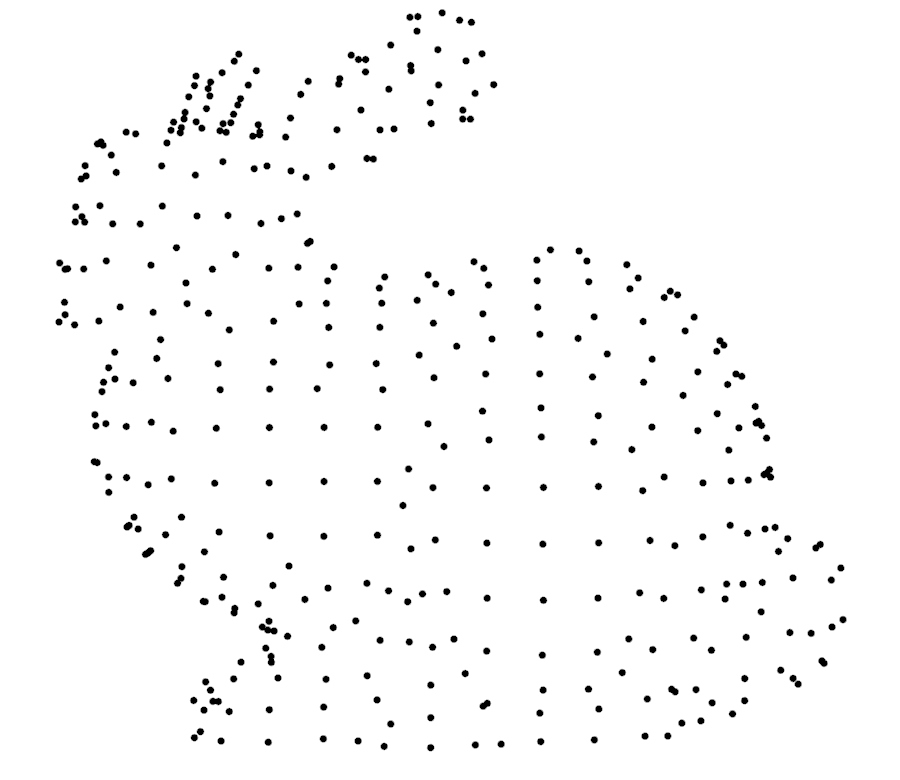
\includegraphics[width=\textwidth]{img/lidar/bunny_point.png}
		\caption{Point Cloud representation}
		\label{fig:bunnyPointCloud}
	\end{subfigure}
	\quad
	\begin{subfigure}[c]{0.4\textwidth}
		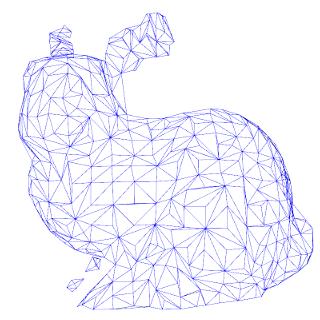
\includegraphics[width=\textwidth]{img/lidar/bunny_mesh.png}
		\caption{Mesh Cloud representation}
		\label{fig:bunnyMeshCloud}
	\end{subfigure}
	\caption[Example of a point and mesh clouds.]{Stanford bunny~\cite{bunny} point cloud (\subref{fig:bunnyPointCloud}) and mesh cloud (\subref{fig:bunnyMeshCloud})}
	\label{fig:bunny}
\end{figure}

\subsection{\ac{lidar} classification based on the depth measurement principle}
Regarding the type of signals and principles for measuring the scene distance, \acp{lidar} can be either \ac{cw} (emit a sinusoidal or square modulated signal), pulsed (emit a square pulse at fixed moments in time)~\cite{Payne2009, TexasLiDAR, SpringerOptics} or other more exotic and experimental types, that will not be addressed here, since they are out of the scope of this work.

\ac{cw} \acp{lidar} continuously emit a modulated \ac{laser} signal to their surroundings and, depending on the modulation technique, this signal can either be \ac{am} or \ac{fm}\cite{TexasLiDAR}. \ac{am}\ac{cw} \acp{lidar} operates by emitting a pseudo-random stream of binary data and coherently detecting the received signal. The phase shift distance, measured between the emitted and received signal, is directly related with the distance at which the pulse was reflected.

If \ac{fm}\ac{cw} is used instead, the \ac{lidar} \ac{laser} sends a frequency chirp\footnote{A signal whose frequency varies linearly with time.} and coherently detects the received signal, estimating the distance at which the reflection occurred (i.e., the distance at which the object is), by the frequency shift between the emitted and reflected signals~\cite{Payne2009, TexasLiDAR}. Coherent detection can be performed by heterodyne or homodyne detection, but such details will not be addressed here. A brief description and comparison between the two detection modes applied to \ac{lidar} technology is given in~\cite{Conroy2009}, and the underlying theory can be consulted on~\cite{Carlson2010, SpringerOptics}.

Pulsed \ac{lidar} technology acquires depth information by measuring the \acf{tof} between the reflection and emission of the same light pulse by the \ac{lidar} \ac{laser}. This technology is the most common type used for measuring depth on automotive \ac{lidar}~\cite{Sullivan2016}, and therefore this work will be based on pulsed~\ac{tof} technology to measure the distance at which the obstacles on the scene are present.

Both \ac{cw} and \ac{tof} \ac{lidar} have advantages and disadvantages, but they will not be compared here. Further reading about the topic can be found on~\cite{Sullivan2016, Simonite2017, Payne2009, TexasLiDAR}.


\subsection{\ac{lidar} classification based on construction}
Despite the depth measurement technique used by \ac{lidar} devices, regarding its construction and mapping technology, automotive \acp{lidar} can be one of the following categories~\cite{Hecht2018, Sullivan2016}:

\begin{enumerate}
	\item \textbf{Rotating \ac{lidar} or Macro-scanners:} the most common type, the \ac{lidar} optical and electrical circuit are mounted on a mechanical rotating device, which normally results on a wider \ac{fov} than the other models~\cite{Sullivan2016};
	\item \textbf{Flash:} organized in a matrix structure, similar to a standard \ac{ccd} or a \ac{cmos} camera, every element of the matrix contains a photodetector. A ``flash'' simultaneous illuminates all the \ac{fov}, and the reflected light intensity and time of arrival is measured to provide depth calculations, simultaneously for all pixels of the depth image~\cite{TetraVue, Ouster, Gelbart2002,Stettner2010, Simpson2019}; 
	\item \textbf{\ac{mems}:} operate by controlling the angle at which a rotating microscopic mirror is aligned with the \ac{laser}. By varying the angle, a single line can be scanned and using multiple \acp{laser} with the same mirror allows vertical scan~\cite{LeddarTech, Yoo2018};
	\item \textbf{Phased Arrays:} still on an embryonic stage, phased array \ac{lidar} use a microscopic array of antennas, similar to a \ac{radar}, where the phase of each antenna is individually controlled to allow the \ac{lidar} to sweep and/or focus on a specific area, using beamforming theory~\cite{Quanergy2018, Yu2016}.
\end{enumerate}

Of all the four types of \ac{lidar} presented, \ac{mems} and phased array \ac{lidar} are still unsuited for autonomous vehicles, since they have yet to leave their early research state and develop a functional prototype~\cite{Sullivan2016, Hecht2018}. 

Flash \acp{lidar}, also referred by some authors as solid state \ac{lidar}, since it has no movable parts, has the potential to become the most reliable, durable and cheaper \ac{lidar} technology~\cite{Sullivan2016, Hecht2018, Fersch2017a}. However, this technology is not yet mature, with some of its best experimental  prototypes achieving a maximum distance of \SI{2}{\meter}~\cite{Hecht2018}. The main cause for such lower range is the attenuation of the flash intensity, since its power is inversely proportional to the squared distance and the power the can endure.

Some prototypes are also unveiled from startups, such as TetraVue~\cite{TetraVue} and Ouster~\cite{Ouster}, and some patents are being registered~\cite{Simpson2019}; but this \ac{lidar} technology is not yet suited for the automotive market of autonomous cars~\cite{Fersch2017a}.

Therefore, only one alternative remains: a mechanical rotating \ac{lidar}, which is the technology that will be chosen for this work.

\subsection{The Mechanical Rotating \ac{lidar}}
To construct a rotating \ac{lidar}, a single pair of \acp{laser} and photodetectors are assembled on a fast rotational device (typically \SIrange{5}{20}{\revspersecond}), allowing that pair to scan a single line while rotating, creating a 2D \ac{lidar}. If multiple pairs are assembled with different polar angles, the \ac{lidar} is said to be a 3D \ac{lidar}, since a total revolution can produce a three-dimensional map of its surroundings~\cite{Sullivan2016}.

While a rotating \ac{lidar} consumes more power than the other counterparts, it can also achieve ranges until 100 meters~\cite{vlp16, Sullivan2016} or even 200 meters~\cite{VelodyneHDL64, Pandar40UserGuide, Sullivan2016}. To measure the depth on a rotational \ac{lidar}, \ac{tof} is the most common technique, being the pulse triggered at a defined angular step when rotating.

Regarding rotating \acp{lidar} technology, only 5 relevant companies exist worldwide. Velodyne\cp~\cite{Velodyne}, HESAI\cp~\cite{Hesai}, RoboSense\cp~\cite{Robosense}, Ouster\cp~\cite{Ouster} and Quanergy\cp~\cite{Quanergy}. Velodyne is the undisputed market leader~\cite{Sullivan2016, Hecht2018}, with several rotating \ac{lidar} solutions, ranging from \SIrange{16}{128}{} \ac{laser} beams.

Quanergy is a \ac{lidar} company that is focused on bringing solid state \ac{lidar} to the market. They provide one mechanical rotation \ac{lidar} solution, but with only 8 beams, which is not suited for the demands of autonomous driving~\cite{Sullivan2016, Hecht2018}. 

Ouster is a startup that produces mechanical rotational \acp{lidar}. They have two models, \texttt{OS-1} and \texttt{OS-2}, for mid and large range, respectively, which differ on their \ac{fov}, range and number of beams~\cite{Ouster}.

HESAI and RoboSense are two Chinese \ac{lidar} manufacturers whose products are similar to Velodyne's. In fact, they are so similar that a lawsuit as been filled against them by Velodyne, for intellectual property issues~\cite{VelodyneLawsuit}. This lawsuit is due to Velodyne holding the patent on mechanical rotating \acp{lidar} with surround view\cite{Hall2011}, which ensures its dominance on the market of mechanical \acp{lidar}. 

In fact, on their specifications, \acp{lidar} from Velodyne, HESAI, RoboSense or Ouster differences are \ac{laser} position managing, range and vertical \ac{fov}. On the other hand, they severely differ in terms of prices, with top of the range Velodyne \ac{lidar} selling for $\$85000$ and the cheaper at some thousand dollars. 

For our work, since Velodyne's is the top of the market solution and the more mature, it makes sense to test \ac{lidar} interference on the most used solution, since if two \acp{lidar} will interfere on the road, the most likely scenario is that they are from Velodyne's.

\subsection{Point Cloud Processing Software}
Considering only point cloud software targeted to developers and not final users, VeloView\texttrademark, a \ac{lidar} data visualizer by Velodyne is excluded as an alternative for this thesis, since it only allows to visualize data and save/load data from files. Similarly, programs that only intend to provide some features to apply to point clouds, and do not allow for research on point cloud processing to be conducted, are not viable solutions for this work. 

From the software that has not being excluded by the previous conditions, several point cloud processing libraries were researched and are detailed below:

\begin{itemize}
	\item \textbf{\ac{cgal}:}	a library containing geometric algorithms, written in C++, optimized for polygons and polyhedra processing, whose target are geographic information systems, such as computer aided design, molecular biology and robotics, among others~\cite{CGAL};
	\item \textbf{\ac{pdal}:} written in C++, \ac{pdal} is an adaptation of \ac{cgal} optimized to handle point cloud data. It is more oriented for the user to define a process pipeline in JavaScript, from already available algorithms on its library than for the developer to implement its own~\cite{PDAL};
	\item \textbf{Open3D:} written in C++, Open3D is a library optimized for common operation in point cloud processing, providing voxelization, nearest neighbor search, normal estimation and visualization interfaces, among other utilities~\cite{Open3D};
	\item \textbf{\acf{pcl}:} Open-Source and with an active community, \ac{pcl} is a large library for 2D/3D image processing and point cloud processing. It allows generic data types, has a comprehensive amount of state of the art algorithms and easily integrates with \ac{opencv} and \ac{ros}~\cite{PCL}.
\end{itemize}

All the alternatives are written in C++, the programming language of choice for this work. From the 4 libraries, \ac{cgal} is not optimized for point cloud data and \ac{pdal} intends to simplify routine point cloud processing, which is not aligned with the objectives of this thesis; for this reason, they are both excluded. Open3D and \ac{pcl} are reasonable alternatives, but \ac{pcl} modularity (allowing the user to define its data types) and extent of already implemented algorithms makes it a better solution than Open3D. Since we will also use \ac{opencv} and \ac{ros}, which \ac{pcl} allows integration with and this topic is widely detailed on forums, our choice for a point cloud processing library is \ac{pcl}.

\section{Camera and \ac{lidar} Extrinsic Calibration}
\label{sec:sota:extrinsic_calibration}

On a multiple sensor setup, coordinated frames from one sensor must be able to be referred on another sensor coordinate frame. Transforming data from one frame to another requires performing extrinsic calibration between them by determining the rigid body transform that can convert the data from one reference plan to the other without loss of information.

Therefore, the sole purpose of extrinsic calibration is to determine the coefficients of this transform, that can be described as a rotation and a translation, similarly to the joint rotation-translation matrix $[R|t]$ used for camera intrinsic calibration (Equation~\eqref{eq:camera_transform_full}). However, on this case, instead of this matrix representing the rotation of the object to the camera or the camera movement in the world, it represents the rotation and translation operations that need to be applied to the coordinate system of one sensor (and its data) to align the data with the coordinate system of another sensor. The precision of this transformation takes particular interest when data fusion (or sensor fusion) is being achieved, i.e., merging from this data sources to reduce errors and improve the significance of data each sensor is capable of giving. 

Several algorithms have been suggested for performing extrinsic calibration on data. They range from the necessity of well controlled environments to requiring no human intervention, using or not a calibration pattern. 


\subsection{Calibration using Patterns}
Typical extrinsic calibration between \ac{lidar} and camera with intersecting \ac{fov} use calibration patterns: Unnikrishnan first proposed a \ac{lidar} to Camera extrinsic calibration using a toolbox developed to manually select correspondences between a calibration pattern on image and point cloud~\cite{Unnikrishnan2005}. A \ac{matlab} toolbox to ease the process was also developed in 2005 by Unnikrishnan\etal~\cite{Unnikrishnan}. Fremont\etal uses a planar calibration target with a hole surrounded by a solid color, matching the depth discontinuities from the \ac{lidar} with the color discontinuities from the camera~\cite{Fremont2013} and Velas uses a planar pattern with geometric objects carved on its surface~\cite{MartinVelas2013}. Liao\etal proposes a method that only requires the usage of a planar polygon of known shape~\cite{Liao2019} and Park\etal tests and presents results of this calibration method applied to multiple polygons, specially with triangular shape~\cite{Park2014}. Mirzaei\etal uses a planar pattern with fiducial marker~\cite{Mirzaei2012}. 

Regarding calibration with three-dimensional calibration targets, Pusztai uses a box with different colors on each face~\cite{Pusztai2018}; Pereira uses a ball (for performing multiple sensor calibration, instead of only 3D \ac{lidar} and monocular camera)~\cite{Pereira2016}; Gong a trihedral object, determining the extrinsic calibration parameters using a nonlinear least squares algorithm~\cite{Gong2013}.

While the previous methods were focused on calibrating monocular cameras with tridimensional \ac{lidar}, alternative methods exist for stereo systems, taking advantage of the disparity map obtained with a stereo camera. Automatic methods are proposed by Geiger\etal and Guindel \etal. Geiger\footnote{One of the researchers behind \ac{kitti}.} and Moosmann propose a method for calibrating such setup with a single shot, using chessboards with multiple sizes and orientations. Their algorithm initializes seed point on the chessboard corners on image, and by region growing algorithms detects the chessboard position on camera, while on \ac{lidar}, planar detection and successive refinement is applied~\cite{Geiger2012a}. Guindel\etal use a planar calibration target with four holes that can be detected on the stereo map from the camera and \ac{lidar} point cloud, extrinsically calibrating both sensors by detecting the holes center and compute the rotation and translation that minimizes error. 

\subsection{Calibration without human intervention or patterns}
Some automatic methods that do not require human intervention neither calibration patterns have also been present on the literature. Bileschi's method estimates all intrinsic camera parameters  (including radial distortion) and the rotation and translation between a camera and \ac{lidar}, that is later refined by discontinuity association~\cite{Bileschi2009}. Naroditsky \etal proposes an automatic calibration method using the multi-polynomial Macaulay resultant, that, paired with \ac{ransac} and least-squares refinement, can automatically calibrate the camera-\ac{lidar} setup~\cite{Naroditsky2011}. Shaukat proposes a solution for planetary space robots based on  stereopsis and depth maps matching using mesh grids stecthing~\cite{Shaukat2016}. Ishikawa \etal calibration method, computes the calibration parameters using two main steps: first, it initializes the parameters from the movement of the camera and \ac{lidar} and secondly, refines those parameters using sensor-fusion until convergence~\cite{Ishikawa2018}. 

Jeong \etal presents a framework for calibrating \ac{lidar} and stereo cameras with non-overlapping \ac{fov}, by utilizing road markings and robust optimization algorithms and cost functions~\cite{Jeong2019}.

Using mutual information techniques, Taylor and Nieto's approach uses normalized mutual information between camera and \ac{lidar}, maximizing the features to be matched on a particle swarm map, with refinement techniques~\cite{Taylor2013}; Pandey's \etal approach defines a cost function for the mutual information and using known methods, minimize and refine the results to obtain the best parameters~\cite{Pandey2012}.


\subsection{Other calibration methods}
Other calibration techniques use data variation through time~\cite{Chien2017} or Deep learning on \ac{cnn}~\cite{Wang2018a}. Scaramuzza \etal introduce a simple technique for extrinsic calibration that does need calibration patterns~\cite{Scaramuzza}: instead it requires the user to manually select correspondences between the camera and \ac{lidar}, easing the selection with the transformation of point clouds to Bearing Angle images. Brabec offers advances on this method, using a semi-automatic process where correspondences between the camera and \ac{lidar} (presented as a directional image) data are selected by the user and refined using local correction and \ac{ransac} algorithms~\cite{brabec2014}.

Varuna De Silva \etal propose an approach based on the geometric positioning of the sensors on the setup, determining the parameters through geometric description between them, later refining this estimate using depth maps and a non-linear refinement technique (Gaussian Process Regression)~\cite{DeSilva2018}. In another of their works, a planar calibration pattern with holes is used, followed by the same refinement technique~\cite{Silva2018}.


\subsection{Summary of Extrinsic Calibration Techniques}
Multiple calibration techniques were described on this section, with some requiring special calibration patterns, others do not even require human intervention and some of them rely on deep learning and \ac{nn}. 

Extrinsically calibration between the \ac{lidar} and camera, if performed using a pattern,  requires the calibration object to contain relevant information to both the camera and the \ac{lidar}. A calibration pattern with relevance to the camera implies having a color or a known pattern. For the \ac{lidar}, depth discontinuities are required. In order to create a good calibration pattern with depth discontinuities, either it is bulky or the depth discontinuity is caused by a hole and therefore the distance to the background varies. Either way, such calibration method is not practical, therefore will not be used.

Relying on \ac{nn}, time variation or other exotic techniques will only add unnecessary complexity to this work, which would deviate us from the intended goals. Fully automatic methods would also require a large amount of time to implement, validate and tune to the experimental setup data, which is impractical.

From all the methods presented, our efforts will be placed on a semi-automatic solution, with refinement, that requires user interaction and then refines the calibration parameters estimated. Examples of such work are Taylor and Nieto's~\cite{Taylor2013}, Pandey's~\cite{Pandey2012},Scaramuzza~\cite{Scaramuzza}, Brabec~\cite{brabec2014} and Varuna~\cite{DeSilva2018}.


\section{Sensor Fusion}
\label{sec:sota:sensor-fusion}
Fusing sensory data is the task of combining different data formats, acquired by different sensors into a multi-modal view of the world. This multi-modal view not only allows a better interpretation of the individual data, but also allows the raise of higher context semantics, since fused data is more than the sum of its parts.

Sensor data needs to be preceded by proper extrinsic sensor calibration before data can be fused. For monocular RGB cameras and \ac{lidar}, sensor fusion translates to augmenting the depth information of a point cloud by adding color from the image obtained with the camera or overlapping on the camera image the distances at which objects appear on \ac{lidar} data. An example of a colored point cloud (retrieved from~\cite{Gong2013}) can be seen in Figure~\ref{fig:colored_point_cloud_example} and an image overlapped with \ac{lidar} distance measurements (retrieved from~\cite{Bileschi2009}) can be seen in Figure~\ref{fig:image_with_lidar_distance}.

\begin{figure}[!ht]
	\centering
	\begin{subfigure}[t]{0.55\textwidth}
		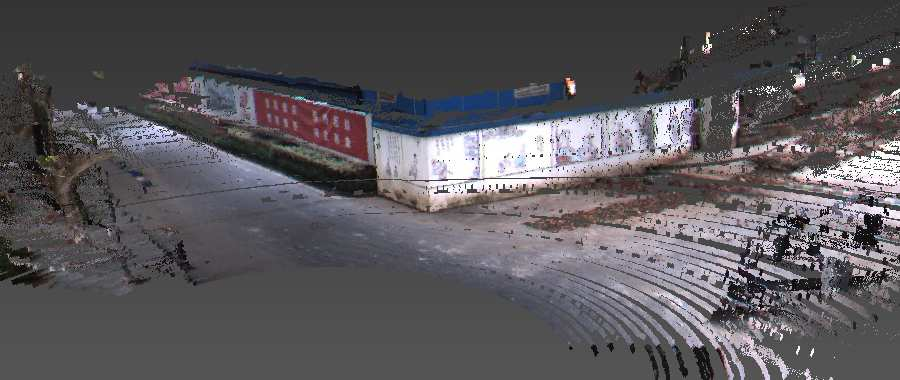
\includegraphics[width=\textwidth]{img/sensor_fusion/colored_point_cloud.png}
		\caption{Colored Point Cloud. Source~\cite{Gong2013}}
		\label{fig:colored_point_cloud_example}
	\end{subfigure}
	\quad
	\begin{subfigure}[t]{0.40\textwidth}
		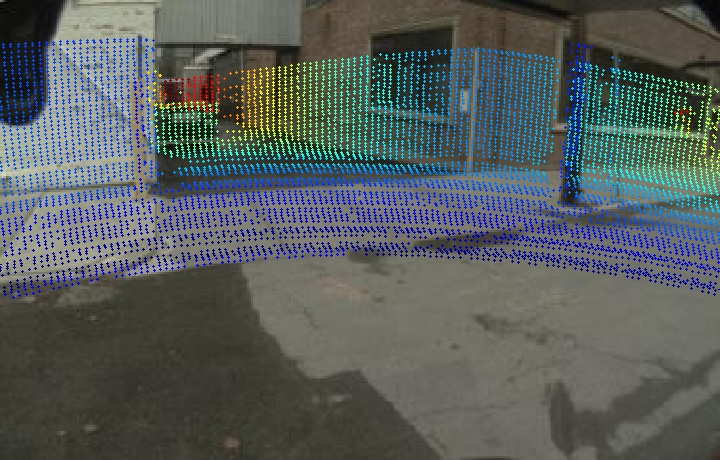
\includegraphics[width=\textwidth]{img/sensor_fusion/image_with_distance_point_cutted.png}
		\caption{Camera Image with overlapping distance measurements. Source~\cite{Bileschi2009}}
		\label{fig:image_with_lidar_distance}
	\end{subfigure}
	\caption[Examples of state of the art sensor fusion results between camera and \acs{lidar} data.]{Examples of sensor fusion between camera and \ac{lidar}. Sub-Figure~(\subref{fig:colored_point_cloud_example}) represents a colored point cloud, whose pixels are projected to the point cloud and nearby 3D points are colored with the color of their correspondent pixel. Since \ac{lidar} \ac{fov} is wider than the camera's, several points are black because no correspondences can be made. Sub-Figure~(\ref{fig:image_with_lidar_distance}) displays an image with overlapping distance measurements. Point cloud points in the image \ac{fov} are projected into the image and color mapped with intensity.}
	\label{fig:point_cloud_camera_fusion_example}
\end{figure}

There are three major types of sensor fusion: 

\begin{enumerate}
	\item \textbf{Calibration + Fusion:} Sensors are first calibrated among themselves, using one of the techniques described in Section~\ref{sec:sota:extrinsic_calibration}, and then data is converted to a referential of choice and merged;
	\item \textbf{Simultaneous Calibration and Fusion:} the implemented algorithms attempt to merge the data by minimizing an appropriated cost function. The final result consists on the multimodal merged data and the calculated extrinsic calibration parameters;
	\item \textbf{``Direct'' Sensor Fusion:} Genetic algorithms, neural networks or other similar tools analyze \ac{lidar} and camera data, without knowing any previous information about them, and output the merged data in the desired format.
\end{enumerate} 


\subsection{Calibration + Fusion}
\label{subsec:sota:calibration-and-fusion}
After calibrating the camera and \ac{lidar}, the data from these sensors can be fused, for a visual assessment of the correctness of the calibration. Some authors' whose work is referred on Section~\ref{sec:sota:extrinsic_calibration}, also show the results of sensory fusion applied to their data with the results of the proposed calibration algorithms, as a proof of calibration correctness. Unnikrishnan\etal~\cite{Unnikrishnan2005}, Velas\etal~\cite{MartinVelas2013}, Mirzaei\etal~\cite{Mirzaei2012}, Pusztai\etal~\cite{Pusztai2018} and Gong\etal~\cite{Gong2013} opt to use the camera information to color the point cloud, showing a colored point cloud (for Gong's\etal example, refer to sub-Figure~\ref{fig:colored_point_cloud_example}). Others, such as Fremont\etal~\cite{Fremont2013}, Liao\etal~\cite{Liao2019} and Park\etal~\cite{Park2014} prefer to show a visual metric of the calibration correctness by overlapping depth information gathered by the \ac{lidar} onto the image.

This sensor fusion technique is based on the application of the affine transformation described in Equation~\eqref{eq:jointRotationTranslationTransform}, which transforms data from the \ac{lidar} coordinate frame to the camera, allowing for a $3D point \leftrightarrow pixel$ mapping, enabling either point cloud coloring or overlapping the distance measurements on the image, as previously shown in Figure~\ref{fig:point_cloud_camera_fusion_example}.
	
\begin{equation}
	\label{eq:jointRotationTranslationTransform}
	\begin{bmatrix}
		X_{cam} \\
		Y_{cam} \\
		Z_{cam} \\
		1
	\end{bmatrix}
	= 
		\underbrace{
	\left[
			\begin{array}{ccc|c}
				r_{xx} & r_{yx} & r_{zx} & t_x \\
					r_{xy} & r_{yy} & r_{zy} & t_y \\
					r_{xz} & r_{yz} & r_{zz} & t_z \\
					0      & 0      & 0      & 1 
				\end{array}
		\right]
		}_\text{\large\textbf{[R|t]}}
	\begin{bmatrix}
		X_{LiDAR} \\
		Y_{LiDAR} \\
		Z_{LiDAR} \\
		1
	\end{bmatrix}
\end{equation}


\subsection{Simultaneous Calibration and Fusion}
\label{subsec:sota:simultaneous-calibration-fusion}
Li\etal proposes a method for simple indoor setups consisting of a single camera and a \ac{lidar} on a servo motor. The mechanism is rotated for three angular positions and a point cloud and image is taken for each one. Then, every image and point cloud are stitched together using fiducial features, resulting on a colored point cloud and on the determination of the calibration parameters~\cite{Li2016}. 

Park\etal also proposes a method for fusing uncalibrated \ac{lidar} and stereo camera data, using two \ac{cnn}: one for calibration, by reducing error between disparity images; and a second to refine the fused disparity maps with the left image~\cite{Park2019}. 

Yang\etal also proposes a method for stereo image and \ac{lidar} point cloud fusion using a Generalized \acl{icp} algorithm to match features and extracted a fused tridimensional refined model, at the same time it estimates the rigid body transform between camera and \ac{lidar}~\cite{Yang2017}.

Castorena\etal approach for sensor fusion matches the edges using a weighted total variation norm, fusing depth maps from a \ac{tof} camera with \ac{lidar} point clouds, useful not only for calibration, but also to refine the results of the fusion process and generate a more accurate colored point cloud~\cite{Castorena2016}.

\subsection{``Direct'' Sensor Fusion}
Still on embryonic steps, ``direct'' sensor fusion relies on deep learning to learn how to calibrate and fuse \ac{lidar} and camera data, therefore not requiring any previous knowledge about the dataset. It differs from sub-Section~\ref{subsec:sota:simultaneous-calibration-fusion} because the features and the cost function to be minimized are determined by the neural network and not projected by the researchers.

Liang\etal approach uses a multi-task multi-sensor dense fusion network for camera and \ac{lidar} fusion, that can not only fuse the data and create a colored point cloud, but also perform object detection on image and point cloud, with 3D bounding box estimation~\cite{Liang2019}.

Wei\etal research is aimed for a real-time multi-sensor collision avoidance system, on which the standalone usage of camera and \ac{lidar} does not yield satisfactory results~\cite{Wei2018}. The sensor fusion algorithm uses a \ac{cnn} and feature extraction to fuse \ac{lidar} and camera data. 

\subsection{Considerations about the different methods and our work}
On our work, since we are aiming to first calibrate the sensors and then fuse the data, following a more ``traditional'' approach to sensory data fusion, our algorithm will be based on the methods described in sub-Section~\ref{subsec:sota:calibration-and-fusion}. 

Simultaneous calibration and fusion methods (sub-Section~\ref{subsec:sota:simultaneous-calibration-fusion}) would be interesting, but the research focus to develop one of those methods would deviate our work from the \ac{lidar} interference study.

On the alternatives that rely on neural networks and deep learning, Wei\etal~\cite{Wei2018} solution is attractive, but it was only published when this work was in a final state, which made it not possible to be considered for this work.

\section{Object Detection}
\label{sec:sota:object-detection}

Object Detection is a field of \acl{cv} that intends to detect objects in an image. Currently, the most commons approach is a Deep-Learning based approach, where end-to-end object detection is possible without the need of handmade feature engineering.

%two approaches to tackle this problem are possible:

%\begin{enumerate}
%	\item \textbf{\acl{ml} based approach:} objection detection is performed on two steps: first a set of feature descriptors are chosen and extracted from reference images; secondly a \acf{nn} takes those features and perform the classification;
%	\item \textbf{Deep-Learning based approach:} end-to-end object detection without the need of handmade feature engineering.
%\end{enumerate}

%\subsection{\ac{ml} based approach}
%When referring to the first solution, Haar-like features~\cite{Messom2006}, \ac{sift}~\cite{Hughes2011a}, \ac{surf}~\cite{Bay2008} and \ac{hog} features~\cite{Dalal2010, Surasak2018} are normally used, on a Viola-Jones \ac{nn} (or its extensions)~\cite{Viola2001, ViolaP2004}. % For more details see 

\subsection{Deep-Learning based approach}
%The second solution is 
Normally implemented with a Region Proposal \acf{cnn}, developed by Girshick\etal on 2014~\cite{Girshick2014}. A common \ac{cnn} cannot be used for object detection on an image because the number of detected objects is variable, and so would be the size of the output layer, which is not possible on this architecture. A \ac{rcnn} differs from a \ac{cnn} due to the region proposal algorithm preceding it, that limits the number of regions to be evaluated on an image to approximately 2000, therefore limiting the number of objects on an image~\cite{Girshick2014}. However, this \acl{nn} needs to be run for every one of the 2 thousand regions, making it slow and infeasible for real-time object detection~\cite{Girshick2014}. One year later, Girshick proposed a new architecture called Fast \ac{rcnn}, that runs the convolutional model only once and generates a feature map and bounding box offsets, increasing the speed of its \ac{rcnn} up to 20 times and improving the \ac{map}~\cite{Girshick2015}, a common metric used to quantify the performance of \ac{nn} regarding their detection results. For further information and a formula, see~\cite{mAP, AP}.

In 2016, Shaoqing Ren\etal proposes a newer architecture that does not use a selective search for the region proposal algorithm, but instead has a Region Proposal Network to generate \ac{roi} for the proposal classification stage, called Faster \ac{rcnn}~\cite{Ren2017}. Such architecture achieves state-of-the-art object detection at a frame-rate of 5 \ac{fps}. 

Other alternatives, such as \ac{spp} Deep \ac{cnn}, exist and their details can be found in~\cite{He2015}.

While the previous \ac{nn} use separated networks for region proposal of a possible object on an image and region classification to locate a possible object on an image, \acf{yolo}, developed by Joseph Redmon, is an alternative solution that analyzes the image only once. It keeps a global context of the image while dividing it into regions and predicting bounding boxes. Those bounding boxes are weighted by the computed probabilities of each region and thresholding by the user~\cite{Redmon2016}. 

\subsection{Public Image Datasets}
To train deep learning image object detection \acp{nn}, several image datasets are available online. Two of the most relevant, considering number of labeled objects and number of images are:

\begin{itemize}
	\item \ac{pascal-voc} dataset;
	\item Microsoft \acf{coco} dataset.
\end{itemize}

\ac{coco}'s dataset has 80 object classes, containing common road objects also present on the \ac{kitti} dataset and other objects used on this research~\cite{Lin2014a}. Since \ac{pascal-voc} only has 20 object classes~\cite{Everingham2010}, being unable to detect a ball, truck and road signs, \ac{coco}'s dataset is preferred to train the image object detection \acp{cnn} weights.

\subsection{\ac{yolo}}
\ac{yolo}v2, released in 2017, can achieve, at best, 78.6 \ac{map} on the \ac{pascal-voc} 2007 dataset at 40 \ac{fps} (see more details in~\cite{Redmon2017}). \ac{yolo}v3, released in 2018, achieves, at best, 57.9 \ac{map}-50 on \ac{coco}'s dataset, at almost 20 \ac{fps} (3x faster than other networks with the same \ac{map}-50)~\cite{Redmon2018}.

\ac{yolo} runs on Darknet, an Open Source \ac{nn} framework written in C and \ac{cuda} by the same author~\cite{Redmon2013}. Darknet is configurable, supporting several network models without needed to be recompiled, such as AlexNet~\cite{Krizhevsky2007}, DenseNet~\cite{Huang2017}, ResNet~\cite{He2016}, \acp{rnn}~\cite{Cleeremans1989} and \ac{yolo}~\cite{Redmon2016}. It supports \ac{gpu} acceleration, if compiled together with Nvidia\cp~\ac{cuda}\texttrademark~library. Pre-trained weights for several image datasets and network models are available online on~\cite{Redmon2013}. 

\ac{yolo} is not the most accurate image object detection solution, but it is the only solution in the state of the art of image detection that offers a reasonable trade-off between accuracy, speed and resource usage~\cite{Redmon2018}. Therefore, it has proliferated as one of the most common \ac{nn} to be used on image detection, specially under scenarios where speed is important, such as autonomous vehicles. Therefore, \ac{yolo} is our preferred choice for an image object detection \ac{nn}.

\subsection{Cloud Based Platforms}
Several paid and cloud based alternatives exist, such as Amazon Rekognition~\cite{awsRekognition}, Google Cloud Vision \ac{api}~\cite{googlevision}, IBM Watson Visual Recognition~\cite{watson} and Microsoft Computer Vision software~\cite{azurecv}. 

Since those platforms require connectivity to the Internet, they are not good candidates to the solution we are trying to develop. Therefore, they are discarded.

\subsection{Objection Detection using \ac{lidar} and \ac{lidar} + Camera}
Out of the scope of this thesis is object detection only on \ac{lidar} data or \ac{lidar} + camera. However, as a starting point for object detection on point cloud, we recommend the work developed by Waleed Ali\etal~\cite{Ali2019}, which is an adaptation of \ac{yolo} to tridimensional data (point clouds): \ac{yolo}3D; and the work developed by Shi\etal~\cite{Shi2018}, a two part \ac{rcnn} that estimates and refines objects bounding boxes from point cloud data.

Regarding \ac{lidar} and camera simultaneous object detection, we recommend the familiarization with Complexer-\ac{yolo}, developed by Martin Simon\etal~\cite{Simon2019}, which is capable of detecting and tracking objects on point cloud and camera.


\section{\ac{lidar} Interference}
\label{sec:sota:lidar-interference}
\ac{tof} \ac{lidar}'s basic principle implies that when a \ac{laser} pulse is emitted, three different scenarios are possible, being the first one the only one that produces a valid measurement:

\begin{enumerate}
\item The \ac{laser} pulse returns, due to the reflection of an obstacle;
\item The \ac{laser} pulse does not return;
\item The \ac{laser} pulse returns with intensity below the noise floor.
\end{enumerate}

Interference and crosstalk between pairs of \acp{laser} and photodetectors on a \ac{lidar} are mitigated with different firing offsets, or in the case of mutual interference between \ac{lidar}, it is possible to synchronize their firing time using specialized clock signals~\cite{vlp16}.

However, in a society where self-driving vehicles coexist, another scenario is possible: \ac{lidar} ``A'' fires a \ac{laser} pulse that is received, directly or indirectly, by the photodetector on a \ac{lidar} ``B''. Since \ac{lidar} ``B'' measures the distance to an obstacle by measuring the time between the firing and reception of its own \ac{laser} pulse, the reception of another \ac{laser} pulse results in an erroneous measure with an unpredictable behavior. If this interference is significant, the reliability of the \ac{lidar}, and consequently autonomous vehicles and \ac{adas}, is seriously undermined due to the incapability to accurately map their surroundings.

% This problem, deeply researched for automotive \ac{radar} \cite{}, as yet to gain the attention of the research community of automotive \ac{lidar} and 


To the best of the author's knowledge, the first consideration about \ac{lidar} interference is given by Hebert and Krotkov in 1991~\cite{Hebert}. Their study was conducted for \ac{amcw} \ac{lidar} systems, and among other findings, they state that range and intensity measurements on \ac{lidar} are not completely independent, since lower intensity reflection can lead to an increase on range noise and shifts. 

In 2013, Retterath and Laumeyer~\cite{Retterath2015}, seek to provide an apparatus for an array based system with reduced interference. Their patented work is an array \ac{lidar} that has lower probability of crosstalk than other solutions, which was latter patented worldwide~\cite{Retterath2015WO}. In 2016, another patent is filled for the same array based \ac{lidar}~\cite{Retterath2016}, this time for object detection and in 2017, Facet Technology, the patent applicant, sends out a Press Release indicating that they have developed a \textit{``Safe and Secure\acs{lidar}\cp~Crosstalk Elimination Licensing Program''}, and that they have experienced crosstalk interferences up to 2\%~\cite{Facet}.

In 2017, Velodyne Inc., the world leader and  major manufacturer of mechanical rotating \ac{lidar}, filled a patent on a new implementation that reduces crosstalk~\cite{Hall2017}. Their focus is to solve inter-channel crosstalk, but multi-\ac{lidar} crosstalk reduction is also referred on the patent.

In 2018, Axel Diehm\etal proposes a spatial temporal filter for eliminating a crosstalk problem between two Velodyne HDL-64 \acp{lidar}~\cite{Hebel2018}. Their crosstalk behaviour is well-defined as an area of interfered points at a particular orientation, and their work is focused on how to filter out those points. They also partially expanded their analysis to the time domain of interference. Nonetheless, a root cause for the crosstalk behavior was not provided.

\subsection{Autonomous vehicles hacking through \ac{lidar} Interference}
Jonathan Petit\etal presents a study on how to remotely attack automotive cameras and \acp{lidar} on vehicles~\cite{Petit2015}. They explore several methods of attack, such as relay, replaying and spoofing. Petit's work shows, for laboratory scenarios, how to make obstacles disappear and how to make the \ac{lidar} see ``ghost'' objects, for distances further than the distance of the spoofer. 

Hocheol Shin\etal, two years later, presented an improved method that not only is able to spoof obstacles at a distance further than the distance of the spoofer, but also closer~\cite{Shin2017}. His work used common \acp{lidar}, such as Velodyne VLP-16~\cite{vlp16}. Shin\etal also found that the curved reception glass of \acp{lidar} allow for reflection of an attacking light source inside its case, allowing the attacker to be at a different direction that of the perceived attack. Despite their work being extremely experimental and not directly applied on real world scenarios, due to the laser alignment required for an effective attack on real driving scenarios, Petit\etal and Shin\etal research show that it is possible to attack a \ac{lidar} sensor and interfere with its measurements. Some results from Shin's research are shown in Figure~\ref{fig:shinInterference}.

\begin{figure}[!ht]
	\centering
	\begin{subfigure}[c]{0.4\textwidth}
	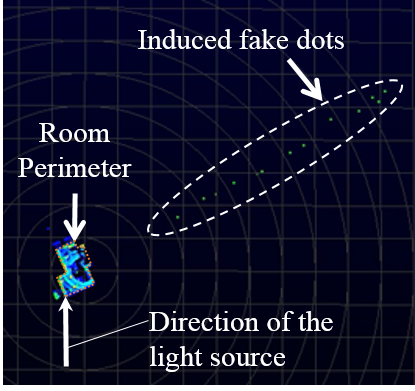
\includegraphics[width=\textwidth]{img/lidar/interference_angle_control.png}
\caption{}%Spoofing an obstacle at a different angle of the spoofer}
		\label{fig:shinInterferenceAngle}
	\end{subfigure}
	\quad
	\begin{subfigure}[c]{0.55\textwidth}
		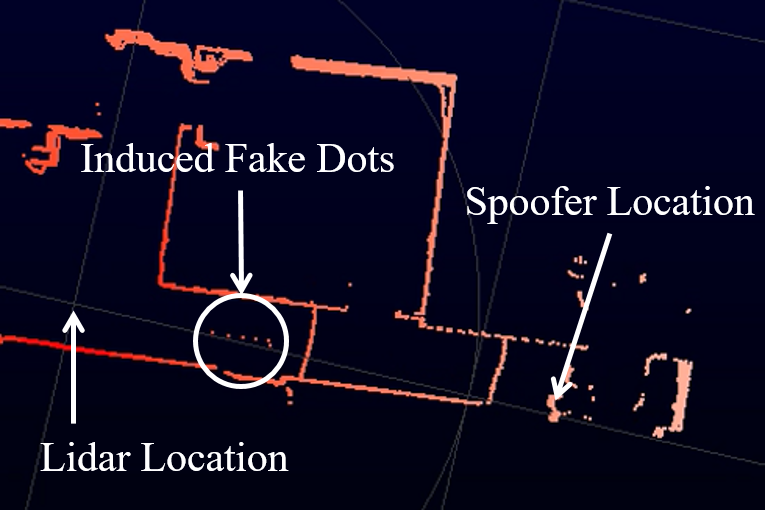
\includegraphics[width=\textwidth]{img/lidar/interference_distance_control.png}
	\caption{}%Spoofing an obstacle at a closer distance than the spoofer}
		\label{fig:shinInterferenceDistance}
	\end{subfigure}
	\caption[Spoofing obstacles on \ac{lidar} at different angles and closer distances that the spoofer.]{Spoofing examples on a Velodyne VLP-16 \ac{lidar}, extracted from Source~\cite{Shin2017}. Sub-Figure~(\subref{fig:shinInterferenceAngle}) shows the spoofed object at a different angle of the spoofer and sub-Figure~(\subref{fig:shinInterferenceDistance}) shows the spoofed object at a different distance than the spoofer.}
	\label{fig:shinInterference}
\end{figure}


\subsection{Two-Dimensional Coplanar \ac{lidar} Interference}
Gunzung Kim\etal, in 2015, presents the first results on multiple \ac{lidar} interference on their three papers~\cite{Kim2015a, Kim2015b, Kim2015c}. The three papers are based on a SICK LMS-511, a 2D \ac{lidar}\footnote{A single \ac{laser} and photodetector are mounted on a rotating device, measuring several azimuthal angles when the motor rotates, but the polar angle is kept fixed, scanning a single line of the environment.}. Kim\etal setups consist of a box with $\SI{5.3}{\meter} \times \SI{4}{\meter}$~\cite{Kim2015a} or $\SI{5.3}{\meter} \times \SI{5.3}{\meter}$~\cite{Kim2015b, Kim2015c}, with the \acp{lidar} positioned inside. The walls are made of a non-glossy wood and the experimental setup is shown in Figure~\ref{fig:kim-setups}. His classification of interference is based on the determination of a majorant and minorant for the distance of the wall, with a 10\% tolerance around the mean value.

\begin{figure}[!ht]
	\centering
	\begin{subfigure}[c]{0.45\textwidth}
		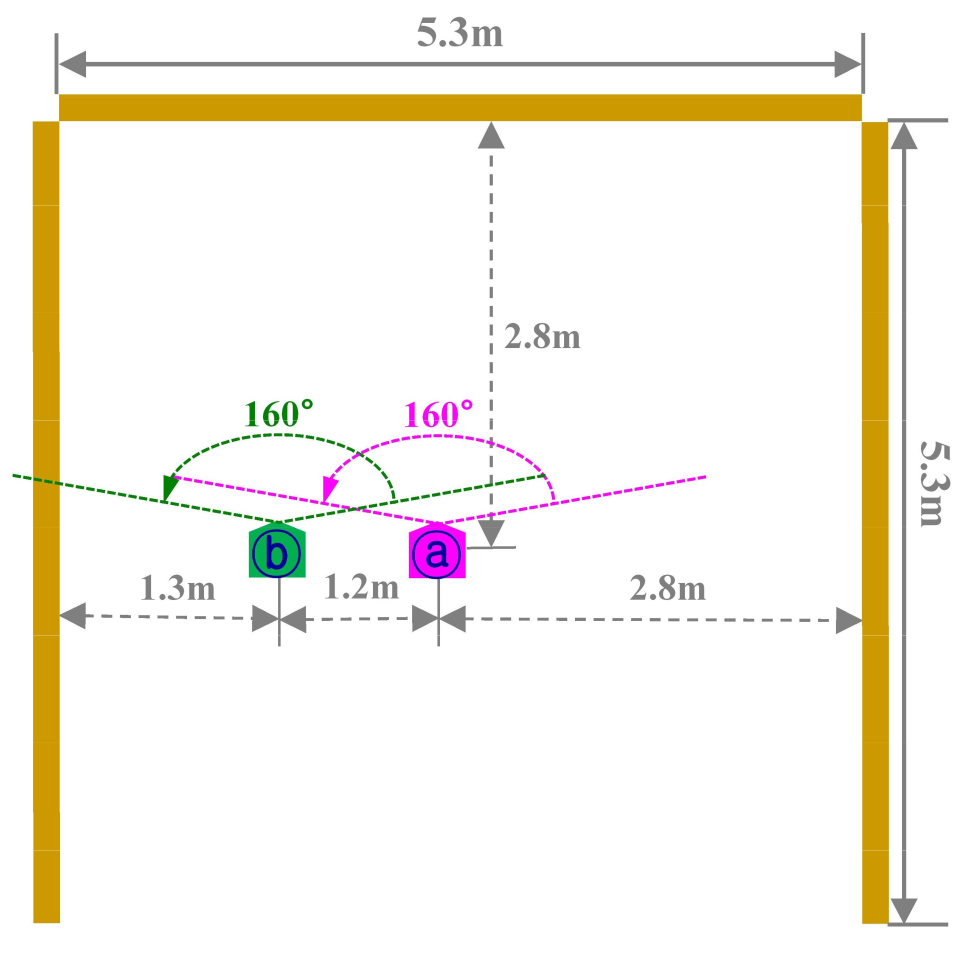
\includegraphics[width=\textwidth]{img/lidar-interference/kim-setup-side-by-side-1.png}
		\caption{\textit{Side-by-Side \#1}.}
		\label{fig:kim-side-by-side-1}
	\end{subfigure}
	\quad
	\begin{subfigure}[c]{0.45\textwidth}
		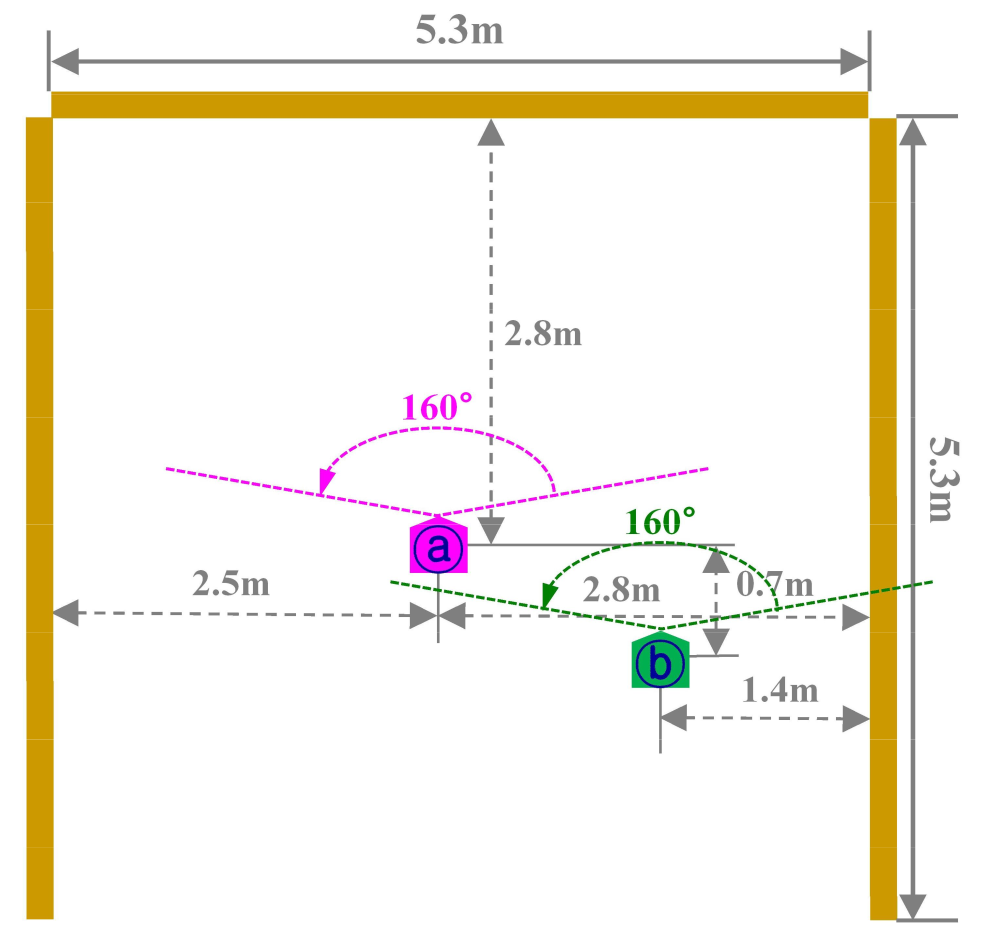
\includegraphics[width=\textwidth]{img/lidar-interference/kim-setup-side-by-side-2.png}
		\caption{\textit{Side-by-Side \#2}.}
		\label{fig:kim-side-by-side-2}
	\end{subfigure}
	\\ \vspace{4mm}
	\centering
	\begin{subfigure}[c]{0.45\textwidth}
		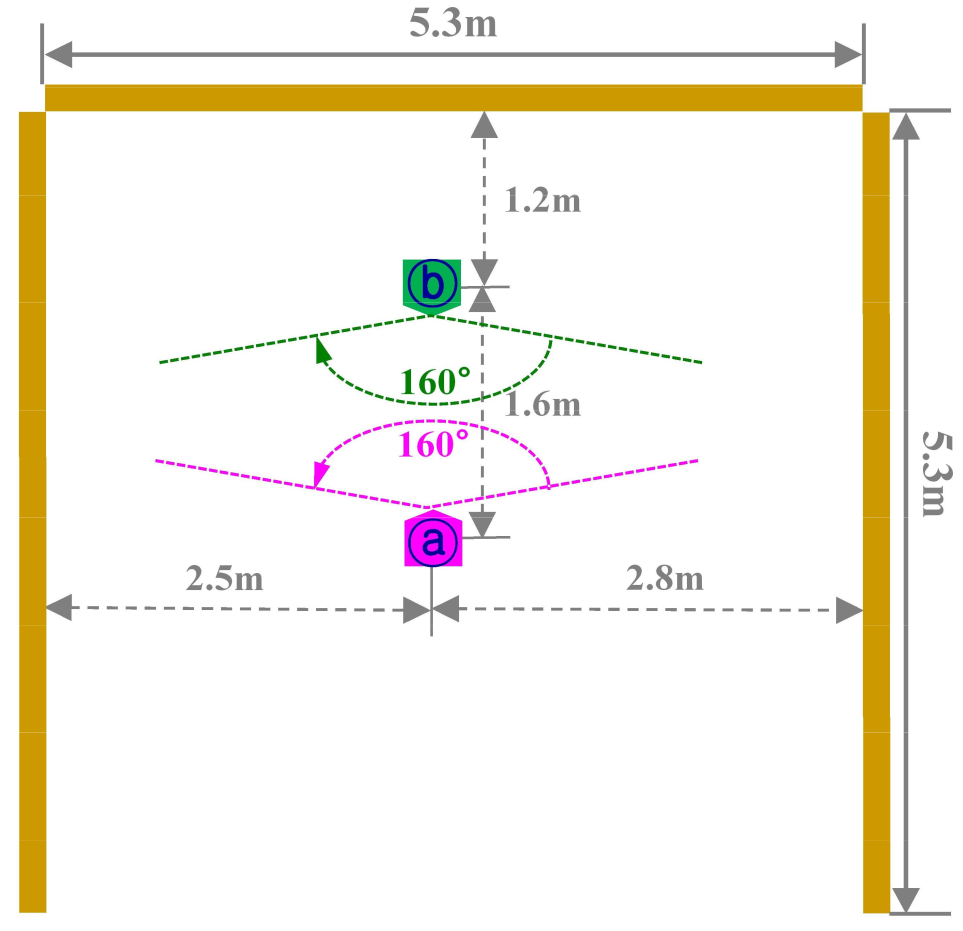
\includegraphics[width=\textwidth]{img/lidar-interference/kim-setup-face-to-face.png}
		\caption{\textit{Face-to-Face}.}
		\label{fig:kim-face-to-face}
	\end{subfigure}
	\quad
	\begin{subfigure}[c]{0.45\textwidth}
		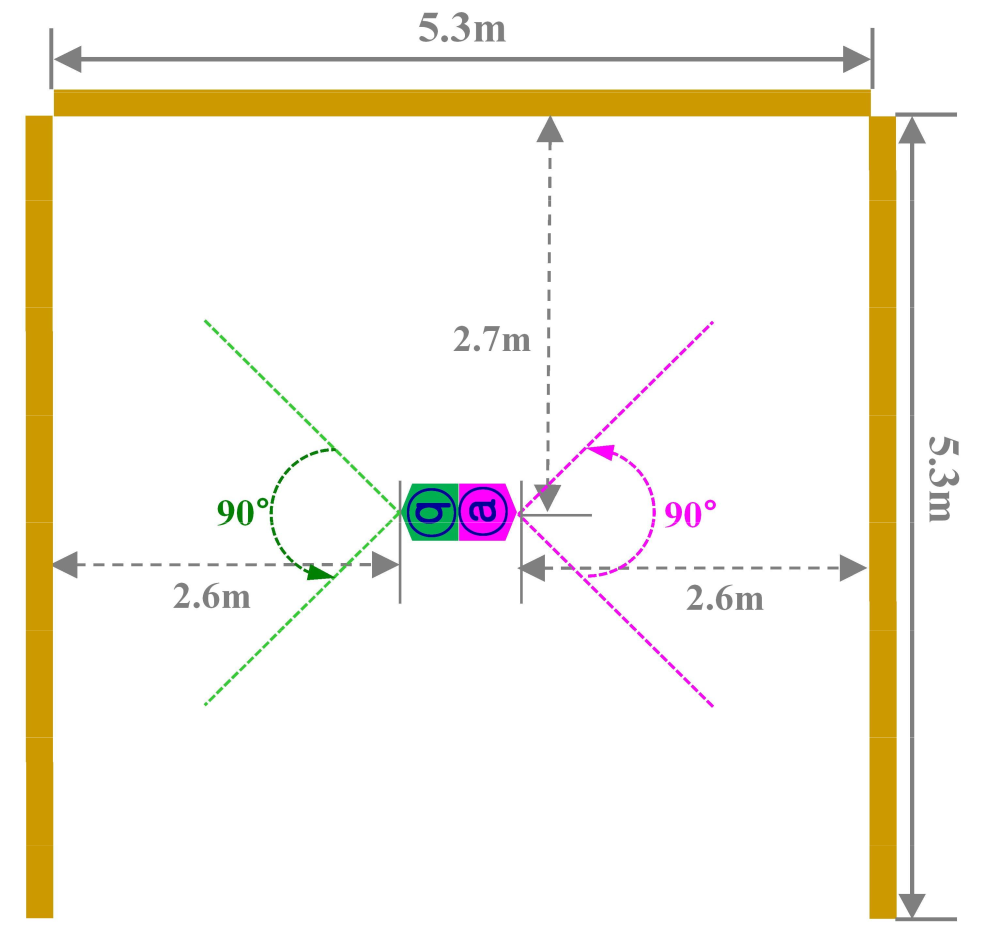
\includegraphics[width=\textwidth]{img/lidar-interference/kim-setup-back-to-back.png}
		\caption{\textit{Back-to-back}.}
		\label{fig:kim-back-to-back}
	\end{subfigure}

	\caption[Experimental setups used by Kim\etal and Popko\etal for 2D \ac{lidar} interference studies.]{Experimental setups devised by Gunzung Kim\etal, as detailed on~\cite{Kim2017}. Sub-Figure~(\subref{fig:kim-side-by-side-1}) and (\subref{fig:kim-side-by-side-2}) consist of an interference setup where the victim and interferer \ac{lidar} are adjacent to each other. Sub-Figure~(\subref{fig:kim-face-to-face}) tests the interference when the two \acp{lidar} are on each other \ac{fov} and sub-Figure~(\subref{fig:kim-back-to-back}) when the \acp{lidar} are not on each other \ac{fov}.}
	\label{fig:kim-setups}
\end{figure}


% Kim \etal research despite using a 2D \ac{lidar} instead of a 3D \ac{lidar} is the only study to use two independent 2D \ac{lidar}s interfering with each other. Kim \etal results indicate that interference has spatial and temporal locality \cite{Kim2015} and in any given time, in Kim's setup, a data point has 0.05 \% probability of being interfered \cite{Kim2015}. The former states that if a particular angle is interfered, the following angles are likely to also be interfered; while the latter indicates that if a measure is interfered, on the following frame that same measure is also likely to be interfered. 

Kim\etal tests show the temporal and spatial locality of the data. Temporal locality implies that a given angular direction is more likely to be interfered if it was interfered in the past, indicating that interference persists through time. Spatial locality implies that, for a current scan, if an interference occurs, it is more likely that the next angle will also be interfered, indicating that interference persists through space. 

The experiment conducted in~\cite{Kim2015a} captured a ground-truth model for 4 hours and the interference data for 50 hours. For a given angle position, Kim concluded that for his experimental setup, 4.4\% of the total number of full line scans were interfered, but that number only translates to one in every 2000 point (0.05\% interfered points for the total number of registered points). When considering the nature of interference, spatial interference is rare: 78\% of the interfered points are not interfered on their next measurement (against 15\% that are), and only 7\% of the angular positions are interfered consecutively 3 or more times, for a record of 13 (meaning \SI{0.5}{\second} of interference). For consecutive interference on nearby azimuthal angles on the same scan, only 30\% of the interference happens within single angular step and 26\% on a second. The largest consecutive number of angles with interference are 102, which translates to \SI{25.5}{\degree}.

In~\cite{Kim2015b}, Kim~\etal reports new tests on \ac{lidar} interference, adding two new tests: a side-by-side with a small displacement and a face-to-face test. In~\cite{Kim2015c} a back-to-back test is also performed. Note that despite the experimental setup \textit{Side by side \#1} (Figure~\ref{fig:kim-side-by-side-1}) being identical to the setup on~\cite{Kim2015a}, disagreements on all evaluated metrics occur. Therefore, for this test, the results discussed before, taken from~\cite{Kim2015a}, and results presented in Table~\ref{tab:kim_2015_results}, based on~\cite{Kim2015b, Kim2015c}, are not in agreement. No explanations are provided for such difference and the issue is not addressed by Kim\etal on~\cite{Kim2015b, Kim2015c}.

\begin{table}[!ht]
	\centering
	\renewcommand{\arraystretch}{1.3}
	\begin{tabular}{@{}p{3.5cm}C{3cm}C{4cm}@{}}
			\toprule
			Experimental Setup Codename & \% of Lines Interfered & Relative Frequence of Interfered Points \\
			\midrule
			Side-by-side \#1 & $1.795$                & $3.103\E^{-5}$  \\
			Side-by-side \#2 & $10.33$                & $1.667\E^{-4}$ \\ \midrule
			Face-to-Face     & $1.433$                & $2.583\E^{-5}$  \\ \midrule
			Back-to-Back A   & $0.211$                & $3.387\E^{-6}$  \\
			Back-to-Back B   & $0.216$                & $3.514\E^{-6}$  \\ \bottomrule
		\end{tabular}
		\caption[Summary of Kim's\etal \ac{lidar} interference results.]{Summary of Kim's\etal the interference results from~\cite{Kim2015b, Kim2015c}, for all tests. In the second column, the percentage of lines with a single interfered point are presented. The third column corresponds to the relative frequency of interfered point for all the points.}
	\label{tab:kim_2015_results}
\end{table}

The results of the second column, \textit{\% of Lines Interfered}, characterizes the number of lines on which interference as been found. For every test scenario on this column, the line interference caused are mostly non-consecutive (above 90\% for Face to Face and 94.3\% for all the other tests).

The third column, \textit{Relative Frequence of Interfered Points}, characterizes the number of points that have been interfered regarding all points taken. The relative frequency of the interference is low, with the relation between the interfered and the total number of points being on the order of magnitude of $10^{-6}$ to $10^{-4}$. Despite the maximum of consecutive spatial interference (4 scans), more than $99.7\%$ of all interferences happen isolated on a given azimuth angle, with no repetition on the next scan for the same interfered angle~\cite{Kim2015c}. 



% To the best of the author's knowledge, despite the relevance of the topic to a society of self-driving cars, there are only three different studies available


In 2017, Kim\etal present the results on the above papers~\cite{Kim2015a, Kim2015b, Kim2015c}, extending its research by performing an intensity analysis~\cite{Kim2017}. His findings are that on a mutual interference scenario, the intensity of the received \ac{laser} pulses varies significantly, confirming Hebert and Krotkov early findings that on a \ac{lidar} system range and intensity measures are not completely independent and interfering with one affects the results of other~\cite{Hebert}.

In the same paper, he also introduces a theoretical analysis of the multipath interference based on a Lambertian distribution for modelling the reflections on the walls~\cite{Kim2017}. The model lacks generality, as it assumes average values for several parameters and some simplifications on the multipath interference, but allows to conclude that:

\begin{enumerate}
	\item After the second reflection on an obstacle, the attenuation suffered by the light beam is not sufficient for the receiving \ac{lidar} to detect it as an interference;
	\item Direct interference (on Kim's experimental setup and hardware) is likely to saturate the receiver of the interfered \ac{lidar}, which may or may not be considered a valid measurement by the hardware;
	\item Indirect interference with only one reflection can be interpreted as a valid measurement, since the intensity of the received interfered beam is similar to the intensity of a valid measurement beam.
\end{enumerate}

In 2019, Gerald Popko\etal~\cite{Popko2019a} presents a mathematical description on how stationary, coplanar and circular 2D scanning \ac{lidar} can interfere through beam path interference of the optical \ac{fov}. Based on his description, he repeats Kim's\etal experiments (see Figure~\ref{fig:kim-setups}), proposing a new statistical interference detector, instead of Kim's maximum distance minorant and majorant~\cite{Kim2015a}, and also performs a Monte-Carlo simulation~\cite{Popko2019b}. Popko\etal findings are that:

\begin{enumerate}
	\item The interference behavior depends majorly on the target geometry and beam intersection, and not on radiometric considerations;
	\item Simulating the \ac{lidar} interference is not yet reliable, since for the model developed only the scattered interference provided a value close to the real value measured;
	\item The direct interference is dominant over the scattering interference;
	\item The direct interference is mainly responsible for small distance measurement errors, while scattering interference is mainly present for large distance measurement errors.
\end{enumerate}

Lastly, Popko \etal interference results are two orders of magnitude higher than Kim's \etal measurements, $1.041 \%$~\cite{Popko2019b} vs $0.05\%$~\cite{Kim2015a}.

\subsection{A departing note on \ac{lidar} interference}
On a departing note, \ac{tof} \ac{lidar} is the mainstream \ac{lidar} for autonomous vehicles and the automotive industry, while being the less robust to crosstalk from other \ac{tof} \acp{lidar}. So far, the studies presented on \ac{lidar} interference are scarce and not representative, focused only on two-dimensional \acp{lidar}, i.e., \acp{lidar} that only scan a single line. Answers about the relevance of \ac{lidar} interference are yet to be given and more tests are required, to fully profile the interference and its impacts on autonomous driving. Robust alternatives to crosstalk, both from a technological and signal processing standpoint are also desirable.

\chapter{Camera and \acs{lidar} Calibration}
\label{chapter:calibration}

The focus of this chapter is to detail the considerations and procedures used on sensory calibration, starting by describing the experimental setup. Then, the method used to calibrate the camera and \ac{lidar} intrinsic parameters are detailed and results are shown. After properly intrinsic calibration, the two sensors can be calibrated amongst themselves, through an extrinsic calibration procedure. This procedure is explained from a mathematical standpoint and the implementation is here detailed, along with results.


\section{Experimental Setup}
\label{sec:calibration:experimental-setup}
The experimental setup is shown on Figure~\ref{fig:experimental-setup}. It consists of an industrial camera with an objective lens, a \ac{tof} \ac{lidar}, an Ethernet switch and a power source (not shown on the figure). The setup is constructed using Thorlabs\cp~Optomechanic material to mount the camera and \ac{lidar}.

\begin{figure}[!ht]
	\centering
	\begin{subfigure}[c]{0.45\textwidth}
		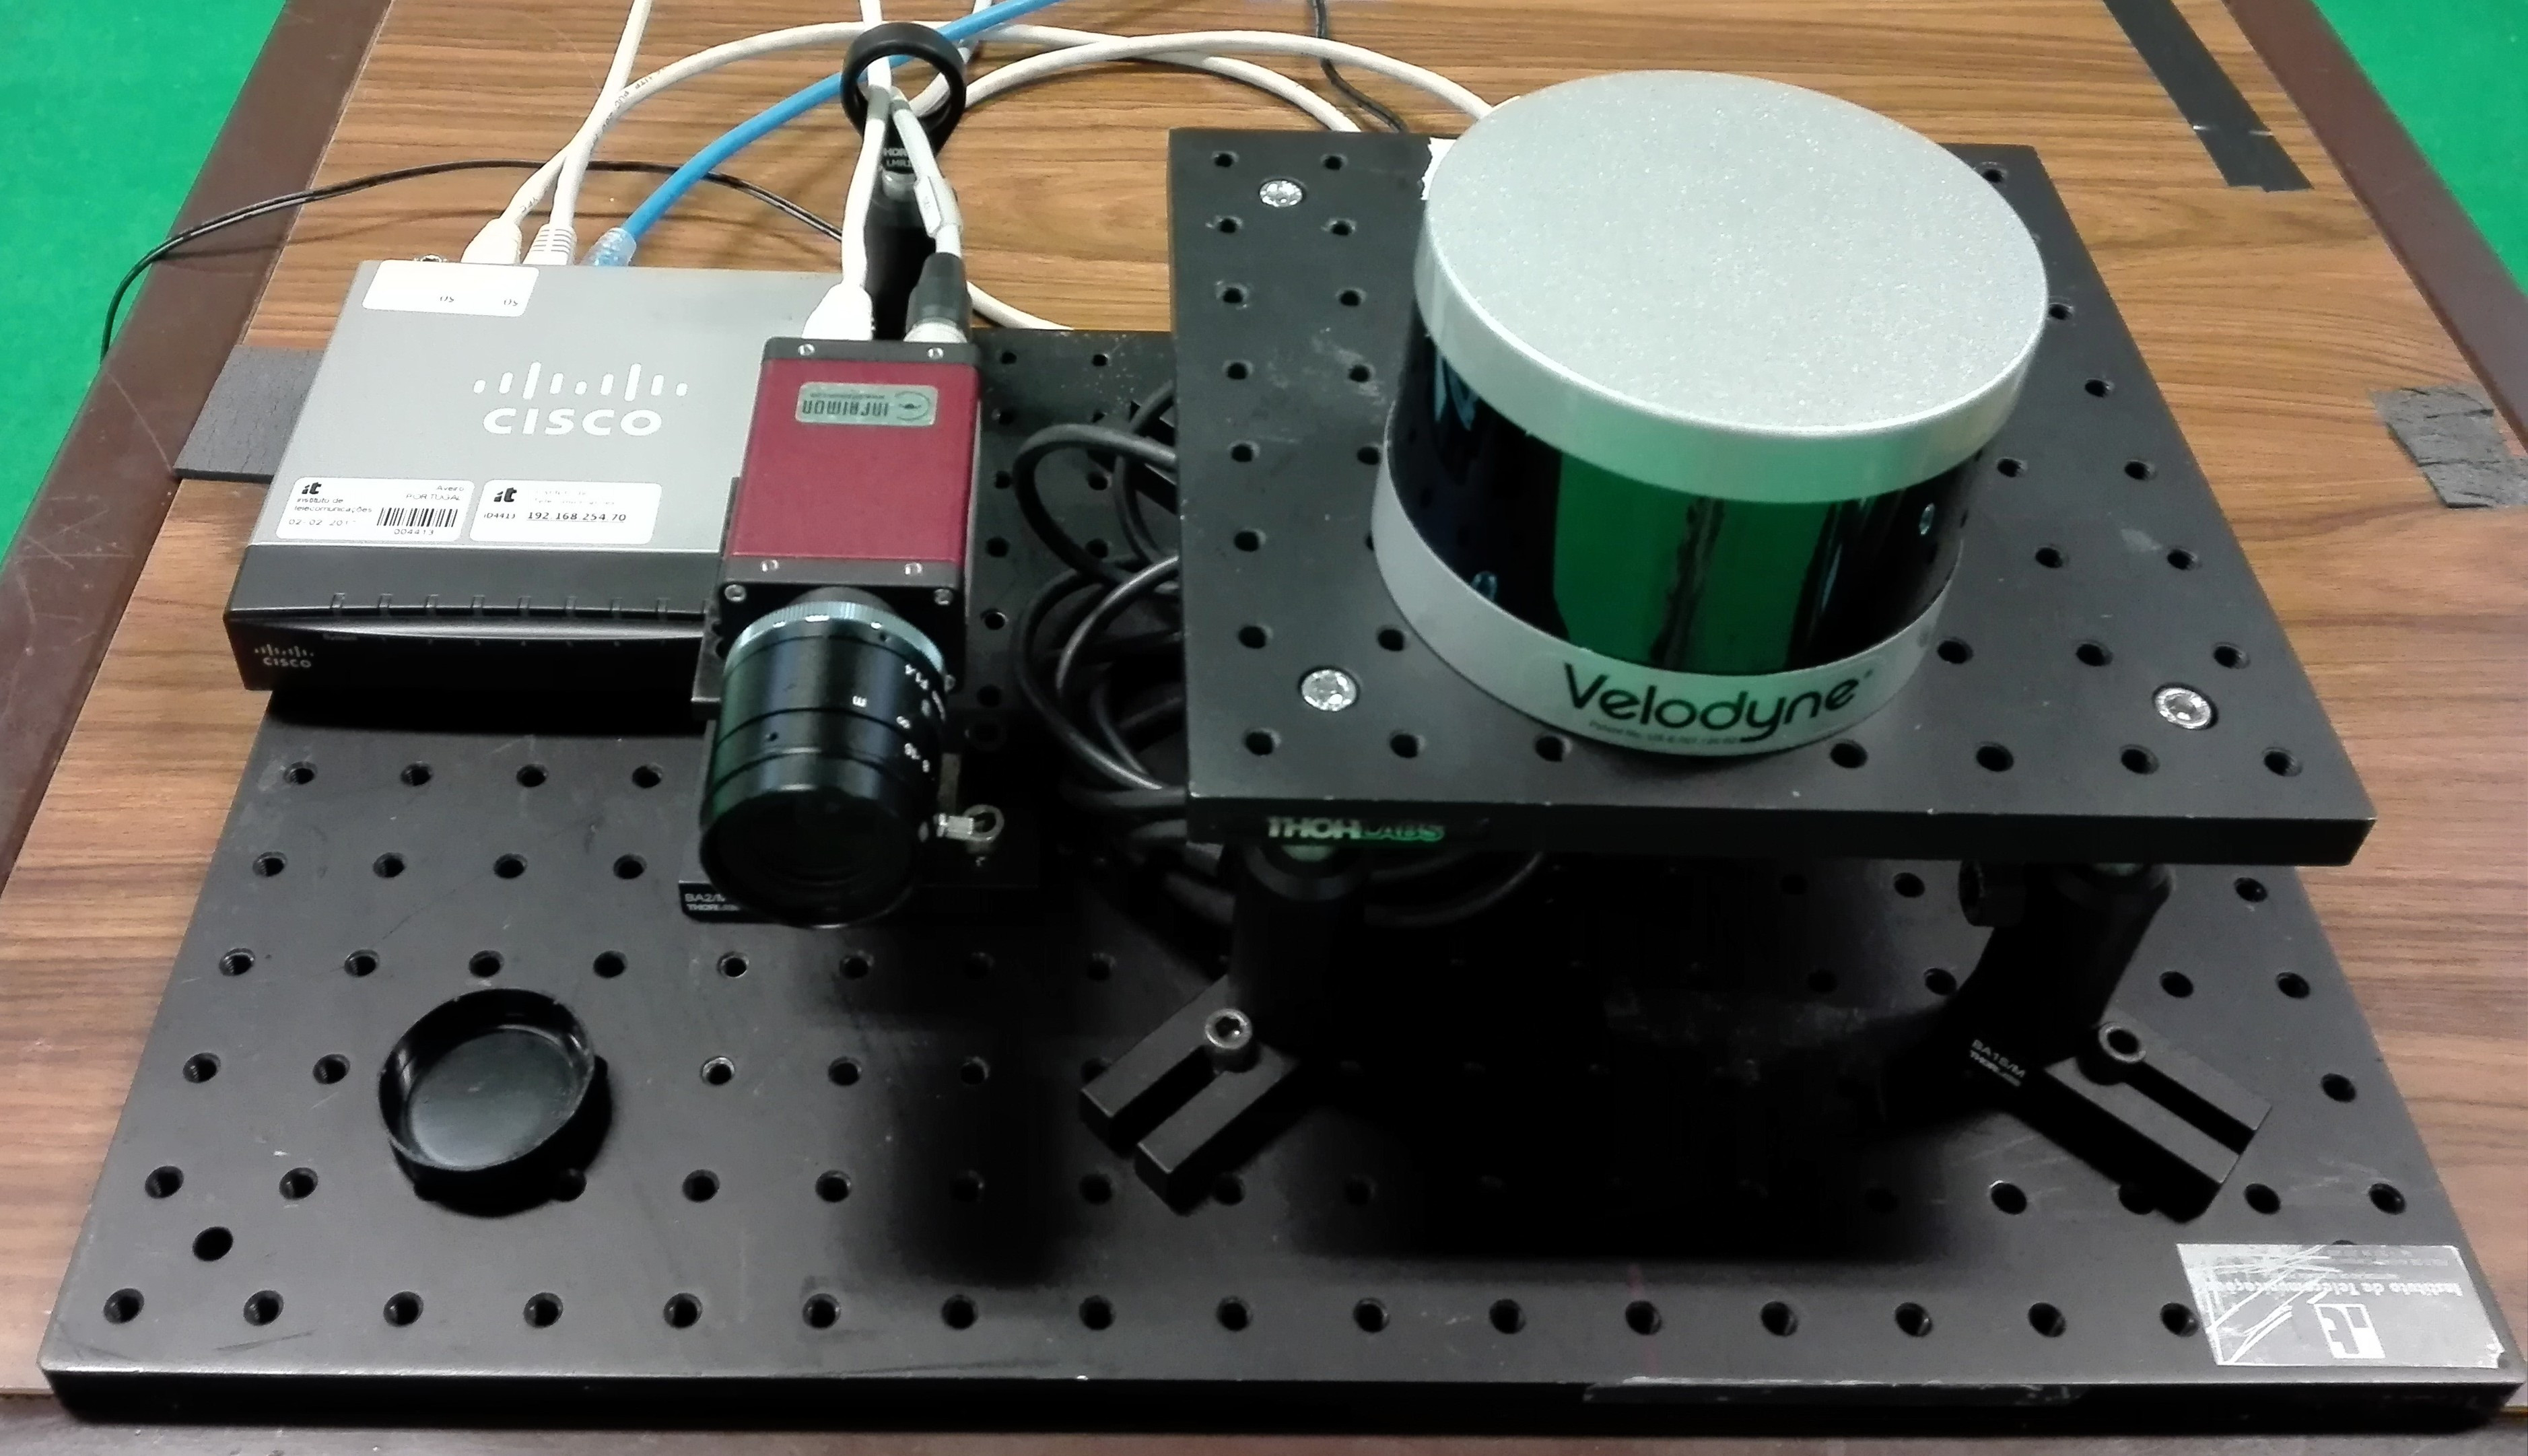
\includegraphics[width=\textwidth]{img/experimental-setup/table-setup-cambada-perspective.jpg}
		\caption{}
		\label{fig:experimental-setup:perspective}
	\end{subfigure}
	\qquad
	\begin{subfigure}[c]{0.45\textwidth}
		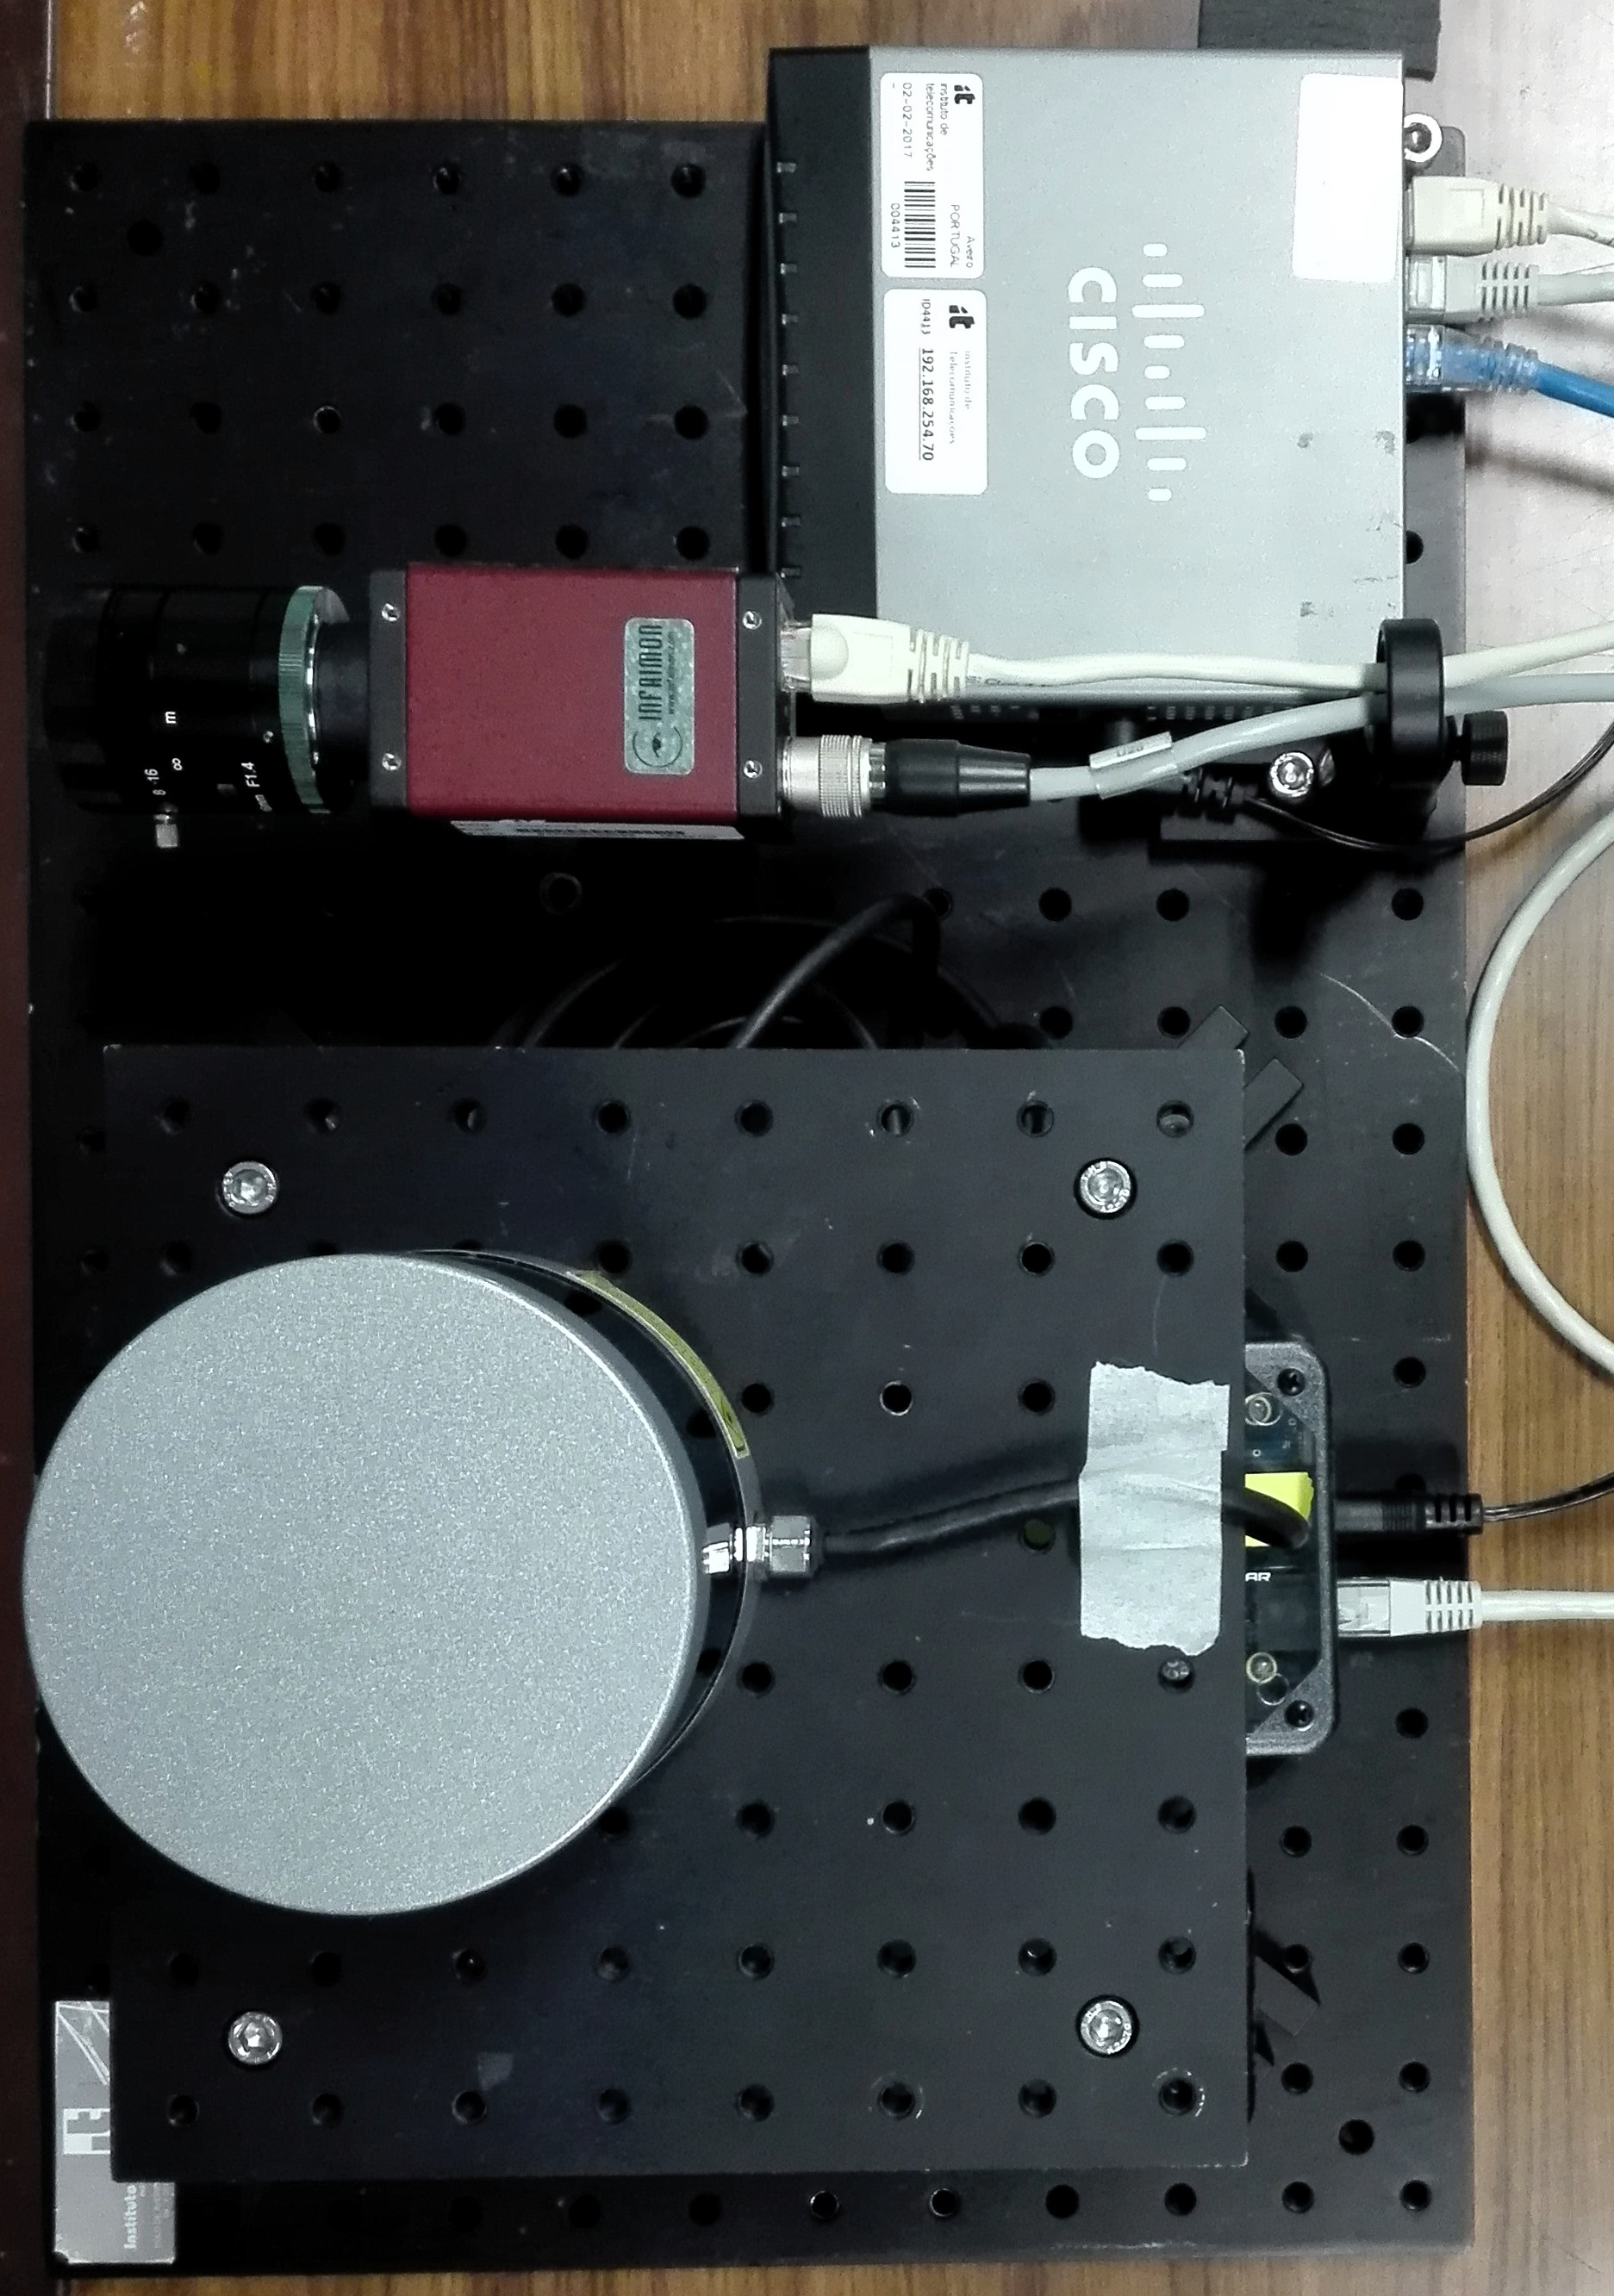
\includegraphics[width=0.65\textwidth, keepaspectratio, angle=90]{img/experimental-setup/table-setup-cambada-birds-eye.jpg}
		\caption{}
		\label{fig:experimental-setup:birds-eye}
	\end{subfigure}
	\caption[Perspective and top views of the experimental setup for the camera and \acs{lidar}.]{Relative positioning of the devices on the experimental. The \ac{lidar} is on an elevated platform to guarantee that the camera and Ethernet switch are not on its \ac{fov}. Sub-figures show the experimental setup viewed (\subref{fig:experimental-setup:perspective}) in perspective; (\subref{fig:experimental-setup:birds-eye}) from the top.}
	\label{fig:experimental-setup}
\end{figure}

\subsection{Camera and Lens}
The camera used is an industrial 5 \ac{mp} RGB camera, from \acf{avt}, model Manta G-504C. The objective is a C-Mount lens with lock from Thorlabs\cp, model MVL16M1. The full camera specifications can be accessed on~\cite{MantaG504C} and the full lens specifications on~\cite{Thorlabs}. Relevant specifications of the camera and lens are summarized  on Table~\ref{tab:camera-and-lens-specs}. 

\begin{table}[!ht]
	\renewcommand{\arraystretch}{1.2}
	\centering
	\begin{tabular}{@{}lp{7cm}l@{}}
		\toprule
		\multicolumn{2}{l}{Specification} & Value \\ \midrule
		\multicolumn{2}{l}{\emph{Camera}} & \\
		\phantom{a} & Full Resolution (width vs height) & $2452 \times 2056$ pixels \\
									& Shutter mode & Global \\
									&	Maximum \ac{fps} at full resolution & $9.2$ \\ 
									& \acs{adc}\footnotemark bit depth & $12$ bit \\\midrule 
									\multicolumn{2}{l}{\emph{Lens}} \\
									&	Focal Length & $16$ mm \\
									&	Max aperture & $f/1.4$ \\
									&	Minimum Object Distance & $300$ mm  \\
		\bottomrule
	\end{tabular}
	\caption[Relevant specifications of the camera and its lens.]{Relevant specifications for \ac{avt} Manta G-504C RGB camera (from~\cite{MantaG504C})  and MVL16M1 Thorlabs\cp~lens (from~\cite{Thorlabs}).}
	\label{tab:camera-and-lens-specs}
\end{table}

\footnotetext{\acs{adc} stands for \acl{adc}}

To power the Manta G-504C, a benchtop power source was used. Further details about powering the camera and its electrical connections are presented on Appendix-B~\ref{sec:appendix-b}.

\subsection{\ac{tof} \ac{lidar}}
The \ac{tof} \ac{lidar} used is a Velodyne VLP-16\texttrademark, a 16 beam \ac{lidar} that operates with a wavelength of \SI{903}{\nano\meter}. VLP-16 supports various measurements modes based on the return pulse (Strongest, Last, Dual) and can be connected to a \ac{gps} receiver for geopositioning and synchronization with an external clock. It also supports several rotation speeds, from 300 to 1200 \ac{rpm}, which result in different angular steps and point cloud refresh rate. The full specifications can be accessed on~\cite{VLP16} and the relevant specifications for this work are summarized on Table~\ref{tab:vlp16-specs}.

\begin{table}[!ht]
	\renewcommand{\arraystretch}{1.2}
	\centering
	\begin{tabular}{@{}p{8.3cm}l@{}}
		\toprule
		Specification & Value \\ \midrule
		Wavelength    & \SI{903}{\nano\meter} \\
		Motor \acs{rpm} & $600 \pm 3$ \\
		Angular step & \SI{0.2}{\degree} \\
		Vertical \ac{fov} & \SI{30}{\degree} \\
		Horizontal \ac{fov} & \SI{360}{\degree} \\
		Maximum Scanning Distance & \SI{100}{\meter} \\
		Theoretical Typical Distance Error & \SI{2}{\centi\meter} \\
		\bottomrule
	\end{tabular}
	\caption[Velodyne\cp~VLP-16 relevant\texttrademark relevant specifications.]{Velodyne VLP-16 relevant specifications. Source~\cite{VLP16}.}
	\label{tab:vlp16-specs}
\end{table}


\subsection{Connection Setup} 
Both Velodyne VLP-16 and \ac{avt} Manta G-504C operate over Gigabit Ethernet. Therefore, a Gigabit  Ethernet switch is required to connect all the equipment to a single computer using a single Ethernet port. The switch used was Cisco SG200-08, an 8-Port Gigabit Smart Switch. 

The switch was configured so that every port was on the same \ac{vlan}, ensuring packets were accessible on the computer, since the sensors were configured to broadcast the packets. An alternative to this implementation was to redirect the packets from each sensor to the computer network and filter the packets from the computer to the sensors, by putting them on separated networks and create a network traffic management solution. Using \ac{ros} capabilities to measure packet delay and rate of publishing of the data messages, no bandwidth constraints or packet delay/loss were verified. Therefore, the solution chosen was the former, due to its simplicity. 

For each device a fixed \acf{ip} address was attributed, following the instructions on their datasheet~\cite{VLP16, MantaVision2013}. The \ac{ip} addresses can be consulted on Table~\ref{tab:experimental-setup-ip}.

\begin{table}[!ht]
	\renewcommand{\arraystretch}{1.2}
	\centering
	\begin{tabular}{@{}lcc@{}}
		\toprule
		Device          & \ac{ip} Address & Subnet Mask\\ \midrule
		Computer        & 192.168.10.77  & 255.255.255.0 \\
		Manta G-504C    & 192.168.10.1   & 255.255.255.0 \\
		Velodyne VLP-16 & 192.168.10.201 & 255.255.255.0 \\
		\bottomrule
	\end{tabular}
	\caption[\acs{ip} addresses and subnet masks for the devices connected on the experimental setup.]{\ac{ip} addresses and subnet masks for the devices connected on the experimental setup.}
	\label{tab:experimental-setup-ip}
\end{table}

\subsection{\ac{lidar} and Camera Interference}
No significant interference is expected between the camera and the \ac{lidar}. Despite the camera lens having a transmission coefficient of $66\%$ at $\approx 900 nm$~\cite{Thorlabs}, and Sony ICX655, the camera sensor for the \ac{avt} Manta G-504C, having a Quantum Efficiency of $\approx 5\%$~\cite{MantaG504C}, \ac{avt} Manta G-504C is equipped with an \ac{ir} cut-filter.

Despite the low sensibility of the camera and the presence of an \ac{ir} cut-filter, an experiment was conducted to verify the occurrence of interference. The experimental setup was switched on in a Dark Room without any other light sources and the camera feed was visualized. Besides the noise caused by the camera electronics operation, no signs of interference caused by the \ac{lidar} infrared beams could be observed on the camera image feed, since no bright spots were found. Therefore, no further work on \ac{lidar} to camera interference were carried


%\begin{figure}[H]
%	\centering
%	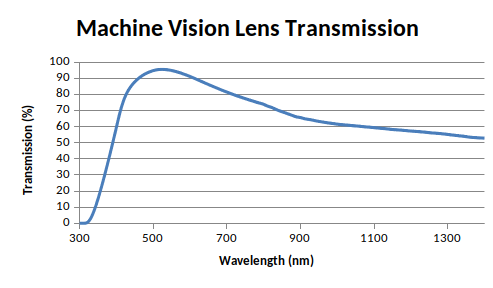
\includegraphics[width=0.6\textwidth]{img/experimental-setup/lens-transmission.png}
%	\caption{Transmission of the MVL16M1 lens in relation the light wavelength. Source~\cite{Thorlabs}}
%	\label{fig:lens-transmission}
%\end{figure}



\section{Camera Intrinsic Calibration}
\label{sec:calibration:camera}
The act of calibrating a camera consists on determining its intrinsic parameters, as detailed in sub-Section~\ref{subsec:sota:camera-intrinisc-calibration}. This can be done by taking different images with a known pattern, fully visible on the camera \ac{fov}, changing its rotation and translation in relation to the camera coordinate frame.

The calibration procedure undertaken uses a chessboard of $13 \times 9$ squares, with each square having an edge length of \SI{44.0}{\milli\meter}. The chessboard used can be seen on Figure~\ref{fig:chessboard}. It was laser printed on a \SI{100}{\gram} A2 paper and then glued to a plywood board.

\begin{figure}[H]
	\centering
	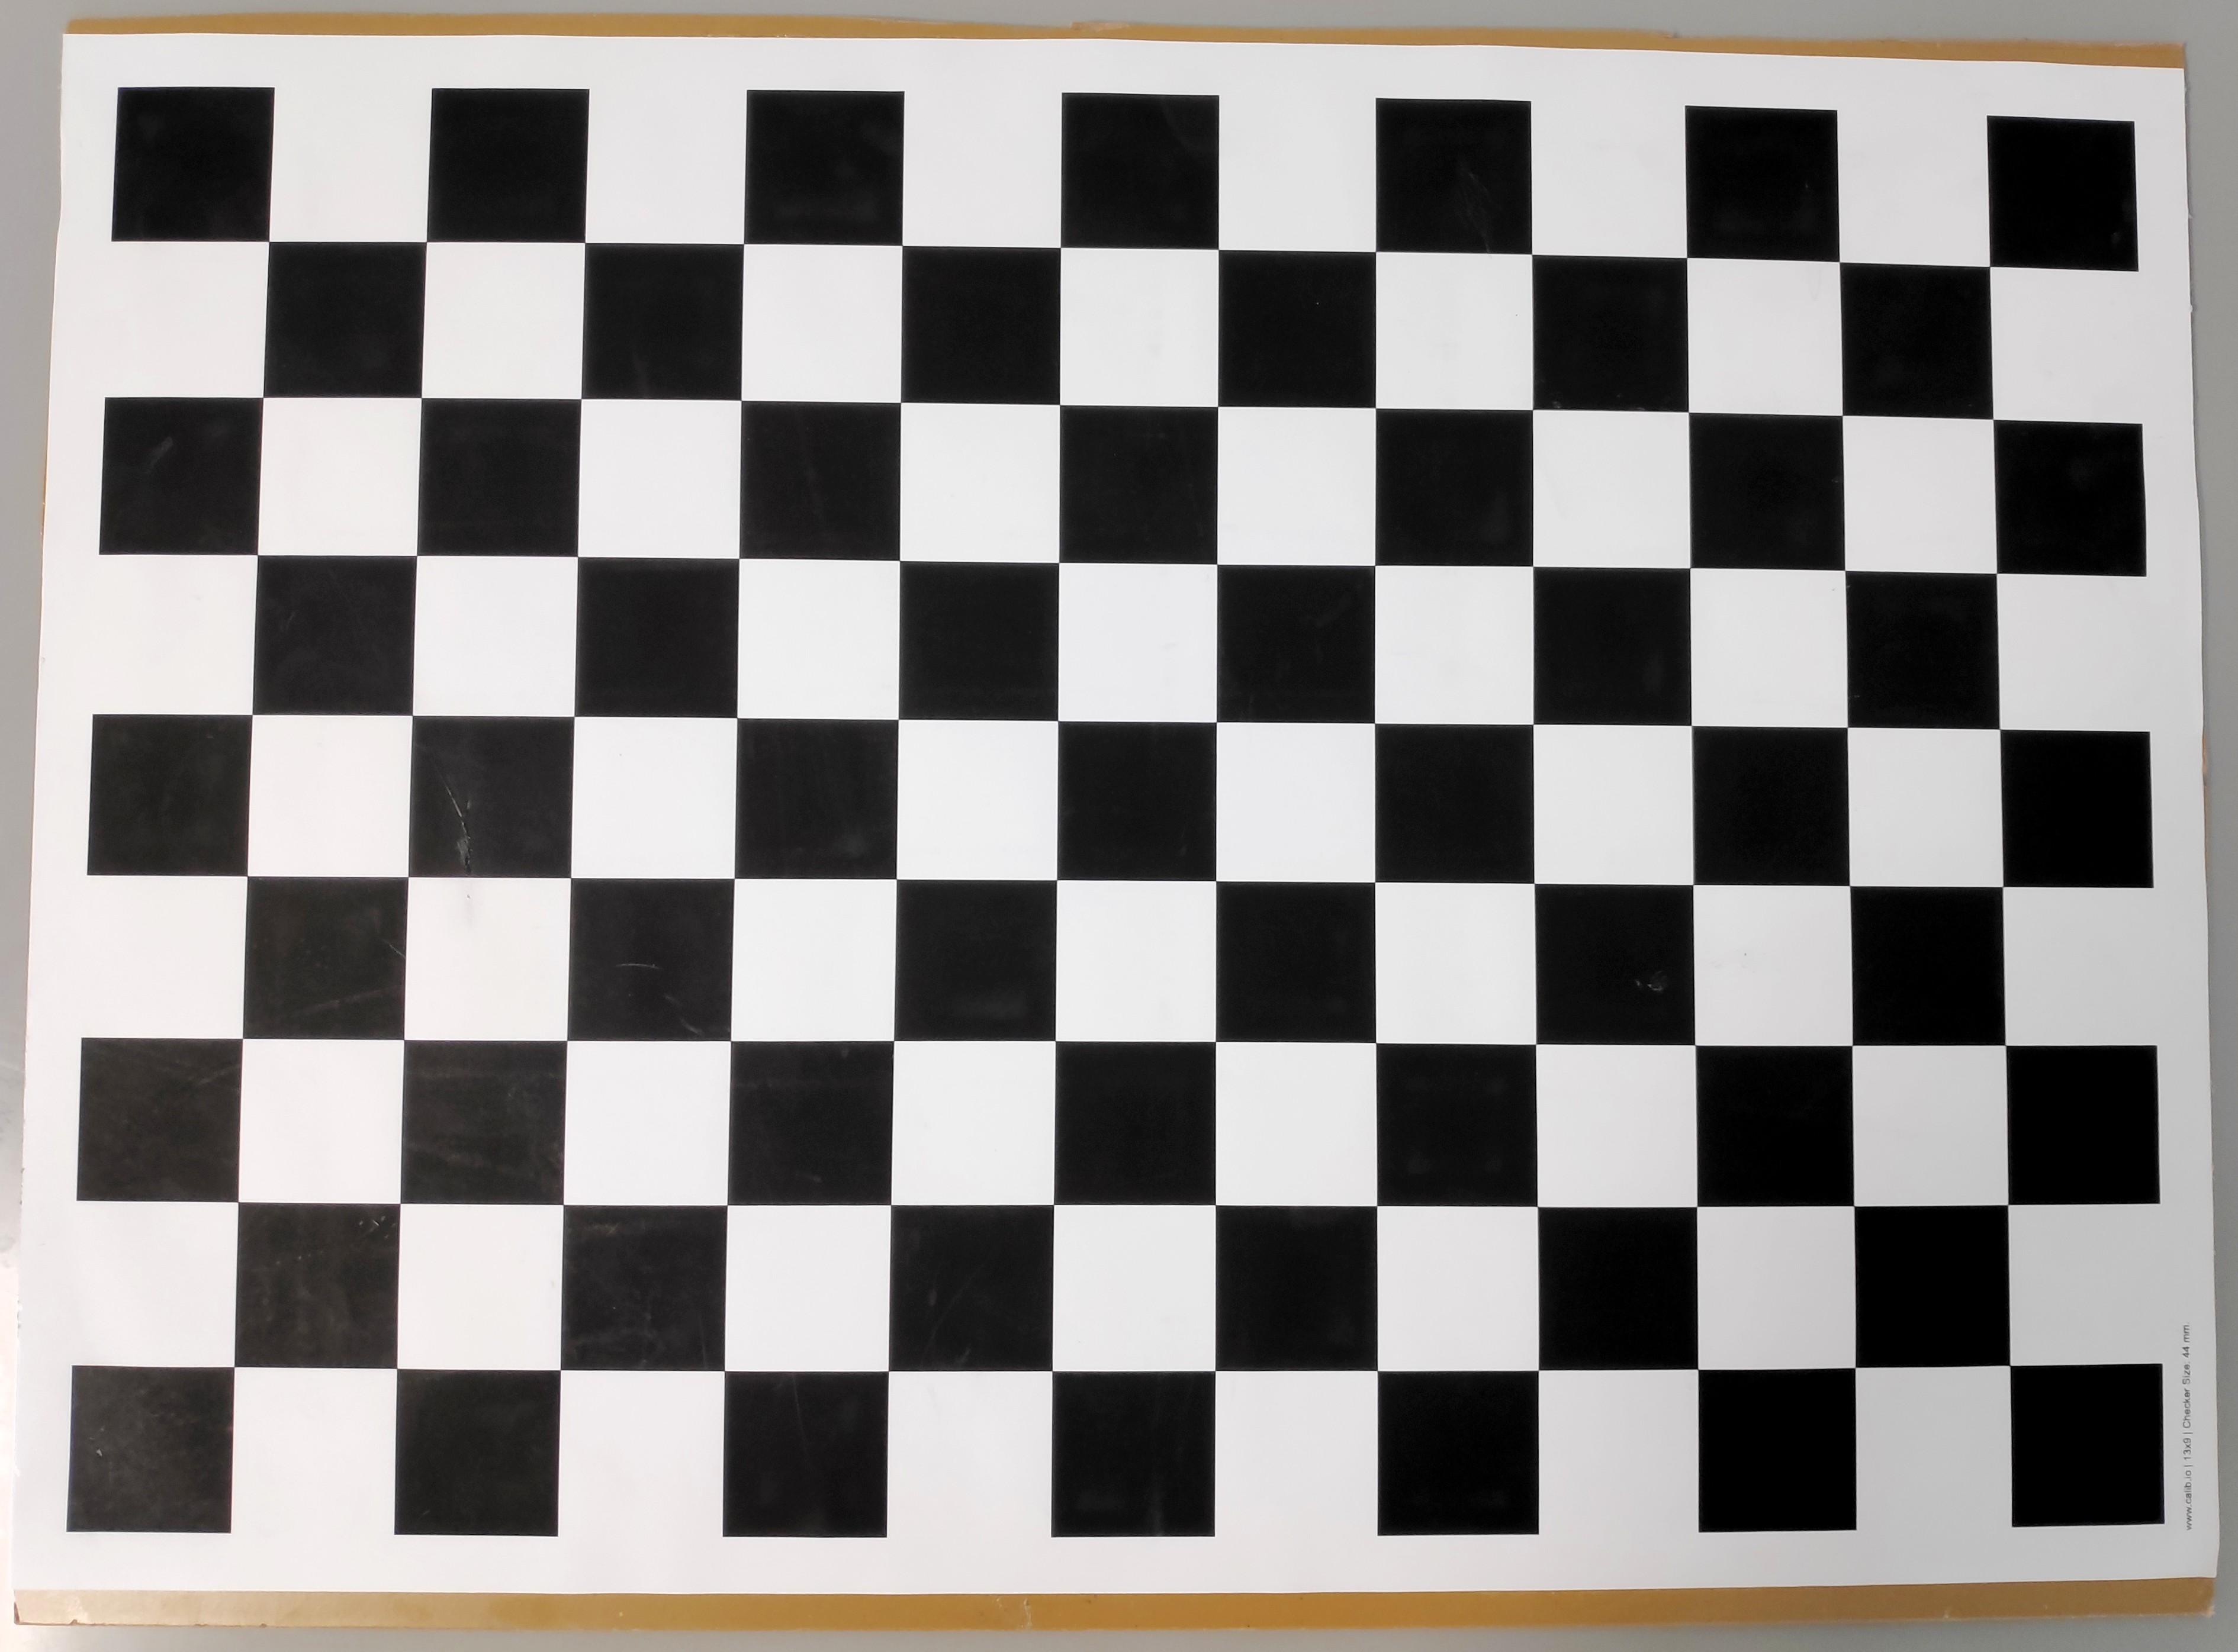
\includegraphics[width=0.5\textwidth]{img/experimental-setup/chessboard.jpg}
	\caption{Chessboard used during camera calibration procedures. The chessboard was laser printed on A2 paper size, in real size, that was then glued to a plywood board.}
	\label{fig:chessboard}
\end{figure}

Calibrating the camera requires that the calibration object to be focused. Therefore, before any proper calibration can be made, focus theory and procedure are given on the next sub-section,~\ref{subsec:calibration:camera-focus}.


\subsection{Camera Focus and \acl{dof}}
\label{subsec:calibration:camera-focus}
Focusing a camera can only be attained for an exact distance from the camera~\cite{Merklinger1993, Photopillers}, measured perpendicularly to the plane of focus, which is the plane containing the \ac{cmos} or \ac{ccd} chip. Therefore, on every image, there is a plane of focus and what actually ``looks focused'' is really just in ``acceptably sharp focus''.

``Acceptably sharp focus'' means that a point in the real world would not result in a point on the image (as happens in precise focus), but in a blurred spot~\cite{Photopillers}. However, if the size of blur is small enough, little to no differences can be perceived and the image is considered to be focused~\cite{Photopillers}. The maximum size at which this blur is not noticed by the viewer (given a specific sensor size, dimension of the viewed photo, viewing distance and acuity of the viewer) is when the \ac{coc} is smaller than the pixel size~\cite{Photopillers, Merklinger1993}.

The first step in focusing an image requires the calculation of the hyperfocal distance, $H$, the distance at which the camera is focused to ensure objects from half of this distance to the infinity are in an ``acceptably sharp focus'' (referred to as just focus, from now on). This distance can be calculated using the equation~\eqref{eq:hyperfocal_distance}, below, where $f$ is the focal length, $F_N$ is the F-number and $c$ the \ac{coc} limit. Hyperfocal near limit is defined as $H_\text{near} = \rfrac{H}{2}$.

\begin{equation}
	\label{eq:hyperfocal_distance}
	H = \frac{f^2}{F_Nc} + f \approx \frac{f^2}{F_Nc} 
\end{equation}

Known the hyperfocal distance, the \acf{dof} can be calculated. \ac{dof} is measured in meters and is obtained by subtracting the farthest and nearest distances at which an object is focused (see Equation~\eqref{eq:dof}), indicating the distance between this two points~\cite{Photopillers, Merklinger1993, mvg_book}. The nearest and farthest points can be calculated using the equations~\eqref{eq:dof-near} and~\eqref{eq:dof-far}, respectively, where $d$ is the target object distance to the camera sensor.

\begin{subequations}
	\label{eq:dof_all}
	\begin{align}
		DoF & = DoF_{far} - DoF_{near} \label{eq:dof} \\
		DoF_{far} & = \frac{H\times d}{H - (d - f)} \label{eq:dof-far} \\
		DoF_{near} & = \frac{H\times d}{H + (d - f)} \label{eq:dof-near} 
	\end{align}
\end{subequations}

Equations~\eqref{eq:dof_all} make it possible to select a desired \acl{dof} for an image that guarantees that all the objects of interest are focused. Taking in consideration that smaller apertures (bigger F-numbers) will increase the exposition time~\cite{Merklinger1993} (since the amount of light illuminating the sensor will be lower), a target distance can be selected with the guarantee that all the objects from the near \ac{dof} point to the far \ac{dof} will be sharp.

Rewriting the Equation~\eqref{eq:dof-near} to calculate the objects distance, giving the minimum distance at the objects must be focused, one gets: %the Equation~\eqref{eq:dof-subject-distance}.

\begin{equation}
	\label{eq:dof-subject-distance}
	d = \frac{(H - f) \cdot DoF_{near}}{H - DoF_{near}}
\end{equation}


\subsection{Camera Calibration Procedure}
For calibration, \ac{opencv} algorithms are used~\cite{opencv_doc}, such as \texttt{calibrateCamera}, \texttt{solvePnP} and \texttt{findChessboardCorners}. These algorithms, the underlying code interconnecting them and a \ac{gui} for performing calibration are available in a \ac{ros} package, \texttt{camera\_calibration} from the \texttt{image\_pipeline} metapackage~\cite{cameraCalibrationRos}, which we use for intrinsic camera calibration.

For calibration, around 50 unique photos are taken for each setup. These images are converted to greyscale, the chessboard corners are detected and the camera intrinsic parameters are computed by the \texttt{camera\_calibration} ROS package. A subset of the calibration images is presented on Figure~\ref{fig:camera-calibration-images}.

\begin{figure}[!ht]
	\centering
	\begin{subfigure}[c]{0.30\textwidth}
		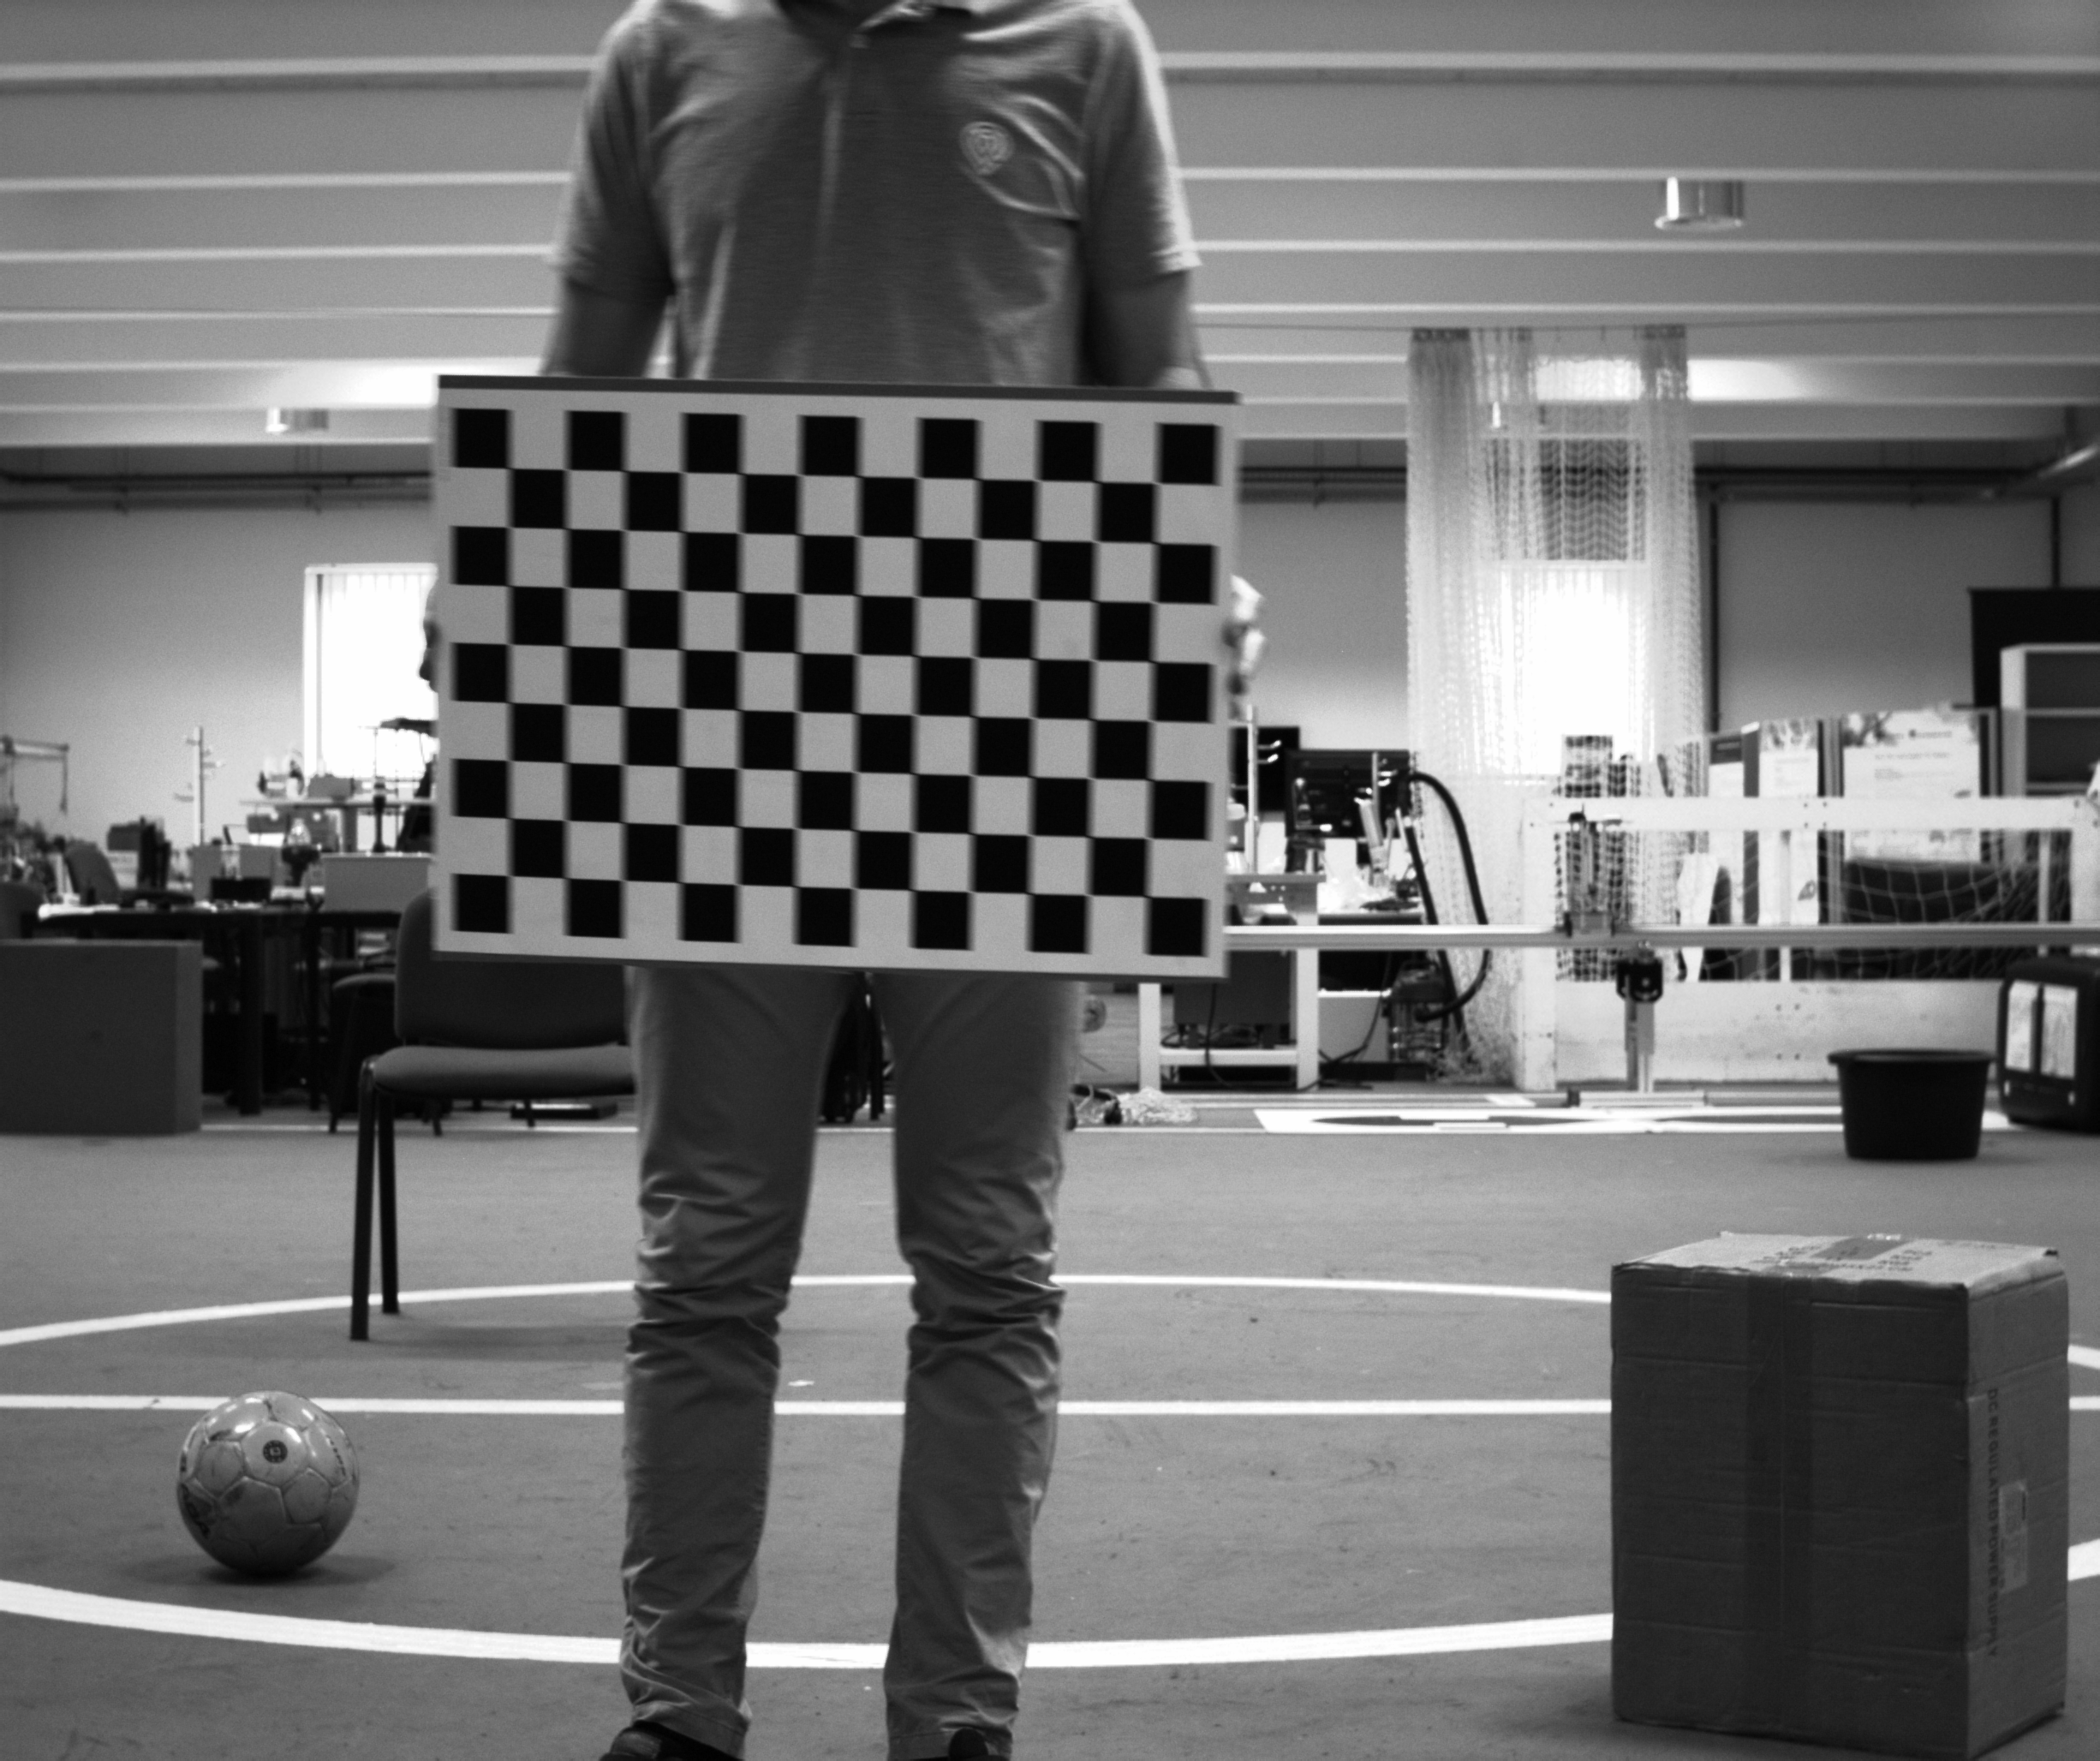
\includegraphics[width=0.9\textwidth]{img/camera-calibration/left-0001.png}
	\end{subfigure}
	\begin{subfigure}[c]{0.30\textwidth}
		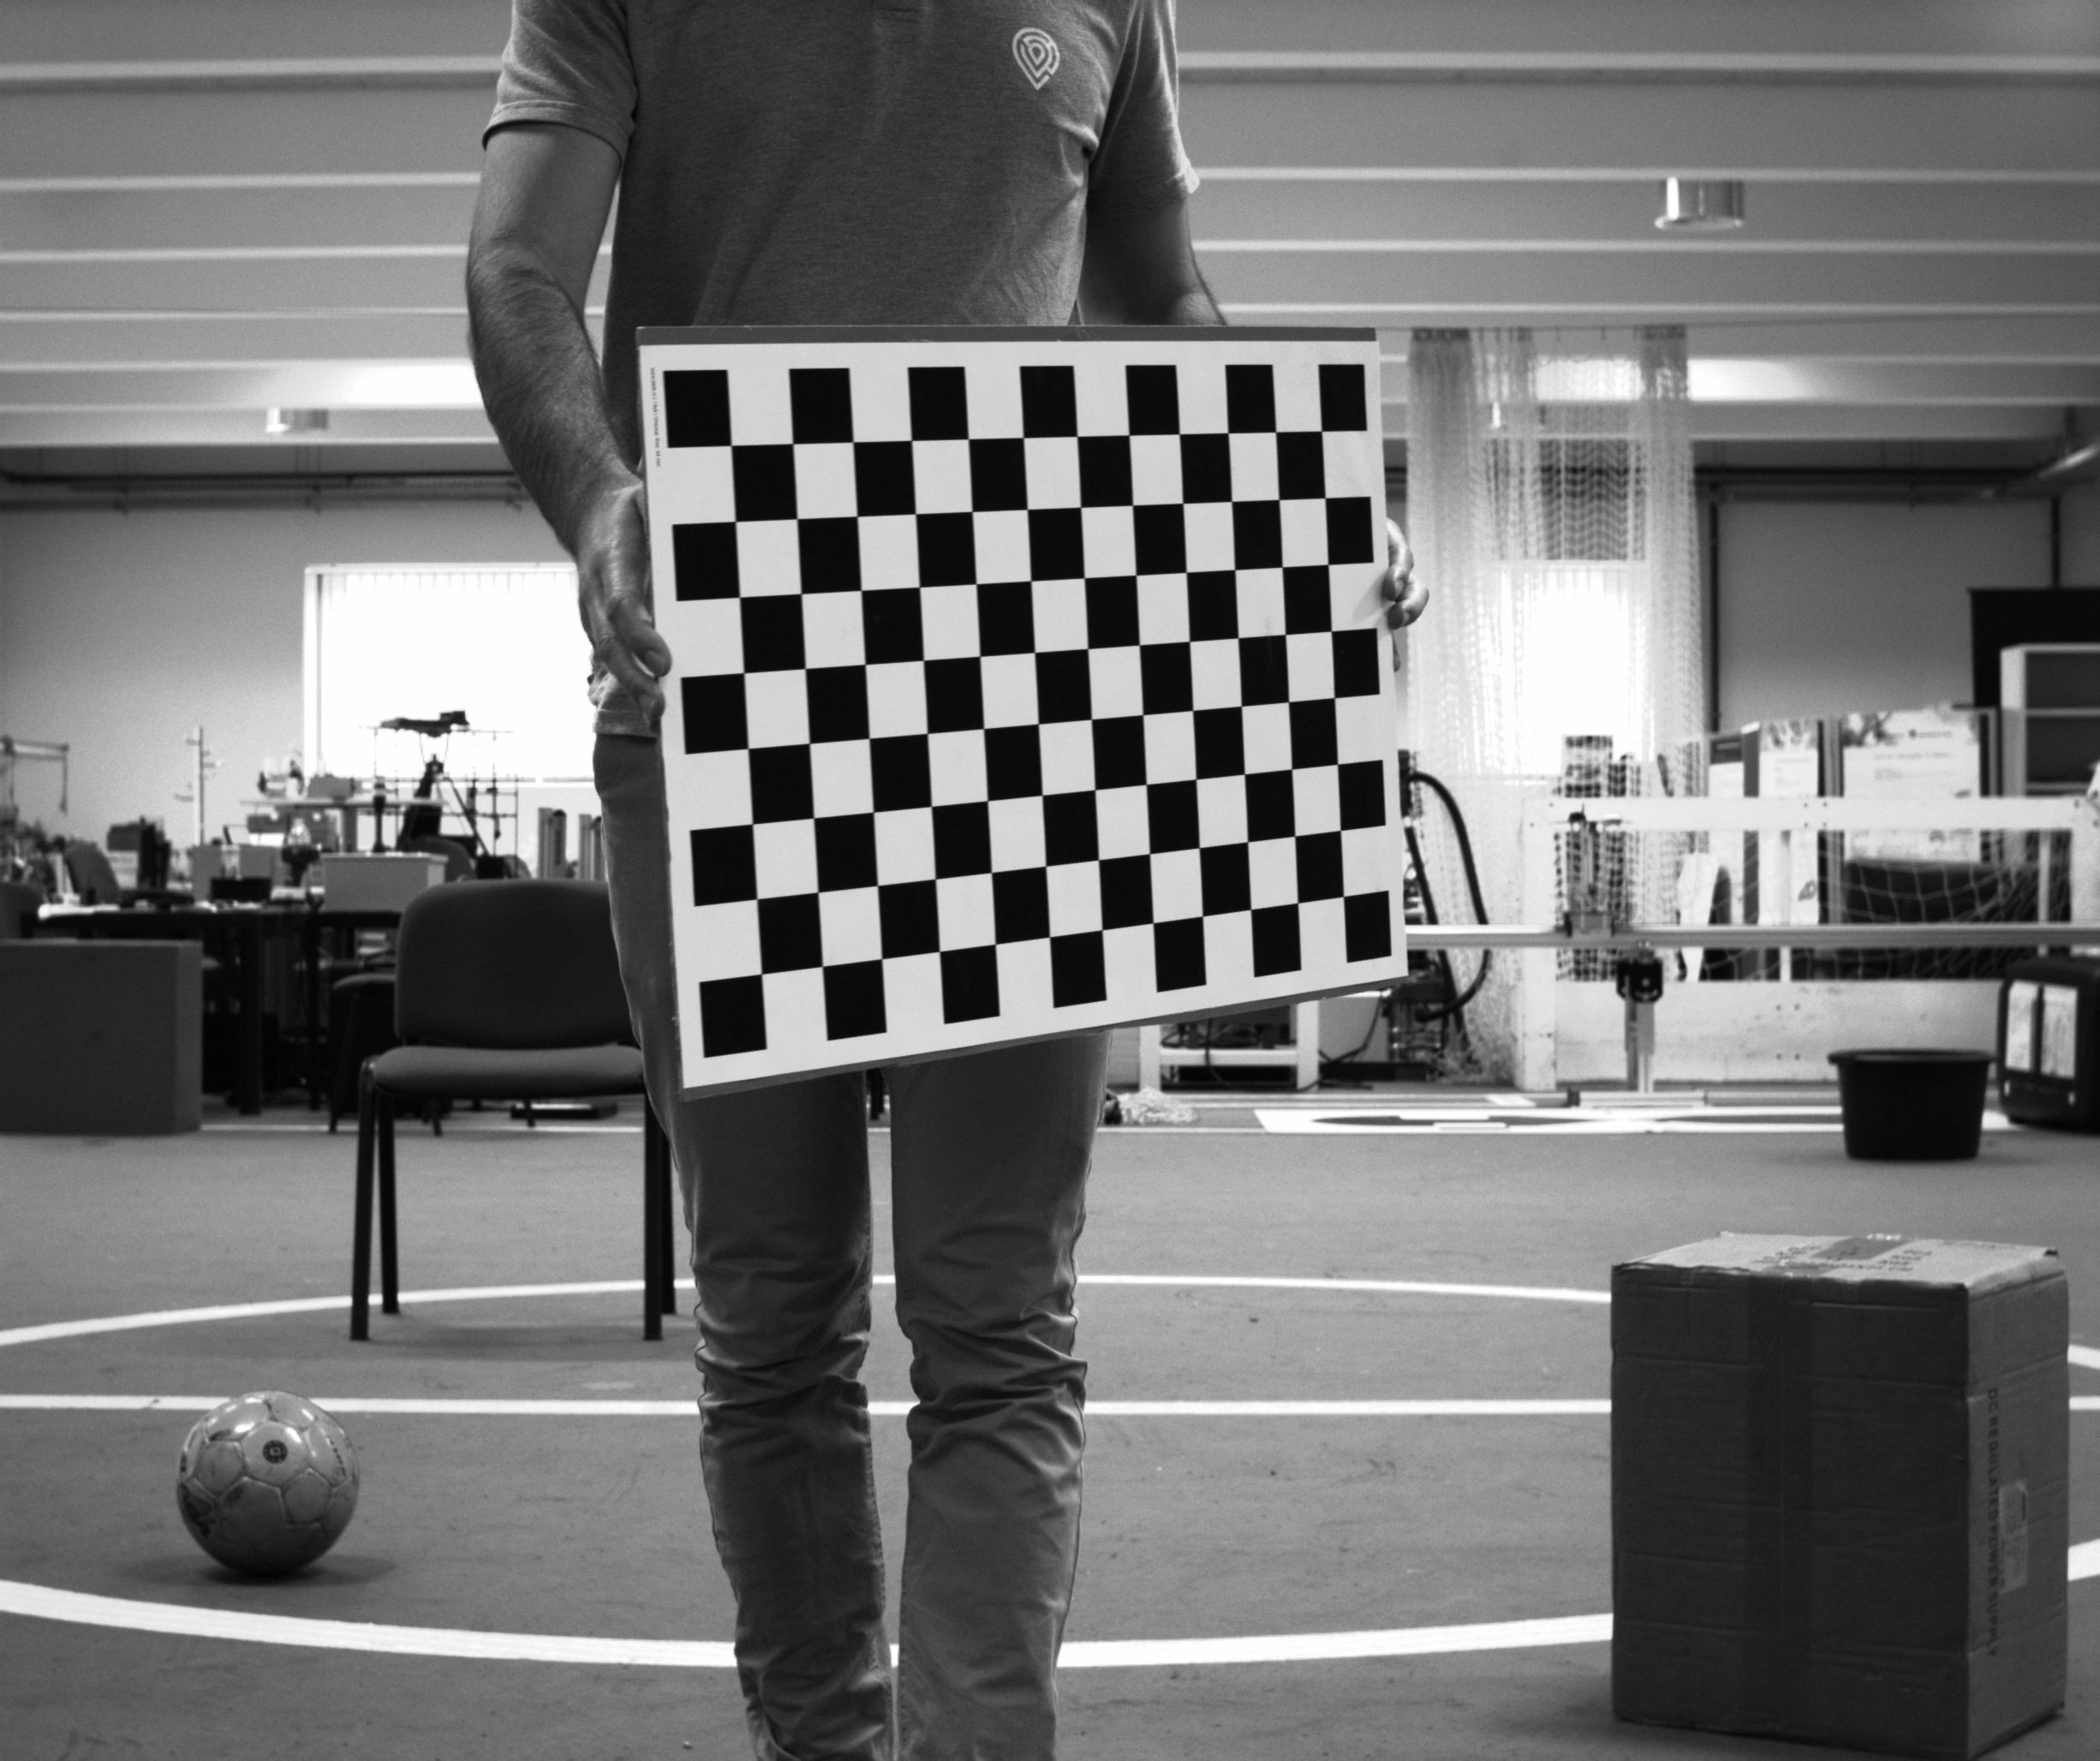
\includegraphics[width=0.9\textwidth]{img/camera-calibration/left-0005.png}
	\end{subfigure}
	\begin{subfigure}[c]{0.30\textwidth}
		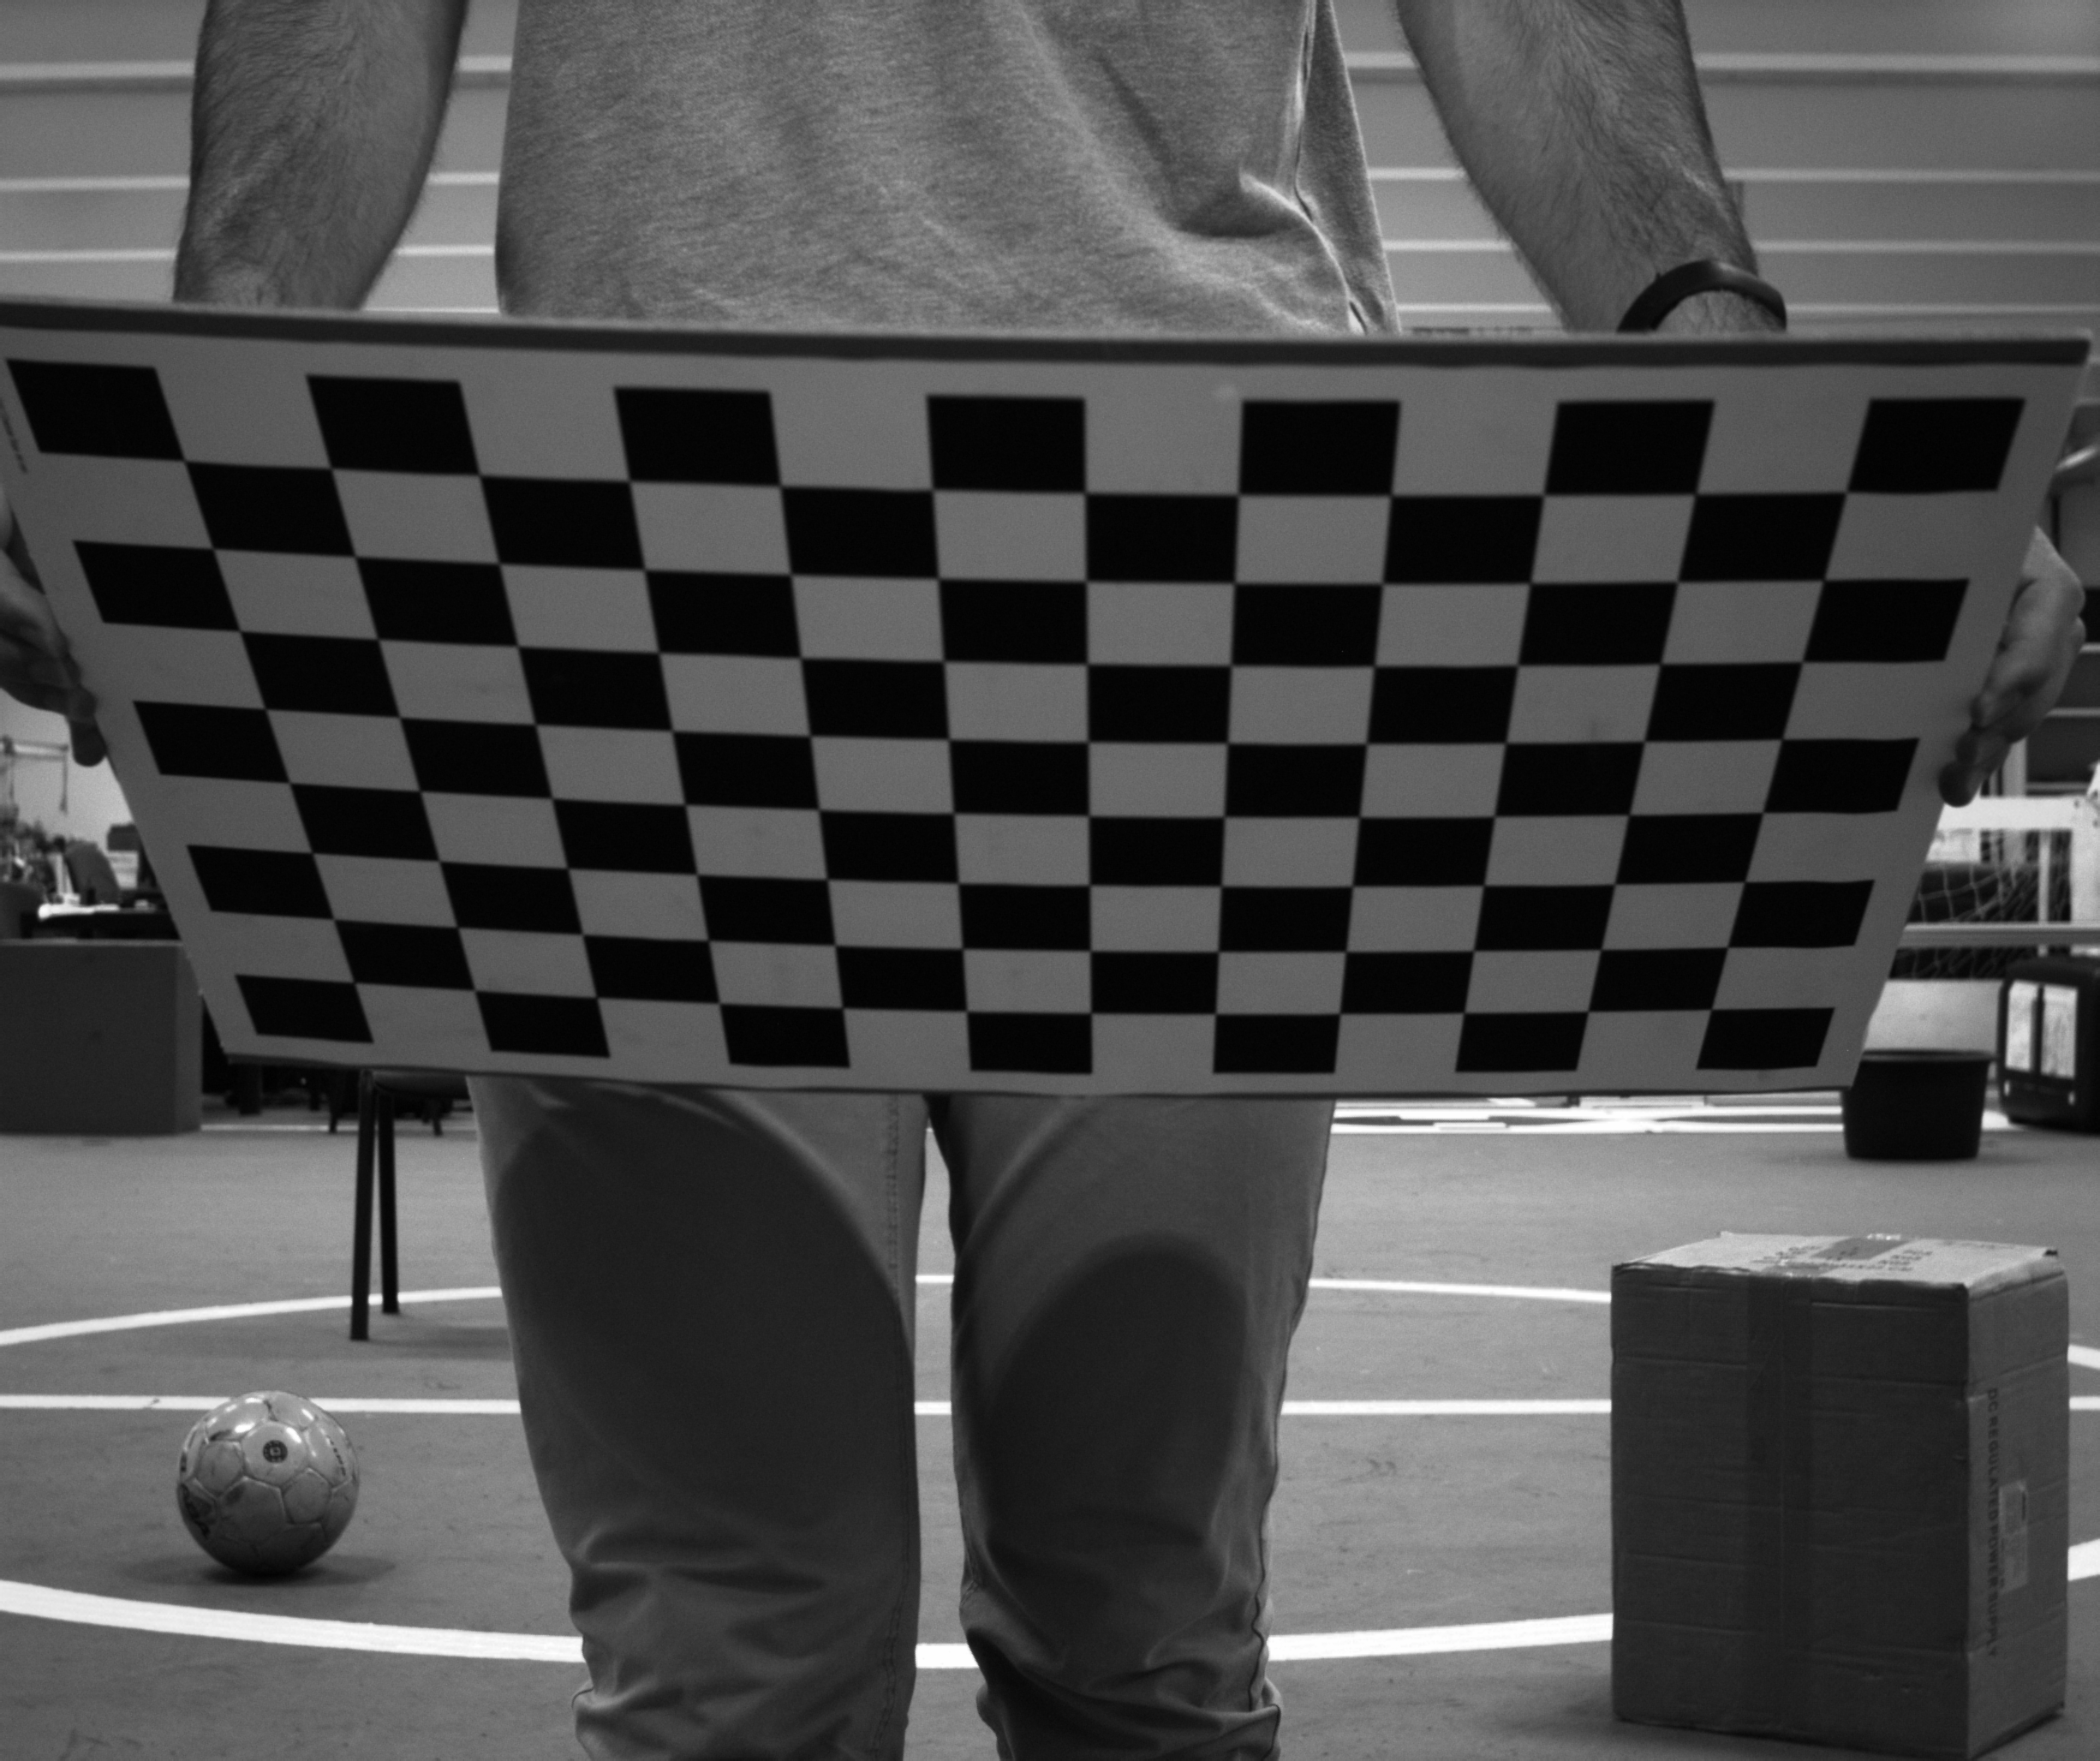
\includegraphics[width=0.9\textwidth]{img/camera-calibration/left-0022.png}
	\end{subfigure}
	\\ 
	\vspace{5mm}
	\begin{subfigure}[c]{0.30\textwidth}
		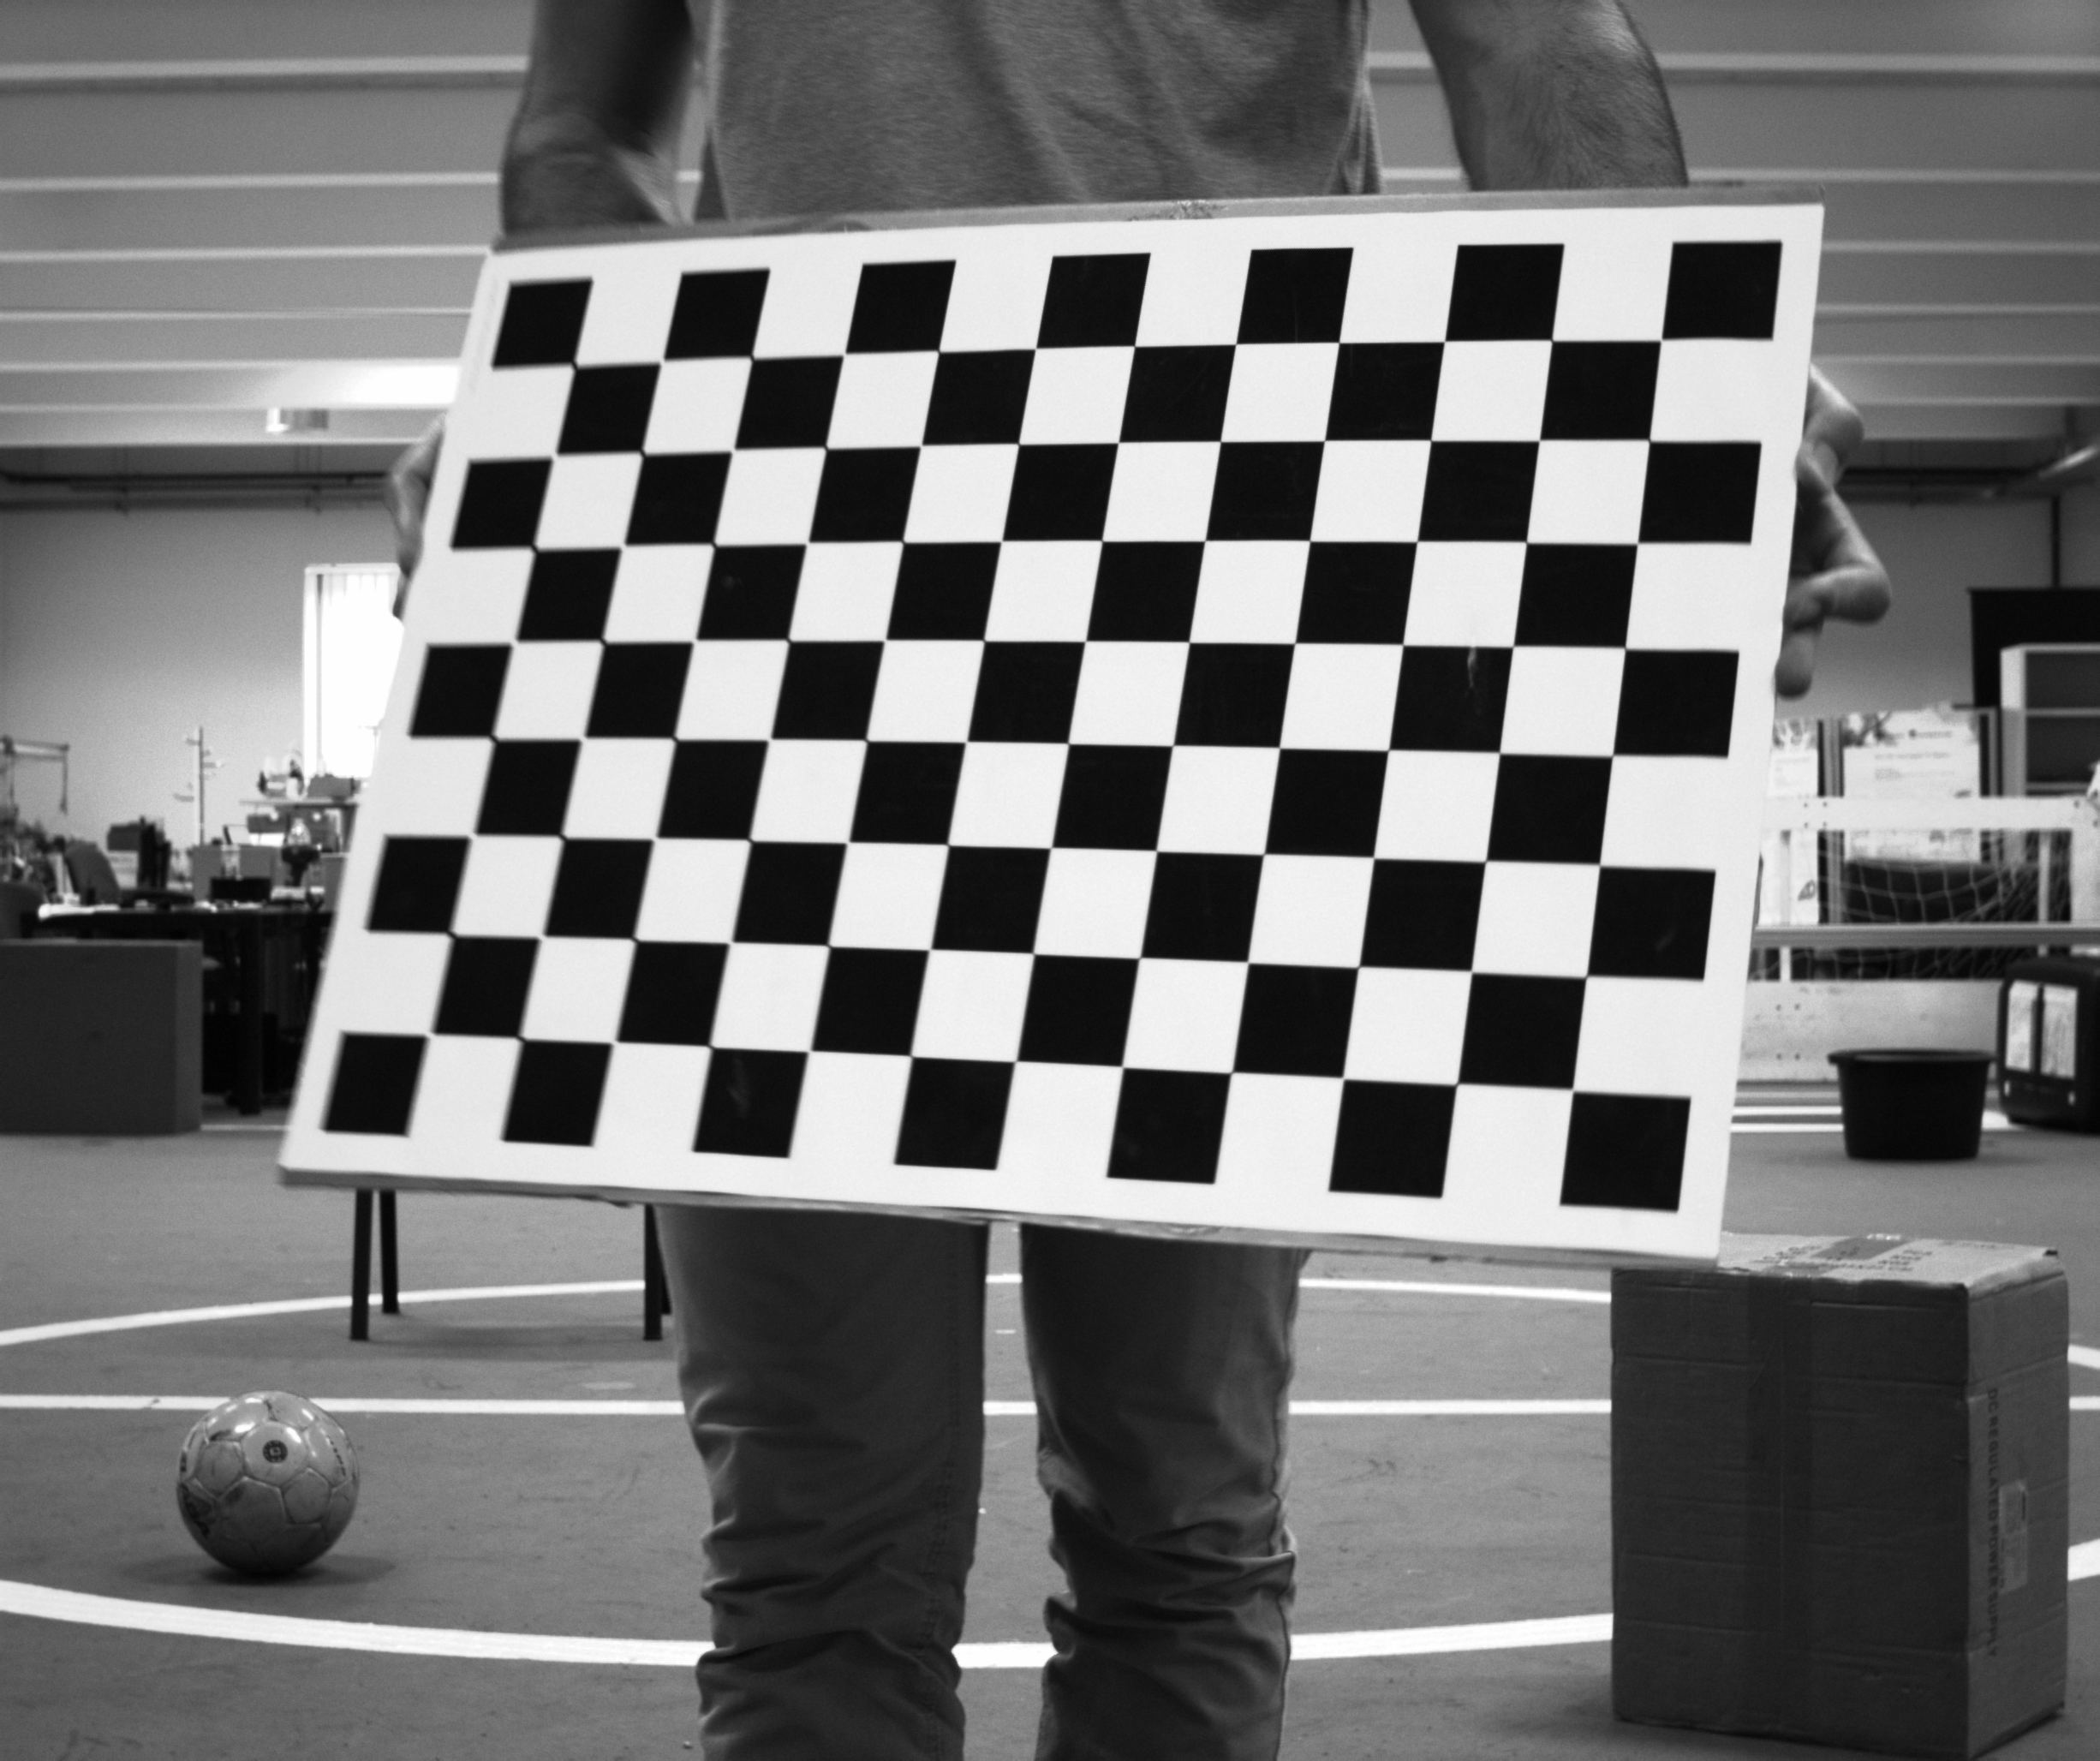
\includegraphics[width=0.9\textwidth]{img/camera-calibration/left-0030.png}
	\end{subfigure}
	\begin{subfigure}[c]{0.30\textwidth}
		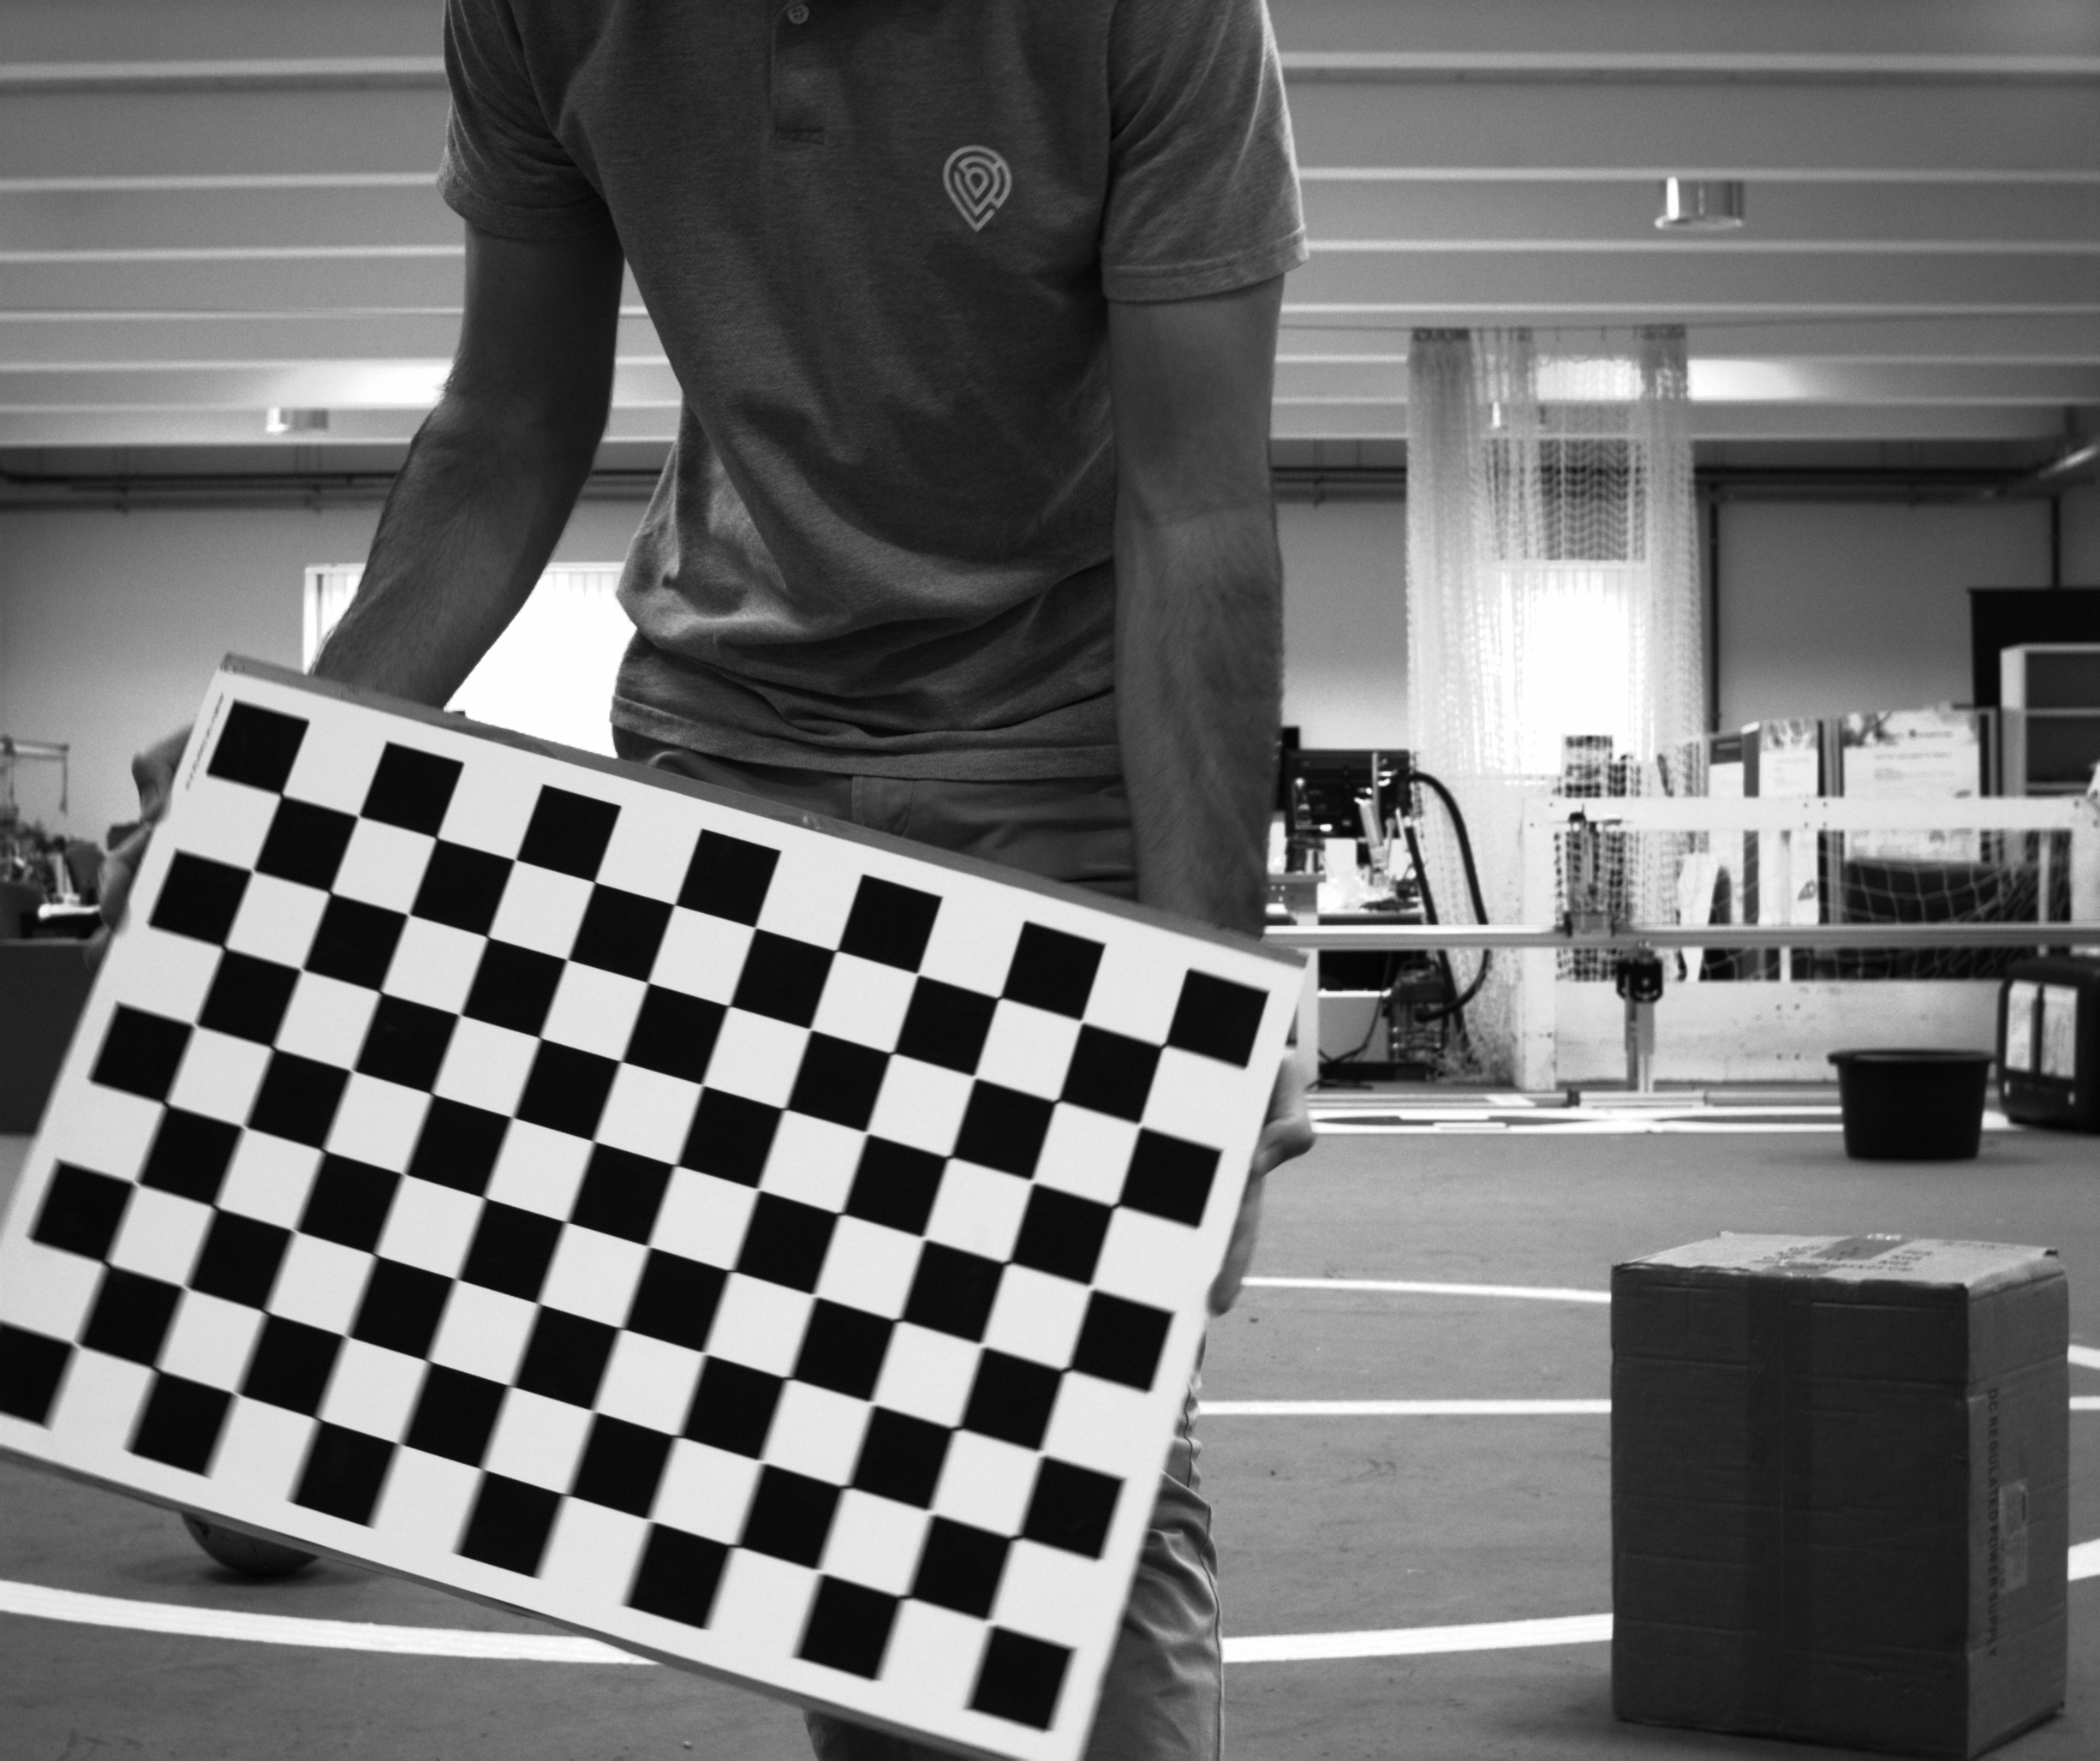
\includegraphics[width=0.9\textwidth]{img/camera-calibration/left-0044.png}
	\end{subfigure}
	\begin{subfigure}[c]{0.30\textwidth}
		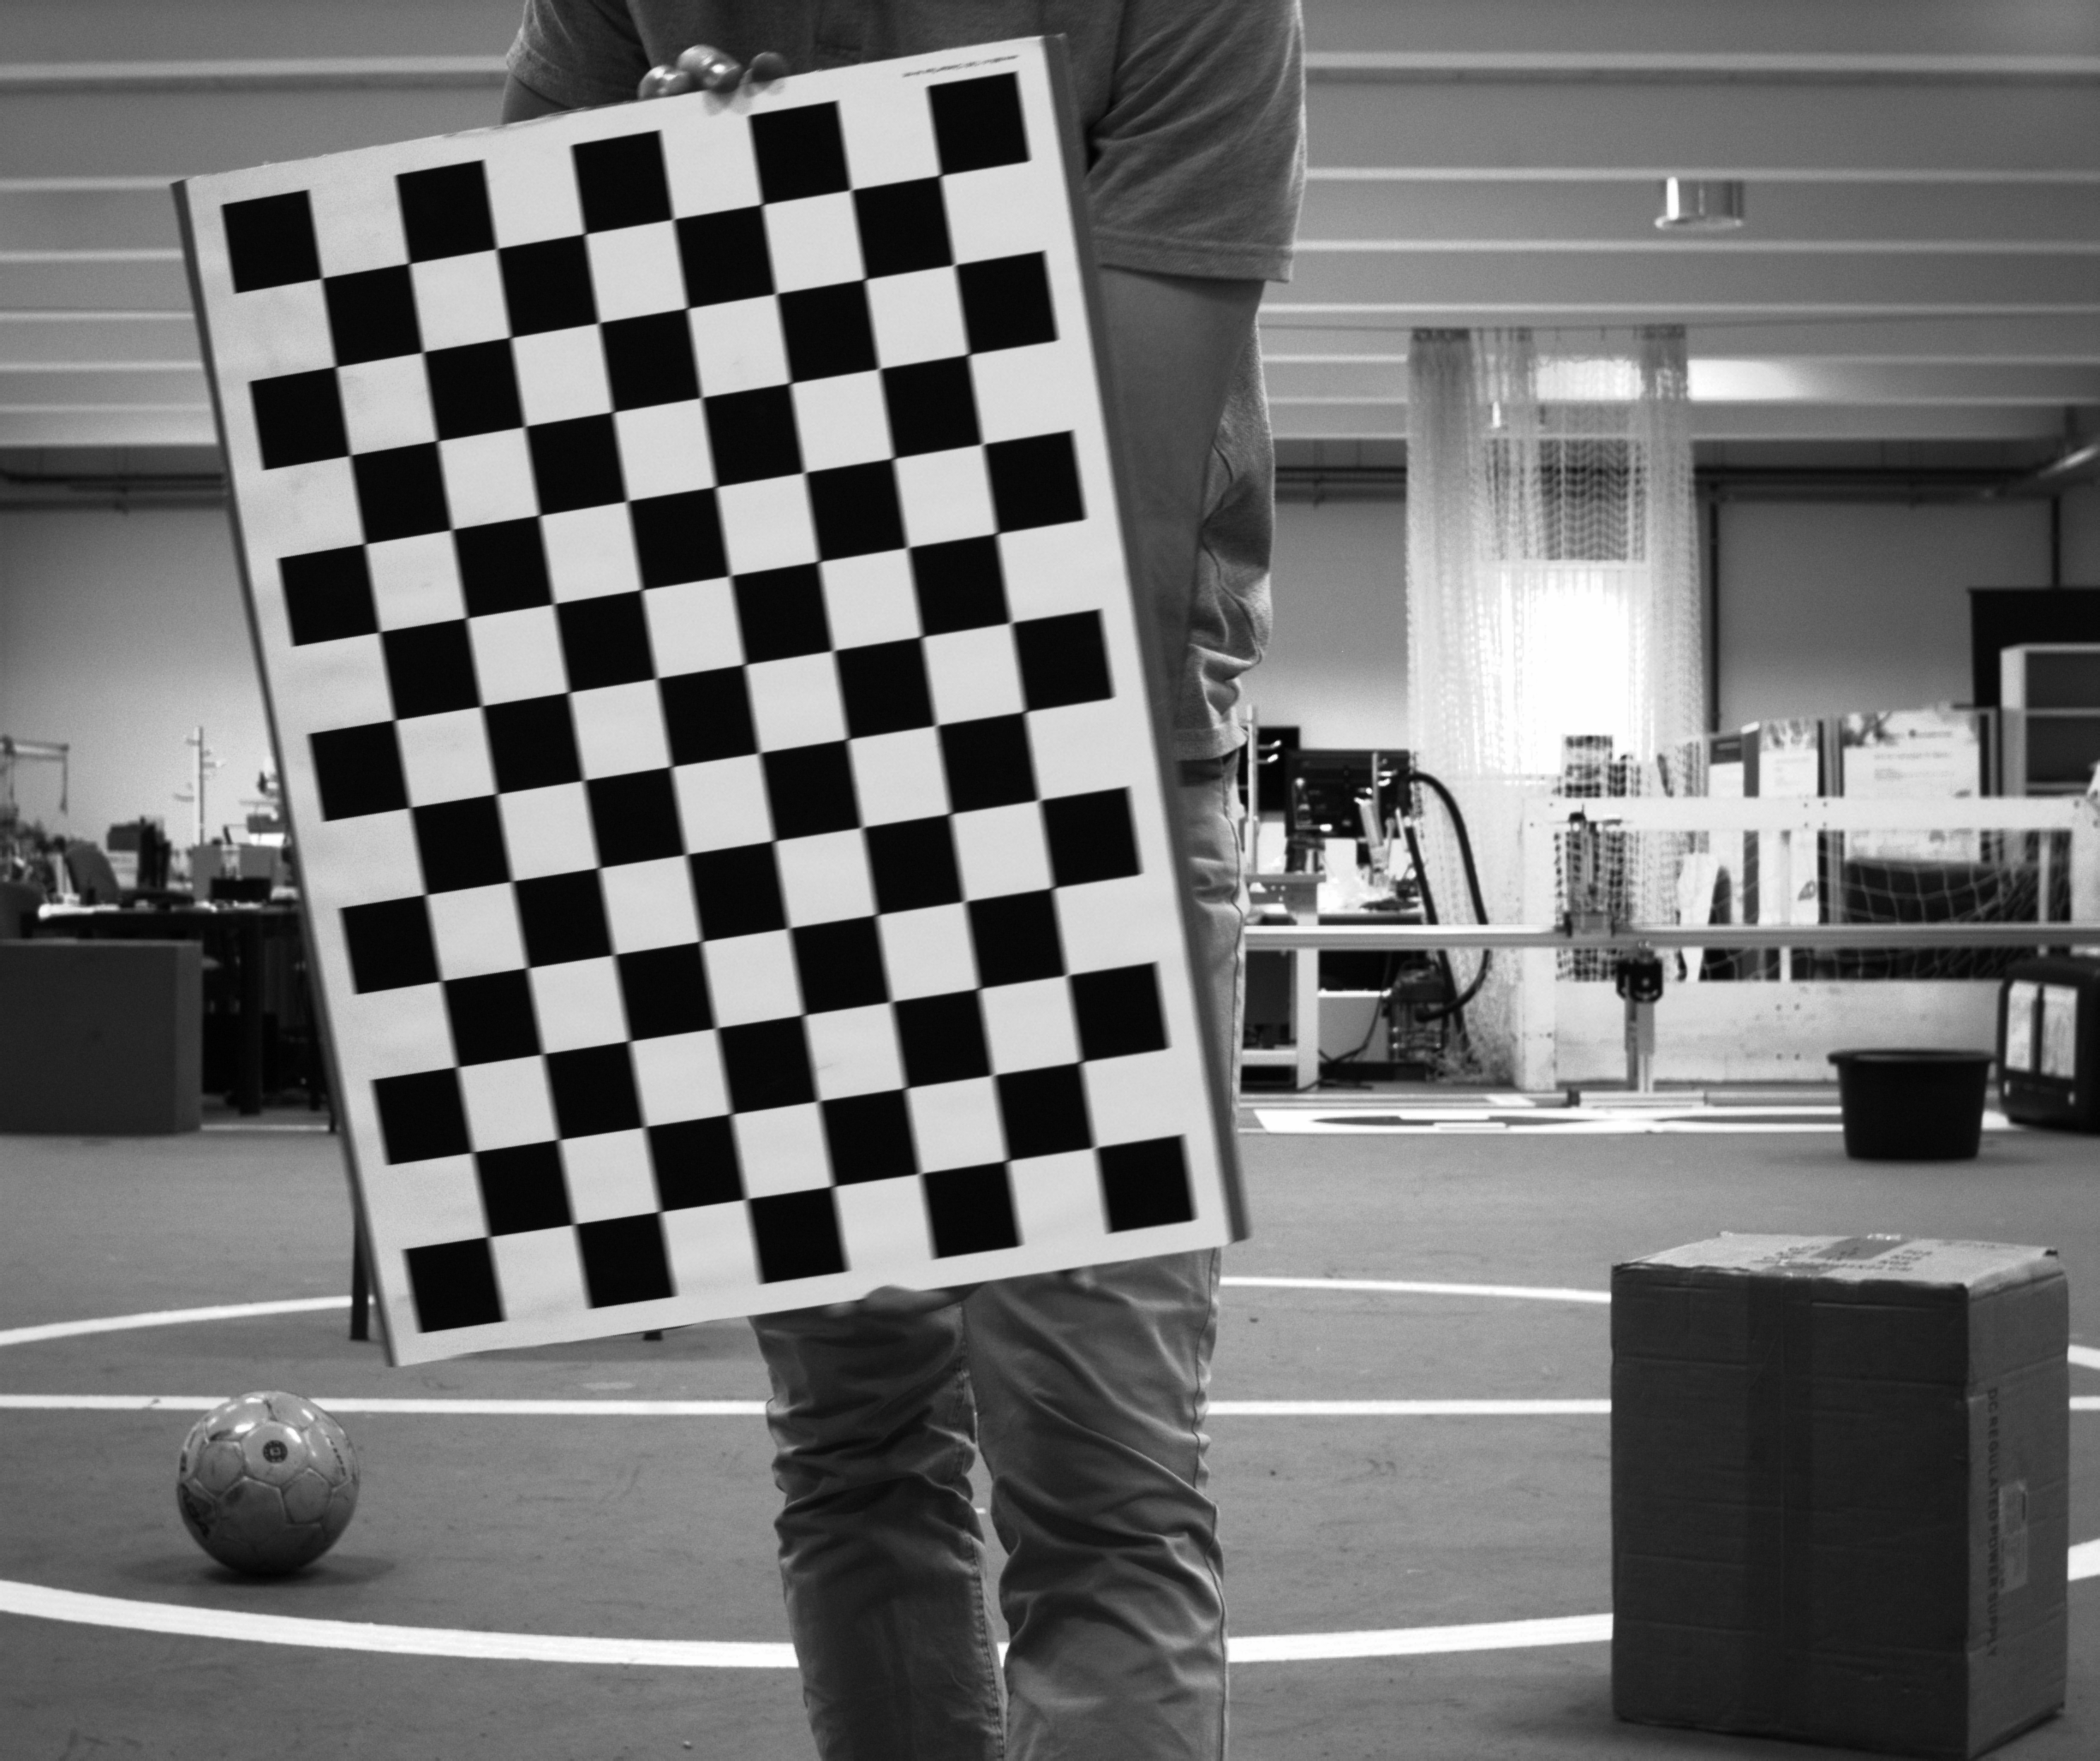
\includegraphics[width=0.9\textwidth]{img/camera-calibration/left-0048.png}
	\end{subfigure}
	
	\caption[Subset of figures used for intrinsic camera calibration.]{Subset of 6 figures used on camera intrinsic calibration. The figures are all on greyscale and for each figure, the chessboard pattern was moved to generate a unique rotational matrix and translation vector in relation to the camera coordinate frame.}
	\label{fig:camera-calibration-images}
\end{figure}

\subsubsection{Frame Rate and Bandwidth concerns}
Despite the straightforwardness of the process, one of the secondary goals of this thesis is to produce a dataset of scenarios on which \ac{lidar} interference is present. Such goal implies that all data must be properly recorded, organized and stored, including calibration data. \ac{ros} provides \texttt{rosbag}, a package for recording and playing back messages exchanged in a \ac{ros} network, which is used to save data on an external hard-drive.

However, preliminary tests with this tool indicate that it cannot save image topics at $9.2$~\ac{fps}. Other tests have shown that $8$~\ac{fps} is the best scenario where \texttt{rosbag} can record data without causing buffer flush due to overrun errors. 

When calibrating the camera, \texttt{camera\_calibration} package drops the frame rate to $\approx 4$~\ac{fps}, because it cannot operate at the desired data flow. If de-Bayerization\footnote{Converting the raw data, stored on a Bayer Filter raw format, to a RGB image} and/or rectification is being applied to the image for saving a pre-processed image, frame rate drops to $\approx 2$~\ac{fps}, since \texttt{image\_proc}, the package responsible for pre-processing the image, cannot process images at the data-rate required for them to be saved on disk, introducing an overhead. Therefore, all images are sent from camera on the raw format \texttt{BayerGB8} and recorded with \texttt{rosbag} in the same format. Note that despite the camera providing  the \texttt{RGB8Packed} color format, the hardware processing required on the camera hardware forces frame rate to be below $8$ \ac{fps}, reason why it was not chosen.

At 8~\ac{fps}, the bandwidth occupied by a 5~\ac{mp} image stream is $8 \cdot 2452 \cdot 2056 \approx \SI[per-mode=symbol]{40}{\mega\byte\per\second}$. Manta's bandwidth limit configuration register was set to a value $25\%$ higher, \SI[per-mode=symbol]{50}{\mega\byte\per\second}, to accommodate other transmissions from the computer to camera and vice-versa. No bandwidth problems were registered, besides occasionally frame drops on the starting or ending of computer processes.

Therefore, for normal operation, Manta \ac{avt} G-504C is set to trigger image capture at a fixed frame rate of $8$~\ac{fps} and when being under an internal calibration procedure, at $4$~\ac{fps}. If better computer hardware has available, internal calibration procedure could be runt at the same frame rate as normal operation, since the bottleneck is on the computer.

However, to ensure the camera runs at the desired number of \ac{fps}, other parameters that affect frame rate must also be managed, such as exposure time.


\subsubsection{Lens Aperture and Exposure Time}
Thorlabs\cp~MVL16M1 lens has several possible apertures: $f/1.4$, $f/2.0$, $f/2.8$, $f/4.0$, $f/8.0$, $f/16.0$. The smaller the F-number\footnote{F-number represents the ratio of the lens' focal length to its effective aperture diameter.}, the bigger the entrance aperture, allowing the camera sensor to be exposed to more light within the same time interval. More light indicates that exposure time can be reduced, since the sensor receives the same amount of light in less time to produce a sharp image.

However, decreasing the F-number reduces the Hyperfocal distance (see Equation~\eqref{eq:hyperfocal_distance}), which in turn reduces the \acf{dof}. A trade-off must then be addressed between \ac{dof} and F-number, which implies that three parameters must be fine-tuned: \ac{dof}, exposure time and image frame rate, since they are all interconnected. As stated above, a maximum \ac{fps} is desirable, but due to recording constraints of the \texttt{rosbag} package, $8$~\ac{fps} is the target image frame-rate. This implies that, at $8$\ac{fps}, the camera must never take more than \SI{125}{\milli\second} since the start of exposure to the broadcast of the message on the Ethernet network, which means that exposure time must be shorter. Through experimental analysis, the maximum exposure which seems to not disturb the desired frame rate is \SI{100}{\milli\second}. 

The F-number needs to be adjusted not only to ensure the requirements of the exposure time are met and to maximize \acl{dof}, but also to ensure that exposure can be increased or decrease to accommodate the daylight intensity variations. Considering a maximum exposure time of \SI{100}{\milli\second}, only aperture values greater than $f/4.0$ result on a sharp image under those constraints. To maximize the \ac{dof}, the smaller F-number should be chosen, since \ac{dof} and the F-number are inversely proportional. Therefore, with such constrains, our experimental setup uses an F-number of $f/4.0$ and an exposure time that varies between \SIrange{80}{100}{\milli\second} during daylight.

\subsubsection{\acl{dof} and calibration object}
\label{subsec:calibration:dof-and-calibration-object}
Solving Equation~\eqref{eq:hyperfocal_distance} and replacing its result on Equation~\eqref{eq:dof-subject-distance}, we can obtain $d$, the object distance at which the camera must be focused. The object to be focused is the calibrating pattern and the $DoF_{near}$ limit is select to be the distance at which the calibration pattern fills the camera~\ac{fov}. The calculations can be seen in Equation~\eqref{eq:hyperfocal-and-dof-values}.

\begin{subequations}
	\label{eq:hyperfocal-and-dof-values}
	\begin{align}
		H & = \frac{16mm^2}{4.0 \cdot 0.020mm} + 16mm  = 3.216 m \label{eq:hyperfocal-distance-value} \\
		\vspace{25mm}
		d & = \frac{(3.216 - 16mm) \cdot 1.405}{3.216 - 1.405} = 2.49m \label{eq:dof-subject-distance-value}
	\end{align}
\end{subequations}

After focusing the camera, the \texttt{cameracalibrator.py} node is run, using the command below. Note that the chessboard patterns argument is $12\times 8$ and not $13 \times 9$, because the \texttt{size} argument refers to the number of interior corners, not number of squares on the chessboard.


\begin{verbatim}
    rosrun camera_calibration cameracalibrator.py --size 12x8 --square 0.044  
        monocular:=/camera image:=/camera/image_raw
\end{verbatim}


After the \ac{gui} registers all the images, the calculation of calibration parameters can be initiated and the parameters are saved on a \textit{.ost} file for later use and/or sent the configuration to the camera. 

To interact with the Manta AVT G-504C, \texttt{avt\_vimba\_camera} \ac{ros} package~\cite{AVTROSdriver}, which depends on VIMBA GigE SDK, is used to operate the camera. It also provides compatibility with the \texttt{camera\_calibration} package, crucial for a straightforward calibration process.

\subsection{Camera Calibration Results}
The \ac{ros} node diagrams can be seen on Figure~\ref{fig:camera-calibration-rosgraph}. On sub-Figure~\ref{fig:camera-calibration-bag-rosgraph}, the nodes and topics for the calibration procedure using the data published by the \texttt{rosbag} tool. On sub-Figure~\ref{fig:camera-calibration-avt-rosgraph}, the nodes and topics for the calibration procedure using the data directly from the driver are shown. 


\begin{figure}[H]
	\vspace{5mm}
	\centering
	\begin{subfigure}[c]{0.8\textwidth}
		\centering
		\def\svgwidth{\columnwidth}
		\graphicspath{{img/camera-calibration/}}
		\includesvg{img/camera-calibration/bag-rosgraph-print}
		%
\includegraphics[width=0.8\textwidth]{img/camera-calibration/bag-rosgraph.png}
		\caption{\ac{ros} node graph for the camera calibration procedure using the \texttt{rosbag} tool. \texttt{RosbagPlayer} is the node that plays back the data stored on the bag file.}
		\label{fig:camera-calibration-bag-rosgraph}
	\end{subfigure}
	\vspace{5mm} \\ 
	\begin{subfigure}[c]{0.8\textwidth}
		\centering
		\def\svgwidth{\columnwidth}
		\graphicspath{{img/camera-calibration/}}
		\includesvg{img/camera-calibration/avt-rosgraph-print}
		%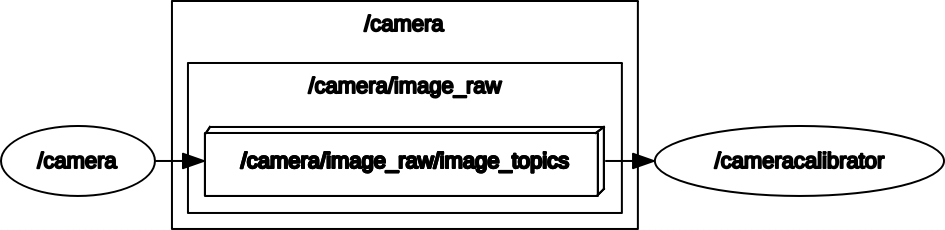
\includegraphics[width=0.8\textwidth]{img/camera-calibration/avt-rosgraph.png}		
		\caption{\ac{ros} node for the camera calibration procedure using the \ac{avt} Vimba \ac{ros} driver. \texttt{camera} node refers to \ac{ros} node that wraps the \ac{avt} Vimba driver.}
		\label{fig:camera-calibration-avt-rosgraph}
	\end{subfigure}
	\caption[Camera calibration \acs{ros} node diagram.]{Camera Calibration node graph for \ac{ros} nodes. \texttt{cameracalibrator} is the node responsible for computing the intrinsic camera calibration parameters, either if they are (\subref{fig:camera-calibration-bag-rosgraph}) being replayed using \texttt{rosbag}; (\subref{fig:camera-calibration-avt-rosgraph}) or coming directly from the camera driver.}
	\label{fig:camera-calibration-rosgraph}
\end{figure}

The camera was calibrated daily whenever experimental measures were taken. The calibration for one of these days is shown below, where $\mathbf{K}$ is the camera intrinsic parameters' matrix, $\mathbf{D}$ is the lens distortion coefficients vector and $\mathbf{P}$ the camera projective matrix. %on Equation~\eqref{eq:camera-calibration-results}.

\begin{subequations}
	\label{eq:camera-calibration-results}
	\begin{align}
		\mathbf{K} & = 
		\begin{bmatrix}
			4595.944192 & 0.0         &  1313.9194945 \\
			0.0         & 4593.466666 &  952.554450 \\
			0.0         & 0.0         &  1.0
		\end{bmatrix} \nonumber \\
		\mathbf{D} & = 
		\begin{bmatrix}
			-0.304037 & 1.364428 &  -0.005705 & 0.003330 & 0.0
		\end{bmatrix} \nonumber \\
		\mathbf{P} & = 
		\begin{bmatrix}
			4529.381836 & 0.0         & 1318.010062 & 0.0 \\
			0.0         & 4534.939941 & 947.167736  & 0.0 \\
			0.0         & 0.0         & 1.0         & 0.0 
		\end{bmatrix}
		\nonumber
	\end{align}
\end{subequations}

	

\section{\ac{lidar} Intrinsic Calibration}
\label{sec:calibration:lidar}
Unlike a camera, \acp{lidar} do not possess a typical calibration procedure. For Velodyne VLP-16 reflectivity measurements are factory calibrated, in a procedure described in~\cite{vlp16} and a \ac{xml} file is provided with the \ac{lidar}, containing corrections for the \ac{lidar} operating parameters.

This file must be converted to a more suitable format, \acs{yaml}~\footnote{\acs{yaml} is an acronym for \acl{yaml}. The author chose not to follow the norm of expanding acronyms' inline due to acronym recursive nature, to facilitate reading.}, which is \ac{ros} default and can be loaded by the Velodyne \ac{ros} driver package, \texttt{velodyne}, for correction of the \ac{lidar} measurements. After observing the point cloud with test objects such as boxes and walls, \ac{lidar} calibration is observed to be accurate and no further calibration procedures were undertaken.

\section{Camera and \ac{lidar} Extrinsic Calibration}
\label{sec:calibration:extrinsic}
Calibrating the camera and \ac{lidar}, as explained in Section~\ref{subsec:sota:camera-intrinisc-calibration}, requires determining the rigid body transform between the reference frames of the two sensors. A rigid body transform, also known as a Euclidean Isometry since it preserves the distance between points~\cite{mvg_book}, has 6 degrees of freedom, that can be represented by a translation and a rotation vector.

Due to the ambiguity of the rotation vector and its variety of interpretations: (1) it can represent one of twelve Euler angles notation, angle axis notation, amongst others; (2) this notation is normally replaced by the unambiguous rotation matrix (see Equation~\eqref{eq:camera_transform_full} for an example) or a quaternion. Such representations are also free from gimbal lock, a mathematical limitation of the vector representation, that can cause one rotation axis ``locking'' on another, resulting on their rotation no longer being independent of the other, removing one degree of freedom and degenerating into a two-dimensional rotational space. For more details on gimbal lock and other singularities see~\cite{mvg_book, Slabaugh, camera_models}.

In this thesis, the preferred notation is a quaternion, which is also adopted by \ac{ros}~\cite{Foote2014}. A quaternion is a mathematical object belonging to $\mathbb{R}^4$, that has a vector (or imaginary) part and a scalar (or real) part. Its representation is denoted on Equation~\eqref{eq:quaternion-notation}, where $\mathbf{i}$, $\mathbf{j}$ and $\mathbf{k}$ are the normalized unit vectors of the $x$, $y$ and $z$ axis, respectively; and $w$ is the scalar part. More information on quaternions can be found on~\cite{mvg_book}.

\begin{equation}
	\label{eq:quaternion-notation}
	q = (x\mathbf{i}, y\mathbf{j}, z\mathbf{k}, w)
\end{equation}

\subsection{Calibration Method}
\label{subsec:calibration:calibration-method}
Given the nature of the sensors: a camera image is two-dimensional and the \ac{lidar} data is tridimensional; the extrinsic calibration needs to consider the projective geometry and its transformations on the camera. Revisiting Equation~\eqref{eq:jointRotationTranslationTransform}, our goal is to determine the joint rotation and translation matrix that allows the conversion of coordinates from the \ac{lidar} to the camera frame. To account for projective geometry, Equation~\eqref{eq:camera_transform_full} must be considered when establishing 3D points to image pixels correspondences.

The method implemented to calibrate the camera and \ac{lidar} is inspired by Scaramuzza's\etal~\cite{Scaramuzza} and Brabec's~\cite{brabec2014} work. The method proposed consists on manually selecting the correspondences between image pixels and 3D points on the \ac{lidar} point cloud. If a single synchronized frame from the camera and \ac{lidar} is used, one can consider the scene as static, and therefore, the joint rotation and translation matrix present in Equation~\eqref{eq:camera_transform_full} is actually the same as the matrix present on Equation~\eqref{eq:jointRotationTranslationTransform}. 

Such considerations are only possible due to the camera using a global shutter instead of rolling shutter. In the former, the image is acquired in a single shot and all the points ``have the same timestamps''. In the latter, each row of the image is acquired one after another, iteratively, therefore, ``having different timestamps''. If a rolling shutter camera was used, for a single image, the \ac{lidar} point cloud could not have been considered static and the delays on the camera shutter and \ac{lidar} rotation would have to be taken into account when calibrating and fusing the data between the two. An exception to the latter is if the \ac{lidar} and camera position is static and the scene is also static.

Since the intrinsic calibration matrix is already obtained by the method described on Section~\ref{sec:calibration:camera}, and the correspondences are selected by the user, the only remaining unknown is the joint rotation and translation matrix. Also, since this method ``reuses'' the equations that are the basis for intrinsic camera calibration, it can also ``reuse'', with some constraints and modifications, the same algorithms~\cite{opencv_doc}, such as \texttt{solvePnP}, which determines the joint rotation and translation matrix that converts world points to camera pixels.


\subsection{Implementation}
To extrinsically calibrate the camera and \ac{lidar}, a multi-node network approach was followed, which can be seen on Figure~\ref{fig:extrinsic-calibration-rosgraph}, on Appendix~\ref{appendix:appendix-diagrams}. Using \ac{opencv} and \ac{pcl}, two visualizers were encapsulated under \ac{ros} nodes written in C++, that subscribe camera and \ac{lidar} messages, respectively. The point cloud visualizer, \texttt{PCL\_Viewer\_with\_Pose}, receives the point cloud data from the \texttt{rosbag} player or the \texttt{velodyne} driver and publishes the coordinates of the selected point and the viewer pose. \texttt{Image\_Visualizer} publishes the pixels selected by the user, but requires the de-Bayering and conversion to RGB of the raw image using the \texttt{image\_proc} package. Despite being wrapped in \ac{ros}, each of the visualizers provides standalone callbacks, that support ``frame freezing'' for correspondences selection.

Another node, \texttt{rigid\_transform\_computation} is responsible for listening to messages containing the selected pixels and points, registering their correspondences. This node  instantiates two \ac{ros} services servers, that can be called asynchronously: one for computing the rigid body transform and another to save the correspondences selected on a \ac{csv} file, for later usage. 

%\begin{figure}[!ht]
%	\centering
%	\def\svgwidth{\columnwidth}
%	\graphicspath{{img/calibration/}}
%	\includesvg{img/calibration/extrinsic-calibration-rosgraph-print}
%	\caption{\ac{ros} node graph for the extrinsic calibration. The nodes are represented in  ellipses and the topics between them in rectangles. Rosbag Player is responsible reproducing the recorded topics.}
%	\label{fig:extrinsic-calibration-rosgraph}
%\end{figure}


The algorithm implemented to compute the 6 degrees of freedom rigid body transformation uses \ac{opencv} \texttt{solvePnP}, which gives the intrinsic camera parameters and the manually selected correspondences between the object points (3D points from \ac{lidar}). It can also compute the rotation and translation vectors. For solving the \ac{pnp} problem, several algorithms can be used: Levenberg-Marquardt~\cite{Levenberg1943}, Effective~\ac{pnp}~\cite{Lepetit2009}, Perspective-Three-Point~\cite{Gao2003}, Direct-Least-Squares~\cite{Hesch2011} or Exhaustive Linearization — Uncalibrated \ac{pnp}~\cite{Penate-Sanchez2013a}. The \ac{ros} node implemented provides an argument to select the desired algorithm to be applied to solve the \ac{pnp} problem.

After resolving the \ac{pnp} with one of the methods above, Rodrigues' algorithm is used to convert the \ac{opencv} rotation vector to a rotation matrix~\cite{Dai2015}, which is then used to derive the quaternion. Combining the quaternion with the translation vector, a static transform is published to the \ac{ros} network, which can be used to convert and fuse data from the camera coordinate frame to the \ac{lidar} and vice-versa.

An additional \ac{ros} node is also created to compute and publish the rigid body transformation from pre-selected correspondences. It loads the correspondences between the 3D points and image pixels from the \ac{csv} file, the camera intrinsic parameters from an \acs{yaml} file. Using the same algorithms as \texttt{rigid\_transform\_computation}, it computes the rigid body transform and publishes it to the \ac{ros} network using \ac{ros} static transformation.


\subsection{Calibration Result}
\label{subsec:calibration:extrinsic-results}
To ease the calibration process, a \ac{ros} launch file is created. A launch file is written in \ac{xml} and provides instructions to \ac{ros} master node on how to run all the necessary nodes to implement a desired functionality. On this case, \texttt{rigid\_transform\_computation.launch}, launches the two visualizers (image and point cloud) and the node responsible for listening to the selected correspondences. 

Several tests were performed with the possible algorithms for solving \ac{pnp}. Since for the version of \ac{opencv} used, $3.2.0$, the Direct-Least-Squares and Uncalibrated \ac{pnp} methods are unstable~\cite{opencv_doc}, with only the Levenberg-Marquardt, Perspective-Three-Point and Effective~\ac{pnp} were tested. 

Although the planar chessboard used for intrinsic camera calibration was present during the extrinsic calibration, the algorithm implemented does not require the usage of a calibration object. For calibration, 6 points were selected in the point cloud and 6 pixels on the image: four of them correspond to the corners of the chessboard and two to a background object. The selected correspondences can be seen in Figure~\ref{fig:calibration-correspondences}: sub Figure~(\subref{fig:extrinsic-calibration-correspondences:camera}) shows the selected pixels on the image, marked with red crosses; sub Figure~(\subref{fig:extrinsic-calibration-correspondences:lidar}) shows the selected 3D points on the point cloud, marked as red spheres.


\begin{figure}[H]
	\centering
	\begin{subfigure}[c]{0.39\textwidth}
		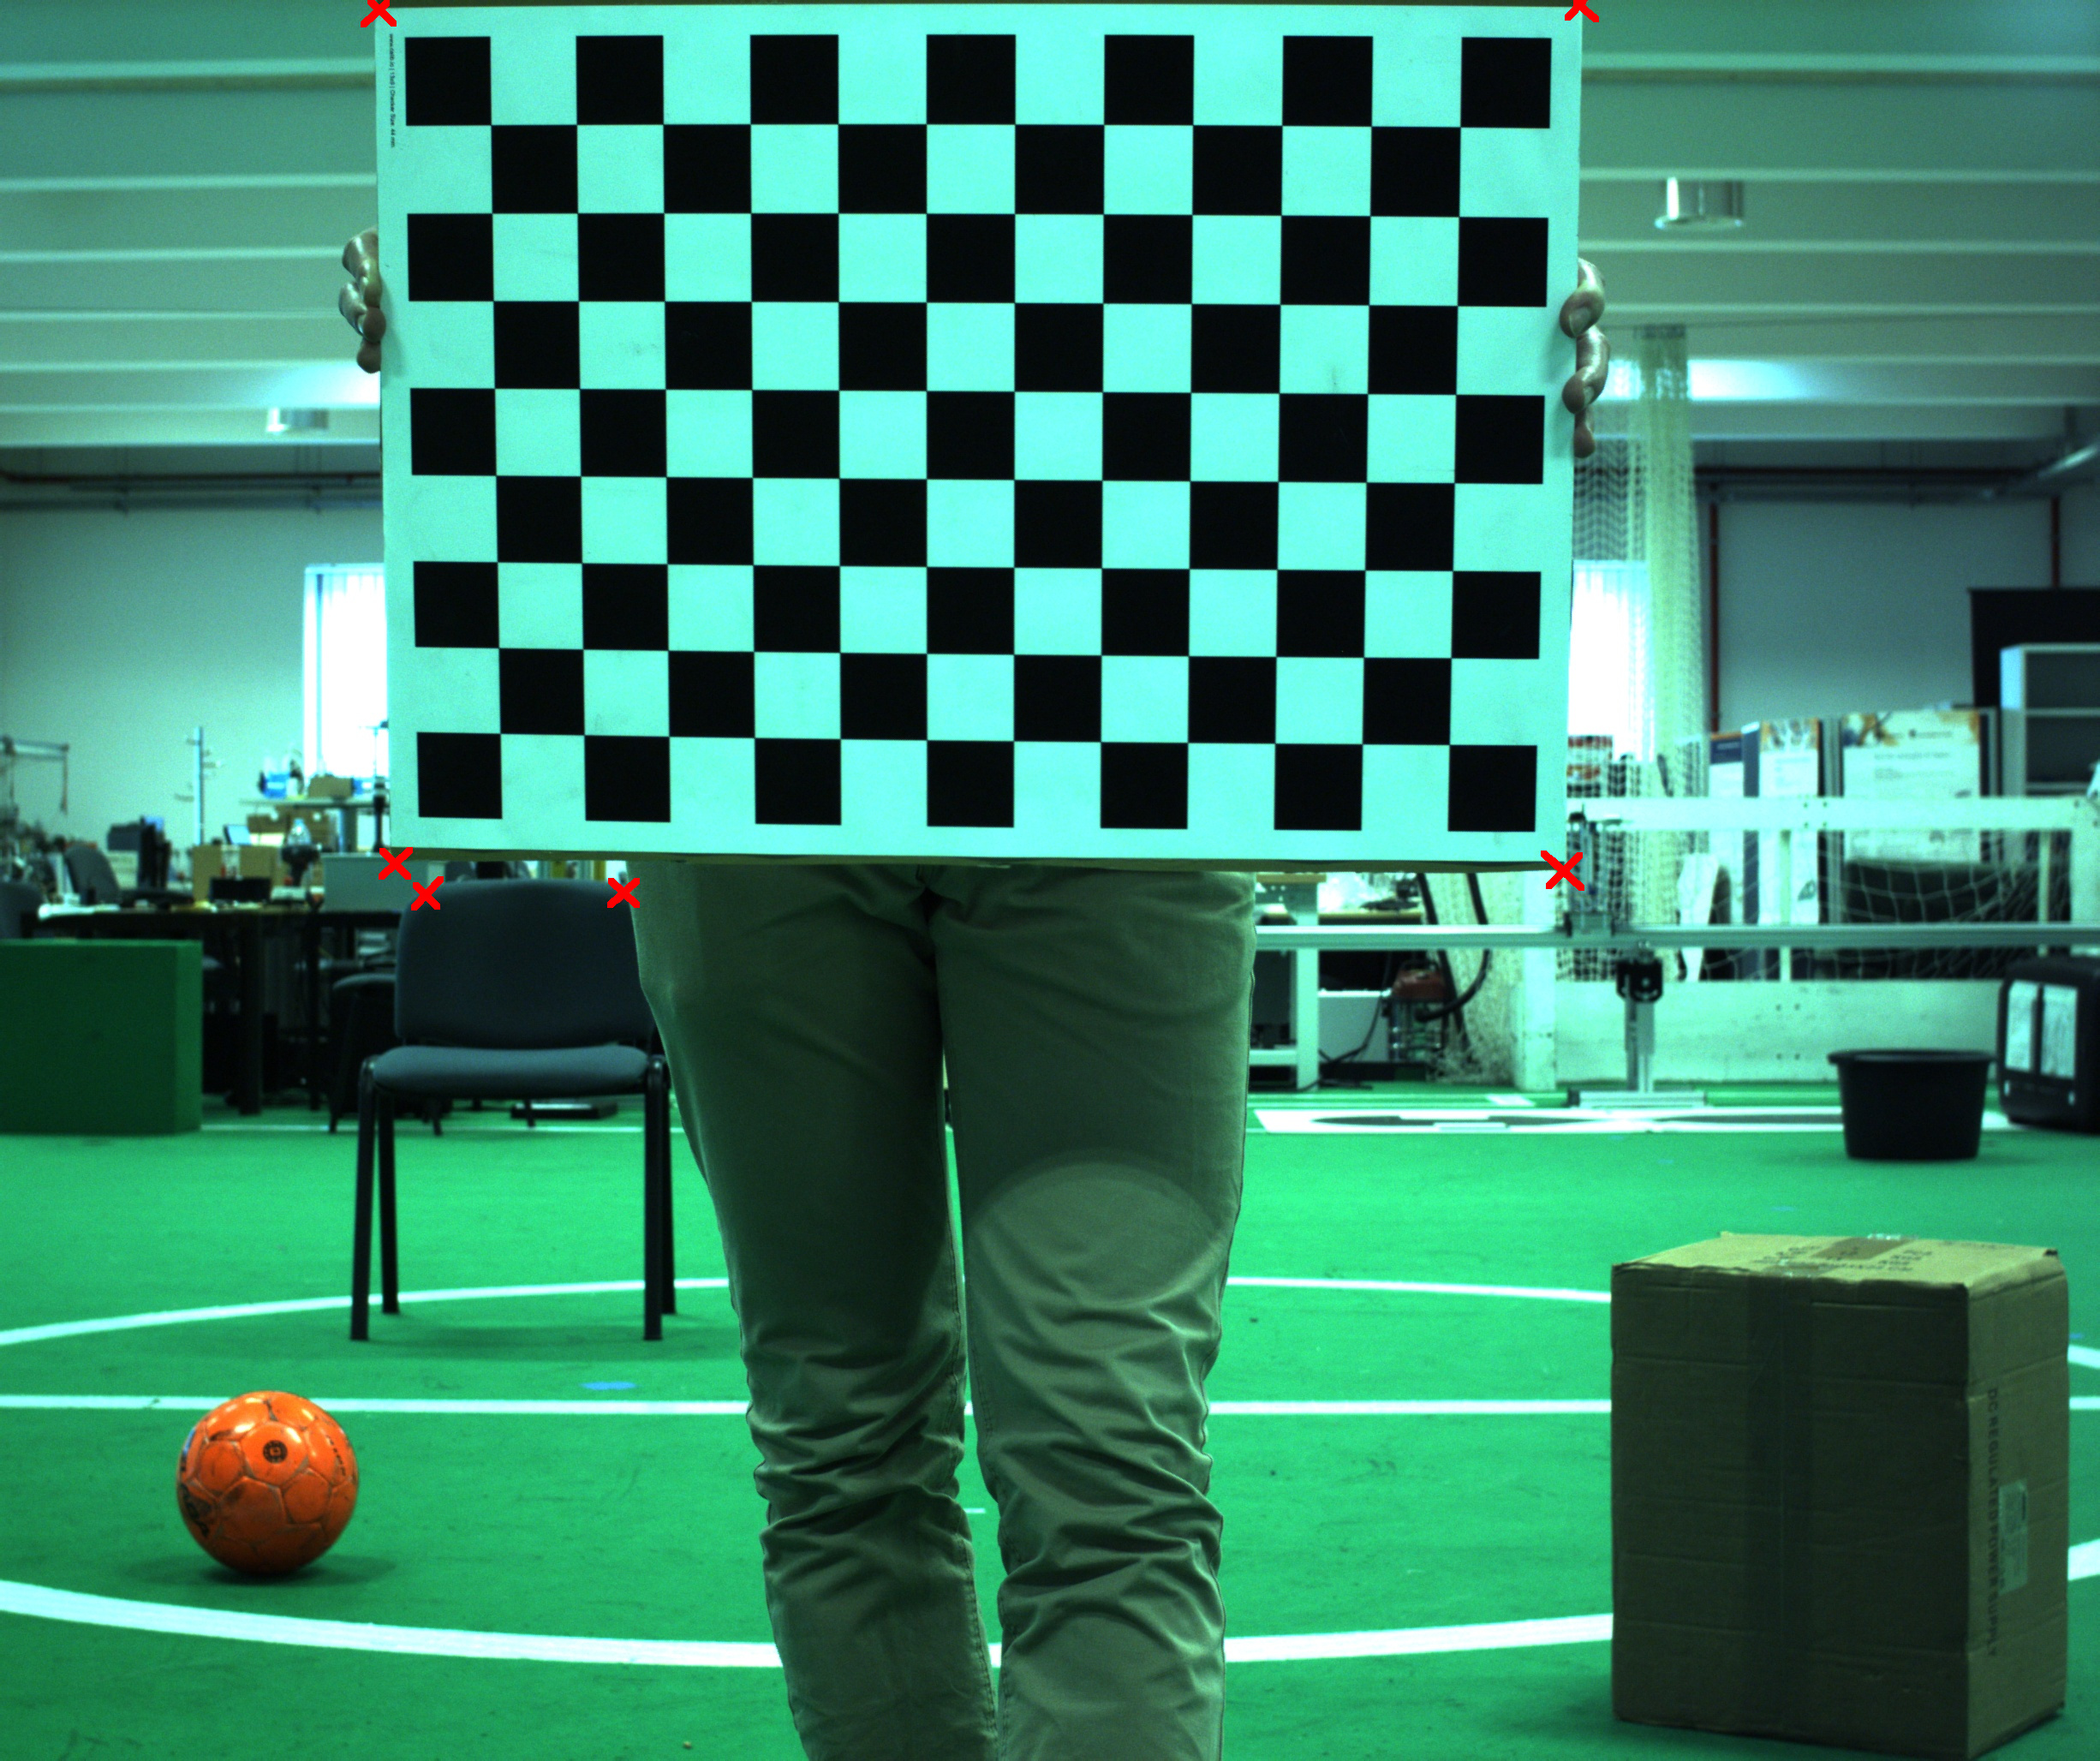
\includegraphics[width=\textwidth]{img/calibration/camera-extrinsic-calibration-points-draw.jpg}
		\caption{}
		\label{fig:extrinsic-calibration-correspondences:camera}
	\end{subfigure}
	\qquad
	\begin{subfigure}[c]{0.55\textwidth}
		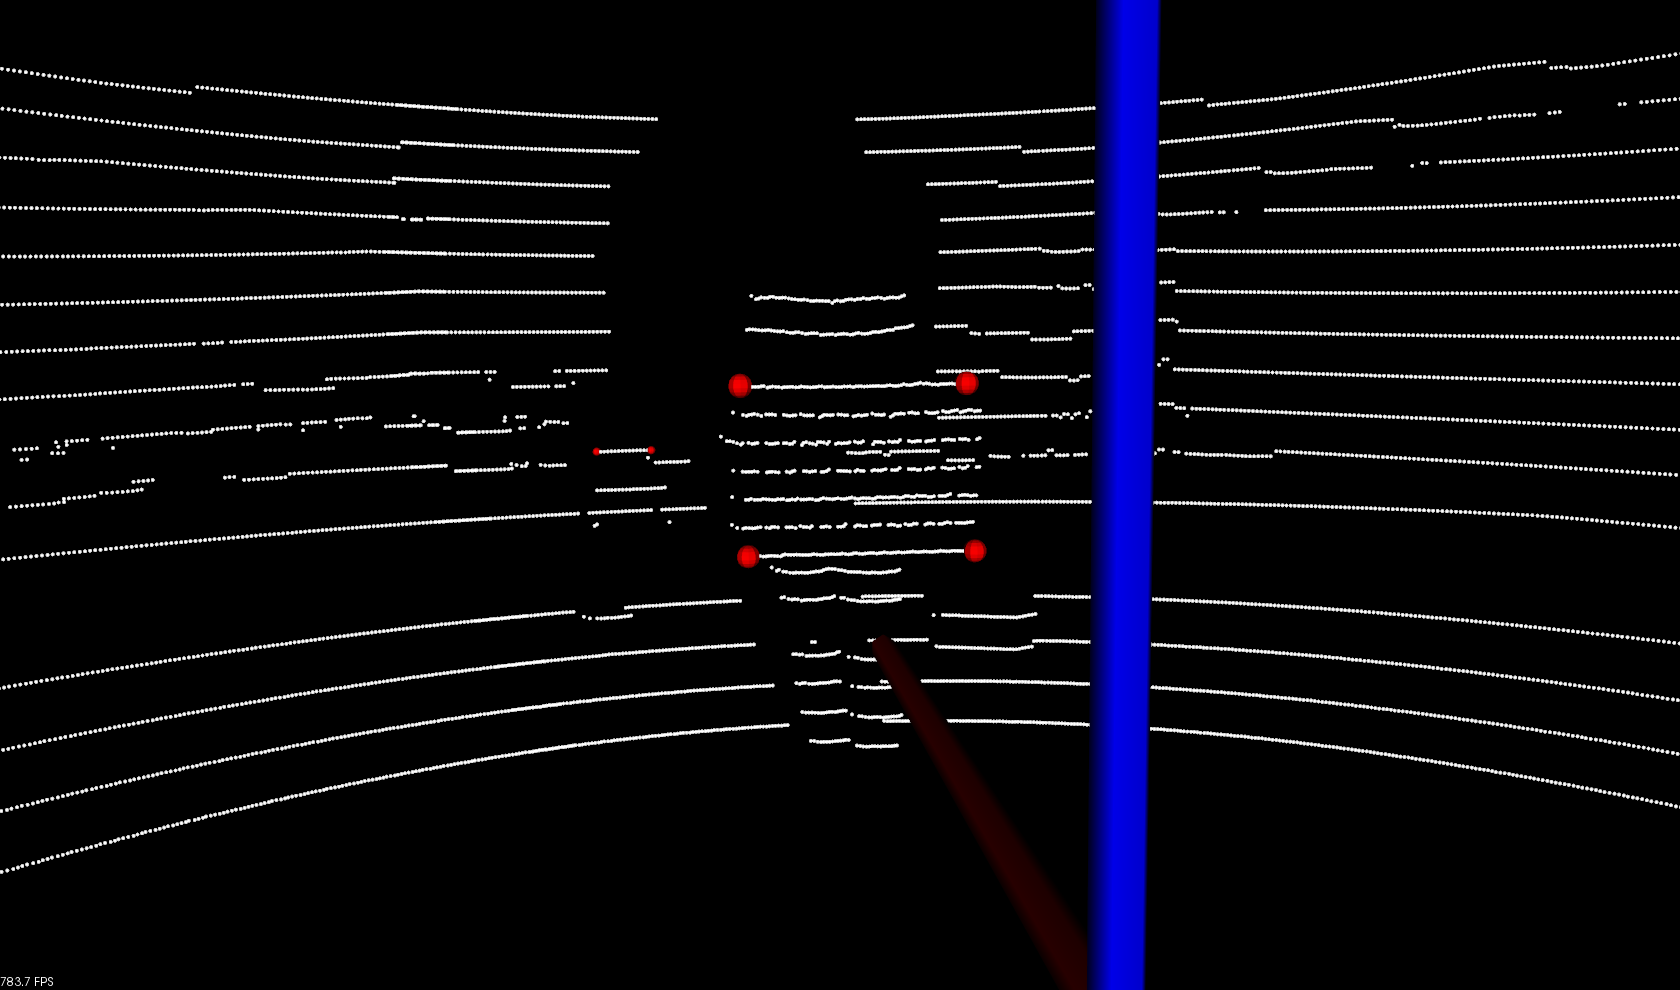
\includegraphics[width=\textwidth]{img/calibration/lidar-extrinsic-calibration-points.png}
		\caption{}
		\label{fig:extrinsic-calibration-correspondences:lidar}
	\end{subfigure}
	\caption[Correspondences selected on the image and point cloud for extrinsic calibration between the two.]{Image~(\subref{fig:extrinsic-calibration-correspondences:camera}) and Region of the Point Cloud~(\subref{fig:extrinsic-calibration-correspondences:lidar}) used on the extrinsically calibration between the camera and the \ac{lidar}. The correspondences are marked with red crosses or spheres, respectively, and correspond to the 4 corners of the chessboard and the limit of the chair on the background.}
	\label{fig:calibration-correspondences}
\end{figure}

After the manual selection of the points, the rotation and translation are obtained from the camera frame to the \ac{lidar} frame. If the transformation from the \ac{lidar} to the camera frame is required, the inverse transformation can be obtained by inverting the scalar component of the quaternion, $w$, as depicted in Equation~\eqref{eq:quaternion-inversion}. 

\begin{equation}
	\label{eq:quaternion-inversion}
	w^\text{LiDAR}_\text{camera} = - w^\text{camera}_\text{LiDAR}
\end{equation}

Extrinsic camera and \ac{lidar} calibration was performed whenever experimental measures were taken. The calibration for the camera intrinsic parameters given on Equation~\eqref{eq:camera-calibration-results} and the correspondences shown on Figure~\ref{fig:calibration-correspondences} are presented on below. On Figure~\ref{fig:extrinsic-calibration-frames}, a visualization of the experimental setup sensors coordinate frames and the transformation between them is given.

\begin{subequations}
	\label{eq:camera-to-lidar-transform}
	\begin{align}
		t = \begin{bmatrix}
			-0.156714088124  \\
			-0.0206731034739 \\
			-0.258170823407
		\end{bmatrix} \nonumber
		& \qquad
		q = \begin{bmatrix} 
		 0.4872192 \\
		-0.4999094 \\
		 0.5216904 \\
		-0.4904560
	\end{bmatrix} \nonumber
	\end{align}
\end{subequations}

\begin{figure}[H]
	\centering
	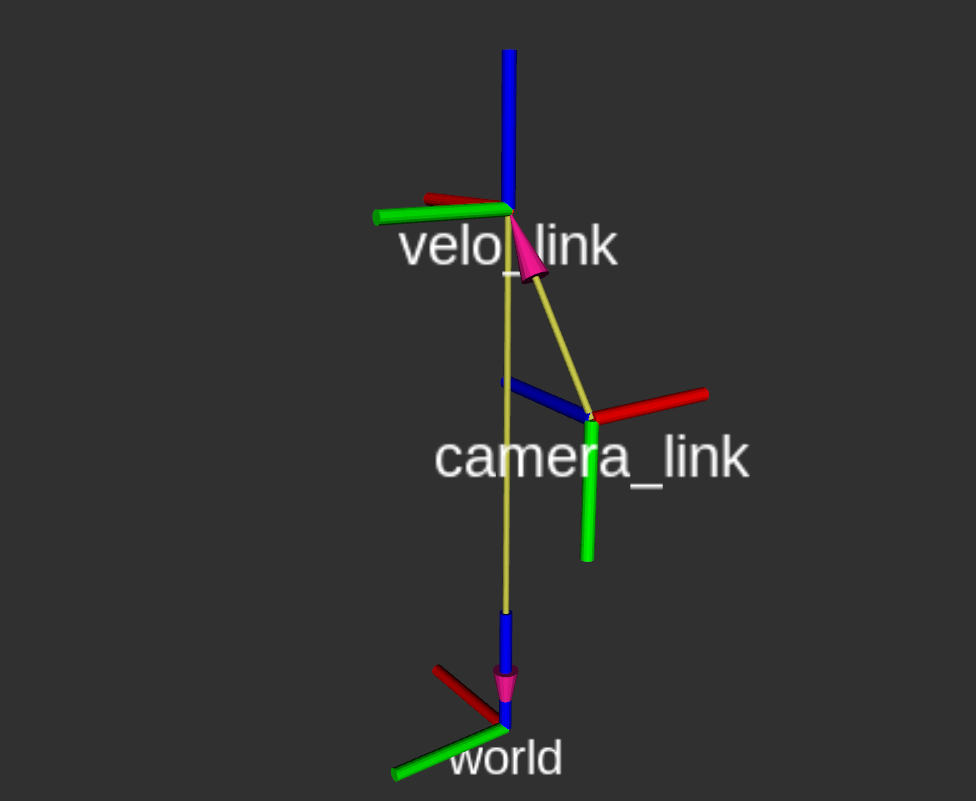
\includegraphics[width=0.5\textwidth]{img/calibration/extrinsic-calibration-frames.png}
	\caption[Experimental setup TF tree coordinate frames.]{TF visualization on \texttt{Rviz} of the TF tree between the experimental setup coordinate frames. \texttt{velo\_link} and \texttt{camera\_link} represent the coordinate frames of the Velodyne VLP-16 \ac{lidar} and the Manta \ac{avt} G-504C, respectively. The \texttt{world} coordinate frame represents the positioning of the \ac{lidar} in the world, which in this case is an offset to the vertical positioning of the \ac{lidar}.}
	\label{fig:extrinsic-calibration-frames}
\end{figure}

\subsection{Comparison with \ac{kitti}}
\label{subsec:calibration:kitti-comparison}

On \ac{kitti}, the number of coordinate frames is greater and have more complex interactions. While on the experimental setup the coordinates frames are all fixed, on \ac{kitti}, there is only one fixed frame, \texttt{world}. The car coordinate frame is named \texttt{base\_link} and the transformation between the \texttt{base\_link} and the camera are time-dependent.

On the car, every sensor has a coordinate frame, that is referred to the \texttt{base\_link} referential. From all the coordinate frames, that can be seen on~\cite{Geiger2013a}, the required during this research are:

\begin{itemize}
	\item \texttt{velo\_link}: Velodyne HDL-64E \ac{lidar} coordinate frame;
	\item \texttt{camera\_color\_left}: coordinate frame of the RGB camera selected for this research;
	\item \texttt{imu\_link}: \ac{imu} coordinate frame;
	\item \texttt{base\_link}: car coordinate frame.
\end{itemize}

Comparing with our experimental setup, the \ac{lidar} coordinate frame is equal in name and the coordinate axis orientation. The camera frame only differs in their name (the coordinate axis orientation is similar). Our experimental setup do not contain an \ac{imu}, therefore there is no need for a \texttt{imu\_link}. 

Due to the experimental setup being static, the \ac{lidar} and its \texttt{velo\_link} coordinate frame is referred directly to the \texttt{world} frame with a static transforms. Since the setup does not move, there is no need for a \texttt{base\_link} frame, since it will always coincide with the world frame, because the scene is static. On Figure~\ref{fig:kitti-tf-frames}, a subset of \ac{kitti}'s coordinate frames is presented. The \texttt{world} coordinate frame is not visible on the figure. 

\begin{figure}[!ht]
	\centering
	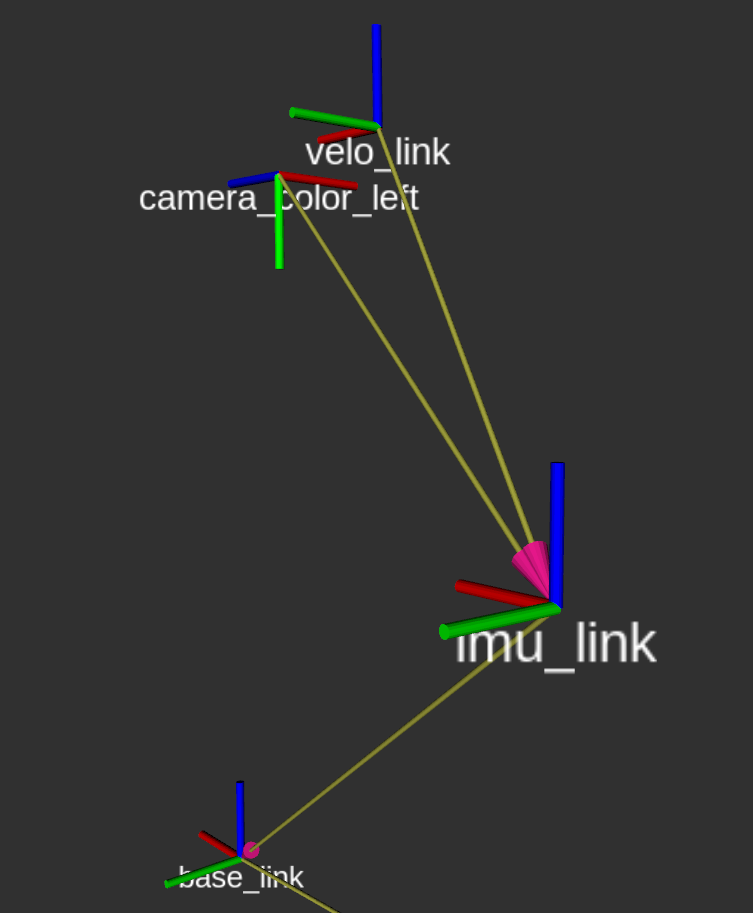
\includegraphics[width=0.5\textwidth]{img/KITTI/tf.png}
	\caption[Relevant \acs{kitti} TF tree coordinate frames.]{TF visualization on \texttt{Rviz} of the TF tree between a subset of \ac{kitti}'s setup coordinate frames. \texttt{velo\_link} and \texttt{camera\_color\_left} represent the coordinate frames of the Velodyne HDL-64E \ac{lidar} and the RGB left camera, respectively.}
	\label{fig:kitti-tf-frames}
\end{figure}

\section{Final Remarks}
\label{sec:calibration:final-remarks}

On this chapter, the experimental setup is presented and the intrinsic and extrinsic calibration of its sensors is detailed. Camera, \ac{lidar} and lens specifications are given and briefly discussed, along with their relative positioning, network setup and connection with the computer. Since camera will be used to understand and possibly mitigate \ac{lidar} interference through sensor fusion, we confirm that the camera is free from interference by the \ac{lidar} in a test without any other light sources.

Sensory calibration is performed to allow data acquisition from the camera and \ac{lidar} to construct the experimental setup dataset. Intrinsic camera calibration is carried by using \ac{ros} \texttt{camera\_calibrator.py} package and moving a chessboard in front of the camera, combining rotation and translation motions. Using Effective \acl{pnp}, the camera intrinsic matrix and the distortion coefficients for the lens are determined, which are used to rectify the camera image. Regarding \ac{lidar} calibration, the device comes calibrated by the manufacturer and only azimuthal and polar angle coefficients need to be loaded by the firmware and driver for measurement correction.

Extrinsic calibration between the camera and \ac{lidar} is performed to the determinate the rigid body transformation between the two, allowing the conversion of data between their coordinate frames. Our proposed algorithm is based on the selection of at least four $2D \leftrightarrow 3D$ correspondences between the image and the point cloud. A calibration pattern is not required. We adapt the work of Scaramuzza\etal and Brabec's, which is used to calibrate a camera, to determine the rigid body transform between the \ac{lidar} and camera, by solving for the joint rotation and translation matrix. To do so, our implementation consists of an image and point cloud visualizers, a node to receive the selected points and compute the rigid body transform and a client node to trigger the computation and saving of results.

From this chapter, our main takeout is a generic extrinsic calibration algorithm and its implementation on \ac{ros}, that can calibrated any \ac{ros} compatible monocular camera and 3D \ac{lidar}. We also intrinsically calibrate the camera, performing the first step of any computer vision project and obtain the rigid body transform between the sensors of our setup, to be used later. The work developed on this chapter is essential for the data fusion between the camera and \ac{lidar} (Chapter~\ref{chapter:sensor-fusion}) and object detection on image and estimating the correspondent bounding boxes on the point cloud (Chapter~\ref{chapter:object-detection}).

\chapter{\acs{lidar} and Camera Data Fusion}
\label{chapter:sensor-fusion}

Data fusion consists of combining the information from two or more sources of data, that can be of equal or different types, adding value to the data set and allowing newer insights that are not possible from the parts alone, such as a representation on which is possible to understand the depth differences  between objects that are colored for easier identification. Data fusion (and sensor fusion) are two widely topics used on several areas, such as Industry 4.0, robotics and autonomous vehicles; but on the context of this research, it means that the depth information from the \ac{lidar} is combined with the color data from the camera.

A pre-requisite to combine multiple sources of data is that the rigid body transformation between the sensors is known, which allows the conversion between \ac{lidar} and camera coordinate frames. Such rigid body transform is already obtained in the previous chapter, in Section~\ref{sec:calibration:extrinsic}. Examples of sensor fusion are also been presented in Figure~\ref{fig:point_cloud_camera_fusion_example} from Section~\ref{sec:sota:sensor-fusion}.

As detailed in Section~\ref{sec:sota:sensor-fusion}, two ways are possible for combining \ac{lidar} and camera data: presenting depth information overlaid on an image or color information on a point cloud. For the purpose of this work, we are only interested on the latter, as it provides, on our opinion, a better way to verify the correctness of the calibration of Chapter~\ref{chapter:calibration} and a more interesting \ac{lidar} interference analysis and possible mitigation.

\section{Combining \acs{lidar} and Camera Data}
``Point Cloud Coloring'' consists of augmenting the information contained on a point cloud by adding to each point a RGB triplet indicating the point's color. Velodyne point clouds, besides the Euclidean coordinates of the point, also contain the intensity measurement and the laser ID/ring number\footnote{Laser ID and ring number are two concepts that can be inter-changed without loss of context. The former is more commonly used on written text while the latter is used on the source code.} of the laser and photodetector pair.

To add color data to the point cloud, two approaches can be used, depending on the source and target coordinate system:

\begin{enumerate} 
	\item \textbf{Camera $\rightarrow$ \ac{lidar}:} the camera is the source coordinate system and \ac{lidar} is the target coordinate system. The camera data is converted from the 2D image  matrix index to the \ac{lidar} 3D coordinate frame;
	\item \textbf{\ac{lidar} $\rightarrow$ Camera:} the \ac{lidar} is the source coordinate system and the camera is the target coordinate system. \ac{lidar} data is converted from the 3D \ac{lidar} coordinate frame to the camera's.
\end{enumerate}

Both approaches have their advantages and drawbacks, which will be discussed on the next two sub-sections.

\subsection{Camera $\rightarrow$ \acs{lidar}} 
Using the camera as the source coordinate system implies that the 2D pixel's information must be converted to a tridimensional format. However, when applying Equation~\eqref{eq:camera_transform_full}, depth and scale information are lost, and without further constraints, it is not possible to determine the position of the 3D point that gave origin to the image pixel\footnote{For more information, the reader is advised to research on Single View Geometry or see Part I of~\cite{mvg_book}.}. 

Therefore, re-projecting pixels to a 3D coordinate system is an under-determined system of equations, causing the geometric representation of the system to be either a ray or a quadrangular pyramid, depending on the camera sensor being considered continuous or discrete, respectively. For simplification, from now on it is considered that the 3D representation of a pixel is a ray that contains the focal point and the pixel to be projected.

After computing the ray coefficients, for data fusion the pixels projected into rays must be matched to the point cloud points. Due to the sparse nature of the \ac{lidar} data, most of the pixels do not have a correspondence with 3D points, and a criterion to reduce the number of pixels projected could be used. For the Velodyne VLP-16, the azimuthal step is \SI{0.2}{\degree} and the polar step \SI{2}{\degree}. Therefore, the number of pixels to be projected can be reduced, but that reduction must be accompanied by a solution for dealing with multiple matches and point color from multiple pixels. Dealing with multiple matches implies proposing an algorithm that decides  how to color a group of 3D points that are the correspondence of a group of pixels, since a group of pixels contains pixels with different RGB values.

Once the pixels have been projected to rays on the camera coordinate frame, before they can be matched with the \ac{lidar} points, the coefficients that define the ray must be converted to the \ac{lidar} coordinate frame.

The major drawback of this method is that for high definition images, the considerations on reducing the number of projected pixels must be taken, since the number of rays to be computed can become impractical. For our experimental setup, not considering any optimizations, would require the computation of more than 5 million rays, their projection to the point cloud coordinate frame and matching with the point cloud points.


\subsection{\acs{lidar} $\rightarrow$ Camera}
\label{subsec:sensor-fusion-lidar-to-camera}
Projecting \ac{lidar} data to the image can be performed by re-purposing Equation~\eqref{eq:camera_transform_full}: the object points are considered to be \ac{lidar} 3D point coordinates and the joint rotation and translation matrix are replaced by the rigid body transformation between the \ac{lidar} and the camera coordinate frame, which can be obtained by inverting the rigid body transformation determined in Section~\ref{sec:calibration:extrinsic}. As detailed in sub-Section~\ref{subsec:calibration:extrinsic-results}, this inversion, since we are using a quaternion notation, is equivalent to change the quaternion scalar component to its symmetric number, as depicted in Equation~\eqref{eq:quaternion-inversion}.

Projecting \ac{lidar} data to the camera coordinate frame results on a 2D point that can be used to index the image pixel matrix. However, since the \ac{lidar} \ac{fov} is wider than the camera's, it is necessary to verify if the representation of the \ac{lidar} point on the camera referential corresponds to a valid image pixel. The camera orientation should also be considered, since the \ac{lidar} points on its negative z-axis mirror the points of it positive z-axis, corresponding to the same pixel.

To translate and rotate the \ac{lidar} data to match the camera coordinate frame, the \ac{lidar} points are projected to the image using the affine\footnote{Affine coordinates are the coordinates of a Projective space, such as the Cartesian coordinates are the coordinates of a Euclidean space.} transformation of Equation~\eqref{eq:lidar-to-camera-affine}. 

\begin{equation}
	\label{eq:lidar-to-camera-affine}
		\begin{bmatrix}
			U \\
			V \\
			W
		\end{bmatrix}
		= P \times
		\begin{bmatrix}
			X \\
			Y \\
			Z \\
			1
		\end{bmatrix}
\end{equation}

To obtain the normalized 2D Point that represents the coordinates of a pixel in the camera coordinate frame, Equation~\eqref{eq:camera-matrix-idx-normalized} is used.

\begin{equation}
	\renewcommand\arraystretch{1.5}
	\label{eq:camera-matrix-idx-normalized}
	\begin{bmatrix}
		u \\
		v
	\end{bmatrix}
	= 
	\begin{bmatrix}
		\frac{U}{W} \\
		\frac{V}{W}
	\end{bmatrix}
\end{equation}


\section{Implementation}
\label{sec:sensor-fusion:implementation}
The implementation we opt to follow is the second method described: \ac{lidar}  $\rightarrow$ Camera, for three reasons:

\begin{enumerate}
	\item The mathematical transformation is similar to the camera projective geometry and calibration procedure;
	\item The correspondences between the data are more easily established;
	\item The reduced number of correspondences that need to be computed.
\end{enumerate}


To fuse the \ac{lidar} and camera data, a ``Point Cloud Coloring'' \ac{ros} node is implemented. This node is responsible for synchronizing the camera information and images with the point cloud data from the \ac{lidar}, triggering a callback function on every synchronization event. On the callback, the point cloud points are translated and rotated to match the camera coordinate frame and the points are projected to the image using the affine transformation described previously in Equation~\eqref{eq:lidar-to-camera-affine}.

The full node graph is presented in Figure~\ref{fig:sensor-fusion-rosgraph}, in Appendix~\ref{appendix:appendix-diagrams}, containing not only the node responsible for the data fusion itself, but also the other nodes required for the calibration. In this image, \texttt{camera} nodes and topics are boxed together, visually separating the two types of sensors: camera and image; and \ac{lidar} and point clouds.

A \texttt{tf} (short for transform) block can also be shown, receiving the output of two nodes: \texttt{LiDAR\_to\_world} and \texttt{compute\_rigid\_body\_transform}. The first a static transform publisher, that sends the rotation quaternion and translation vector that can be used to positioning the \ac{lidar} in the referential for the test scenario; the second is a node that publishes the rigid body transform obtained in Section~\ref{sec:calibration:extrinsic}. Lastly, \texttt{Point\_Cloud\_Coloring} node receives all this data and publishes a colored point cloud, at $\approx \SI{4.2}{\hertz}$, more than two times slower that the \SI{10}{\hertz} at which ``common'' point cloud data is published on the \ac{ros} network. \texttt{Rviz} is a \ac{ros} multi-sensor data visualizer.


%\begin{figure}[!ht]
%	\centering
%	\def\svgwidth{\columnwidth}
%	\graphicspath{{img/sensor_fusion/}}
%		\includesvg{img/sensor_fusion/sensor-fusion-with-calibration-print}
%		\caption[\ac{ros} node graph implemented for coloring the point cloud.]{\ac{ros} graph with the nodes used in data fusion between the \ac{lidar} and camera. The camera and \ac{lidar} topics are separated visually, with the camera still requiring the \texttt{image\_proc} package to de-Bayering the raw image data. Data is fused on the node \texttt{Point\_Cloud\_Coloring}, using the RGB image, point cloud, camera parameters and rigid body transforms.}
%	\label{fig:sensor-fusion-rosgraph}
%\end{figure}


\section{Results}
The algorithm described on the section above is applied both to our experimental dataset and \ac{kitti}'s, being the results compared. Two test locations are used: a larger and a smaller room, with the user and the objects of interest at different distances from the camera.

Fusing the data on our experimental dataset (sub-Section~\ref{subsec:sensor-fusion:experimental-dataset}), requires applying the calibration steps detailed in Chapter~\ref{chapter:calibration}:

\begin{enumerate}
	\item Intrinsic camera calibration (Section~\ref{sec:calibration:camera}) to determine the camera intrinsic parameters and its projection matrix, to rectify the image and project world points to the camera coordinate frame;
	\item \ac{lidar} offset calibration, by loading the azimuthal and polar correction parameters that intrinsically calibrate the \ac{lidar};
	\item Rigid body transformation determination, by selecting the correspondences that allow the extrinsic calibration between the \ac{lidar} and camera.
\end{enumerate}

After these steps, our experimental data can be fused using the implementation described in Section~\ref{sec:sensor-fusion:implementation}.

Regarding \ac{kitti}'s dataset, the steps mentioned above do not have to be taken and sensor-fusion can be done directly using the dataset data, since the rigid body transformation between sensors is already available. Results for this dataset are shown in sub-Section~\ref{subsec:sensor-fusion:kitti}.

\subsection{Experimental Dataset}
\label{subsec:sensor-fusion:experimental-dataset}
The results using the experimental data shown in calibration are presented, in Figure~\ref{fig:cambada-sensor-fusion}. Due to the nature of the figure (an image of a tridimensional colored point cloud), one does not instantly recognize the chessboard pattern, the ball and the person; and might even consider the results as unsatisfactory. 

\begin{figure}[!ht]
	\centering
	\begin{subfigure}[t]{0.45\textwidth}
		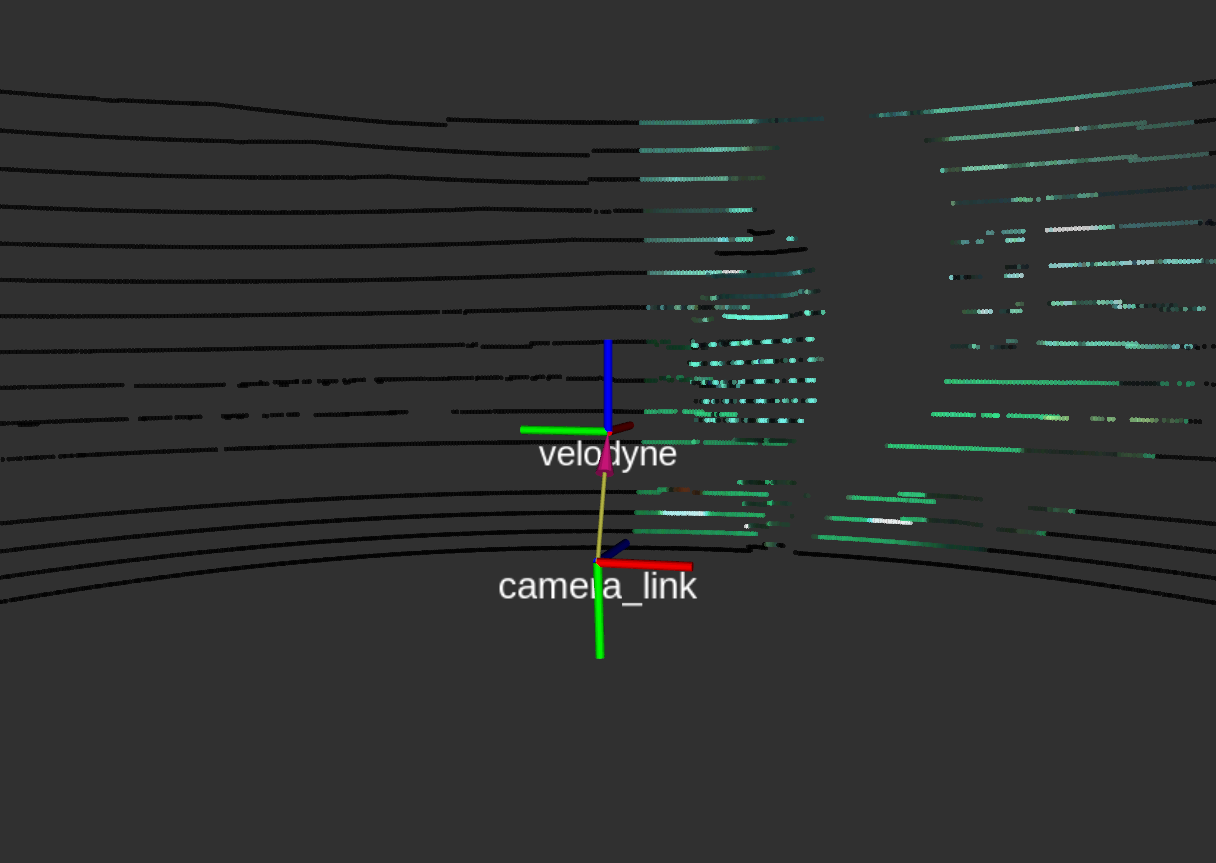
\includegraphics[width=\textwidth]{img/sensor_fusion/cambada_fusion_points.png}
		\caption{}
		\label{fig:sensor-fusion:cambada-points}
	\end{subfigure}
	\qquad
	\begin{subfigure}[t]{0.45\textwidth}
		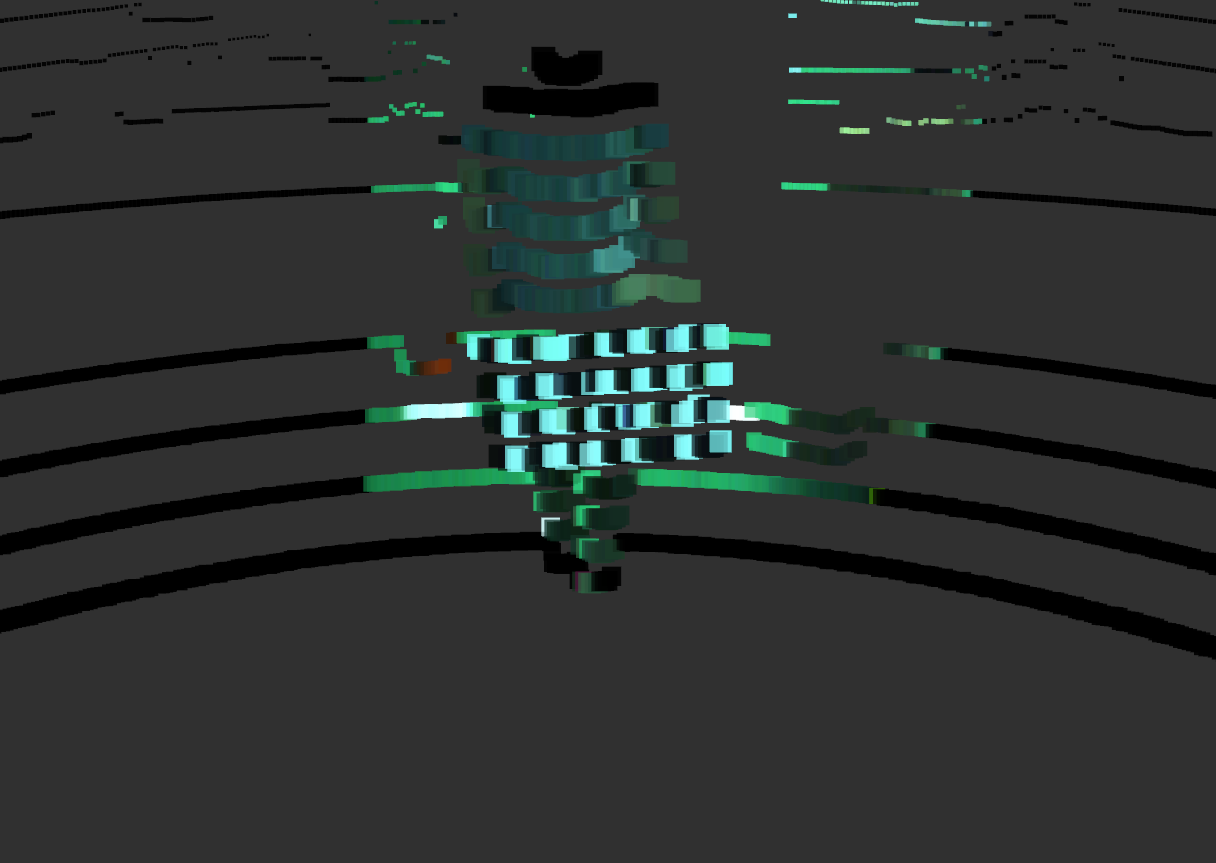
\includegraphics[width=\textwidth]{img/sensor_fusion/cambada_fusion_squares.png}
	\caption{}%The rectangles presented on the image have a size 4 cm and a transparency of 70\%.}
		\label{fig:sensor-fusion:cambada-squares}
	\end{subfigure}
	\caption[Colored point clouds computed for the datasets on \acs{irislab}.]{Data fusion between the camera and the \ac{lidar} on a \ac{msl} field. The colored point cloud is presented on sub-figure: (\subref{fig:sensor-fusion:cambada-points}) with points of 4 pixels and 70\% of transparency, with the coordinate frames also shown; (\subref{fig:sensor-fusion:cambada-squares}) with squares of \SI{4}{\centi\meter} of size and a transparency of 70\%.}
	\label{fig:cambada-sensor-fusion}
\end{figure}

However, such results are obtained with a low point density (VLP-16 only has 16 lines of data\footnote{Actually, our Velodyne VLP-16 has one of its lasers out of order, therefore we only have 15 lines of data.}) and a distance from the objects to the camera (a few meters). 

Another test, from the preliminary stages of the work, show the colored point cloud on \ac{it} 2 Dark Room, a smaller room where some tests were carried. On this case, the objects of interest are closer, so the colored point cloud has a better point cloud density, as shown in Figure~\ref{fig:dark-room-sensor-fusion}, 

\begin{figure}[!ht]
	\centering
	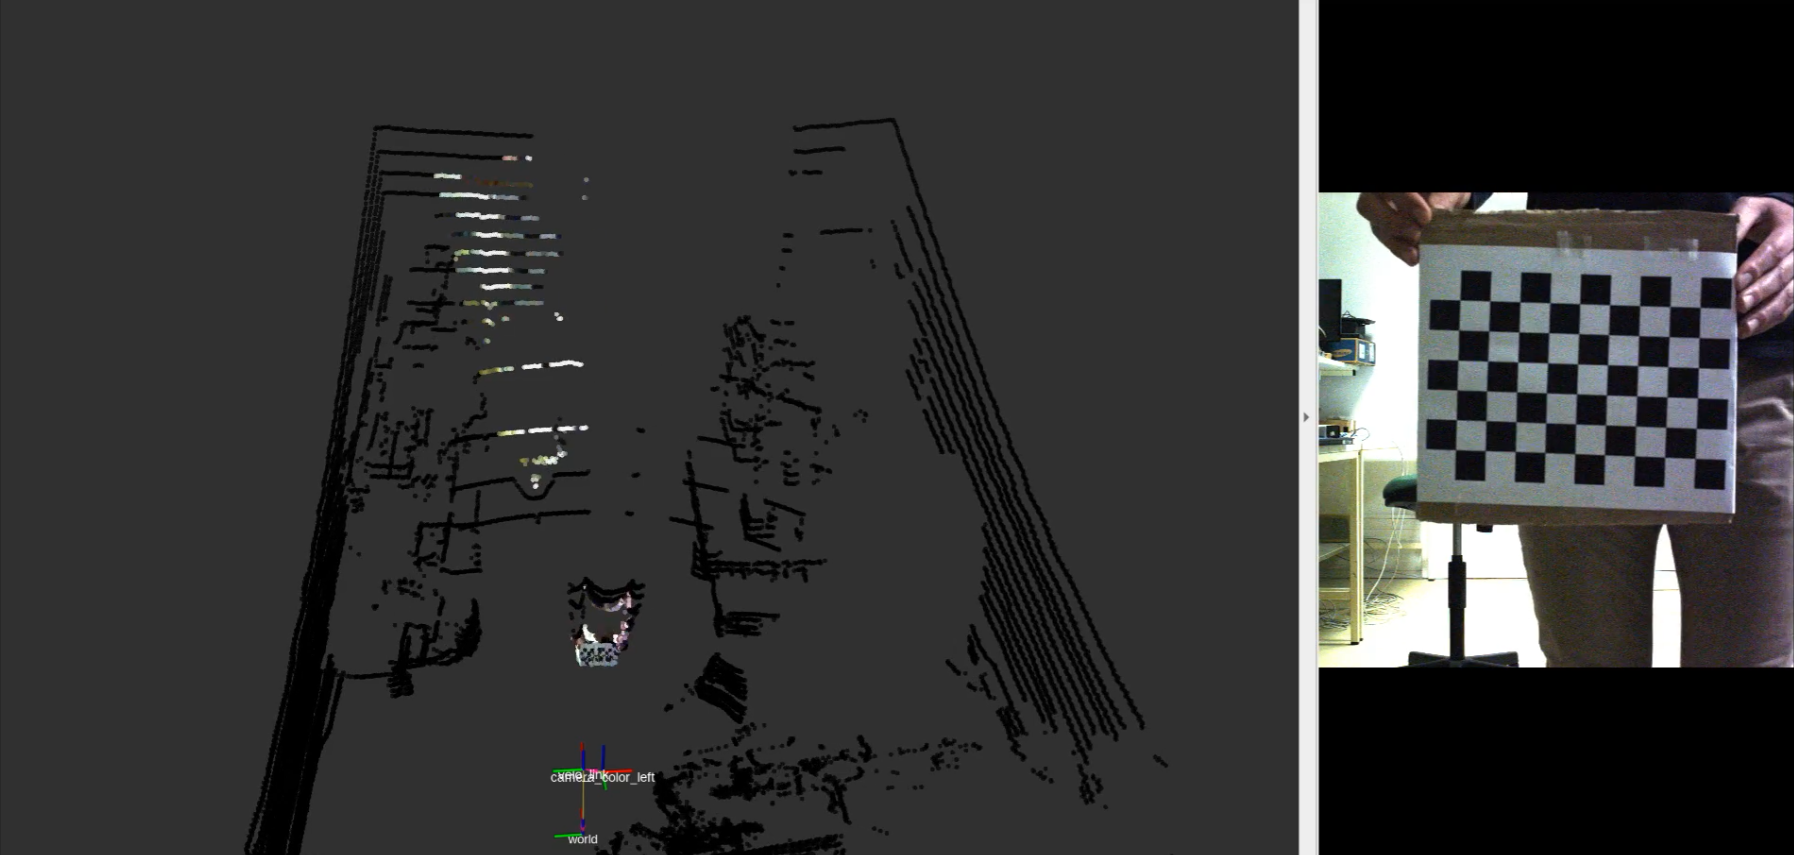
\includegraphics[width=0.7\textwidth]{img/sensor_fusion/dark-room-sensor-fusion.png}
\caption[Example of preliminar data fusion on \acs{it} 2 Dark Room.]{Data fusion between the \ac{lidar} and the camera data. On the left is the colored point cloud and on the right the image. The difference between this and the colored point clouds presented in Figure~\ref{fig:cambada-sensor-fusion} is that the objects of interest are closer to the camera and the experimental setup is placed inside a small room.}
	\label{fig:dark-room-sensor-fusion}
\end{figure}

\subsection{\acs{kitti} Dataset}
\label{subsec:sensor-fusion:kitti}
Applying the developed nodes to \ac{kitti} data set, which uses a Velodyne HDL-64E, with 64 pairs of laser beams and photodetectors, having 4 times more lines than our setup, results on the colored point cloud presented in Figure~\ref{fig:kitti-sensor-fusion}. This cloud has some differences when compared with the figures~\ref{fig:cambada-sensor-fusion} and~\ref{fig:dark-room-sensor-fusion}, such as:

\begin{itemize}
	\item The increase of photorealism in the colored point cloud, due to the increase in the number of laser beams;
	\item The dynamic scenario on \ac{kitti} dataset, compared to ours static experimental scenario.
\end{itemize}

In Figure~\ref{fig:kitti-sensor-fusion}, a mismatch between the top and bottom part of the sub-figures can be observed, even if accounting for the different \ac{fov} and view port for the camera and \ac{lidar}. This mismatch is due to the processing delay introduced by the point cloud coloring \ac{ros} node, which results on the colored point cloud being published to the \ac{ros} network with a large delay and our implementation cannot keep up with the publishing demand of \ac{kitti}'s dataset data rate, which causes the mismatch between the points positioning along the car direction of movement. Such mismatch and delay, however, is only due to the hardware  specifications running the algorithm, as is completely eliminated by using a computer with better specifications, specially on \ac{ram}, \ac{gpu} and \ac{cpu}.

\begin{figure}[!ht]
	\centering
	\begin{subfigure}[c]{0.8\textwidth}
		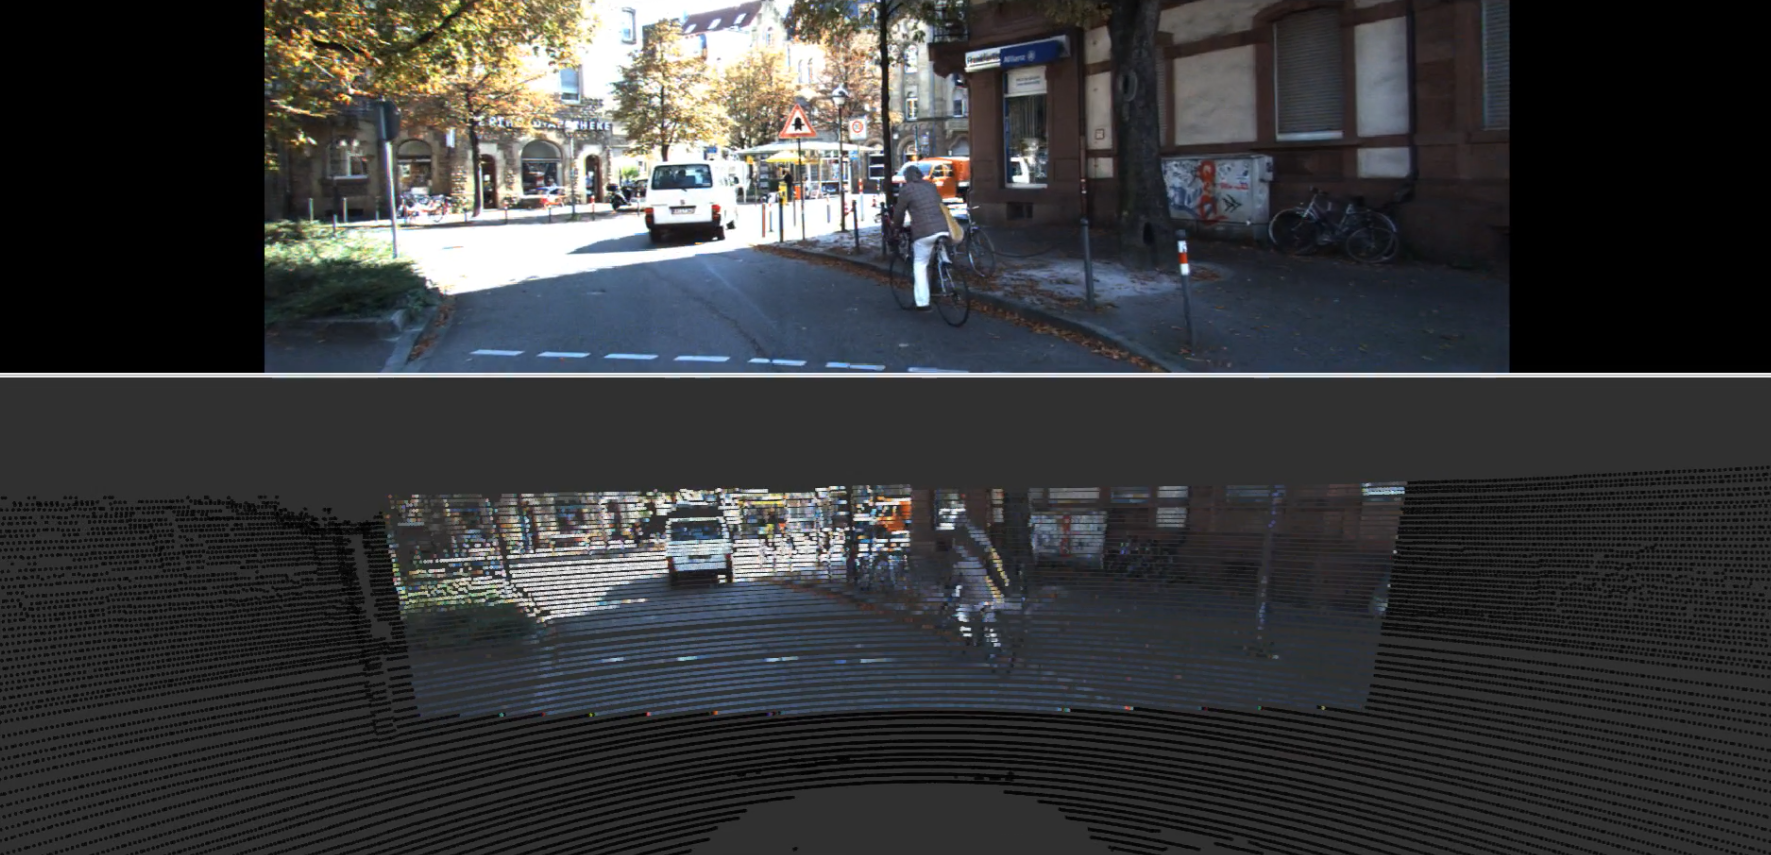
\includegraphics[width=\textwidth]{img/sensor_fusion/kitti-sensor-fusion-1.png}
		\caption{}
		\label{fig:kitti-sensor-fusion-1}
	\end{subfigure}
	\\ \vspace{4mm}
	\begin{subfigure}[c]{0.8\textwidth}
		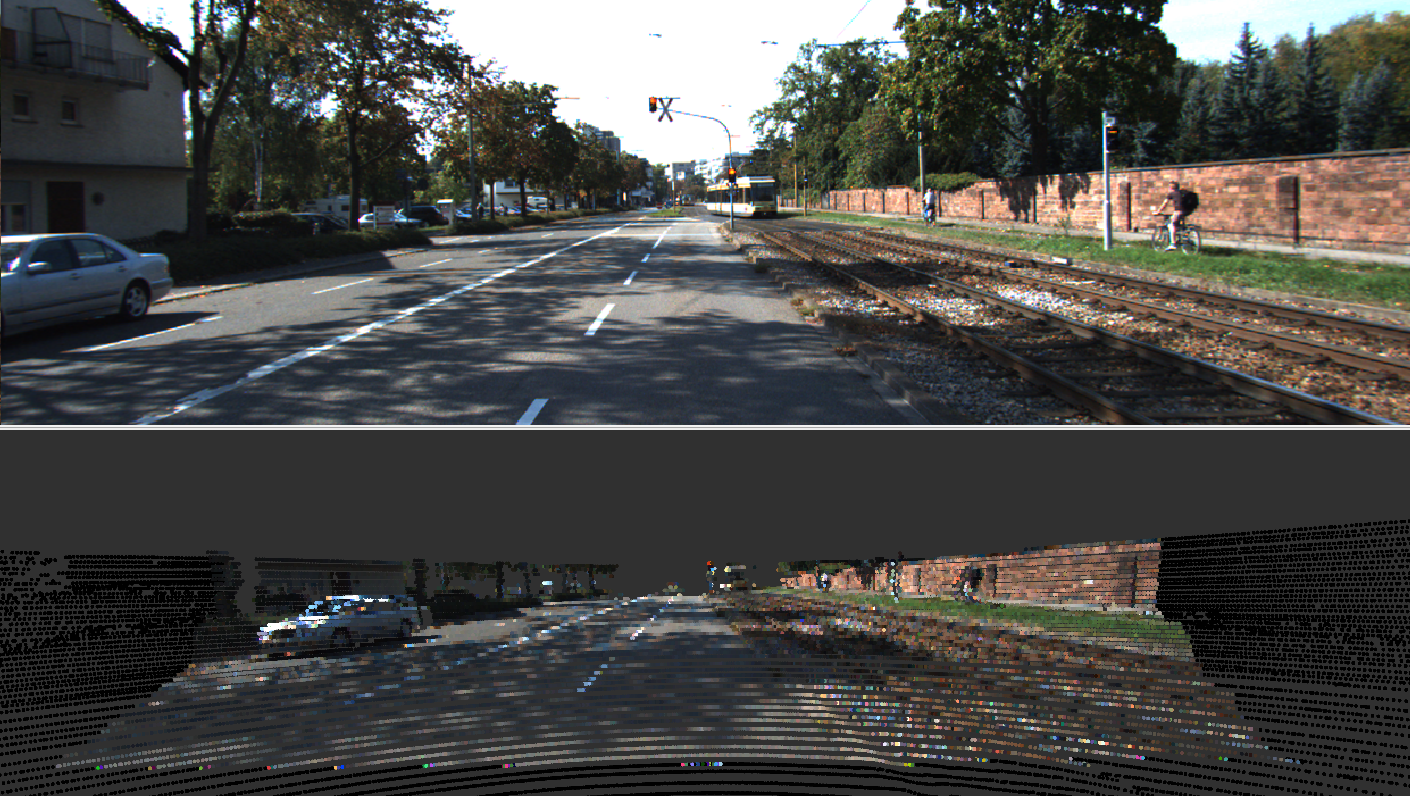
\includegraphics[width=\textwidth]{img/sensor_fusion/kitti-sensor-fusion-2.png}
		\caption{}
		\label{fig:kitti-sensor-fusion-2}
	\end{subfigure}
	\caption[Example of data fusion on \acs{kitti} dataset.]{Data fusion between camera and \ac{lidar} applied to the \ac{kitti} dataset. On the top there is the image and on the bottom the colored point cloud, displayed in points with 6 pixels of size and 50\% of transparency. Note that there is a mismatch between the image being shown and the image used to create the colored point cloud of 2 frames. In sub-Figure~(\subref{fig:kitti-sensor-fusion-1}), a cyclist and the car can clearly been identified on the colored point cloud and in sub-Figure~(\subref{fig:kitti-sensor-fusion-2}), the car, the wall, the road lines and the shadows can clearly be seen on the colored point cloud.}
	\label{fig:kitti-sensor-fusion}
\end{figure}


\subsection{Impact of Point Cloud Density}
In Figure~\ref{fig:dark-room-sensor-fusion}, it is evident that coloring a point cloud results on the loss of many high level features that are present on an image. On the resulting colored point cloud can be difficult to distinguish any objects with the original image and if the viewer does not know the scene being displayed.

Such loss of context and high level features is due to the scarce nature of a point cloud in relation to the camera. A 16-beam \ac{lidar} would only have 16 rows of depth data, while a 5\ac{mp} image will have 1920 rows of pixels. That relation means that only 0.83\% of the image rows will have correspondences on the point cloud. Such is the case of our experimental data.

If the number of pixels is considered instead, assuming a high camera \ac{fov} of \SI{90}{\degree} (which is not our case, since monocular camera \ac{fov} is normally lower), a quarter of the point cloud points, $\approx 7200$ points are candidates for correspondences between camera and \ac{lidar}, resulting in only 0.14\% of pixels on the image having a correspondence to the point cloud. 

For \ac{kitti}'s dataset, a 2\ac{mp} camera is used and a 64 beams \ac{lidar}, which yields almost 6\% of the image rows having correspondences and $\approx 5.76\%$ of the image pixels having a corresponding point on the \ac{lidar} point cloud. Comparing with our setup, \ac{kitti} has a number of correspondences between image pixels and point cloud points 41 times higher, which results on the clear difference in photorealism between figures~\ref{fig:cambada-sensor-fusion} and~\ref{fig:dark-room-sensor-fusion} with Figure~\ref{fig:kitti-sensor-fusion}.

Therefore, we can conclude that merging color with the point cloud depth information, on the way we implemented it, is not a feasible solution either to generate better data for autonomous vehicles, assessing the calibration results or possibly mitigating the interference, due to the losses in the information contained on the image. A solution to tackle such sparsity of the \ac{lidar} data and its impacts on point cloud coloring would be to generate a mesh cloud  from a point cloud and then performing mesh cloud coloring and/or interpolation of the point cloud, in order to increase it point cloud density. Obviously, using a \ac{lidar} with a higher number of laser beams will help mitigate this problem.

\section{Final Remarks}
In this chapter, image and point cloud data are fused to create a ``colored point cloud'': a tridimensional point representation of the scene with depth and color information. The perks of such process are detailed in this chapter and a brief discussion of data fusion representation possibilities is provided: color on point cloud points or depth points overlapped on a 2D image. Our implementation chooses the former and two possible implementation are discussed.  

To implement such a data fusion, the rigid body transformation between the \ac{lidar} and camera must be determined, following the procedures in Section~\ref{sec:calibration:extrinsic} and the camera and \ac{lidar} must be intrinsically calibrated as indicated in Sections~\ref{sec:calibration:camera} and~\ref{sec:calibration:lidar}. Our implementation, a single online \ac{ros} node, assumes these steps are undertaken and listens to the \ac{lidar} and camera data, synchronizing it and coloring the point cloud. To determine the color of the points, we use the $2D \rightarrow 3D$ correspondences.

The results from this chapter show, visually, that the extrinsic calibration developed in Chapter~\ref{chapter:calibration} is correctly done. However, when comparing the results obtained on \ac{kitti} dataset with ours, our implementation lacks point cloud density to generate a photorealistic colored point cloud. Such drawback is caused by the low resolution of our \ac{lidar}\footnote{It should be noted that higher resolution \acp{lidar} for automotive were not available.}, and it reveals that this approach is not the correct one to create good models for autonomous driving. We would have hopped that by using a camera we could help mitigate this problem by merging data together, but this crude approach of projecting data from one coordinate frame to another is clearly not enough. We also briefly discuss the possibility to interpolate the data, to create a better model.


From this chapter, the main outcome is the understanding of transforming and fusing data from one to another, along with some insights on the possibility to use data/sensor fusion to mitigate the \ac{lidar} interference. Also, one takeout are the algorithms and libraries for point cloud to image re-projection, which are used to estimate the point cloud bounding box from the image bounding boxes, in Chapter~\ref{chapter:object-detection} since the mathematical description of the two problems is similar.

\chapter{Object Detection}
\label{chapter:object-detection}

Object Detection is a field of \acf{cv} whose objectives are to classify and locate objects in an image. Contrary to Object Recognition, whose sole goal is to identify which objects are present on a given image, object detection not only classifies the objects, but also outputs a bounding box and its position in the image. 

Using previous calibration and sensor fusion methods, detailed in Chapters~\ref{chapter:calibration} and~\ref{chapter:sensor-fusion}, respectively, this chapter builds on the previous work, allowing the segmentation of \acfp{roi} in the point cloud. Those \acp{roi} correspond to objects detected in the image, using image object detection methods on the camera feed but not on the \ac{lidar} data, since the obtained point cloud is expected to be interfered by other \acp{lidar}.

To successfully detect \acp{roi} in a given image and estimate the corresponding point-cloud section, three tasks are required: 
\begin{enumerate}
	\item Perform object detection on the camera image feed and compute the bounding boxes that delimit the \acp{roi};
	\item Select the objects' of interest bounding boxes from the pool of detected objects;
	\item Filter the point cloud on the \acp{roi} using the image bounding boxes information.
\end{enumerate}

\section{Object Detection on Image}
\label{sec:object-detection:image}

Object Detection in image state of the art nowadays is achieved with \acfp{cnn}, as detailed in Section~\ref{sec:sota:object-detection}, using deep learning techniques to train the \acl{nn}. From the available \acp{cnn} frameworks and \acl{sota} solutions, we choose the \acf{yolo} algorithm, due to its accuracy, real-time object detection capabilities and low resource usage\footnote{In this context, low resource usage is considered in comparison with other available solutions with similar detection accuracy. See a detailed comparison on~\cite{Redmon2018}.}~\cite{Redmon2016, Redmon2017}.

Pre-trained models are available for \ac{yolo}v2 and \ac{yolo}v3, using the \ac{pascal-voc} and \ac{coco}'s dataset. As detailed in Section~\ref{sec:sota:object-detection} and in~\cite{Redmon2018}, \ac{yolo}v3 surpasses its prior versions. Therefore, only the latter version will be used. 

For all 3 versions of \ac{yolo}, a lighter version is also available. The ``tiny'' \ac{yolo} versions, as referred by its author, consist of a smaller network that does faster classification at the expense of detection accuracy (bounding box position, dimensions and object class). On the context of this research, we are interested on having a precise estimation of the bounding boxes dimensions and position, since those will be used to detect the corresponding \acp{roi} on the point cloud. Therefore, \ac{yolo}'s v3 \ac{cnn} will be used, in detriment of its lighter version.

\subsection{Setup Specifications}
To summarize the decisions previously explained decisions, our image object detection methodology uses the \ac{yolo}v3 \ac{cnn}, with pre-trained weights for the \ac{coco} image dataset, running on the Redmon's \texttt{Darknet} framework wrapped in a multi-threaded \ac{ros} node. Darknet is compiled with \ac{cuda} and \ac{opencv} enabled, for \ac{gpu} acceleration and native visualization of the classified images with bounding boxes.

The image objection detection is done on a standard laptop with an Intel\cp~i7 \ac{cpu} and an Nvidia\cp~GeForce GT 740M. The relevant specifications are given on Table~\ref{tab:computer-specs}, along with information about the graphics card driver and \ac{cuda} version used.

\begin{table}[!ht]
	\renewcommand{\arraystretch}{1.2}
	\centering
	\begin{tabular}{@{}lp{7cm}l@{}}
		\toprule
		\multicolumn{2}{l}{Specification} & Value \\ \midrule
		\multicolumn{2}{l}{\emph{\ac{cpu}}} & \\
		\phantom{a} & Model   & Intel\cp~Core\texttrademark~i7-4700MQ \\
								& Maximum clock frequency & \SI{2.40}{\giga\hertz} \\
								& Number of cores & 4 \\ 
		\midrule
		\multicolumn{2}{l}{\emph{Graphic Card}} & \\
		\phantom{a} & Model   & Nvidia GeForce GT 740M \\
								& Maximum \ac{gpu} clock frequency & \SI{1058}{\mega\hertz} \\
								&	Maximum memory transfer rate & \SI{1840}{\mega\byte} \\
								&	Nvidia driver number & 418.87.01 \\
								& Total memory size & \SI{2048}{\mega\byte} \\
								& Bus width & \SI{64}{\bytes} \\
								& Theoretical Floating Point Operations & \SI{250.9}{\giga\flops} \\
		\midrule 
		\multicolumn{2}{l}{\emph{\ac{cuda}\texttrademark}} \\
								&	Version & 10.1 \\
								&	Dedicated memory size available on \ac{gpu}& \SI{2004}{\mega\byte} \\
								& Available \ac{cuda} cores on \ac{gpu} & 384 \\
		\bottomrule
	\end{tabular}
	\caption[Relevant specifications for \ac{cpu}, graphics card, \ac{cuda} and Nvidia\texttrademark driver.]{Relevant specifications for \ac{cpu}, graphics card, \ac{cuda} and Nvidia\texttrademark driver.}
	\label{tab:computer-specs}
\end{table}


\subsection{Integration with \ac{ros}}
\texttt{Darknet} (the \ac{nn} framework underlying \ac{yolo}) integrates with \ac{ros} using an Open-Source package developed by Marko Bjelonic~\cite{MarkoBjelonic}, \texttt{darknet-ros}. This package runs the Redmon's \texttt{Darknet} framework and wraps its configuration, input images and outputs results in a \ac{ros} node, containing an action server and several topics messages.

To configure the operation of \texttt{darknet-ros}, a \ac{ros} launch file is used. This launch file specifies the network model, configuration, weights and other \ac{ros} parameters, and is adapted from \texttt{darknet-ros} package launch file~\cite{MarkoBjelonic}. 

For image object detection, \texttt{darknet-ros} is used as a standalone node, with its input images being provided by a \texttt{rosbag} player, playing either the \ac{kitti} dataset data or the experimental setup. An \ac{opencv} image visualization window is embedded natively in \texttt{Darknet}, if it is compiled with \ac{opencv} enabled, and is used to view the classified images with bounding boxes.


\subsection{Results}
\label{subsec:object-detection:image-results}
It is out of the scope of this thesis to analyze or develop image object detection methods. Image object detection is used on this thesis as ``means to an end'': detecting \acp{roi} on image to compute their corresponding \acp{roi} on the point cloud. Therefore, exhaustive tests to compare the \ac{yolo} performance under different thresholds, lightning conditions and images were not carried. Instead, qualitative assessments were done to estimate a good threshold for confidence detection that maximise the number of detected objects.

\texttt{Darknet} is set with a default confidence threshold of 25\%~\cite{Redmon2016}. Nevertheless, from our findings, a threshold of 30\% improves the bounding box accuracy detection without drastically reducing the number of objects detected, being this the confidence threshold chosen for all tests.

With the relevant computer specifications presented in Table~\ref{tab:computer-specs}, the previous described method is able to classify images with 1.1 to 1.8 \ac{fps}, depending on the dataset used. Such reduced number of \ac{fps} is due to the image detection algorithms being running on a personal laptop without appropriated hardware for a real-time object detection. Then, to ensure that the classification process does not create a bottleneck on the system and messages are not dropped by \texttt{darknet-ros} node, since it cannot classify images as fast as they arrive, the \texttt{rosbag} player needs to be throttled, so that the publishing rate of messages can be slower.

Images are published at $\approx\SI{10}{\hertz}$ on the \ac{kitti} dataset and at \SIrange[range-units=single]{4}{8}{\hertz} on our experimental dataset. Therefore, if we throttle the \ac{ros} messages publishing rate to $10\%$ of the original rate, messages are published at a maximum of \SI{1}{\hertz} (slower than \texttt{Darknet-ros} image classification procedure), ensuring that no image frame dropping happens on the \texttt{darknet-ros} node. However, such throttling factor increases the duration of the file 10 times.

Exemplary results are presented in Figures~\ref{fig:kitti-object-detection} and~\ref{fig:experimental-object-detection}, both for the \ac{kitti} dataset and experimental data captured with the setup described in Section~\ref{sec:calibration:experimental-setup}.
	
\subsubsection{\ac{kitti} Dataset}
The previously described method is able to classify images at 1.3 to 1.8 \ac{fps}, on \ac{kitti} dataset. \ac{kitti} dataset majorly contains road scenarios, since the sensors are placed on a car and the setup is intended for self-driving vehicles (see Section~\ref{sec:sota:datasets}).

On Figure~\ref{fig:kitti-object-detection}, two exemplary results of the image detection algorithm used on the \ac{kitti} dataset are presented. On the top sub-figure,~\ref{fig:kitti-yolo-3}, a road intersection with several cars is presented. Despite the car's orientation, color and size, every car is detected correctly. In the middle of the sub-figure, three errors occur. One of the errors is related to a wrong car bounding box that contains two cars instead of a single car. This bounding box is near the second error, an undetected truck, occluded by a tree, in front of the factory, to the right side of the image. The third error is related to a tree top mistakenly labelled as a traffic sign, near the factory were the undetected truck is parked. The third refers to the undetected truck, which is partially occluded by a tree.

On the bottom sub-figure,~\ref{fig:kitti-yolo-2}, taken at the Karlsruhe Institute of Technology \textit{campus}, two errors are also present. In the center, a bounding box labelled as a person is actually a car and two road poles in a shadow area; and on the right, two persons are grouped together in one bounding box as if they were a single person.
	
\begin{figure}[ht!]
	\centering
	\begin{subfigure}[c]{0.8\textwidth}
		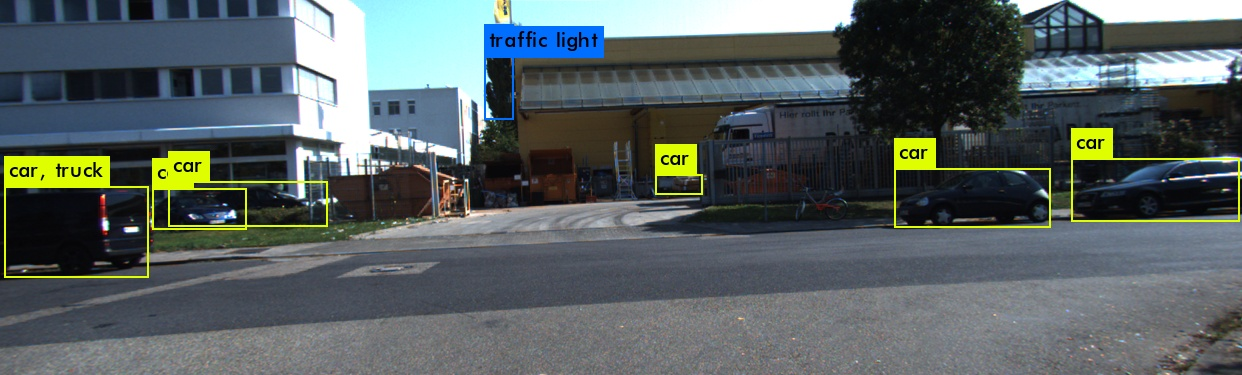
\includegraphics[width=\textwidth]{img/object-detection/kitti-4.jpg}
		\caption{Object detection on an urban area. Classification and bounding box dimensions and position are accurate, with exception to the traffic light bounding box, that is mistaken with a tree top, two cars in the middle of the image that are labelled as only one car and an undetected truck.}
		\label{fig:kitti-yolo-3}
	\end{subfigure}
	\\ \vspace{4mm}
	\begin{subfigure}[c]{0.8\textwidth}
		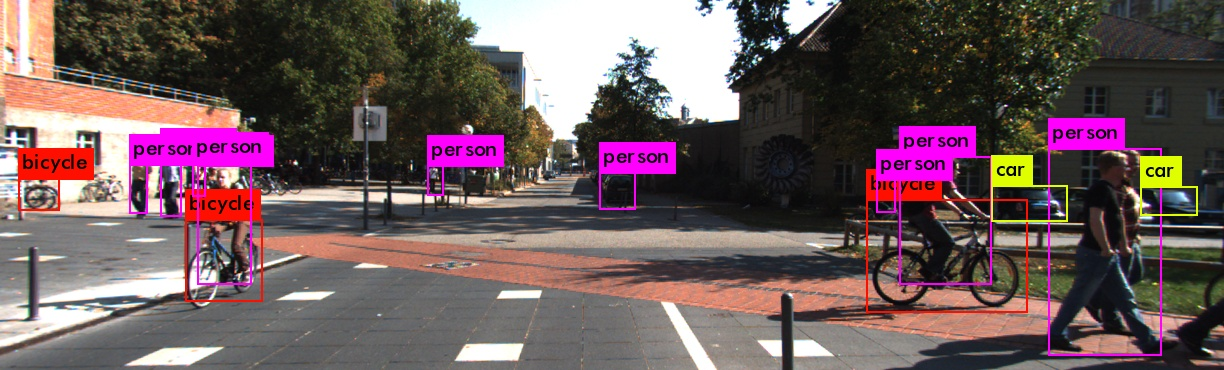
\includegraphics[width=\textwidth]{img/object-detection/kitti-2.jpg}
		\caption{Object detection on Karlsruhe Institute of Technology \textit{campus}. There are two detection errors on this image. In the center, two road poles and a car are labelled as a person. On the right, two persons are grouped together in one bounding box.}
		\label{fig:kitti-yolo-2}
	\end{subfigure}
	\caption[Image object detection results on \ac{kitti} dataset.]{Object detection results for the \ac{kitti} dataset, using \ac{yolo}v3 with a confidence threshold of 30\%, trained for the \ac{coco}'s image dataset. With the specifications present on Table~\ref{tab:computer-specs}, a 1.3 to 1.8 \ac{fps} were registered when classifying the images.}
	\label{fig:kitti-object-detection}
\end{figure}


\subsubsection{Experimental Data acquired}
Exemplary results of the object detection method applied to the experimental data gathered on a \ac{msl} robotic football field, at the \acf{irislab}, are presented on Figure~\ref{fig:experimental-object-detection}. The confidence threshold of \ac{yolo} is set to 30\% and with the specifications present on Table~\ref{tab:computer-specs}, a 1.1 to 1.4 \ac{fps} were registered when classifying the images.

Since experimental data was stored on raw format, as detailed on Section~\ref{sec:calibration:extrinsic}, de-Bayering and rectification of the raw image must be done, using the \texttt{image\_proc} package, before sending the data to the \texttt{Darknet} framework.

On the left sub-figure,~\ref{fig:experimental-yolo-2}, image object detection is done on ground-truth camera data. Objects on the background are detected, even if faraway from the camera ($\approx\SI{14}{\meter}$) and out of focus (see Sub-Section~\ref{subsec:calibration:dof-and-calibration-object}). A human dummy is classified as a person and a knob is mistakenly labelled as a sports ball. The chair and the television monitor are correctly classified, but their bounding boxes dimension are smaller than they should be, because of partial occlusion.
On the right sub-figure,~\ref{fig:experimental-yolo-1}, calibrated data is used for image detection. Objects on the front are detected: a sports ball, a chair and a person. The last two ones are detected with good bounding box accuracy, even if occluded. On the background, no objects are detected, since the objects detected on sub-Figure~\ref{fig:experimental-yolo-2} are occluded. 

\begin{figure}[!ht]
	\centering
	\begin{subfigure}[t]{0.45\textwidth}
		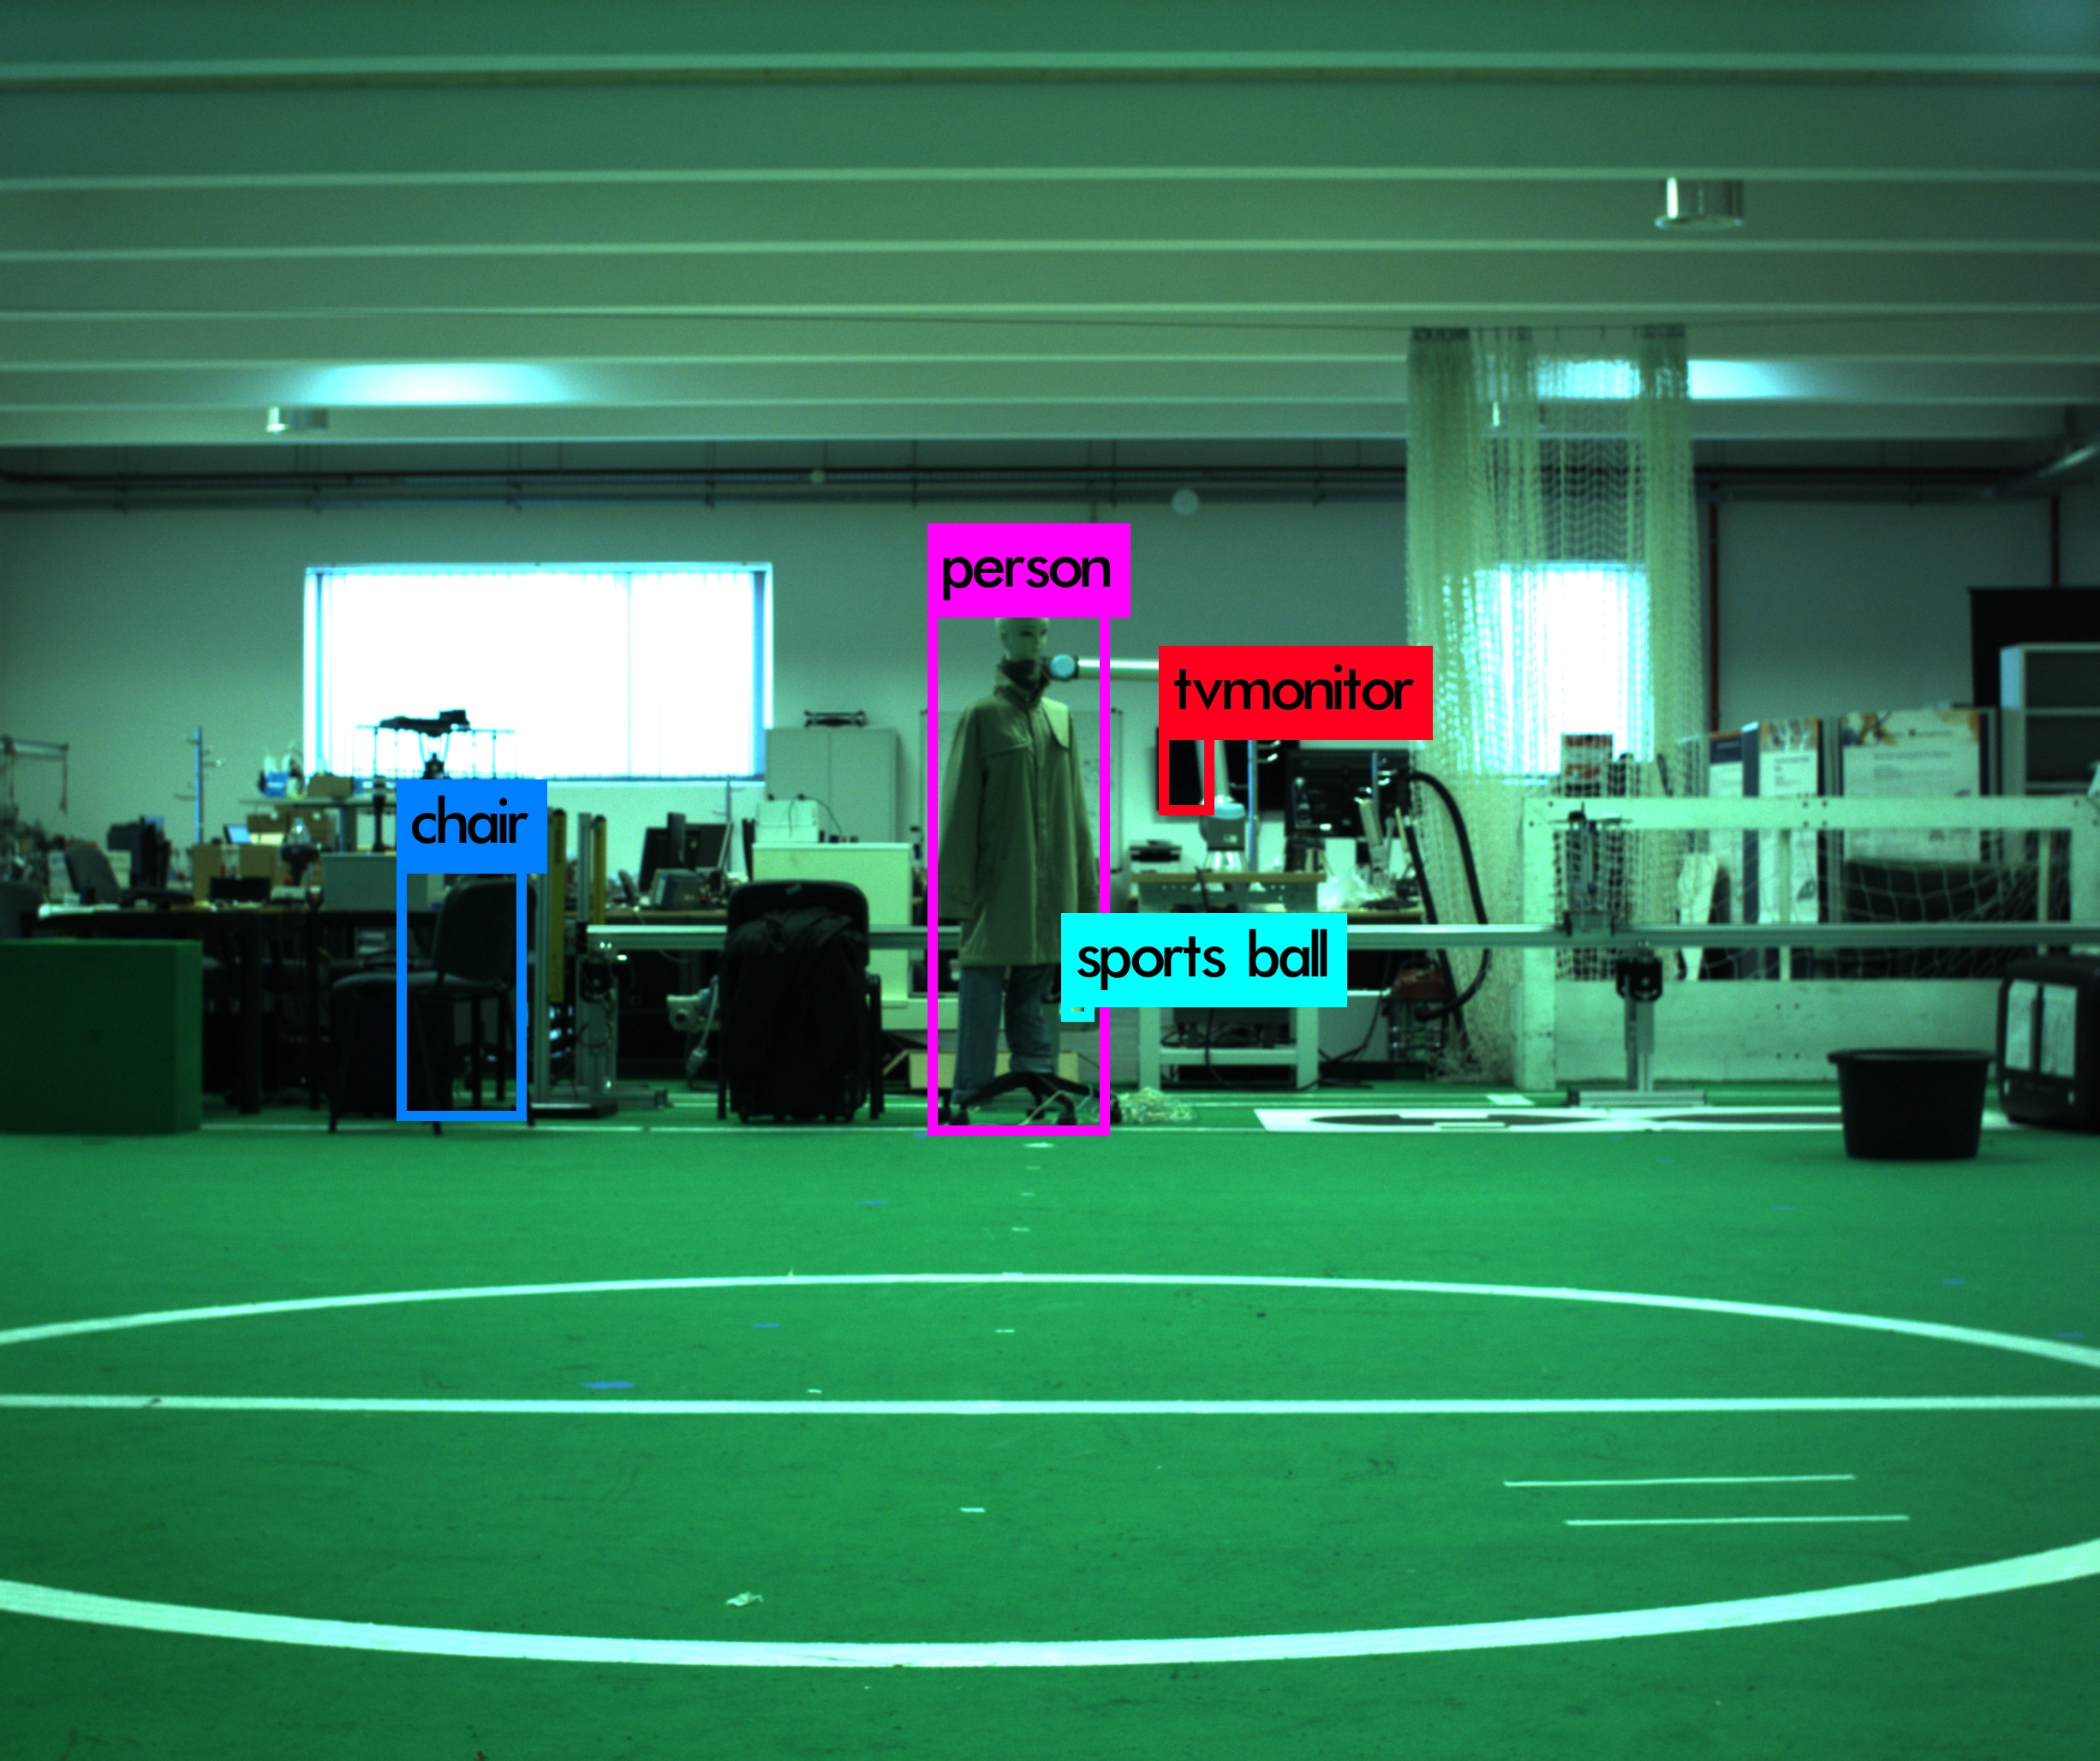
\includegraphics[width=\textwidth]{img/object-detection/experimental-2.jpg}
		\caption{}
		\label{fig:experimental-yolo-2}
	\end{subfigure}
	\qquad
	\begin{subfigure}[t]{0.45\textwidth}
		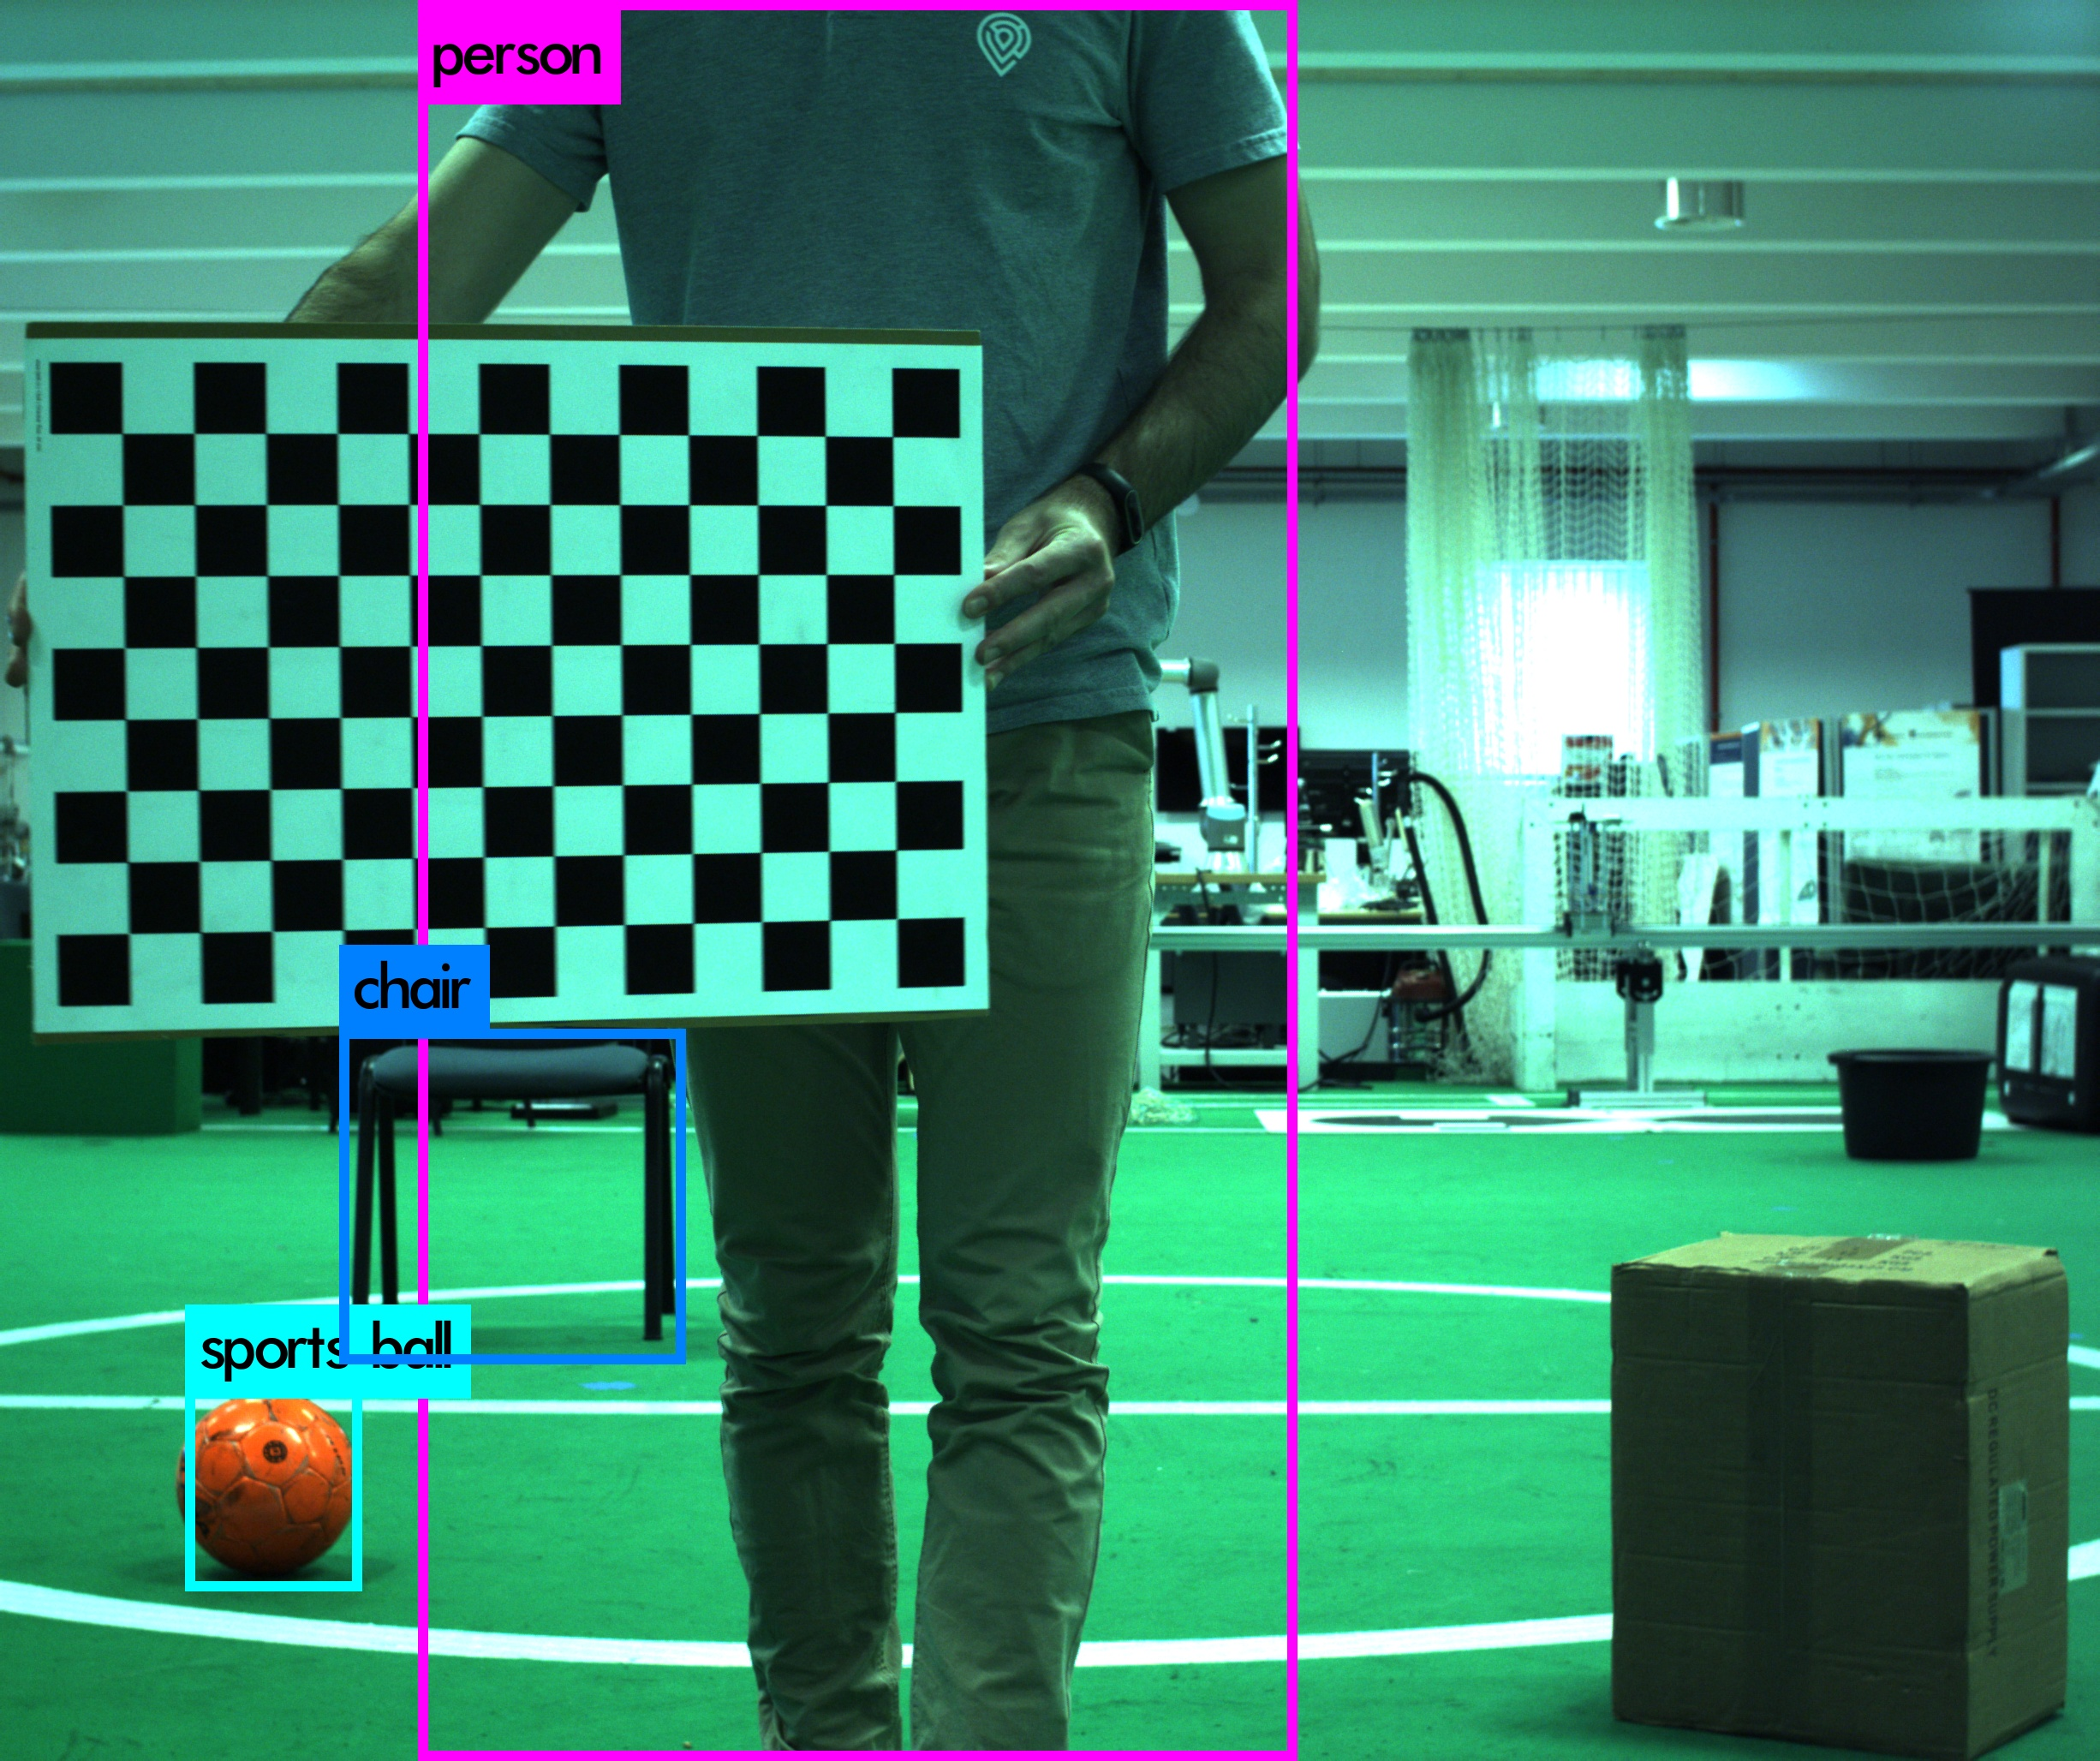
\includegraphics[width=\textwidth]{img/object-detection/experimental-1.jpg}
		\caption{}
		\label{fig:experimental-yolo-1}
	\end{subfigure}
	\caption[Image object detection, using \ac{yolo}v3 on our experimental dataset.]{Object detection results for the experimental data gathered on a \ac{msl} robotic football field, at \ac{irislab}. \ac{yolo}v3 is used with a confidence threshold of 30\% and trained for the \ac{coco}'s image dataset. With the specifications present on Table~\ref{tab:computer-specs}, a 1.1 to 1.4 \ac{fps} were registered when classifying the images. Note that since the data was stored on a raw format, de-Bayerization and rectification need to be performed by \texttt{image\_proc} \ac{ros} package before the RGB images are feed to the \texttt{Darknet}. In sub-Figure~\ref{fig:experimental-yolo-2}, a human dummy is detected as a person and a knob is confused with a sports ball. On the back, the tv monitor is correctly classified, but the bounding box is smaller, since it is occluded by the robotic arm. In sub-Figure~\ref{fig:experimental-yolo-1}, despite the occlusion of the chair and person, \ac{yolo} is capable of recognizing them both with accuracy.}
	\label{fig:experimental-object-detection}
\end{figure}

\subsection{Outcomes}
Our tests with image object detection, in conjunction with \texttt{darknet-ros}, show that the tools chosen can correctly detect the objects of interest on image and that its results can be published as messages on the \ac{ros} network, enabling other nodes to access it.

Therefore we have the first (rigid body transformation between \ac{lidar} and camera) and the second (image object detection) pre-requisites for detecting \acp{roi} on the point cloud from \acp{roi} detected on the image.

\section{Correspondences between objects in image and point-cloud}
\label{sec:object-detection:correspondences-image-point-cloud}
An experimental setup with an intrinsically calibrated camera and \ac{lidar}, on which their rigid body transformation is known\footnote{The method used to determine this rigid body transformation on our experimental dataset is outlined on Section~\ref{sec:calibration:extrinsic}. Chapter~\ref{chapter:calibration} details all the calibration procedures that are pre-required for this section. For \ac{kitti} dataset, such transformations are already given.}, allows data conversion between its two coordinate frames, as shown previously in Chapter~\ref{chapter:sensor-fusion}. 

Matching the camera's \acp{roi} with \ac{lidar}'s require converting the data to a common coordinate frame between the two sensors and then using a matching algorithm to select the point cloud points that correspond to the classified object on the image.

Determining the point cloud's \ac{roi} from the image bounding boxes implies establishing a $2D \leftrightarrow 3D$ correspondence between the data, that is used to match \acp{roi} on the two sensors. Similar to the methods for fusing different sensory data on Chapter~\ref{chapter:sensor-fusion}, two solutions based on the same principle are possible:

\begin{enumerate}
	\item The 2D pixels are converted to a 3D ray, referenced on the \ac{lidar} coordinate frame. This method uses a technique of ray-casting, computing the rays from the camera sensor center that pass through the pixel coordinates;
	\item The 3D points registered by the \ac{lidar} are projected to the image pixels plane, ``converting a two-dimensional \ac{roi} to a tridimensional \ac{roi}, A tridimensional bounding box is estimated and drawn, for visualization purposes, on the point cloud. 
\end{enumerate}

In this section, the implementation of both methods is presented, along with their results and a brief comparison. This section explains the implementation for computing the point cloud bounding boxes, by using the information of the image bounding boxes obtained with \ac{yolo}, as detailed on Section~\ref{sec:object-detection:image}. The results for every stage of the processing chain are also given.


\subsection{\texttt{Darknet-ros} Package Limitations and Contributions}
\label{subsec:object-detection:darknet-contribution}
\texttt{Darknet-ros} encapsulates the \texttt{Darknet} framework and allows its connection with other nodes on a \ac{ros} network. Excluding its interface for \ac{nn} configuration (\ac{nn} model and weights) and data input topics, that are detailed on~\cite{MarkoBjelonic}, \texttt{darknet-ros} provides 3 output topics:

\begin{enumerate}
	\item \texttt{found\_object}: a standard integer message that indicates the number of objects found by the \texttt{Darknet} framework when running the desired \ac{nn} model;
	\item \texttt{detection\_image}: A \ac{ros} image topic, similar to its input image topic, but with the detection bounding boxes drawn;
	\item \texttt{bboxes}: a custom message topic that contains a header with metadata and an array of bounding boxes detected on the image. Each bounding box element of this array indicates its class, ID, probability and the minimum and maximum points that define the image bounding box for that object;
\end{enumerate}

For this work, precise synchronization between the point cloud and \texttt{darknet}'s outputs is required. However, \texttt{darknet-ros}' does not provide an interface with such functionality, lacking information to synchronise the \texttt{found\_objects} topic with other topics.

To mitigate this problem, we propose an improvement on \texttt{darknet-ros} package. Our proposal consists on defining a custom message for \texttt{found\_objects} topic that additionally to the standard integer indicating the found objects' number, also contains a header with the time stamps and frame id for synchronization. The \texttt{darknet-ros} core code was also changed to publish this new message type under \texttt{found\_objects} topic, ensuring also backwards compatibility.

Those changes were later submitted to the original author of \texttt{darknet-ros}, which were accepted and merged with the publicly available source code~\cite{MarkoBjelonic}.


\subsection{Ray Casting}
\label{subsec:object-detection:ray-casting}
The first implemented algorithm to match image and point cloud \acp{roi} involves a technique of ray casting, i.e., casting a ray from the camera center that passes thought the desired pixel, projecting it from the two-dimensional image representation to a three-dimensional, that is suited for comparison with \ac{lidar} data.

After data conversion from one coordinate frame to the other, using the rigid body transformation determined on Section~\ref{sec:calibration:extrinsic}, ray-casting allows the determination of 4 lines that delimit a 3D section of the point cloud, by casting the corners of the image bounding box. These 4 lines, transformed to the \ac{lidar} coordinate frame, define the boundaries of an infinite rectangular pyramid, with its vertex on the \ac{lidar} center. Considering a near and far parallel cut planes that are perpendicular to the pyramid orientation, a pyramidal frustum is obtained (see Figure~\ref{fig:pyramid-frustum}), containing all the point cloud points that are part of the tridimensional \ac{roi} for the object detected.  

\begin{figure}[H]
	\centering
	\def\svgwidth{0.3\columnwidth}
	\graphicspath{{img/image-object-to-point-cloud/}}
	\includesvg{img/image-object-to-point-cloud/pyramid-frustum}
	\caption[Representation of a pyramid frustum.]{Pyramid Frustum. The gray section corresponds to the pyramid frustum volume between the near and far plane on the boundaries defined by the pyramid.}
	\label{fig:pyramid-frustum}
\end{figure}

Performing a frustum segmentation on the point cloud requires four steps:

\begin{itemize}
	\item Back-project the pixels to rays, defining the boundaries of the point cloud;
	\item Compute the pure rotation coefficients that align the \ac{lidar} coordinate frame to the coordinate frame oriented to the \ac{roi};
	\item Calculate the vertical and horizontal \acf{fov} of the pyramid frustum;
	\item Determine the limits of the near and far cut planes.
\end{itemize}

\subsubsection{Back-project the pixels to rays}
Projecting pixels to a ray (also called back projection) is the inverse process that is used to create an image on a camera\footnote{A camera projects the world points to a two-dimensional plane. See Sub-Section~\ref{subsec:sota:camera-geometry}}. The projection matrix defined in Equation~\eqref{eq:camera_transform_full}, if inverted, may be used to calculate the transformation matrix that  back projects pixels into rays.

Since on our implementation, the transformation between different coordinate frames is done separately from the back-projection algorithm, the image pixels are already defined on the camera's coordinate frame. Therefore, the joint rotation and translation matrix, $\begin{bmatrix} R|t \end{bmatrix}$, is equal to the identity and a zero column vector, respectively, and does not need to be accounted for.

Following Hartley's and Zisserman's book~\cite{mvg_book}, our back-projection operation degenerates to computing the inverse of the intrinsic camera matrix, $K$, and multiply that inverse by the pixel coordinates referenced in affine coordinates, detailed in Equation~\eqref{eq:back-projection}. The rotation and translation to convert the rays from the camera's coordinate frame to \ac{lidar}'s are applied after the ray-casting operation.

\begin{align}
	\label{eq:back-projection}
	\begin{bmatrix}
		X \\
		Y \\
		Z
	\end{bmatrix}
	 & = K^{-1} 
	\begin{bmatrix}
		u \\
		v \\
		1
	\end{bmatrix}
\qquad , \quad
	K = 
	\begin{bmatrix}
		f_x & 0 & c_x \\
		0 & f_y & c_y \\
		0 & 0 & 1.0
	\end{bmatrix}
\nonumber \\	 
	&  = 
	\begin{bmatrix}
	\frac{1}{f_x} & 0 & -\frac{c_x}{f_x} \\
	0 & \frac{1}{f_y}  & -\frac{c_y}{f_y} \\
	0 & 0 & 1.0 
	\end{bmatrix}
	\begin{bmatrix}
		u \\
		v \\
		1
	\end{bmatrix}
\end{align}

\subsubsection{Rotation from the \ac{lidar} coordinate frames to the bounding boxes' coordinate frame}
The rotation of the \ac{lidar} coordinate frame to each of the bounding boxes coordinate frames is obtained by calculating the angle between the two rays: the ray from the camera center to the image bounding box center and the ray from the camera center to the image center. 

Let $B^\text{center}$ be the image bounding box center, which can be calculated using Equation~\eqref{eq:bboxes-pixel-center} and $C^\text{center}$ be the image center, that corresponds to the intrinsic camera parameters $c_i, \forall i \in \{x, y\}$, as denoted in Equation~\eqref{eq:image-pixel-center}.

\begin{equation}
	\label{eq:bboxes-pixel-center}	
B^\text{center} = \left(\frac{x^{\text{bounding box}}_{min} + x^{\text{bounding box}}_{max}}{2}, \frac{y^{\text{bounding box}}_{min} + y^{\text{bounding box}}_{max}}{2},\right)
\end{equation}

\begin{equation}
\label{eq:image-pixel-center}
C^\text{center} = (c_x, c_y)
\end{equation}

%Considering that the representation of a generic point $P = (x, y, z)$ in affine coordinates is given by $P_\text{affine} = \left[P | 1\right]^T$, where $T$ represents the matrix transpose, and consider that in this case, $P \in \{B^\text{center}, C^\text{center} \}$. 
Denote  the ray projected by the camera origin that passes through the pixels defined by the points $B^\text{center}_\text{affine}$ and $C^\text{center}_\text{affine}$, as $\vec{b}$ and $\vec{c}$, respectively, where $\vec{b}$ and $\vec{c}$ are determined using Equation~\eqref{eq:back-projection}, that $\vec{b} = K^{-1} \times B^\text{center}_\text{affine}$ and $\vec{c} = K^{-1} \times C^\text{center}_\text{affine}$.

By applying the rigid body transformation between the camera and the \ac{lidar} determined in Section~\ref{sec:calibration:extrinsic}, let us define vector $\vec{b'}$ and $\vec{c'}$ as the vectors $\vec{b}$ and $\vec{c}$, referenced on the \ac{lidar} coordinate frame, respectively.

Then, the rotation of the \ac{lidar} coordinate frame to a new frame oriented to the bounding box can then be obtained by calculating the quaternion that defines the angle of rotation between vector $\vec{c'}$ and $\vec{b'}$~\cite{mvg_book}. The rotation transformation can be denoted as $\mathbf{q}_{c'b'}$, which is capable of projecting a line from the coordinate frame of the bounding box, $b'$, to the \ac{lidar} coordinate frame, $c'$. Afterwards, the quaternion can be converted to a rotation matrix~\cite{Dai2015, mvg_book}, so that the rotation can be applied together with order rotations already obtained.

\subsubsection{Horizontal and Vertical \ac{fov} of the pyramidal frustum}
The horizontal and vertical \ac{fov} are determined on the image plan. First, the angle between the image center and each of the bounding box limits (upper and lower) are calculated for the two dimensions, $x$ and $y$. Then, the difference between the upper and lower angles is computed to obtain the \ac{fov} on that axis.

Let $\theta^\text{upper limit}_i$ denote the upper limit of the image bounding box, on the generic $i$ axis, that can be replaced by $x$ or $y$, and $\theta^\text{lower limit}_i$ represent the lower limit of that same axis. Consider the image axis origin to be at the center of the image and the \ac{fov} of the bounding box can be defined by $\Theta^\text{FOV}_i$ on Equation~\eqref{eq:image-fov}, for that same generic axis $i$.

\begin{equation}
	\label{eq:image-fov}
	\Theta^{FOV}_i = \theta^\text{upper limit}_i - \theta^\text{lower limit}_i, \qquad \forall i \in \{x, y\}
\end{equation}

With some trigonometry and camera geometry\footnote{Camera geometry is detailed on sub-Section~\ref{subsec:sota:camera-geometry}. Figure~\ref{fig:pinhole_camera_model} might be interesting revisiting before continuing.} one can see that:

\begin{align}
	\theta^\text{upper limit}_i = \tan\left(\frac{\max(i)}{f_i}\right), \qquad i \in \{x, y\} \\
	\theta^\text{lower limit}_i = \tan\left(\frac{\min(i)}{f_i}\right), \qquad i \in \{x, y\} 
\end{align}

\subsubsection{Determine the near and far cut planes limits}
The Near and Far Cut Planes may be defined by the data and \ac{lidar} constraints. Following the datasheet of the VLP-16~\cite{vlp16}, the \ac{lidar} used on the experimental setup, and HDL-64~\cite{VelodyneHDL64}, the \ac{lidar} used on the \ac{kitti} dataset, the Near Cut Plane is defined as \SI{1}{\meter}, since the \acp{lidar} cannot detect smaller distances.

Due to point cloud data scarcity, both on the experimental and  \ac{kitti} dataset, a Far Plane of \SI{30}{\meter} is enough to guarantee that all the objects of interest on the \ac{fov} are present.

\subsubsection{Implementation}
Using the constrains and methods detailed before, a \ac{ros} node, \texttt{image\_bbox\_to\_point\_cloud\_node}, is written to perform frustum filtering on the point cloud using the image bounding boxes determined by \texttt{darknet-ros}. The node diagram is shown on Figure~\ref{fig:ros-graph-frustum}, in Appendix~\ref{appendix:appendix-diagram}, where the node \texttt{Kitti\_dataset} is a \texttt{rosbag} player and \texttt{darknet-ros} is the node described in Section~\ref{sec:object-detection:image}, responsible for image object detection. \texttt{Rviz} is the \ac{ros} visualizer, configured to show the transformations between the coordinate frames, the original point cloud and the frustum filtered point cloud.

%\begin{figure}[t]
%	\centering
%	\def\svgwidth{\columnwidth}
%	\graphicspath{{img/image-object-to-point-cloud/}}
%	\includesvg{img/image-object-to-point-cloud/frustum-print}
%	\caption[\ac{ros} node graph for the point cloud frustum filter algorithm.]{\ac{ros} node graph corresponding to the implementation of the Point Cloud Frustum Filter node from the image bounding boxes.}
%	\label{fig:ros-graph-frustum}
%\end{figure}


This node is implemented using \ac{pcl} frustum filter algorithm and Eigen library. Eigen is a C++ library for linear algebra, matrix and vector operations and geometric transformations, among other features~\cite{Eigenv3}. The pose of each of the bounding boxes is also computed, either towards the \ac{lidar}'s and the \ac{pcl}'s frustum algorithm coordinate frame. 

Several alternatives to the methods described above (for \ac{fov} calculation, determine the \ac{lidar} rotation, for example) have been implemented, but are not going to be described here. Several auxiliary functions (for debugging, visualization and computing other features) will also not be addressed, since they require a more in depth explanation of the implementation, that was no interest for such document. 


\subsubsection{Results}
Applying the frustum filtering methodology described on the sub-sections above to the point cloud data can be seen on Figure~\ref{fig:bbox-correspondences-on-kitti}. The dark grey points correspond to the original point cloud, \texttt{velodyne\_points}, and the orange points to the frustum filtered point cloud, \texttt{frustum\_filtered\_point\_cloud}.

The red arrows represent the pose of each of the objects \acp{roi} and the yellow arrows the pose of those objects on the frustum filter coordinate frame, which differs from the Velodyne \ac{lidar} coordinate frame. Although the Velodyne \ac{lidar} coordinate frame is z upwards, y leftwards and x forward\footnote{Velodyne \ac{lidar} coordinate frame on \ac{kitti} dataset can be seen better in Figure~\ref{fig:kitti-tf-frames} on sub-Section~\ref{subsec:calibration:kitti-comparison} or on \ac{kitti}'s paper~\cite{Geiger2013a}.}; the \ac{pcl} frustum filter coordinate frame is y upwards, z rightwards and x forward.

\begin{figure}[!ht]
	\centering
	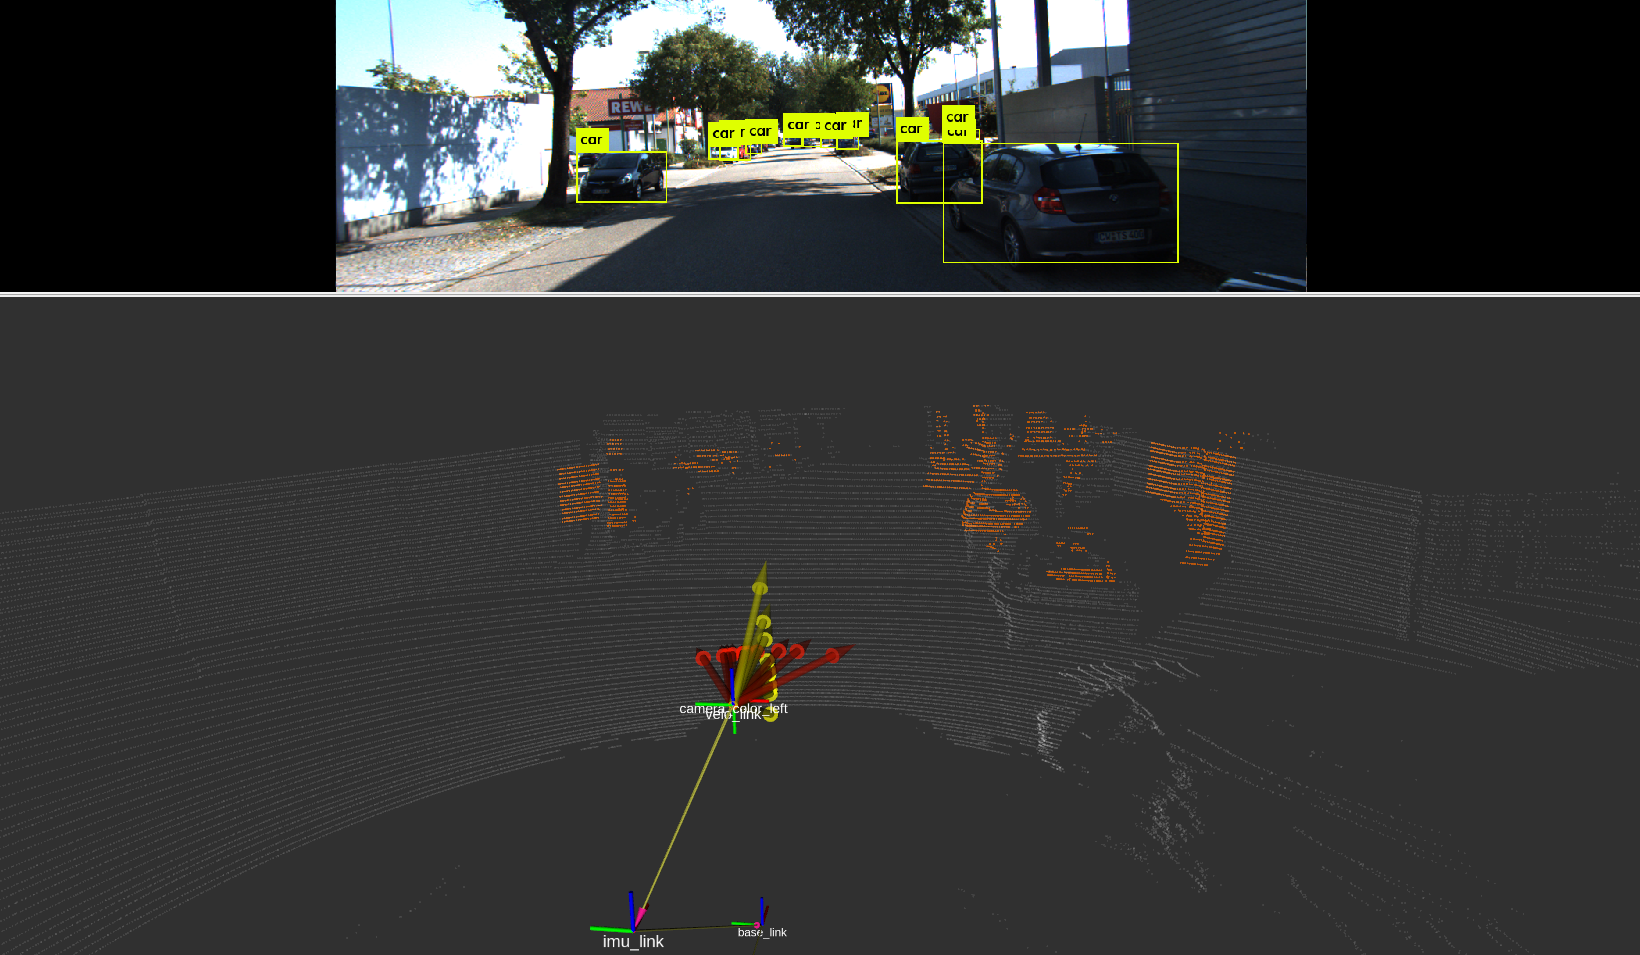
\includegraphics[width=0.8\textwidth]{img/image-object-to-point-cloud/bbox_correspondences_on_kitti.png}
	\caption[Points corresponding to the image objects' bounding boxes, using the frustum filtering correspondences algorithm.]{Pyramidal Frustum filtering of \acp{roi} given by the image bounding boxes on \ac{lidar} data. The dark grey points correspond to the unfiltered \ac{lidar} point cloud and the orange points to the ones selected by frustum filtering. One can see that there is a discrepancy between the objects of interest on the point cloud (cars) and the selected \acp{roi} by the algorithm. The red arrows point to each of the \acp{roi} on the \ac{lidar} coordinate frame and the yellow arrows point to the \acp {roi} on the \ac{pcl}'s frustum filter algorithm coordinate frame.}
	\label{fig:bbox-correspondences-on-kitti}
\end{figure}

The results shown on Figure~\ref{fig:bbox-correspondences-on-kitti} are not as anticipated. Mismatches between the bounding boxes on the image and \acp{roi} selected by the frustum filter are not coincident. Analyzing the unfiltered (gray points) and the filtered point cloud (orange points), one can notice that some regions of the dark grey point cloud that correspond to the cars (that are detected on the image), are not considered a \ac{roi} and therefore are not filtered by the algorithms implemented and are not part of the filtered point cloud. Also, in contrast, some regions that have not been considered as \acp{roi} on the image are selected on the point cloud.

A mismatch on determining the correspondences between the \acp{roi} on the image and \ac{lidar} has been made, that can either be from the coordinate frames conversion, calculation of the \ac{lidar} rotation and \ac{fov} determination or by a combination of errors/imprecisions made in one of these steps. The implementation requires some third party libraries, such as \ac{pcl}, \ac{opencv} and Eigen, to be integrated in order to filter the point cloud, which might also be the source of the problems.

The implementation was thoroughly debugged but the cause of the mismatch was not found. Therefore, a simpler algorithm to match the \acp{roi} between camera and \ac{lidar} was developed, to fulfill the thesis objective of computing correspondences between image and point cloud objects.


\subsection{Projecting \ac{lidar} points to the image}
\label{subsec:object-detection:projection-correspondences}

The alternative method to establish correspondences is similar to the one used for Sensor Fusion, detailed in Chapter~\ref{chapter:sensor-fusion}. The difference between the implementation on the latter chapter and this is that instead of comparing if the projected \ac{lidar} points correspond to a pixel in the image, they must also be contained in an image bounding box. 

This approach has a few drawbacks when compared with the previously described in sub-Section~\ref{subsec:object-detection:ray-casting}, but is easier and less complex. It requires only four steps, some already implemented previously:

\begin{enumerate}
	\item Transform the \ac{lidar} point cloud from the \ac{lidar} coordinate frame to the camera's coordinate frame, as detailed in sub-Section~\ref{subsec:calibration:calibration-method}. Similar to the conversion in Chapter~\ref{chapter:sensor-fusion}, the coordinate conversion frame is the rigid body transformation determined in Section~\ref{sec:calibration:extrinsic}.;
	\item Project the \ac{lidar} point cloud points to the camera's image two-dimensional planes, using the methodology detailed in sub-Section~\ref{subsec:sensor-fusion-lidar-to-camera};
	\item Check if the projected point cloud points correspond to image pixels inside of image bounding boxes. If true, save the index of the point cloud point;
	\item Using \ac{pcl}'s Extract Indices filter, a new point cloud is created from the original, containing the indexes selected on the previous step.
\end{enumerate}

However, using this method, every point of the point cloud is treated independently of the others. Since the point cloud is not organised, causing the spatial relation of the \acp{roi} on point cloud to not be preserved, the information of the detected objects on image (class, probability) obtained through the image object detection of Section~\ref{sec:object-detection:image} is harder to transfer to the corresponding points on the point cloud.


\subsubsection{Implementation}
The methodology chosen builds upon the implementation detailed on Section~\ref{sec:object-detection:image}. A new node, \texttt{correspondences\_finder}, responsible for extracting the indices and  publishing a filtered point cloud, is implemented. The \texttt{filtered\_point\_cloud} contains all the points that belong to the \acp{roi} correspondent to the image bounding boxes. 

The node is agnostic about the objects that are identified by the image object detection algorithms, considering only the bounding box dimensions and ignoring its class and confidence. Considering the mathematical notation of a bounding box as $bbox^i_j$, where $i$ corresponds to the bounding box index on \texttt{darknet-ros}' \texttt{bboxes} message and $j$ the coordinate of the bounding box, such as $j \in \{x, y\}$. Let also the number of the bounding boxes index be denoted as $\text{found\_object}$. A correspondence is made when the point cloud projection coordinates are such that a given point cloud point $P = (p_x, p_y,p_z)$ verifies Equation~\eqref{eq:correspondences-condition}.

\begin{align}
	\label{eq:correspondences-condition}
	\forall i \in & [0, \ldots, \text{found\_object}], \nonumber \\ 
			& \exists P \in [\min(bbox^i_x), \max(bbox^i_x)] \cap [\min(bbox^i_y), \max(bbox^i_y)] 
\end{align}

The node diagram is presented on Figure~\ref{fig:correspondences-finder-standalone}, on Appendix~\ref{appendix:appendix-diagram}. Similar to Figure~\ref{fig:bbox-correspondences-on-kitti}, the implementation requires the usage of \texttt{Darknet-ros} to compute the image bounding boxes. The two alternatives are completely interchangeable, publishing the same type of message (a point cloud) and receiving the same inputs: the original \ac{lidar} point cloud, coordinate frame transforms and \texttt{darknet-ros} bounding boxes message and the number of detected objects.

%\begin{figure}[!ht]
%	\centering
%	\def\svgwidth{\columnwidth}
%	\graphicspath{{img/image-object-to-point-cloud/}}
%	\includesvg{img/image-object-to-point-cloud/correspondences-finder-standalone-print}	
%	\caption[\ac{ros} node diagram for the estimation ob point cloud bounding box from image bounding boxes of objects of interest.]{\ac{ros} node diagram for \texttt{correspondences\_finder} implementation. It uses \texttt{Darknet-ros} to compute the image bounding boxes and a \texttt{rosbag} player to publish \ac{kitti} dataset data. The node publishes a point cloud message, \texttt{filtered\_point\_cloud}, containing the \ac{lidar} \acp{roi}' points, selected from the input point cloud, \texttt{velodyne\_points}.}
%	\label{fig:correspondences-finder-standalone}
%\end{figure}

\subsubsection{Results}
On Figure~\ref{fig:projected-correspondences}, the results caused by applying the \texttt{correspondences\_finder} node are presented in lilac. The top part of the image presents the camera feed and the bottom the point cloud, with the relevant TF coordinate frames also visible. The  dark gray points represent the original \ac{lidar} data. 

Analyzing the results, we conclude that the objects of interest (cars, on Figure~\ref{fig:projected-correspondences}) are filtered, and part of the point cloud that contains the \acp{roi} marked in lilac. In every \ac{roi}, however, some outlier points are also selected. This is because the image bounding boxes being rectangular, which results on non-optimal bounding boxes dimensions, causing the appearance of outliers when correspondences between the \ac{lidar} and camera data are made.

These outliers correspond to objects nearby of the detected object or to objects that occlude it. Normally, it contains a part of the background and the floor. Such outliers pose a problem, since points that do not belong to the object are being selected as part of it, and must be solved before any bounding box estimation can take place. Nevertheless, we consider the correspondences' detection to be correct and the results satisfactory.


\begin{figure}[!ht]
	\centering
	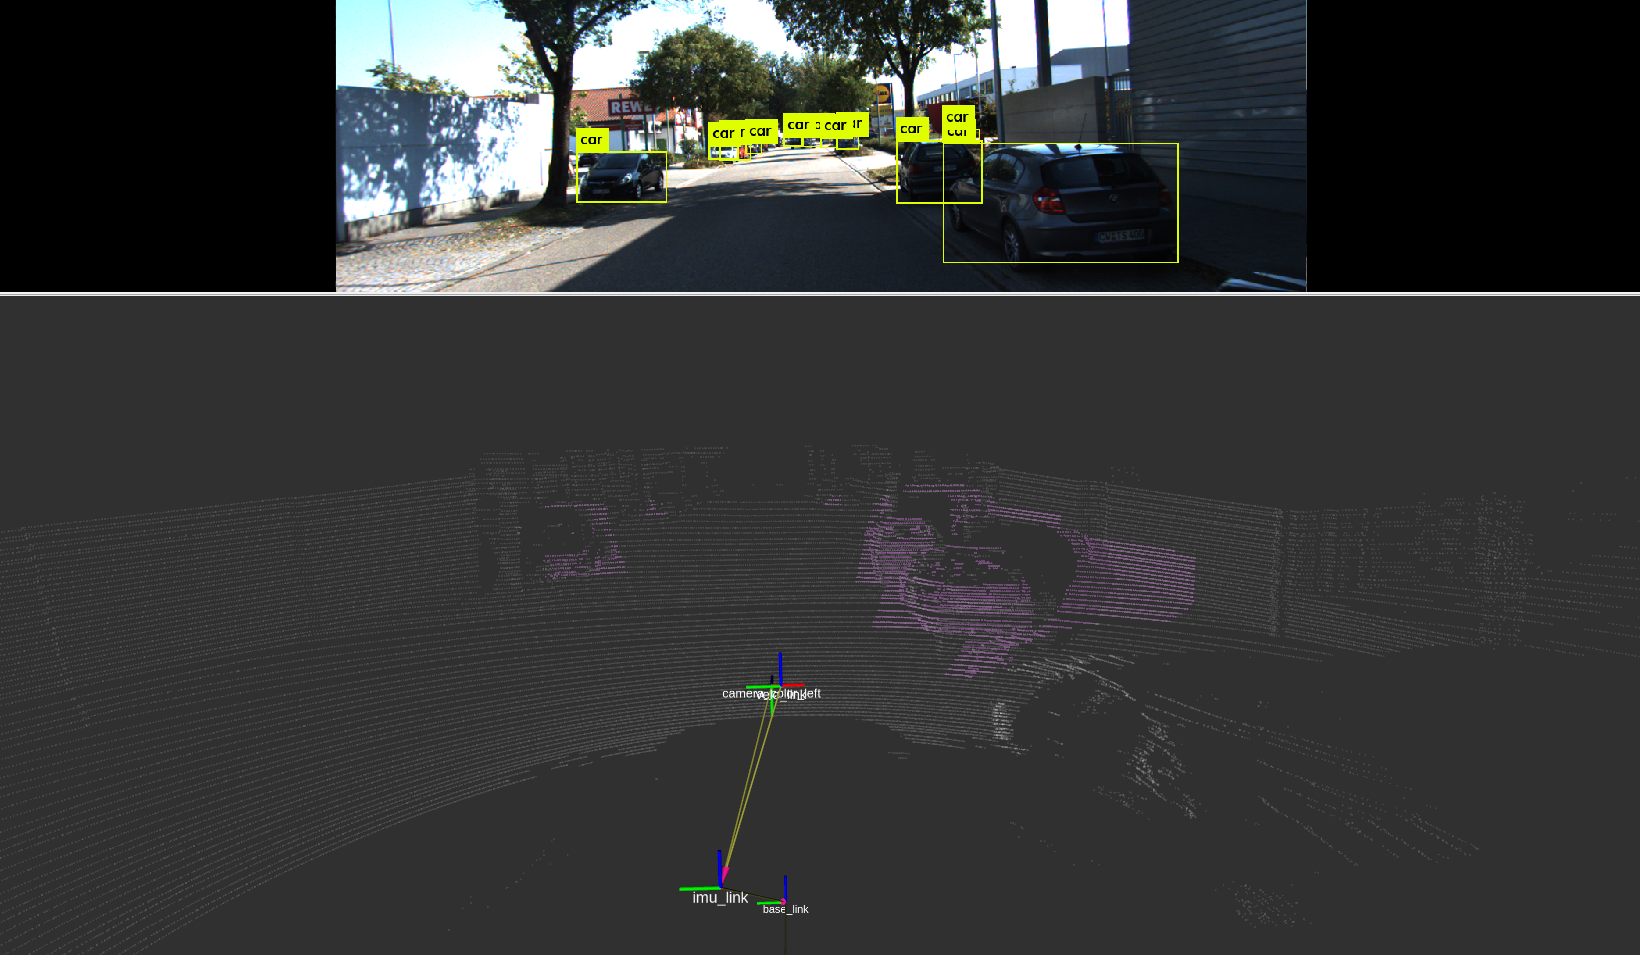
\includegraphics[width=0.8\textwidth]{img/image-object-to-point-cloud/projected_correspondences.png}
	\caption[Points corresponding to the image objects' bounding boxes, using the $3D \rightarrow 2D$ correspondences algorithm.]{Correspondences between the image bounding boxes and point cloud \acp{roi}. The dark grey points correspond to the unfiltered \ac{lidar} point cloud and the lilac points to the ones selected by the \texttt{correspondences\_finder} node, using the projection algorithm detailed. One can see that the cars that are detected on the image are filtered and marked by the algorithm. On those regions, some outliers are also present due to the bounding boxes being non-optimal to enclose the object dimensions.}
	\label{fig:projected-correspondences}
\end{figure}

\subsection{Comparison between the two methods}
The results of the two approaches can be compared on Figure~\ref{fig:rois-matching-comparison}. In orange, the results of Sub-Section~\ref{subsec:object-detection:ray-casting}, based on ray-casting and data conversion from the camera to \ac{lidar}; and in lilac, the results of Sub-Section~\ref{subsec:object-detection:projection-correspondences}, based on projecting the \ac{lidar} points to the image plan and verifying which points laid inside the image bounding boxes limits.


\begin{figure}[!ht]
	\centering
	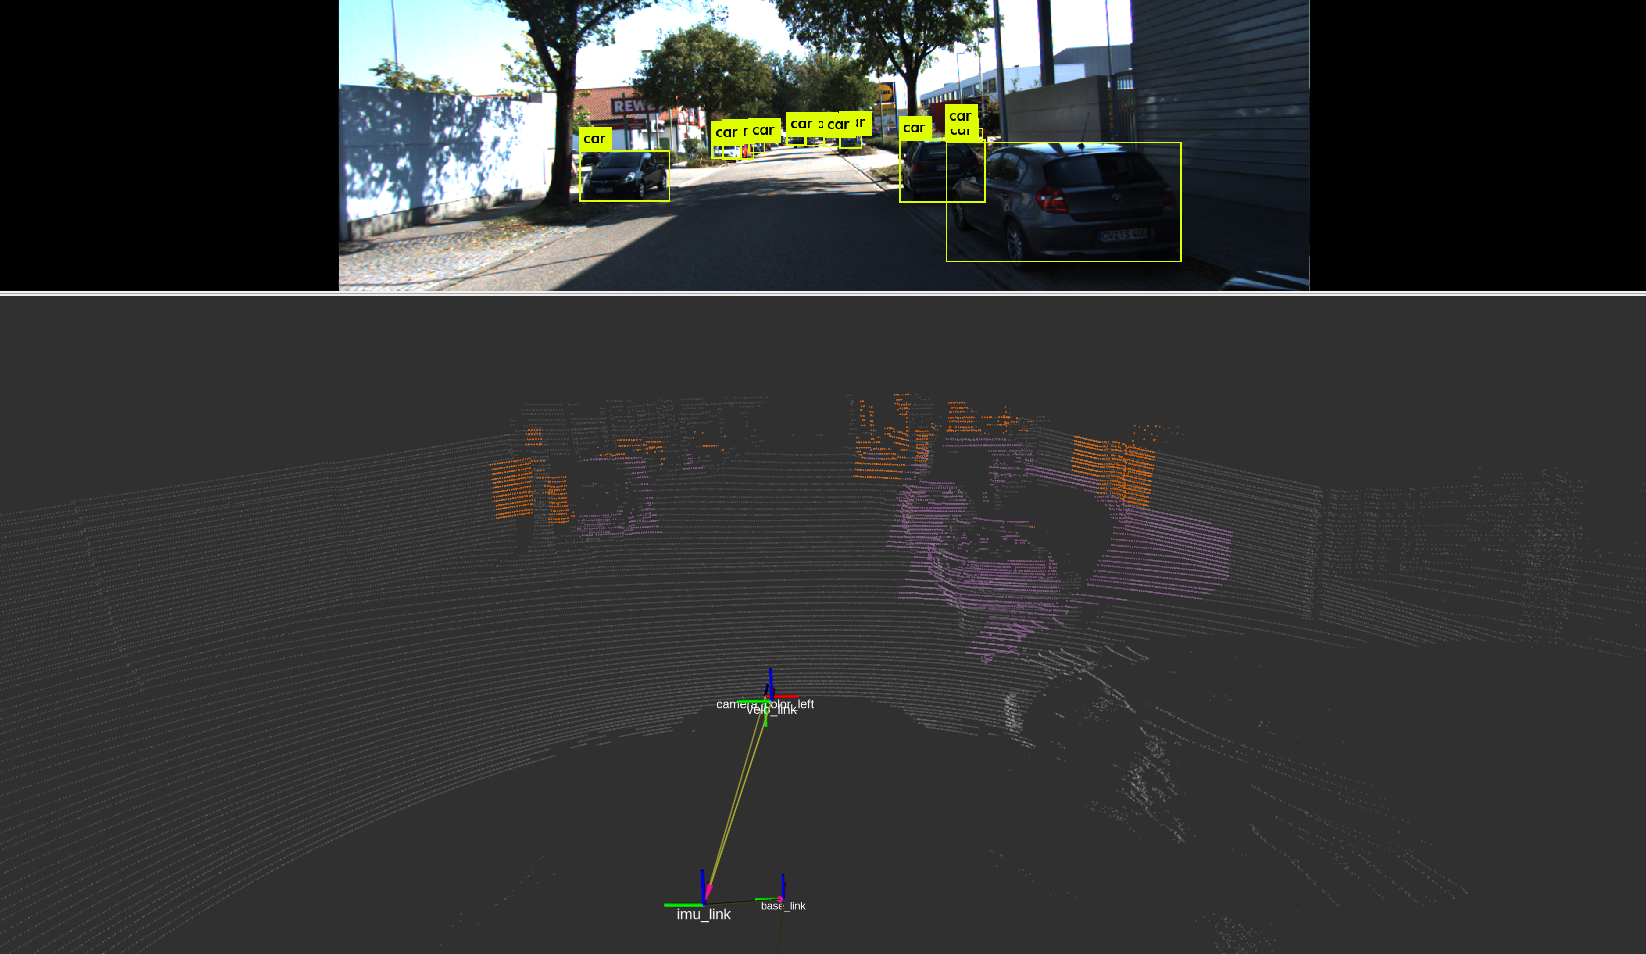
\includegraphics[width=0.8\textwidth]{img/image-object-to-point-cloud/rois-comparison.png}
	\caption[Comparison between the $3D \rightarrow 2D$ and frustum filtering correspondences algorithm results.]{Comparison between the point cloud's \acp{roi} selected with the two algorithms: in lilac, using the \texttt{image\_bbox\_to\_point\_cloud\_node} (detailed in Sub-Section~\ref{subsec:object-detection:ray-casting}); and in orange, using the \texttt{correspondences\_finder\_node} (detailed in Sub-Section~\ref{subsec:object-detection:projection-correspondences}). On the bottom of the image, a dark gray point cloud is also presented, showing the original point cloud gathered by the \ac{lidar}. Comparing with the top part of the image, which shows the camera feed, the lilac subset of the original point cloud identifies with better accuracy the point cloud \acp{roi} that correspond to the detected objects on the image.}
	\label{fig:rois-matching-comparison}
\end{figure}

After analyzing the comparison between both algorithms on Figure~\ref{fig:rois-matching-comparison}, the solution chosen for detecting \acp{roi} on the point cloud using the image \acp{roi} represented as bounding boxes, is the one detailed in Sub-Section~\ref{subsec:object-detection:projection-correspondences}, since the results are more accurate.

\subsection{3D Bounding Boxes and \aclp{roi}}
\label{subsec:object-detection:bounding-boxes-and-roi}
Estimating a \ac{roi} on a point cloud from an image has the caveat of requiring the conversion between a 2D object (a rectangle representing a bounding box on the image) to a 3D object (a parallelepiped representing a bounding box on the point cloud). As detailed in the Chapter~\ref{chapter:sensor-fusion}, such conversion requires the estimation of one degree of freedom, depth, whose information is absent from the image.

As detailed in this chapter, we want to draw a bounding box on the point cloud using only the information of the camera. Therefore, we need to estimate the depth of the 3D bounding box that contains all the points of an object that correspond to the object of interest on the image, that was classified during the image detection procedure (see Section~\ref{sec:object-detection:image}).

To reduce mismatches and improved the accuracy of the bounding boxes, before computing them, the point cloud is filtered using a voxel filter to uniform point cloud density on the already filtered \acp{roi}. The voxelized point cloud is then feed to a clustering algorithm, to select on the points of each \ac{roi} that correspond to the actual object of interest, reducing outliers. The resulting clusters are then used as input for the bounding box estimation algorithm.


\subsubsection{Voxelization}
To reduce the number of points on the filtered point cloud (speeding up the process) and to uniform point density, \ac{pcl}'s Voxel Grid filter is used to voxelize the point cloud. \ac{pcl}'s voxel grid creates a tridimensional grid of voxels that encapsulate all the point cloud points and, for every voxel, the centroid of the points within each voxel is computed, replacing all the voxel's points with its centroid.

On our experimental datasets, a voxel grid of \SI{0.04}{\centi\meter} was used, causing a reduction of 5\% to 15\% on the filtered point cloud number of points.

\subsubsection{Clustering}
As seen in Figure~\ref{fig:projected-correspondences}, the filtered \acp{roi} contain outliers that do not belong to the object of interest detected on the image. Those outliers originate from the non-optimal image bounding box dimensions, and must be removed (or at least reduced) to ensure a good tridimensional bounding box fitting.

Since the point cloud density varies with distance, clustering will cause the distant \acp{roi} to be removed and the closer \acp{roi}, since a voxel filter has been applied, to be filtered, since the point cloud density is approximately uniform for a single object. Our implementation uses \ac{pcl}'s Euclidean Clustering algorithm, with a search method based on K-Dimensional tree\footnote{On our case, K$=3$, since the point cloud data only contains 3 euclidean coordinates: x, y, z.} for space partitioning and point cloud organization.

The Euclidean Filter uses 3 parameters:

\begin{enumerate}
	\label{enum:object-detection:cluster-parameters}
	\item \textbf{Cluster tolerance:} Maximum distance between the points of the cluster, measured using a Euclidean L2 norm. If the L2 norm between a cluster point and a candidate cluster point is greater than this parameter, the candidate point is not part of the cluster;
	\item \textbf{Minimum cluster size:} Minimum number of points, that verify the cluster tolerance condition, that are required to create a cluster. If the number of points that verify condition 1 is smaller than this number, a cluster is not created;
	\item \textbf{Maximum cluster size:} Maximum number of points, that verify the cluster tolerance condition, that can be part of a cluster. The number of points that verify condition 1 must be smaller or equal than this parameter, otherwise a cluster is not created.
\end{enumerate}

To ease the estimation of the filter parameters, \texttt{correspondences\_finder\_node} was changed to contain a \ac{ros} dynamic reconfigure server, allowing the modification of the filter parameters in real-time during program execution. 

To tune the parameters, minimum and maximum cluster size were set to 1 and 25000, respectively. Cluster tolerance was then decreased from \SIrange{10}{0.2}{\meter} with non-uniform steps until each of the clusters contain only one object. Then, the minimum cluster size was increased until only the clusters of interest remain, i.e., the clusters that correspond to the objects detected on the image bounding boxes, which results on a number of points equal $150$. With this first estimation carried, the parameters were fine-tuned, resulting on the final values for the parameters presented in Table~\ref{tab:euclidian-cluster-specs}.

\begin{table}[H]
	\centering
	\renewcommand{\arraystretch}{1.2}
	\begin{tabular}{@{}p{6cm}l@{}}
	 \toprule
	 Specification & Value \\
	 \midrule
	 Cluster Distance Tolerance & \SI{0.18}{\meter}\footnotemark \\
	 Minimum cluster size & $180$ \\
	 Maximum cluster size & $8000$ \\
	 \bottomrule
	\end{tabular}
	\caption[\ac{pcl}'s Euclidian Cluster filter parameters for \ac{kitti} dataset.]{\ac{pcl}'s Euclidean Cluster filter parameters used on our algorithms for the \ac{kitti} dataset. On \ac{kitti}'s and our data, these parameters can segment the clusters corresponding to the object while removing some outliers on the \ac{roi}. These parameters are set as the default for the \ac{ros} dynamic configure server and can be changed during runtime.}
	\label{tab:euclidian-cluster-specs}
\end{table}

\footnotetext{This value may be selected from the interval of \SIrange{0.17}{0.19}{\meter}, yielding also good results.}

\subsubsection{Bounding Box Estimation}
\label{subsubsec:object-detection:bounding-box-estimation}
Bounding box estimation requires the computation of the bounding boxes position, orientation and dimensions, for each of the clusters. Considering only rectangular/parallelepiped bounding box, two types of rectangular bounding boxes can be used:

\begin{enumerate}
	\item \textbf{\acf{aabb}:} are defined on the viewer coordinate frame, with their position given in relation to the viewer's coordinate frame. Normally, they enclose empty space and have a higher volume than the object they contain;
	\item \textbf{\acf{obb}:} are defined on the object unique coordinate frame\footnote{The object unique coordinate frame is computed using Principal Component Analysis techniques, which compute the variance along the tridimensional cluster data and defines three axes (the object unique coordinate frame) from the data eigen vectors.}, having a better fit to the object than \ac{aabb}. Their position is the origin of their own coordinate frame, that is not aligned with the viewer coordinate frame, and they are oriented to minimise the volume of the bounding box, which results in lower dimensions.
\end{enumerate}

Although \ac{obb} produces better bounding boxes, those are object specific and defined on the cluster coordinate frame. Such definition difficult the visualization and computation of the cluster bounding box on the viewer coordinate frame, when comparing with the \ac{aabb}, which is already defined on the viewer coordinate frame. Regardless of the difficulties, since \ac{obb} optimizes its dimensions and orientation to the cluster data, the resulting bounding boxes are in ``strange'' positions on the viewers coordinate frame. On the other hand, \ac{aabb}, which also have 3 degrees of freedom on its orientation, rotates along each of the viewer coordinate axis, therefore resulting on a more ``familiar'' bounding box.

None of the above types has the notion of the object it is enclosing; therefore the 3 degrees of freedom  on the bounding box orientation results on bounding boxes that are not ``physically possible'', with some part of it being below the road, either due to a non-zero pitch or roll\footnote{On a Z-Y-X Euler angle rotation frame, pitch is the rotation along the y-axis and roll is the rotation along the xx axis.}. To ensure a bounding box that has physical meaning, such as a car's bounding box not being defined below the road; the bounding box orientation needs to be degenerate to contain only the yaw component, i.e., the rotation along the z-axis. Let $\theta$ be the angle between the $x$ and $y$ axis coordinates of the bounding box and the degenerated rotation matrix along the z-axis is defined in Equation~\eqref{eq:z-degenerate-rotation-matrix}.

\begin{equation}
	\label{eq:z-degenerate-rotation-matrix}
	R_z(\theta) = 
	\begin{bmatrix}
		\cos(\theta) & -\sin(\theta) & 0 \\
		\sin(\theta) & \cos(\theta) & 0 \\
		0 & 0 & 1
	\end{bmatrix}
\end{equation}

Since \ac{aabb} is defined on the coordinate frame of the viewer, it is aligned with the remaining of the data that as been displayed on the same coordinate frame. On the viewer coordinate frame, the degeneration of the \ac{aabb} orientation to rotate only around the z-axis is simpler and yields better results than an \ac{obb}. This is due to the \ac{obb} dimensions are defined on its own axis and scaling, rotations and translations are required when converting to a bounding box that is orientated along the viewer coordinate frame. 

Degenerating the rotation matrix to get a pure rotation around the z-axis ensures that the bounding box is described on the viewers coordinate frame, aligned the world view where objects in contact with a local\footnote{A local plane means that the plane that fits the street is considered, even if the altitude raises along the street.} X-Y plane (such as the floor or the street) can only rotate along the z-axis. Since the \ac{aabb} is already oriented along this local X-Y plane, this step is also easier on \ac{aabb} than \ac{obb}. Therefore, our solution uses \acf{aabb} in detriment of \ac{obb}.


Both bounding boxes type have support on \ac{pcl}, using the class \texttt{MomentOfInertiaEstimation}, that allows, among other features, the computation of \ac{obb} and \ac{aabb}. Since our solution uses an \ac{aabb}, we can also define the bounding box without using \ac{pcl}'s \texttt{MomentOfInertiaEstimation}, by determining the cluster centroid and its maximum and minimum points, using basic Euclidean geometry and \texttt{pcl::getMinMax3D} method.

The three methods were implemented and compared for execution speed over 100 iterations, with the results presented on Table~\ref{tab:bounding-box-estimation-times}.

\begin{table}[H]
	\centering
	\renewcommand{\arraystretch}{1.2}
	\begin{tabular}{@{}p{8cm}l@{}}
		\toprule
		Algorithm Type & Average Time in 100 executions \\
		\midrule
		\texttt{MomentOfInertiaEstimation} \ac{aabb} & \SI{11.255}{\milli\second} \\
		\texttt{MomentOfInertiaEstimation} \ac{obb} & \SI{11.242}{\milli\second} \\
		Manual Estimation of \ac{aabb}& \SI{0.479}{\milli\second} \\
		\bottomrule
	\end{tabular}
	\caption[Execution time comparison between methods to compute the tridimensional bounding boxes.]{Comparison between the different implementations for the 3D bounding box computation, averaged over 100 executions. \ac{pcl}'s \texttt{MomentOfInertiaEstimation} class is used to determine both \ac{aabb} and \ac{obb}, and \ac{aabb} is also estimated manually, using the \texttt{pcl::getMinMax3D} to retrieve the minimum and maximum points from a cluster. While the \texttt{MomentOfInertiaEstimation} average execution time does not differ significantly between the \ac{aabb} and \ac{obb}, a speed up of 23 times is found when computing the \ac{aabb} using our approach and the \texttt{MomentOfInertiaEstimation}, reason why the former is preferred.} 
	\label{tab:bounding-box-estimation-times}
\end{table}

%From Table~\ref{tab:bounding-box-estimation-times}, 
The manual estimation, that uses \texttt{pcl::getMinMax3D} method to determine the minimum and maximum coordinates of the cluster on each axis, is up to 23 times faster than the \texttt{MomentOfInertiaEstimation} class when determining the bounding box position, orientation and dimensions, while producing the same results. Since the bounding box estimation is done during the callback, which needs to be executed faster than \texttt{Darknet-ros}, a speed higher than \SI{1.8}{\hertz} is required\footnote{\SI{1.8}{\hertz} is the maximum frame rate of \texttt{Darknet-ros}. See Sub-Section~\ref{subsec:object-detection:image-results} for more details.}. Therefore, the Manual Estimation of the bounding box is preferred instead of using the \texttt{MomentOfInertiaEstimation} \ac{pcl} class.

Visualization of the bounding boxes is achieved using the \texttt{RViz} \texttt{jsk\_rviz\_plugins}, from \texttt{jsk\_visualization} package~\cite{jsk_visualization}. This package defines a bounding boxes' message that can be used on \ac{ros} nodes and also defines a plugin that can be used in \texttt{RViz} to display the bounding boxes alongside point clouds and other data types, for example. Results of the estimated point cloud bounding boxes, in blue, are shown on Figure~\ref{fig:bboxes-3d-kitti}, overlapped with the filtered point cloud (in lilac) and the original point cloud (in dark gray).


\begin{figure}[H]
	\centering
	\begin{subfigure}[c]{0.8\textwidth}
		\centering
		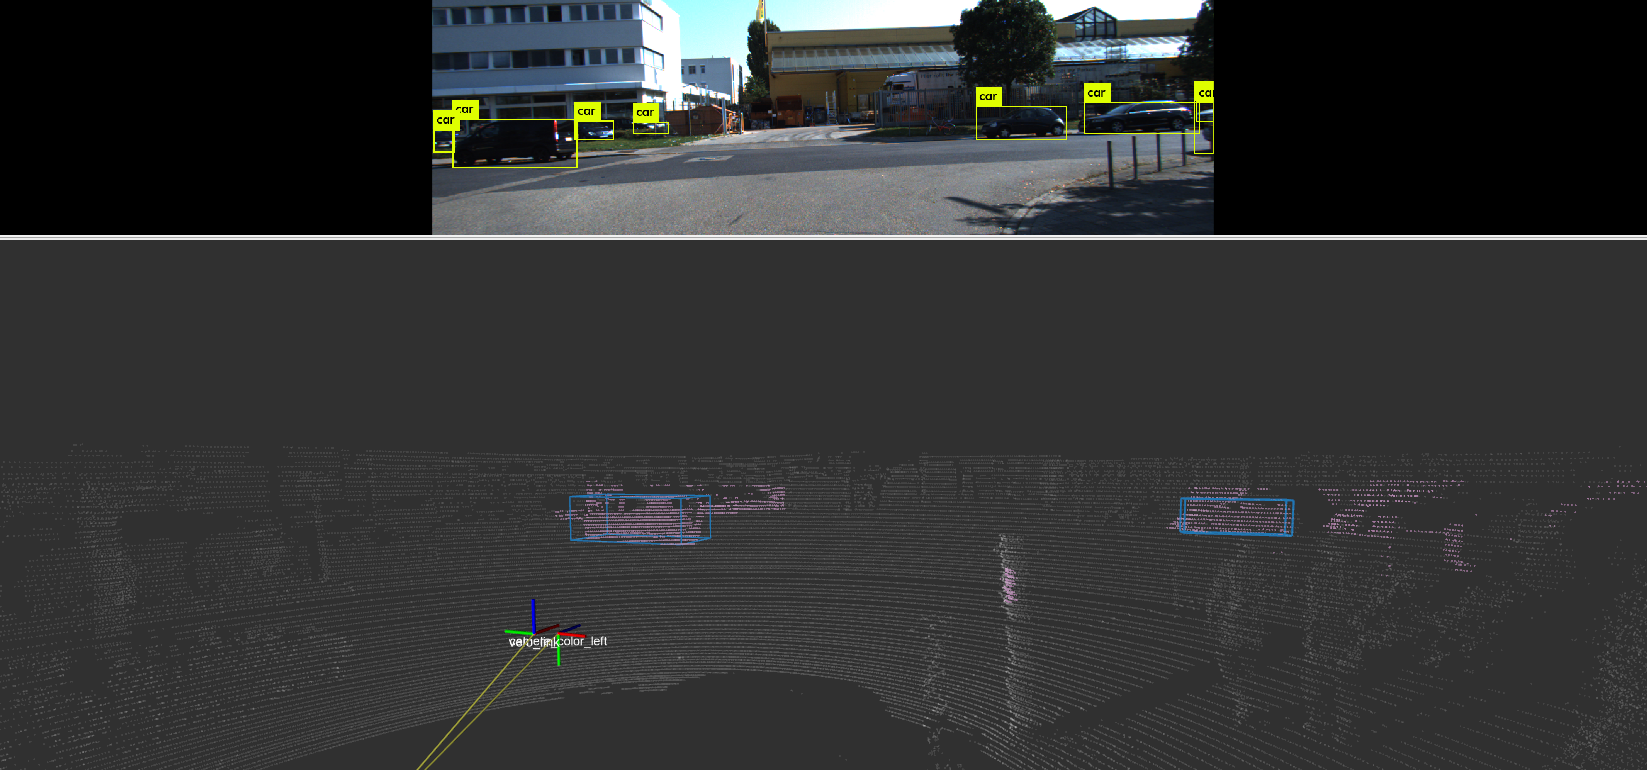
\includegraphics[width=\textwidth]{img/image-object-to-point-cloud/bboxes-side-view.png}
		\caption{In blue, two bounding boxes represented for the two closest cars, of all the \acp{roi} that were projected on the point cloud.}
		\label{fig:bboxes-3d-kitti-side}
	\end{subfigure}
	\\ \vspace{4mm}
	%\caption{Point Cloud tridimensional bounding boxes estimation using the methods described on Sub-Section~\ref{subsec:object-detection:bounding-boxes-and-roi}. The 3D bounding boxes are estimated from the image bounding boxes (top of sub-figure). The dark gray point cloud represents the original point cloud gathered by the \ac{lidar} and the lilac zones correspond to the filtered point cloud using \texttt{correspondences\_finder\_node}, node used to filter the original point cloud. In blue, the point cloud bounding boxes are shown, which are estimated from the image bounding boxes, given on the top of the sub-figures. Three different scenarios are presented: side~\subref{fig:bboxes-3d-kitti-side}, front~\subref{fig:bboxes-3d-kitti-front} and top~\subref{fig:bboxes-3d-kitti-top}. The original point cloud is presented using points 4 pixels wide and 10\% of transparency. The filtered point cloud is presented with points 6 pixels wide and 70\% of transparency. Bounding boxes line width is set to \SI{0.1}{\meter}.} 
	%\label{fig:bboxes-3d-kitti}
	\begin{subfigure}[c]{0.8\textwidth}
		\centering	
		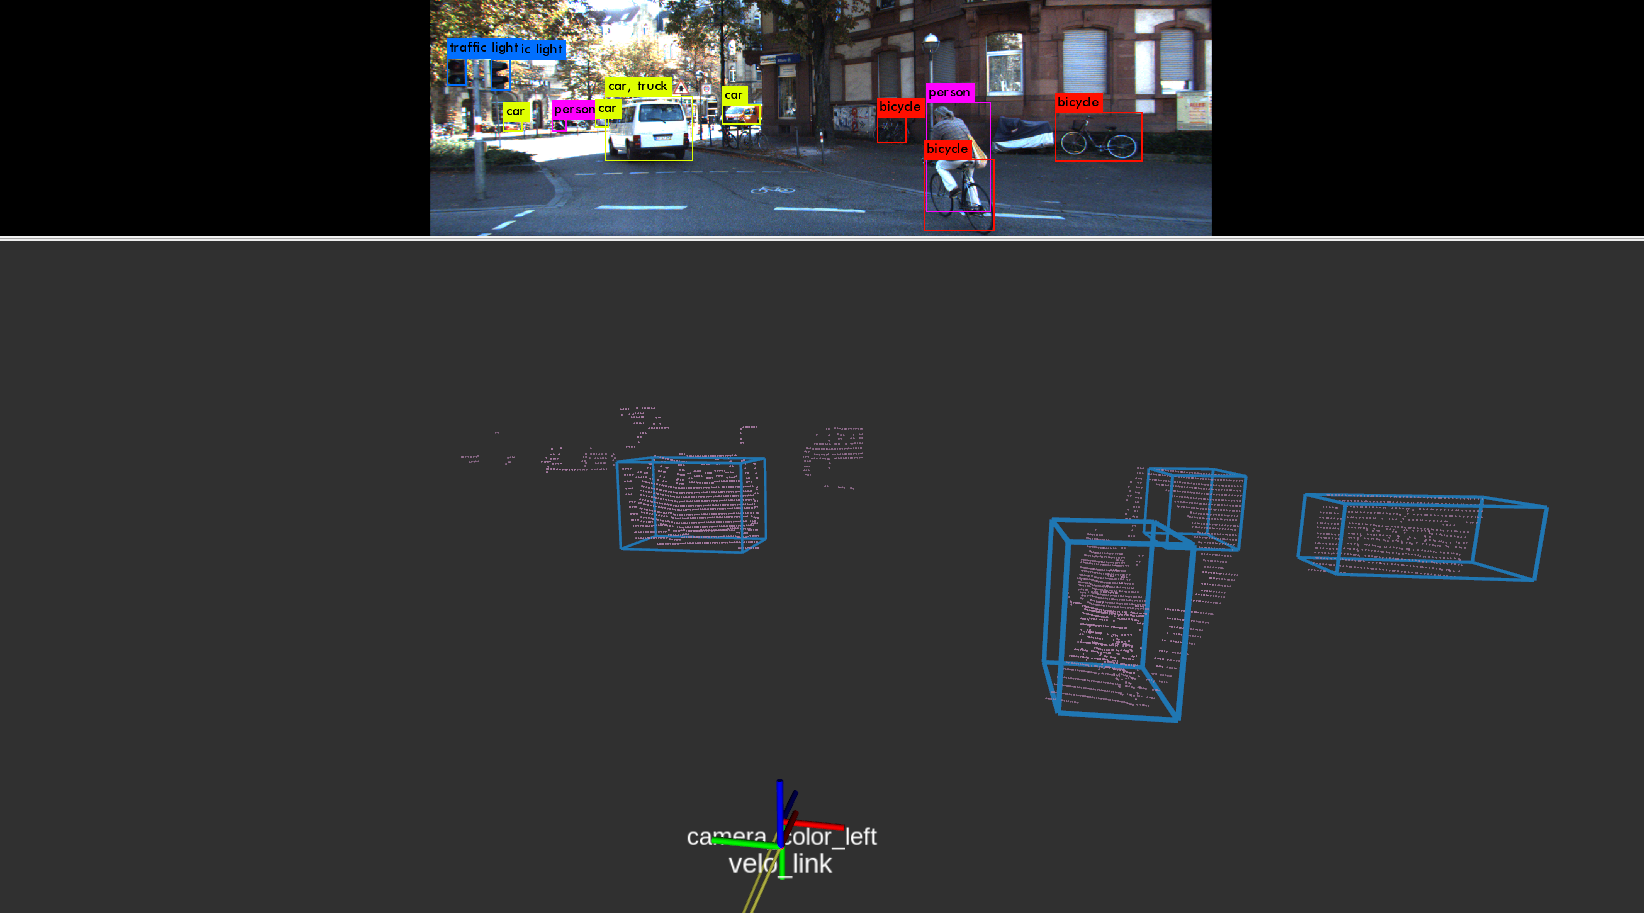
\includegraphics[width=\textwidth]{img/image-object-to-point-cloud/bboxes-front-view.png}
		\caption{On this sub-figure one can notice that not all the point cloud \acp{roi}' are within the bounding box.}
		\label{fig:bboxes-3d-kitti-front}
	\end{subfigure}
\end{figure}
% Continue the previous figure
\begin{figure}[!ht]\ContinuedFloat
	\centering
	%\\ \vspace{4mm}
	\begin{subfigure}[c]{0.8\textwidth}
		\centering
		\includegraphics[width=\textwidth]{img/image-object-to-point-cloud/bboxes-top-view.png}
		\caption{Two bounding boxes are presented in blue for the two closest cars, of all the \acp{roi} that were projected on the point cloud. The outliers of the \acp{roi} can also be seen, as several zones of the point cloud are filtered by the \texttt{correspondences\_finder\_node}.}
		\label{fig:bboxes-3d-kitti-top}
	\end{subfigure}
	\caption[Comparison between the estimated tridimensional bounding boxes' dimensions and position and the point cloud data, object clusters and \acs{roi}.]{Point Cloud tridimensional bounding boxes estimation using the methods described on Sub-Section~\ref{subsec:object-detection:bounding-boxes-and-roi}. The 3D bounding boxes are estimated from the image bounding boxes (top of sub-figure). The dark gray point cloud represents the original point cloud gathered by the \ac{lidar} and the lilac zones correspond to the filtered point cloud using \texttt{correspondences\_finder\_node}, node used to filter the original point cloud. In blue, the point cloud bounding boxes are shown, which are estimated from the image bounding boxes, given on the top of the sub-figures. Three different scenarios are presented: side~\subref{fig:bboxes-3d-kitti-side}, front~\subref{fig:bboxes-3d-kitti-front} and top~\subref{fig:bboxes-3d-kitti-top}. The original point cloud is presented using points 4 pixels wide and 10\% of transparency. The filtered point cloud is presented with points 6 pixels wide and 70\% of transparency. Bounding boxes line width is set to \SI{0.1}{\meter}.} 
	\label{fig:bboxes-3d-kitti}
\end{figure}


Despite the promising results, a caveat that is hard to notice is present on the implementation carried. The bounding boxes are of \acl{aabb} type, implying that they are oriented alongside the viewer coordinate frame. On our implementation, this frame is the \texttt{velo\_link}, the \ac{lidar} coordinate frame. Because the \ac{lidar} coordinate frame is not a fixed coordinate frame on the \ac{kitti} dataset, there are some situations where the requirement that the bounding boxes are aligned with the \ac{lidar} coordinate frame axis will force the bounding box to not be aligned with the road direction, specially when the \ac{kitti}'s car does a curve. Such behaviour will still result on a valid bounding box that encloses all the cluster, but its orientation will not coincide with the human perception of the ``correct'' object's bounding box. No attempts of solving this problem were carried. 

\section{Final Remarks}
On this chapter, image object detection is used to identify and crop \aclp{roi} on the point cloud. \ac{yolo} is the \acl{sota} \acl{cnn} selected to perform image object detection, which is integrated with the \ac{ros} network using \texttt{Darknet-ros} package. To determine the equivalent \ac{roi} on the point cloud from the image, two algorithms are developed. The first, establishes $2D \rightarrow 3D$ (from pixels to rays) correspondences and performs frustum filtering on the point cloud; and the second projects tridimensional point cloud points to the image plane, i.e., $3D \rightarrow 2D$ correspondences, selecting the points whose projection is contained on an image bounding box. Considering the accuracy of the \acp{roi} correspondences between image and point cloud, the latter algorithm is preferred, since errors were likely made during the implementation of the former; and the filtered point cloud is voxel filtered and clustered, using \ac{pcl}'s Voxel Grid and Euclidean Cluster filters. 

Such processing chain allows the identification of point cloud clusters that correspond to objects of interest, previously classified by the image object detection. This clusters can then be used for point cloud bounding box estimation and \ac{lidar} interference analysis on objects of interest. Regarding the bounding box estimation, two types are researched: \acf{obb} and \acf{aabb}. Since the goal of bounding box drawing is to show the viewer the objects of interest and their limits, \ac{aabb} are preferred and more intuitive. To speed up the \ac{pcl}'s native implementation of \ac{aabb} computation, the \ac{aabb} position, orientation and dimensions are computed using an alternative method implemented by us, based on \texttt{pcl::getMinMax3D} and high school Euclidean geometry, which yield the similar results and require less than 5\% of the previous execution time.

From this chapter, the main outcome is a processing chain that is capable of extracting the point cloud subsets, representing objects of interest, previously detected on image using image object detection. Such processing chain is relevant to the topic of \ac{lidar} interference since it allows us to analyze the \ac{lidar} interference on objects that are relevant for self-driving vehicles, such as cars, cyclist and pedestrians. The requirements of such implementation are that the camera's and \ac{lidar}'s must be intrinsic calibrated and that their extrinsic calibration must be known.


\chapter{\acs{lidar} Interference}
\label{chapter:lidar-interference}

\ac{lidar} interference occurs when the signal of one \ac{lidar}, ``A'', interferes with the signal of another \ac{lidar}, ``B'', affecting its measurements, i.e., \ac{lidar}'s ``B'' capability to measure the distance is not independent of the presence of another \ac{lidar} on its surroundings. In telecommunications, when two devices on the same channel or physical environment interact, creating an undesirable effect with negative consequences, we are in the presence of crosstalk. In a \ac{lidar} interference scenario, this interference can be direct or indirect (the beam is reflected on other surface(s) before hitting \ac{lidar} ``B'') and is a crosstalk phenomenon between the two \acp{lidar}.

The main goal of this thesis is to study the \ac{lidar}'s interference behaviour, expanding the previous work, presented in Section~\ref{sec:sota:lidar-interference}. \acl{sota} in \ac{lidar} interference is still reduced, with the major contributions from only two research teams (Gunzung Kim\etal~\cite{Kim2015c, Kim2017} and Gerald Popko\etal~\cite{Popko2019a, Popko2019b}), both using only two-dimensional \acp{lidar}, i.e., rotating \acp{lidar} that can scan a single line of the scene.

On this chapter, we start by explaining the additions to the previously described experimental setup, on Section~\ref{sec:calibration:experimental-setup}, that allows us to investigate the impact of several parameters on \ac{lidar} interference behaviour. Test scenarios are detailed and the test conditions under which data was acquired are explained. Since one of the thesis objectives, detailed in Section~\ref{sec:introduction:objectives}, is to create a comprehensive experimental dataset with different metrics for future tests on \ac{lidar} interference, we describe how the experimental dataset was organized to ensure it could be easily reused and also to streamline data analysis in this study.

Our first \ac{lidar} interference analysis results are obtained from Bosch\cp~datasets, allowing a qualitative assessment of the interference. Based on these results, we sought to explain this behaviour by quantifying the number of outliers that have no physical context on the data, such as points below ground or outside a closed room dimensions.

To provide a more in-depth analysis of the interference, a comparison with a ground-truth model of the test environment is required. We propose two methods to generate such ground truth model from the data without interference. Using these models, we also propose two methods to measure the interference, unveiling their algorithms and results.

Following up on the outcomes provided by Chapter~\ref{chapter:object-detection}, we apply the previous algorithms onto the selected \acp{roi} on the point cloud, that correspond to the bounding boxes of image objects previously detected on the image, using the calibration notions gathered from Chapter~\ref{chapter:calibration}.

Lastly, we conclude our findings and compare them with the current \acl{sota} on \ac{lidar} interference.

%%%%%%%%%%%%%%%%%%%%%%%%%%%%%%%%%%%%%%%%%%%%%%%%%%%%%%%%%%%%%%%%%%%%%%%%%%%%%%%%%%%%%%%%%%%%%%%%%
%%%%%%%%%%%%%%%%%%%%%%%%%%%%%%%%%%% EXPERIMENTAL SETUP %%%%%%%%%%%%%%%%%%%%%%%%%%%%%%%%%%%%%%%%%%
%%%%%%%%%%%%%%%%%%%%%%%%%%%%%%%%%%%%%%%%%%%%%%%%%%%%%%%%%%%%%%%%%%%%%%%%%%%%%%%%%%%%%%%%%%%%%%%%%


\section{Experimental Setup}
\label{sec:lidar-interference:experimental-setup}

Expanding the previous experimental setup, detailed in Section~\ref{sec:calibration:experimental-setup}, requires adding another \ac{lidar} for acting as an interferer. This \ac{lidar} is mounted on a tripod and serves the purpose of interfering with the measurements of the first \ac{lidar}, already present on the earlier version of the experimental setup (see Figure~\ref{fig:experimental-setup}), which becomes its ``victim''\footnote{The terms victim and interferer, when referring to \ac{lidar} interference, are first connoted by Gunzung Kim\etal on~\cite{Kim2015a, Kim2015b, Kim2015c, Kim2017}, and later adopted by Gerald Popko\etal~\cite{Popko2019a, Popko2019b}. To keep the notation coherent with the \acl{sota}, we will use the same denominations on this chapter.}.

The interferer \ac{lidar} is a HESAI\cp~Pandar40\texttrademark, a 40 beams \ac{tof} rotating \ac{lidar} that operates at a wavelength of \SI{905}{\nano\meter}. Pandar40 supports various measurement modes based on the return pulse (Strongest, Last, Dual) and can be connected to a \ac{gps} receiver for geopositioning and synchronization with an external clock. It also supports two rotation velocities: 600 or 1200 \ac{rpm}, which result in different angular steps and point cloud refresh rate. 

Pandar40's \ac{lidar} has an asymmetrical vertical \ac{fov}, varying from \SIrange{-16}{+7}{\degree}. A larger channel density occurs between the angles \SI{-6}{\degree} and \SI{+2}{\degree}, with 25 pairs of lasers and photodetectors with \SI{0.33}{\degree} apart from each other. From \SIrange{-16}{-6}{\degree} and \SIrange{+2}{+7}{\degree}, the angular step between the pairs of lasers and photodetectors is \SI{1}{\degree}, and only 15 pairs of lasers and photodetectors are used: 5 above and 10 below.

The full specifications of the HESAI Pandar40 can be accessed on~\cite{Pandar40UserGuide} and the relevant specifications for this work are summarized on Table~\ref{tab:pandar40-specs}.

\begin{table}[H]
\centering
\renewcommand{\arraystretch}{1.2}
\rowcolors{3}{gray!10}{white}
\begin{tabular}{@{}p{6cm}c@{}}
	\toprule
	Specifications & Value \\
	\midrule
	Wavelength & \SI{905}{\nano\meter} \\
	Motor \ac{rpm} & 600 \\
	Angular Step & \SI{0.2}{\degree} \\
	Vertical \ac{fov} & \SI{23}{\degree} \\
	Horizontal \ac{fov} & \SI{360}{\degree} \\
	Maximum Scanning Distance & \SI{200}{\meter} @20\% reflectivity \\
																				 & $\pm \SI{5}{\centi\meter}$, from \SIrange{0.3}{0.5}{\meter} \\
	\rowcolor{white} \multirow{-2}{*}{Measurement Accuracy} & $\pm \SI{2}{\centi\meter}$, from \SIrange{0.5}{200}{\meter} \\
	\bottomrule
\end{tabular}
\caption[HESAI Pandar40 relevant specifications.]{HESAI Pandar40 relevant specifications. Source~\cite{Pandar40UserGuide}.}
\label{tab:pandar40-specs}
\end{table}

The tripod used for the experimental setup is a Velbon\cp~CX-460\texttrademark~tripod, that also has a central monopod. For increased stability on the measurement procedure, the monopod was never used. The tripod ranges in height from approximately \SIrange{0.62}{1.28}{\meter}, measured from its feet to its basis. Since the tripod used is a camera tripod, a gimmick must be done to ensure proper fixation of the Pandar40 \ac{lidar}, by replacing the universal camera support bolt with an \SI{12}{\milli\meter} length M6 bolt, tightened with an M6 nut and two metal rings. The Pandar40, secured on the tripod is shown in Figure~\ref{fig:pandar40-on-tripod}.

\begin{figure}[H]
\centering
\includegraphics[width=0.4\textwidth]{img/experimental-setup/pandar40-on-tripod.jpg}
\caption[HESAI Pandar40 \ac{lidar} on a Velbon CX-460 tripod.]{HESAI Pandar40 \ac{lidar} on a Velbon CX-460 tripod.}
\label{fig:pandar40-on-tripod}
\end{figure}

Despite the two \acp{lidar}'s laser nominal wavelengths being slightly difference, no majors drawbacks are expected due to the mismatch, due to wavelength shift caused by the operating temperature and that the \ac{ir} filter used as a bandwidth of, at least, \SI{10}{\nano\meter}. Velodyne's VLP-16, the victim, operates at \SI{903}{\nano\meter} and HESAI Pandar40, the interferer, operates at \SI{905}{\nano\meter}. Ideally, the same \ac{lidar} model would be used for the victim and interferer, but such material was not available. Nevertheless, we are unable to easily predict how the different number of channels, asymmetric channel distribution, variable angular step and different laser wavelength will impact the interference behaviour, due to the lacking of prior knowledge available on the area. Such study is out of the focus of this study and is left for future work.

\subsection{Experimental Test Scenarios}
\label{subsec:lidar-interference:test-scenarios}

Two locations were used as test scenarios for \ac{lidar} interference: Aveiro's \ac{it} Dark Room and \ac{irislab} \ac{msl} robotic soccer field. At the former, acquaintance with the experimental setup, calibration procedures and tests to gathered preliminary knowledge on \ac{lidar} interference were carried. At the latter, experimental tests were devised to assess the impact of relevant parameters under study on \ac{lidar} interference. 

Aveiro's \ac{it} Dark Room is an optical laboratory that is capable of blocking all external light (hence its name). It measures $\SI{5.20}{\meter} \times \SI{6.97}{\meter} \times \SI{2.80}{\meter}$ and is equipped with benchtop, chairs, optical experimental setup, among other things, creating a rich scenario for a \ac{lidar} rangefinder. 
\ac{irislab} \ac{msl} robotic soccer field measures $\SI{18.0}{\meter} \times \SI{11.5}{\meter}$ and is placed inside \ac{irislab} building, a research facility whose main division has $\SI{34.346}{\meter} \times \SI{16.097}{\meter} \times \SI{4.289}{\meter}$, if measured to the ceiling and not the ceiling girders. 

All distance measures presented on this Chapter are taken using a LOMVUM LV66V \SI{80}{\meter} handheld laser rangefinder, which is used in this context as the distance calibration instrument. When taking measures, the orientation of the rangefinder was kept in the interval of $[\SI{-0.2}{\degree}, \SI{0.3}{\degree}]$. The error associated to each laser measurement, according to LOMVUM datasheet\footnote{No online manual was found. Measurement error determined by consulting the product printed datasheet, supplied with the device.} is \SI{1.5}{\milli\meter}. To minimize the error introduced by the human operator, 10 measurements were done and their average was taken using the LOMVUM's laser rangefinder capabilities.


\subsection{Parameters under study}
\label{subsec:lidar-interference:parameters-under-test}
On \ac{irislab}, several tests were devised to tackle the problem of \ac{lidar} interference from different perspectives. Test scenarios were carried, where only one parameter is varied, in an attempt to understand the interference behaviour between data. The test parameters under study, from which different datasets were recorded are:

\begin{itemize}
	\item \textbf{Distance between \acp{lidar}:} Keeping the \acp{lidar} azimuthal origin aligned and with their optical axis at the same height, the distance between the interferer and victim is changed, by moving the interferer further away. The distance between the two was varied in steps of \SI{1}{\meter}, from \SIrange{1}{12}{\meter};
\item \textbf{Height:} To evaluate the impact of the elevation angle, for a fixed distance between the two \acp{lidar}, with its azimuthal origin aligned, the height between the two is varied in non-uniform steps, from \SIrange{0.623}{1.277}{\meter} measured in relation to the floor, which results in \SIrange{-0.295}{0.359}{\meter} when compared with the victim \ac{lidar} height;
\item \textbf{\acp{lidar} \ac{los} obstruction:} To quantify the impact of direct and indirect interference, an obstacle is placed on the \acp{lidar} \ac{fov}, breaking the \ac{los} between the two \acp{lidar}. This test scenario is similar to that of the Distance tests, but places the obstacle at the middle distance between the victim and interferer \ac{lidar}. The measurements were carried out only when the distance between the interferer and the \ac{lidar} was an even number.
\item \textbf{Rotation Speed:} To measure the impact of different rotation speeds between the \acp{lidar}, the victim's \ac{lidar} is kept at the same rotation speed as the other tests, while the interferer \ac{lidar} rotation speed is changed. Distance is constant, the \ac{lidar}'s azimuthal origin is aligned and their optical axis is at the same height;
\item \textbf{Orientation:} To study the interference directionality, the relative angular position between the victim's and the interferer \ac{lidar} is changed, while keeping their optical axis at the same height and the same distance for all variations of this parameter.
\end{itemize}


\subsection{Dataset Organization}
A thesis objective on its own (see Section~\ref{sec:introduction:objectives}), dataset organization is a crucial for a proper data analysis. With 5 parameters under test, each with several values, 60 different interference test exists, in addition to camera calibration data and data without interference. In total, more than \SI{600}{\giga\byte} of pre-processed raw data, ready to be analyzed, is stored, in a total of almost 180 \ac{ros} bag files, totalling almost 4 hours and 20 minutes of playable data. Several hundred files, among camera calibration, rigid body transformation and results, are also contained in the dataset structure, for a total of more than \SI{1}{\tera\byte} of data and results.

A comprehensive diagram that details the dataset directory and file tree hierarchy for data recording is given on~\nameref{appendix:datasets-tree}. The \textit{Experimental Datasets} folder is the root folder of the data, containing the two test locations, \textit{IRIS Laboratory} and \textit{IT2 Dark Room}. 

The standardization of test scenarios started at \ac{it} 2 Dark Room, but only matured at \ac{irislab}. This standardization forces guidelines on file and folder naming, directory structure organization and data to record. On every folder, a \textit{README.md} file is present, detailing the files and/or folders in its hierarchy level, and the test conditions, if applicable. 

At \ac{it} 2 Dark Room, only \textit{Scenario B} follows these guidelines, which were inspired by \ac{kitti}'s dataset~\cite{Geiger2013a}. Since our setups location is fixed, each location defines a root folder for all the tests happening in that location, with its subfolders being the day on which the data was acquired. These type of folders contain  3 subfolders, whose goal is detailed below and an extract of its  hierarchy organization is given on Figure~\ref{fig:test-subfolders}.

\begin{figure}[H]
\centering
\includegraphics[scale=0.3]{img/datasets/test-subfolders.png}
\caption[Dataset folder hierarchy for a ``test day''.]{Detail of the hierarchy of a ``test day''. On each day data was recorded, calibration and ground-truth data were recorded. \textit{Multiple Lidar Interference} folder contains the parameters under test and each of the tested values.}
\label{fig:test-subfolders}
\end{figure}


\begin{enumerate}
\item \textit{Camera Calibration}: Contains the calibration images, intrinsic calibration parameters, \ac{ros} bag files containing the camera and \ac{lidar} raw and pre-processed data and the log file of the calibration procedure;
\item \textit{Ground Truth}: One or more \ac{ros} bag file containing the static scenario, without objects of interest placed on the camera and \ac{lidar}'s \ac{fov} and without \ac{lidar} interference;
\item \textit{Multiple LiDAR Interference}: This folder contains a series of subfolders, each for a parameter under test. For each parameter under test folder, subfolders contain the data and results for each of the value that the parameters takes.
\end{enumerate}

On a specific value for a parameter under test, three bag files are present, as shown in Figure~\ref{fig:parameter-test-files}. \textit{interference.bag} is a pre-processed \ac{ros} bag file that contains only \ac{lidar} data with interference. This pre-processing consists on cropping the \textit{original\_raw.bag} file to remove the initial seconds (from \SIrange{20}{30}{\second}), when the interferer \ac{lidar} is still booting up. \textit{ground\_truth} corresponds to data recorded under the conditions of \textit{interference.bag}, but without interference, i.e., the interferer \ac{lidar} is at its position for the test, but switched off.

\begin{figure}[H]
\centering
\includegraphics[scale=0.3]{img/datasets/parameter-test-files.png}
\caption[Dataset file hierarchy for a single value of a parameter under test.]{Data recorded using \texttt{rosbag} tool, for a single value of a parameter under test. \textit{README.md}, on this type of folder, details the conditions under which data was gathered.}
\label{fig:parameter-test-files}
\end{figure}


In \textit{IRIS Laboratory} folder, two test folders are present, containing all the data gathered on \ac{irislab}, \textit{2019-08-28} and \textit{2019-08-29}. For each of the folders, different calibration parameters are available, along with ground truths and calibration data. For \textit{\ac{it} 2 Dark Room}, only the data on the folder \textit{2019-07-31} is relevant to interference analysis.

To ease the access to this data structure, \texttt{datasets\_path} library was implemented, both on C++ and Python 3, to allow ubiquitous managing of data loading for tests and saving of results.


%%%%%%%%%%%%%%%%%%%%%%%%%%%%%%%%%%%%%%%%%%%%%%%%%%%%%%%%%%%%%%%%%%%%%%%%%%%%%%%%%%%%%%%%%%%%%%%%%
%%%%%%%%%%%%%%%%%%%%%%%%%%%%%%%%%%%%% BOSCH DATASET %%%%%%%%%%%%%%%%%%%%%%%%%%%%%%%%%%%%%%%%%%%%%
%%%%%%%%%%%%%%%%%%%%%%%%%%%%%%%%%%%%%%%%%%%%%%%%%%%%%%%%%%%%%%%%%%%%%%%%%%%%%%%%%%%%%%%%%%%%%%%%%


\section{Bosch\cp~Dataset}
We start by investigating \ac{lidar} interference using a dataset provided by Bosch. This dataset consists of 3 \ac{ros} bag files, one recorded by a HESAI Pandar40 and two other by Velodyne's VLP-16. Each of the bag files correspond to the same experimental scenario: the two \acp{lidar} are placed, side by side, on top of a table, with the Pandar40 about \SI{50}{\centi\meter} to the left of the VLP-16. For each of the tests, data is recorded for about \SIrange{10}{15}{\second} and the two \acp{lidar} are always switched on.

To analyze the interference, we start by analyze at the data in \texttt{Rviz}, noticing two phenomena: 

\begin{enumerate}
\item Data appears to be more noisy, as if it was oscillating with greater magnitude around a fixed point on its measurement axis, when comparing with \ac{kitti}'s dataset;
\item Some measurements correspond to points outside of the room dimensions.
\end{enumerate}

For the first case, we present two hypotheses: it is caused by the interference of the other \ac{lidar}, or due to the measurements being taken in small rooms. To understand the second phenomenon, a two-dimensional scatter map of the point cloud, viewed from above, is plotted. This representation does not take in consideration the measurement density, which might be misleading, since interfered measurements should have a higher ``geometric'' dispersion and a lower point density when comparing with the correct measurements of the real world.

These results are present on Figure~\ref{fig:bosch-pandar-vs-vlp16}, with the left sub-figure, (\subref{fig:bosch-pandar40}), showing HESAI's Pandar40 data, represented in green, and the right sub-figure, (\subref{fig:bosch-vlp16-1}), showing Velodyne's VLP-16 data, represented in yellow. For each of the sub-figures, we notice in the center a rectangular shape, the room, and the outliers are distributed in a circular arrangement, with preference for some azimuthal angles. The circular range is due to the hardware time window to measure the reception pulse and software distance threshold to register the data. On Pandar40, the software constrain is \SI{200}{\meter} and on VLP-16 is \SI{130}{\meter}. 

Considering the HESAI's \ac{lidar} is left to the Velodyne's \ac{lidar}, the occurrence of interference seem to be more significant to HESAI's right, i.e., between the two \acp{lidar}. On the other hand, Velodyne's outliers tend to its left, the side on which the HESAI's is in. With HESAI's outliers concentrated on its first geometric quadrant and Velodyne's outliers on the second geometric quadrant, such results seem to indicate that interference is directional. However, from this data we cannot determine if this is due to direct interference, reflections or both.

\begin{figure}[ht!]
\centering
\begin{subfigure}[t]{0.45\textwidth}
	\includegraphics[width=\textwidth]{img/bosch/pandar40.png}
	\caption{HESAI's Pandar40 data scatter plot.}
	\label{fig:bosch-pandar40}
\end{subfigure}
\qquad
\begin{subfigure}[t]{0.45\textwidth}
	\includegraphics[width=\textwidth]{img/bosch/vlp16-test1.png}
	\caption{Velodyne's VLP-16 data scatter plot}
	\label{fig:bosch-vlp16-1}
\end{subfigure}
\caption[Scatter plot top-view of both \acp{lidar} interference on the dataset provided by Bosch.]{Scatter plot of the data gathered by HESAI's Pandar40, (\subref{fig:bosch-pandar40}), and Velodyne's VLP-16, (\subref{fig:bosch-vlp16-1}). The measurements are plotted only on the X-Y plane, flattening the height of the points.}
\label{fig:bosch-pandar-vs-vlp16}
\end{figure}

We also analyze the results from the second VLP-16 bag file, and compare with the first, on Figure~\ref{fig:bosch-vlp16-comparison}. The previous shown data, on Figure~\ref{fig:bosch-vlp16-1} is shown in yellow and the second dataset in blue. In the center, the room can be seen, and the data, independently of the bag file, seems to have the same dispersion and directionality.

\begin{figure}[ht!]
\centering
\includegraphics[scale=0.33]{img/bosch/vlp16-tests-overlaid.png}
\caption[Scattered plot of VLP-16 interference taken on two different instants, on the same conditions.]{Scatter plot of the \ac{ros} bags containing Velodyne's VLP-16 data, gathered under the same conditions with almost an hour of difference. Thee measurements are plotted only on the X-Y plane, flattening the height of the points. Comparison between the grid and blue points shows a macro-correspondence.}
\label{fig:bosch-vlp16-comparison}
\end{figure}

Originally, this dataset were not aimed for a detailed analysis on \ac{lidar} interference neither for our approach to study the interference. The sole purpose of such dataset was to illustrate the phenomena of interference. Since the scenario was not static and no data without interference is present, this dataset cannot be used for a refined analysis of the interference, due to the approach and methods we devise suppose that the environment is static, in order for a ground truth model to be generated. Also, no camera is present and therefore, no object detection processing chain can be implemented (similar to Chapter~\ref{chapter:object-detection}). 

Our solution is then to acquire datasets on the conditions described on Section~\ref{sec:lidar-interference:experimental-setup}. For Bosch dataset, we quantize these outliers and try to understand more about their behavior, which is the approach detailed on the next Section.


%%%%%%%%%%%%%%%%%%%%%%%%%%%%%%%%%%%%%%%%%%%%%%%%%%%%%%%%%%%%%%%%%%%%%%%%%%%%%%%%%%%%%%%%%%%%%%%%%
%%%%%%%%%%%%%%%%%%%%%%%%%%%%%%%%%% ROOM OUTLIERS ACCOUNTING %%%%%%%%%%%%%%%%%%%%%%%%%%%%%%%%%%%%%
%%%%%%%%%%%%%%%%%%%%%%%%%%%%%%%%%%%%%%%%%%%%%%%%%%%%%%%%%%%%%%%%%%%%%%%%%%%%%%%%%%%%%%%%%%%%%%%%%


\section{Room Outliers Accounting}
\label{sec:lidar-interference:room-outliers}
After the qualitative analysis of the previous Section on Bosch's dataset, from which we concluded that the \ac{lidar} interference appears to be directional and causes outliers outside of the room dimensions, this Section details the implementation and results of a quantitative approach to analyze the events described on phenomenon 2: \ac{lidar} measurements outside room dimensions.

To analyze the data, a \ac{ros} node, with both offline and online versions, was implemented. Offline operation implies that the node does not have real-time constraints, being capable of handling large \ac{ros} bag files and datasets. The main difference from the online operation, that has been used so far, is that the node does not require another node on the network to publish data for it (typically, a \ac{ros} bag player or a device driver) and the \ac{ros} network does not need to be setup up and running. Instead, the node loads and parses the bag file, as fast as it can or as fast as it is instructed to, keeping its data private on its own program memory. This alternative permits processing large amounts of data and realizing complex analysis on it.

To quantify this interference, the node only needs to know the room dimensions, which we considered to be the majorant and minorant of the room dimensions along each of the 3 Cartesian axes. With it, it can determine the number of point cloud messages received, average number of points per message, absolute and relative number of outliers and inliers. To account for some noise on the data, to the room limits dimensions, a 5\% tolerance is applied. 

An outlier is a point that is not contained within the room dimensions (approximated as a parallelepiped), in all three Cartesian coordinates, considering also the tolerance scaling. Given a point under classification, $P$, and a tolerance, $t$, Equation~\eqref{eq:box-outlier-condition} describes the mathematical decision applied to determine if that point cloud point is an inlier or an outlier.

\begin{equation}
\label{eq:box-outlier-condition}
\begin{cases}
	\begin{aligned}
		\text{inlier}, \qquad \text{if\ } P \in & [\min(x) \cdot t, \max(x) \cdot t] \cup [\min(y) \cdot t, \max(y) \cdot t]  \\
																					&					 \cup [\min(z) \cdot t, \max(z) \cdot t] 
	\end{aligned} \\
	\text{outlier}, \qquad \text{otherwise}
\end{cases}
\end{equation}

Despite this analysis not accounting for the possible interference inside the room dimensions, this interference model intends to measure what, to the ``naked eye'', is clearly an erroneous measure, caused by \ac{lidar} interference: measurements outside the physical dimensions of the room where the \acp{lidar} are located. Since the possible interference inside the room dimensions is not considered, we can view this metric as a minorant for the \ac{lidar} interference.


\subsection{Bosch Dataset}
\label{subsec:lidar-interference:room-outliers-bosch}
To determine the room dimensions in Bosch dataset, we display the data on \texttt{RViz} and then use the selection tool to determine the maximum and minimum value on each axis that defines the room dimensions. This process is manual, and prone to error, specially since on this dataset, the \ac{lidar} axes are not oriented with the room\footnote{We can say that the \ac{lidar} axes are oriented with the room when a straight wall has one of its coordinates fixed on the \ac{lidar} coordinate frame, i.e., for every wall, there a \ac{lidar} axis that is parallel with the normal defined by the plane of the wall.} After determining such parameters, the data is analyzed and the results are presented in Table~\ref{tab:bosch-dataset-stats}.

\begin{table}[!ht]
\centering
\renewcommand{\arraystretch}{1.2}
\begin{tabular}{@{}llC{2cm}C{2.5cm}C{3.5cm}@{}}
	\toprule
	\multicolumn{2}{l}{Test Scenario} & \# \ac{lidar} messages & Average Points Per Message &  Normalized number of interferer points \\
		\midrule
	\multicolumn{2}{l}{\textit{Velodyne VLP-16}} & & & \\ 
	\phantom{ab} & \SI{5}{\hertz}  & 80  & 45582.3 & $1.10\E^{-3}$ \\ 
							 & \SI{10}{\hertz} & 199 & 22849.8 & $1.44\E^{-3}$ \\ 
	\midrule
	\multicolumn{2}{l}{\textit{HESAI Pandar40}} & & &  \\ 
	\phantom{ab} & \SI{20}{\hertz} & 406 & 25642.5 & $2.14\E^{-3}$ \\
	\bottomrule
\end{tabular}
\caption[Room outlier analysis on Bosch interference dataset.]{Statistics of Bosch interference dataset. Room dimensions were manually determined from the interference dataset by selecting the points that correspond to the maximum and minimum value alongside the axis.}
\label{tab:bosch-dataset-stats}
\end{table}

On Bosch's experimental setup, we can conclude that between 1 and 2 outliers outside of the room limits are expected for every 1000 points of data. These results offer a first glimpse of \ac{lidar} interference, but we must restrain ourselves from premature conclusions.

Pandar40 seems to have a higher presence of outliers than VLP-16, and data seems to suggest that a higher rotation speed increases the occurrence of ``outside of the room dimensions'' outliers. However, the data diversity is reduced and the data that is available has low statistically significance, since the number of tests is small and the duration of each bag file is shorter than \SI{20}{\second}.

We also need to consider that the room limits were manually determined, therefore these results are more prone to be affected by human error, which may be causing \ac{lidar} measurements inside of the room dimensions, inliers, to be considered erroneous and marked as outliers. Since the \ac{lidar} axes were also not oriented with the room\footnote{A rotation to align the point cloud with the room could have been applied to the dataset, which could have improved the determination of the room dimensions. However, since there was little information regarding the test conditions, we opt not to, to prevent biasing the dataset.}, the errors are more likely. 

The distance between the two \acp{lidar} is \SI{0.5}{\meter}, less than 0.5\% of their measurement range. They are on top of a table, which causes, at that distance, the lower beams of one \ac{lidar} to be reflected onto the other \ac{lidar}, increasing mutual interference.

Despite no conclusive verdicts can be extracted from this data, we can affirm that the conditions under which this dataset is taken fosters the occurrence of mutual \ac{lidar} interference, biasing the data by creating laboratorial scenarios not observed in realistic settings. We cannot be sure whether the higher number of interference on the HESAI Pandar40 is because it has more lasers or because additional measures have been implemented on Velodyne VLP-16 to mitigate mutual interference\footnote{Velodyne as been working on this topic. See the Release Notes on~\cite{vlp16}.}. 

\subsection{Our Experimental Dataset}
\label{subsec:lidar-interference:room-outliers-experimental-setup}
For our experimental dataset, we can automate the determination of the room dimensions from the data, since we have measurements of the test environments without interference. Therefore, the previous uncertainties regarding the manual determination of room limits are no longer present. To automate the process, we developed a \ac{ros} node that parses a ground truth bag file and determines the room dimensions, considering the minorant and majorant points of the point cloud, on the \ac{lidar} coordinate frame. 

As stated in Sub-Section~\ref{subsec:lidar-interference:parameters-under-test}, 5 parameters under test are varied on our dataset, on \ac{irislab} facilities. The data gathered is analyzed and the results, for each of the parameters, are presented below, with the exception of the rotation speed.

Changing the rotation speed would require accessing HESAI's Pandar40 web-server, through an Ethernet connection, to configure its rotation speed~\cite{Pandar40UserGuide}. These attempts, however, were unfruitful, despite the several \ac{ros} drivers used, including official \ac{sdk} from HESAI\cp. Alternatively, VLP-16 rotation speed could be changed, instead, but we wanted the victim operation parameters to be constant at all time. Therefore, we opt to abandon the acquisition of interference data when the two \acp{lidar} operate at a different rotation speed.

\subsubsection{Distance}
The distance parameter was varied from \SIrange{1}{12}{\meter}, with steps of \SI{1}{\meter}. While varying the interferer position, the victim's \ac{lidar} remains unchanged, and the interferer height is kept constant to ensure that the \ac{lidar}'s optical center is at approximately the same height, with their relative orientation kept at approximately \SI{0}{\degree}.

The normalized number of outliers, regarding the number of received points, is visualized on the bar chart on Figure~\ref{fig:box-filter-outliers-distance}, for all the distances. The range of outliers varies from $10^{-7}$ to $10^{-5}$, significantly different from the results on Bosch's dataset, which were all on the order of magnitude of $10^{-3}$. Comparing with Bosch scene, \ac{irislab} is an open space larger than the room where Bosch dataset was captured. Due to the difference in magnitude between the two results, we can affirm that the proximity of the \acp{lidar} among themselves and walls increase the interference. 

\begin{figure}[!ht]
\centering
\includegraphics[width=0.8\textwidth]{img/lidar-interference/box-filtering/interference-box-filter-outliers-distance.png}
\caption[Relative number of outliers when the distance between the \acp{lidar} is varied on \ac{irislab}.]{Ratio between the number of outliers with respect to the total number of detected points accounting when the parameter under test is the distance between the two \acp{lidar}. The outlier accounting method is detailed on Equation~\eqref{eq:box-outlier-condition}.}
\label{fig:box-filter-outliers-distance}
\end{figure}

Despite the data not revealing any perceivable patterns, there is a tendency for the higher values of outliers to occur for a closer distance between the \acp{lidar}. Note that these results do not indicate that the interference is higher the shorter the distance, but that the interference causes a higher number of points to be outside of the room dimensions if the two \acp{lidar} are closer. 

\subsubsection{Height}
Due to the \ac{lidar} photodetectors and lasers orientation and internal organization, there are, theoretically, relative positioning and orientation between the two \acp{lidar} that either minimize the interference or potentiate it. No theoretical analysis of such relations was carried, due to its impracticality: the application of such results to an extent it would benefit this research, i.e., gathering data under positions of maximum and minimum interference, would require the alignment of a laser and a photodetector, whose position is only approximately known, in free space of two different rotating devices. To precisely known the distance and relative position of the optical components would require disassembling the \ac{lidar}, which is not an option.

For a fixed distance, our goal was to understand if variations of several orders of magnitude occurred when the relative height between the devices changed, which could hint on the relevance of the relative positioning between the \acp{lidar} and its impact on the \ac{lidar} interference behaviour.

Figure~\ref{fig:box-filter-outliers-height} shows our analyzes of this parameter by measuring the relative number of outliers outside the room dimensions. Height difference values, presented on the x-axis of the bar chart, indicate the relative height between the HESAI and the Velodyne \acp{lidar}. The interferer \ac{lidar} was placed at a distance of \SI{4}{\meter} of the victim and their relative orientation was kept approximately at \SI{0}{\degree}.

\begin{figure}[!ht]
\centering
\includegraphics[width=0.8\textwidth]{img/lidar-interference/box-filtering/interference-box-filter-outliers-height.png}
\caption[Relative number of outliers when the height between the \acp{lidar} is varied on \ac{irislab}.]{Outliers analyzes when the parameter under test is height. On the x-axis, the height variation indicates the Pandar40 relative position in relation to the VLP-16 and is measured at their supposed optical centers.}
\label{fig:box-filter-outliers-height}
\end{figure}

The results obtained are all on the same order of magnitude, $10^{-6}$, having a variation, between its maximum and its minimum of approximately 7 times. They show that when their optical center is aligned, the number of outliers is at its lower, but coherent with the results of Figure~\ref{fig:box-filter-outliers-distance}: around $2\E^{-6}$. Despite the higher interference value occurring for a height difference of $\approx \SI{-0.2}{\meter}$, opting to place the interferer \ac{lidar} above or below the victim \ac{lidar} increases the number of outliers when comparing with the two \acp{lidar} being aligned. However, opting for above instead of below (or vice-versa) does not appear to have any significant advantage. 

\subsubsection{\acp{lidar} \ac{los} Obstruction}
To assess the impact of direct vs. indirect interference on the number of outliers, we obstructed the \acf{los} between the two \acp{lidar} with a straight box. The goal of this obstruction is to block direct beams between the two \acp{lidar}, therefore eliminating direct \ac{lidar} interference. With this contraption, data is recorded at even distances between the two \ac{lidar}, with the obstacle placed in their middle distance. As expected, when the distance is increased between the two \acp{lidar}, the distance between each of them to the obstacle also increases, resulting in a smaller angular occupation of the \acp{lidar} \ac{fov} with the obstacle. Reducing the angular occupation potentially increases the number of rays that can cause indirect interference on the victim's \ac{lidar}. However, no actions were taken to further investigate this premise.

In Figure~\ref{fig:box-filter-outliers-LOS}, the outlier analysis under a scenario of \ac{los} between the \acp{lidar} is shown. When comparing with the results of the distance test, Figure~\ref{fig:box-filter-outliers-distance}, a reduction of one order of magnitude is noticeable on all distances except at \SI{8}{\meter} and \SI{12}{\meter}, on which the number of outliers remain approximately equal. 

\begin{figure}[!ht]
\centering
\includegraphics[width=0.8\textwidth]{img/lidar-interference/box-filtering/interference-box-filter-outliers-LOS.png}
\caption[Relative number of outliers when the \acp{lidar} \ac{los} is obstructed and the distance between the \acp{lidar} is varied, on \ac{irislab}.]{Relative number of outliers when the distance was varied, with an obstacle obstructing the \acp{lidar} \ac{los}. The distance variation correspond to the even numbers from the distance test and the obstacle was always placed in between the two \ac{lidar}.}
\label{fig:box-filter-outliers-LOS}
\end{figure}

Those findings make us believe that the most significant part of the outliers that are outside of the room are caused by direct interference. Two subsets of the graphics' data are monotonous descending: from \SIrange{2}{6}{\meter} and \SIrange{8}{12}{\meter}. Inside each of these subsets, the number of outliers reduces with the distance, but the behavior described on the distance test, were the major values of outliers occurred on short distances, is not verified here. We are also led to believe that at short distances, direct interference dominates, reason why on the distance setup without \ac{los} obstruction, the number of outliers is higher for short distances in comparison with \ac{los} obstruction.

\subsubsection{Relative orientation}
To comprehend whether the orientation between the \acp{lidar} affects the number of outliers, the interferer \ac{lidar} orientation was changed, keeping their relative distance constant. Tests were performed with an angular step of \SI{30}{\degree}, creating 12 data points that are shown in Figure~\ref{fig:box-filter-outliers-direction}.

\begin{figure}[!ht]
\centering
\includegraphics[width=0.5\textwidth]{img/lidar-interference/box-filtering/interference-box-filter-outliers-direction.png}
\caption[Relative number of outliers when the relative orientation between the \acp{lidar} is varied on \ac{irislab}.]{Normalized number of outliers, regarding the orientation between the \ac{lidar}. On this polar chart, the higher the bar, the higher the value of interference. For 4 angles (\SIlist[list-final-separator = {, }]{60; 90; 150; 180}{\degree}) the relative interference is ten times higher than the other angular positions.}
\label{fig:box-filter-outliers-direction}
\end{figure}

The normalized number of outliers magnitude variation between the angular positions results on a relative number of outliers to one in a million points or to one in ten million points. Some dependence with the relative \ac{lidar} orientation is present, with 4 angles, \SIlist[list-final-separator = {, }]{60; 90; 150; 180}{\degree}, having a normalized number of outliers one order of magnitude greater than the remaining 8 angles: $10^{-6}$ vs. $10^{-7}$.

We would expect that the angular position between \ac{tof} rotating \acp{lidar} with a \ac{fov} of \SI{360}{\degree} to not be dependent of the angular position in between the \acp{lidar}. Our results, however, show a preferred direction (\SI{60}{\degree}), but more tests are required to conclude about the impact of relative orientation. From these results, we also conclude that the \SI{30}{\degree} angular step was possible too high, since large variations between adjacent angular positions are registered.


% Note: Writing this here would imply creating figures that show the directionality of the data, i.e., play the rosbag files and accumulate them on Rviz. Alternatively, a point accumulator ros node ros node can be built ;)
%On Figure~\ref{fig:bosch-pandar-vs-vlp16}, we see a clearly directionality of data and from our findings, there seem to be a small impact of the orientation between \acp{lidar}. As we have stated, the scatter plot representation seems to empathize the problem of \ac{lidar} interference, making it seem more complex, when in reality, a heat map should be used instead to represent, in order to plot the density.


\subsubsection{\ac{it} Dark Room}
\ac{it} 2 Dark Room test methodology differs from the one used on \ac{irislab}, since two parameters were simultaneously varied, instead of only one: distance and height. The results presented in Figure~\ref{fig:box-filter-outliers-it2}. Along its x-axis, distance is varied and on its y-axis, the relative height between the \acp{lidar} is changed.

\begin{figure}[!ht]
\centering
\includegraphics[width=0.8\textwidth]{img/lidar-interference/box-filtering/interference-box-filter-outliers-it2.png}
\caption[Relative number of outliers when the distance and height between the \acp{lidar} are varied on \ac{it} 2 Dark Room.]{\ac{it} 2 Dark Room results. Relative height and distance between the victim's and interferer \ac{lidar} were varied. Along the x-axis, distance variations between the \acp{lidar} are considered and on the y-axis, the height differences. The left bottom data point is blank due to data corruption.}
\label{fig:box-filter-outliers-it2}
\end{figure}

The white square on the left bottom of the figure is empty because the bag file containing that data was corrupted during saving and data could not be recovered. From the image, we corroborate the previous results from the distance tests (Figure~\ref{fig:box-filter-outliers-distance}): the closest the two \acp{lidar} are, the higher the number of outliers. If the interferer \ac{lidar} is above the victim's \ac{lidar}, the number of outliers also increases slightly, when comparing with the other heights tested, with the exception of the closest distance.



%%%%%%%%%%%%%%%%%%%%%%%%%%%%%%%%%%%%%%%%%%%%%%%%%%%%%%%%%%%%%%%%%%%%%%%%%%%%%%%%%%%%%%%%%%%%%%%%%
%%%%%%%%%%%%%%%%%%%%%%%%%%%%%%%%%% GROUND TRUTH GENERATION %%%%%%%%%%%%%%%%%%%%%%%%%%%%%%%%%%%%%%
%%%%%%%%%%%%%%%%%%%%%%%%%%%%%%%%%%%%%%%%%%%%%%%%%%%%%%%%%%%%%%%%%%%%%%%%%%%%%%%%%%%%%%%%%%%%%%%%%


\section{Ground-Truth Generation}
\label{sec:lidar-interference:ground-truth-generation}
To deepen our understanding of \ac{lidar} interference, the possibility that \ac{lidar} interference not only causes erroneous measures that are clearly outliers of the data, but also more subtle errors, possibly similar to sensor noise, must be considered. To test this premise, we need to compare the point clouds with interference with a known model of the environment, i.e., a ground-truth, that contains no interference.  

A ground truth model of the environment can be a specific point cloud from all the data or can be generated by considering multiple point cloud frames, from interference-free data. The latter is preferred, since it gives more chances of removing sensor noise from the data. Due to the lack of no viable alternatives on the \acl{sota}, we propose two algorithms for ground-truth generation, which are capable of fusing multiple point cloud frames from a bag file, generating a model that better resembles the real characteristics of the room.


\subsection{Frame Stitching}
\label{subsec:lidar-interference:frame-stitching}
Frame stitching consists of, given two point cloud frames, aligning a second point cloud frame with the first and then merge their data into a single point cloud frame. Iteratively performing this operation would create a single point cloud that progressively contains the best estimation of the environment point cloud, using multiple point clouds.

To implement this, first the two frames to be stitched are filtered, using \ac{pcl}'s Voxel Grid filter~\cite{PCL}, with a voxel edge length of \SI{5}{\centi\meter}. This step ensures the data density and spatial organization of the point clouds is similar, which yields better results on the stitching process and also speeds it up, due to a reduction of the data points.

To stitch the two voxelized data frames together, an \ac{icp} algorithm is used~\cite{Rusinkiewicz2001}. Our solution uses \ac{pcl} library and therefore, \ac{pcl}'s implementation of the \ac{icp} algorithm. \ac{icp} is an algorithm oriented to merge point clouds that have been acquired from different positions and only have some points in common. It performs the computation of the joint rotation and translation matrix, that transforms one point cloud coordinate frame to the others', aligning them. The computation of \ac{icp}'s transformation matrix uses \ac{svd} to compute the rotation and translation matrix that aligns the two point clouds~\cite{SVD, mvg_book}.

On our case, \ac{icp} will align the two point clouds, that are taken from the same position, but whose data, due to the \ac{lidar} measurement noise, will not be equal. The parameters used for this algorithm are presented in Table~\ref{tab:frame-stitching-parameters}. On \ac{icp}'s algorithm, the correspondences to be considered for the statistical analysis of the \ac{icp}'s convergence must be smaller than \SI{2}{\centi\meter}. Three termination criteria for the algorithm exist and must be tuned~\cite{PCL}:

\begin{enumerate}
\item \textbf{Maximum number of iterations:} If the algorithm reaches this number of interactions without converging, it stops and returns an error, indicating that it as not converged.
\item \textbf{Transformation Epsilon:} When iterating to refine the transformation computed internally, it terminates if the difference between the current and last transformation matrix is smaller than this parameter;
\item \textbf{Euclidean Difference Fitness Epsilon:} When iterating, terminates if the Euclidean errors (distance between the aligned source and target point cloud) is smaller than this threshold.
\end{enumerate}


\begin{table}[H]
\centering
\renewcommand{\arraystretch}{1.2}
\begin{tabular}{@{}lp{8cm}c@{}}
	\toprule
	\multicolumn{2}{l}{Specification} & Value \\
		\midrule
	\multicolumn{2}{l}{\textit{Voxel Filter}} & \\ 
	\phantom{ab} & Voxel edge length & \SI{5}{\centi\meter} \\ 
	\midrule
	\multicolumn{2}{l}{\textit{\ac{pcl}'s \ac{icp}}} &  \\ 
	\phantom{ab} & Maximum Correspondences Distance & \SI{2}{\centi\meter} \\
							 & Maximum Number of Iterations & 50 \\
							 & Transformation Epsilon & $1\E^{-8}$ \\
							 & Euclidean Difference Fitness Epsilon & \SI{5}{\centi\meter} \\
	\bottomrule
\end{tabular}
\caption[Parameters used on the Frame Stitching algorithm, for the ground-truth model generation.]{Parameter values used on the Frame Stitching algorithm, for the Voxel Grid and \ac{icp}.}
\label{tab:frame-stitching-parameters}
\end{table}

When it finishes computing the ground truth point cloud, the \ac{ros} node that implements this algorithm saves the ground truth \ac{lidar} point cloud on a \ac{pcd} file, the standard extension to save point cloud data on \ac{pcl}~\cite{PCL}.

This solution has some caveats, since it considers one of the point cloud frames to be the source to which all the other frames must be matched, i.e, the second frame is stitched to match the first frame, and the third frame is stitched to match the result of the second and first frame. The process is repeated iteratively until no frames remain. Also, despite \ac{pcl} being a templated library that can work with whatever point types are defined by the user, \ac{pcl} \ac{icp} implementation destroys the laser ID information that point clouds obtained from the VLP-16 contain, which limits the possibilities for posterior interference analysis. 


\subsection{Frame Registration}
\label{subsec:lidar-interference:frame-registration}
Frame Registration is a proposed ground truth model generation algorithm based on an organized point cloud data structure, which was primarily developed for \ac{lidar} interference analysis, but was later generalized to be used for ground truth model generation.

An organized point cloud is a data structure similar to the point cloud previously used, but its two-dimensional organization contains information about the adjacent points of a given point. This spacial organization mimics a depth image, with rows and columns, but differs from the latter since the data containing on each index of the data matrix is not only depth, but instead a point cloud point.

Our implementation, which extends \ac{pcl}'s organized point data structure, is a generic and templated data structure, that can support not only point cloud points as its basis data type. This peculiarity allows the usage of abstract point cloud containers, which contain point cloud data, but also other metrics, for every index of the data matrix. For ground truth generation, the container developed holds a vector of point cloud points, to store the registered point cloud points for that index. Fields for the intensity, position and distance are also available, both for the average value and the variance.

The developed ground truth technique computes, for every point of all the point cloud frames on a bag file, the index (row and column) to which that point belongs on the organized point cloud structure, and appends it to the point vector of that index container. On spherical coordinates, the point row index corresponds to its azimuthal angle and the column to its polar angle. On Velodyne \ac{lidar}'s, the polar angle is determined by the laser ID from which the pulse was fired and the azimuthal angle can be determined by Equation~\eqref{eq:azimuthal-angle}, from which the $x$ and $y$ coordinates are known from the point data. From the azimuthal angle, the azimuthal index of the matrix can be found by dividing the azimuthal angle with the angular step of the VLP-16, as shown in Equation~\eqref{eq:azimuthal-angle-index}.

\begin{equation}
\label{eq:azimuthal-angle}
\theta = \arctan\left(\frac{y}{x}\right) \cdot \frac{\SI{180}{\degree}}{\pi}
\end{equation}

\begin{equation}
\label{eq:azimuthal-angle-index}
\theta_{\text{index}} = \frac{\theta}{\text{VLP-16 angular step}} = \frac{\theta}{\SI{0.2}{\degree}} 
\end{equation}


After registering the full point cloud data, the ground truth model can be generated. Our implementation uses an average estimator that iterates over all the indexes of the matrix, computing the average point cloud coordinate using the vector of points registered, which will be the ground truth model coordinates. Alongside this position value for the ground truth model, this estimator also computes the variance and average value of the point of vectors distance and intensity.



%\subsection{Comparison}

%Direct interference (on Kim's experimental setup and hardware) is likely to saturate the receptor of the interfered \ac{lidar}, which may or may not be considered a valid measurement by the hardware and may discarded by the driver before being registered;


%%%%%%%%%%%%%%%%%%%%%%%%%%%%%%%%%%%%%%%%%%%%%%%%%%%%%%%%%%%%%%%%%%%%%%%%%%%%%%%%%%%%%%%%%%%%%%%%%
%%%%%%%%%%%%%%%%%%%%%%%%%%%%%%%%%% VOXEL TO VOXEL ANALYSIS %%%%%%%%%%%%%%%%%%%%%%%%%%%%%%%%%%%%%%
%%%%%%%%%%%%%%%%%%%%%%%%%%%%%%%%%%%%%%%%%%%%%%%%%%%%%%%%%%%%%%%%%%%%%%%%%%%%%%%%%%%%%%%%%%%%%%%%%

\section{Voxel-to-Voxel Analysis}
\label{sec:lidar-interference:voxel-analysis}
Voxel-to-voxel analysis quantifies the magnitude of the \ac{lidar} interference by measuring the amount of modified voxels between two tridimensional voxel grids: one that represents the ground truth model and another for each frame of the interference bag file.

Voxel Grids convey spatial representation of tridimensional data in a cluster of adjacent ``cubes'', each with the same edge length. Understanding which voxels have been modified in the point cloud means comparing, voxel by voxel, the state of occupation of the voxels in the ground truth voxel grid with the corresponding voxel on the interfered data voxel grid. 

On the \ac{lidar} interference scenario, since the scenario is static, an interference is said to have occurred in a voxel if its value between the ground-truth model and interfered point cloud frame is different, i.e., if it was occupied in the ground truth model and is free on the interference point cloud frame or was free on the ground truth model and is occupied in the interference point cloud frame. This condition can be expressed as a boolean XOR operation between the two voxels to be compared (Equation~\eqref{eq:voxel-interference-condition}), where a result of \texttt{1} represents a voxel whose state has changed (therefore, was interfered) and a result of \texttt{0} a voxel whose state remained constant (therefore, without interference).

\begin{equation}
	\label{eq:voxel-interference-condition}
	\text{Voxel has interference} = \text{Voxel}_\text{ground\_truth} \oplus  \text{Voxel}_\text{interference} 
\end{equation}

The relative number of modified voxels can be obtained by the summation of Equation~\eqref{eq:voxel-interference-condition}, for all the voxels that are present on the voxel grid. Equation~\eqref{eq:normalized-interference-voxels} describes this operation, where $N_x$, $N_y$ and $N_z$ are the number of voxels along each of its subscript dimensions, that can be computed by Equation~\eqref{eq:voxel-grid-limits}.

\begin{equation}
\label{eq:normalized-interference-voxels}
\text{Normalized Interfered Voxels} =\displaystyle \frac{\sum\limits^{N_x - 1}_{i = 0} \sum\limits^{N_y - 1}_{j = 0} \sum\limits^{N_z - 1}_{k = 0} \text{Voxel}_\text{ground\_truth}^{ijk} \oplus  \text{Voxel}_\text{interference}^{ijk}}{N_x\cdot N_y\cdot N_z}
\end{equation}

\begin{equation}
\label{eq:voxel-grid-limits}
N_i = \frac{\max(i) - \min(i)}{\text{Voxel edge length}}, \qquad \forall i \in \{x, y, z\}.
\end{equation}

\subsection{Implementation}
Voxelizing\footnote{Voxelizing: converting a point cloud representation using points to one using voxels.} the \ac{lidar} data would require, for the interference bag file, a voxel grid of \SI{260}{\meter} for each axis, since the \ac{lidar} drivers reject distance measurements beyond \SI{130}{\meter}. If a voxel grid with \SI{1}{\centi\meter} of edge length is used, such grid would have almost 1.76 billion voxels for a single point cloud frame. Assuming the simplest of scenarios, when each point is represented by 3 floating-point number of single precision, we would require $3\times \SI{4}{\bytes} = \SI{12}{\bytes}$ per point, yielding more than \SI{60}{\giga\byte} of data to manipulate and store. Most of it, however, would correspond to empty voxels.

Our solution consists on replacing the full tridimensional voxel grid with a data structure that has the same structure, but is more efficient: an octree. An octree is a tree-like data structure used to partition three-dimensional space, where every node has 8 children, each corresponding to one of the 8 octants of a tridimensional Cartesian coordinate frame, recursively diving the tridimensional space. This solution is effective because, similarly to a binary tree in 1D space, it only subdivides the 3D space if it requires more detail to represent a data point, therefore efficient being in memory occupation.

Out implementation relies on \ac{pcl}'s Octree Structure. In particular, \texttt{OctreePointCloudChangeDetector} class is used, which is built to detect changes on the octree structure when comparing the voxel representation of two point clouds: a ground truth model and each interference point cloud frame. 

Using the pre-determined ground truth models (see Section~\ref{sec:lidar-interference:ground-truth-generation}), an octree representation of the ground truth model is used as the source with which all the other point clouds will be compared. Then, frame by frame, the interferer bag file point clouds are loaded, converted to their octree representation, and then both octree representations are compared. The voxels which have changed from one octree to the other are accounted, considering all the frames of the bag file, using Equation~\eqref{eq:normalized-interference-voxels}.


\subsection{Results}
\label{subsec:lidar-interference:voxel-to-voxel-analysis}

To test this method of analysis, some parameters under test were selected from the dataset:relative distance between the two \acp{lidar}; relative height between the two \acp{lidar}; and the relative distance between the two \acp{lidar} under \ac{los} obstruction. The voxel edge length was also varied in steps of \SI{0.05}{\meter}, from \SIrange{0.05}{0.45}{\meter}.

Voxel-to-Voxel analysis has a caveat that must be considered: increasing the voxel edge size reduces the number of voxels that exist on the octree. Also, since octree's represent tridimensional data, doubling the voxel edge length could result on a reduction of the octree voxels number up to an eighth of the previous number of voxels. 

Large numbers of voxels (small voxel edge length) potentiates the occurrence of false positives\footnote{Voxels that are erroneously marked as interfered, because their state of occupancy was modified.}, because noisy points can alternate between two adjacent voxels. Fewer voxels (large voxel edge length), results in an increase of false negatives\footnote{Interfered voxels that are erroneously marked as non-interfered, because their state of occupancy was not modified.}, because measurements whose interference modified their positioning by a small error still belong to the same voxel. False positives are problematic because they indicate that the interference value is higher than really is and in contrast, false negatives reveal an interference value that is lower than the real value of interference.

Our particular implementation has yet another issue. Since the relative number of modified voxels is expressed relatively to the total number of voxels, changing the voxel edge length also changes the total number of voxels, which in turn changes the relative number of modified voxels. For a large voxel edge length, this behavior might cause the interference to actually be higher than the real value, due to the number of voxels being smaller. 

To minimize the undesired impact of this behavior, we choose a voxel edge interval between \SI{0.05}{\meter} and \SI{0.45}{\meter}. The first boundary is determined by the typical \ac{lidar} accuracy value, $\pm\SI{3}{\centi\meter}$~\cite{VLP16}. The second is determined by analyzing our dataset, which on average has a reduction of 4 times the number of voxels when the voxel edge length is doubled. Our objects of interest on the dataset (chairs, person dummies, boxes, among others) have a size ranging from \SIrange{0.3}{1.1}{\meter}, approximately. 

To keep the voxel edge length small, we opt to choose a voxel edge length below a meter. Following this premise, the difference between a voxel edge length of \SI{0.40}{\meter} and \SI{0.80}{\meter} is an increase of 8 times in volume of the voxel. This difference, at the dimensions being discussed, is sufficient to contain noisy data from the measurements, reducing false positives, but also to generate some false negatives. Therefore, we choose the lower value for the voxel edge length, \SI{0.40}{\meter} and compute all the results for the voxel length following it, \SI{0.45}{\meter}.

To understand the behavior of our ground truth generation algorithm, we opt also to analyze the relative number of modified voxels between the ground truth model and the ground truth point clouds used to generate it. To assess the difference between the results, these are also subtracted, to compare their relative number of voxels modified by the ground-truth bag file and the interference bag file. The ground-truth model generation method used on the Voxel-to-Voxel analysis is Frame Stitching, detailed in sub-Section~\ref{subsec:lidar-interference:frame-stitching}.

\subsubsection{Distance}
For all the distance values (\SIrange{1}{12}{\meter} with a step of \SI{1}{\meter}), the voxel edge length was varied from \SIrange{0.05}{0.45}{\meter}, with steps of \SI{0.05}{\meter}. The comparison between the ground truth model and the interference bag are shown on sub-Figure~\ref{fig:distance:octree-interference-color-mesh} and the results of repeating the analysis between the ground truth model and the ground truth bag file used to generate it are shown on Figure~\ref{fig:distance:octree-ground-truth-color-mesh}. 

\begin{figure}[!ht]
\centering
\begin{subfigure}[c]{0.45\textwidth}
	\includegraphics[width=\textwidth]{img/lidar-interference/distance/octree_interference_color_mesh.png}
\caption{}%Voxel-to-Voxel analysis results when comparing the interference bag file with the ground truth model.}
	\label{fig:distance:octree-interference-color-mesh}
\end{subfigure}
\qquad
\begin{subfigure}[c]{0.45\textwidth}
	\includegraphics[width=\textwidth]{img/lidar-interference/distance/octree_ground_truth_color_mesh.png}
\caption{}%Voxel-to-Voxel analysis results when comparing the ground truth bag file with the ground truth model.}
	\label{fig:distance:octree-ground-truth-color-mesh}
\end{subfigure}
\\ \vspace{4mm}
\begin{subfigure}[c]{0.8\textwidth}
	\includegraphics[width=\textwidth]{img/lidar-interference/distance/octree_difference_color_mesh.png}
	\caption{}%Voxel-to-Voxel analysis results when computing the difference between the results on sub-Figure~(\subref{fig:distance:octree-interference-color-mesh}) and sub-Figure~(\subref{fig:distance:octree-ground-truth-color-mesh}).}
	\label{fig:distance:octree-difference-color-mesh}
\end{subfigure}

\caption[Voxel-to-Voxel analysis when the distance between the \acp{lidar} is variated.]{Voxel-to-Voxel \ac{lidar} interference analysis when the parameter under test is the relative distance between the two \acp{lidar}, victim and interferer. On sub-Figure~(\subref{fig:distance:octree-interference-color-mesh}), the interfered bag is compared against the ground truth model and on sub-Figure~(\subref{fig:distance:octree-ground-truth-color-mesh}), the ground truth bag file is compared with the ground truth model. The latter results are subtracted to the former, resulting on sub-Figure~(\subref{fig:distance:octree-difference-color-mesh}). For every sub-figure, the x-axis shows the distance between the \acp{lidar} and the y-axis the different values of voxel edge length to which tests were made.}
\label{fig:distance:octree-color-mesh}
\end{figure}

Analyzing sub-Figure~\ref{fig:distance:octree-interference-color-mesh}, the relative number of modified voxels is 27.5\%, meaning that for a voxel grid size of $\SI{5}{\centi\meter}\times \SI{5}{\centi\meter}\times \SI{5}{\centi\meter}$, 27.5\% of the voxels which contain data were changed. Sub-Figure~\ref{fig:distance:octree-ground-truth-color-mesh}, which compares the ground-truth model with the ground-truth bag file, shows similar results.  

Despite a small variation of the relative number of modified voxel with the parameter under test (on the x-axis), the rate of change is greater on the y-axis with the increase of the voxel edge length. After a voxel edge length of \SI{0.3}{\meter}, the relative number of interfered voxels tends to stabilize. 

The subtraction between the relative number of modified voxels on the interference and ground truth bags is given on sub-Figure~\ref{fig:distance:octree-difference-color-mesh}. On this image, in general, the number is positive, which means that due to interference, the number of changes on the interference bag are greater than on the ground truth bag. The order of magnitude of the number of modified voxels between the two datasets is $10^{-3}$, which indicates that, on average one in each thousand voxels has changed its occupation status, due to its points being interfered and wrongly measured.


\subsubsection{Height}
For all the relative height values between the two \acp{lidar} (\SIlist[list-units=single]{0.623; 0.715; 0.818; 0.931; 1.032; 1.144; 1.277}{\meter}), the voxel edge length value was varied from \SIrange{0.05}{0.45}{\meter}, with steps of \SI{0.05}{\meter}. The comparison between the ground truth model and the interference bag is shown on sub-Figure~\ref{fig:height:octree-interference-color-mesh} and the results of repeating the analysis between the ground truth model and the ground truth bag file used to generate it are shown on Figure~\ref{fig:height:octree-ground-truth-color-mesh}.

\begin{figure}[!ht]
\centering
\begin{subfigure}[c]{0.45\textwidth}
	\includegraphics[width=\textwidth]{img/lidar-interference/height/octree_interference_color_mesh.png}
\caption{}%Voxel-to-Voxel analysis results when comparing the interference bag file with the ground truth model.}
	\label{fig:height:octree-interference-color-mesh}
\end{subfigure}
\qquad
\begin{subfigure}[c]{0.45\textwidth}
	\includegraphics[width=\textwidth]{img/lidar-interference/height/octree_ground_truth_color_mesh.png}
\caption{}%Voxel-to-Voxel analysis results when comparing the ground truth bag file with the ground truth model.}
	\label{fig:height:octree-ground-truth-color-mesh}
\end{subfigure}
\\ \vspace{4mm}
\begin{subfigure}[c]{0.8\textwidth}
	\includegraphics[width=\textwidth]{img/lidar-interference/height/octree_difference_color_mesh.png}
\caption{}%Voxel-to-Voxel analysis results when computing the difference between the results on sub-Figure~(\subref{fig:height:octree-interference-color-mesh}) and sub-Figure~(\subref{fig:height:octree-ground-truth-color-mesh}).}
	\label{fig:height:octree-difference-color-mesh}
\end{subfigure}

\caption[Voxel-to-Voxel analysis when the height between the \acp{lidar} is variated.]{Voxel-to-Voxel \ac{lidar} interference analysis when the parameter under test is the relative distance between the two \acp{lidar}, victim and interferer. On sub-Figure~(\subref{fig:height:octree-interference-color-mesh}), the interfered bag is compared against the ground truth model and on sub-Figure~(\subref{fig:height:octree-ground-truth-color-mesh}), the ground truth bag file is compared with the ground truth model. The latter results are subtracted to the former, resulting on sub-Figure~(\subref{fig:height:octree-difference-color-mesh}). For every sub-figure, the x-axis shows the relative height between the \acp{lidar} optical center and the y-axis the different values of voxel edge length to which tests were made.}
\label{fig:height:octree-color-mesh}
\end{figure}

Analyzing sub-Figure~\ref{fig:height:octree-interference-color-mesh}, the relative number of modified voxels is 25.0\%, meaning that for a voxel grid size of $\SI{5}{\centi\meter}\times \SI{5}{\centi\meter}\times \SI{5}{\centi\meter}$, 25.0\% of the voxels which contain data were changed. However, comparing this results with the equivalent sub-figure, but which compares the ground-truth model with the ground-truth bag file, sub-Figure~\ref{fig:distance:octree-ground-truth-color-mesh}, shows similar results.

Despite a small variation of the relative number of modified voxels with the parameter under test (on the x-axis), the rate of change is greater on the y-axis with the increase of the voxel edge length. After a voxel edge length of \SI{0.25}{\meter}, the relative number of interfered voxels tends to stabilize. 

The subtraction between the relative number of modified voxels on the interference and ground truth bags is shown on sub-Figure~\ref{fig:height:octree-difference-color-mesh}. On this image, in general, the subtraction yields positive results, which implies that due to interference, the number of changes on the interference bag are greater than on the ground truth bag. The order of magnitude of the number of modified voxels between the two datasets ranges from $10^{-4}$ to $10^{-3}$, which indicates that, on average one in each thousand voxels has changed its occupation status, due to its points being interfered and wrongly measured.


\subsubsection{\acp{lidar} \ac{los} Obstruction}
For all the distance values that the \acf{los} between the two \acp{lidar} was obstructed (\SIrange{1}{12}{\meter} with a step of \SI{2}{\meter}), the voxel edge length was varied from \SIrange{0.05}{0.45}{\meter}, with steps of \SI{0.05}{\meter}. The comparison between the ground truth model and the interference bag are shown on sub-Figure~\ref{fig:los:octree-interference-color-mesh} and the results of repeating the analysis between the ground truth model and the ground truth bag file used to generate it are shown on Figure~\ref{fig:los:octree-ground-truth-color-mesh}.

\begin{figure}[!ht]
\centering
\begin{subfigure}[c]{0.45\textwidth}
	\includegraphics[width=\textwidth]{img/lidar-interference/LOS/octree_interference_color_mesh.png}
	\caption{}%Voxel-to-Voxel analysis results when comparing the interference bag file with the ground truth model.}
	\label{fig:los:octree-interference-color-mesh}
\end{subfigure}
\qquad
\begin{subfigure}[c]{0.45\textwidth}
	\includegraphics[width=\textwidth]{img/lidar-interference/LOS/octree_ground_truth_color_mesh.png}
\caption{}%Voxel-to-Voxel analysis results when comparing the ground truth bag file with the ground truth model.}
	\label{fig:los:octree-ground-truth-color-mesh}
\end{subfigure}
\\ \vspace{4mm}
\begin{subfigure}[c]{0.8\textwidth}
	\includegraphics[width=\textwidth]{img/lidar-interference/LOS/octree_difference_color_mesh.png}
	\caption{}%Voxel-to-Voxel analysis results when computing the difference between the results on sub-Figure~(\subref{fig:los:octree-interference-color-mesh}) and sub-Figure~(\subref{fig:los:octree-ground-truth-color-mesh}).}
	\label{fig:los:octree-difference-color-mesh}
\end{subfigure}

\caption[Voxel-to-Voxel analysis when the \acp{lidar} \ac{los} is obstructed and the distance between \acp{lidar} is variated.]{Voxel-to-Voxel \ac{lidar} interference analysis when the parameter under test is the relative distance between the two \acp{lidar}, victim and interferer. On sub-Figure~(\subref{fig:los:octree-interference-color-mesh}), the interfered bag is compared against the ground truth model and on sub-Figure~(\subref{fig:los:octree-ground-truth-color-mesh}), the ground truth bag file is compared with the ground truth model. The latter results are subtracted to the former, resulting on sub-Figure~(\subref{fig:los:octree-difference-color-mesh}). For every sub-figure, the x-axis shows the distance between the \acp{lidar} to which the \acp{lidar} \ac{los} was obstructed, and the y-axis the different values of voxel edge length to which tests were made.}
\label{fig:los:octree-color-mesh}
\end{figure}

Analyzing sub-Figure~\ref{fig:los:octree-interference-color-mesh}, the relative number of modified voxels is 27.5\%, meaning that for a voxel grid size of $\SI{5}{\centi\meter}\times \SI{5}{\centi\meter}\times \SI{5}{\centi\meter}$, 27.5\% of the voxels which contain data were changed. However, comparing this results with the equivalent sub-figure, but which compares the ground-truth model with the ground-truth bag file, sub-Figure~\ref{fig:los:octree-ground-truth-color-mesh}, shows similar results

Despite a small variation of the relative number of modified voxel with the parameter under test (on the x-axis), the rate of change is greater on the y-axis with the increase of the voxel edge length. After a voxel edge length of \SI{0.2}{\meter}, the relative number of interfered voxels tends to stabilize. 

The subtraction between the relative number of modified voxels on the interference and ground truth bags (sub-Figure~\ref{fig:los:octree-difference-color-mesh}), On this image (and corresponding data), in major results of the subtraction are positive, which means that due to interference, the number of changes on the interference bag are greater than on the ground truth bag. The order of magnitude of the number of modified voxels between the two datasets ranges from $10^{-3}$ to $10^{-2}$, which indicates that, on average one in each ten to a hundred voxels has changed its occupation status, due to its points being interfered and wrongly measured.


\subsubsection{Transversal Remarks to all the tests}
Measuring the change detection has performed with the intent to classify, on a more macro-level, how does the interference affect the spatial organization of the point cloud. A voxel tridimensional structure was volume, whereas a point does not; which was believed to be a good analysis to better handle the spatial organization of the point cloud. A better understanding of the spatial organization would allow detecting which regions of the point cloud were affected by interference, which voxels were changed and remain unaffected by interference and how did they change.

However, the results presented do not allow such interpretation. At first, ground truth model generation seems to undermine the results, since it appears that the comparison of the point clouds used to generate the ground truth model yields as many errors as the actual interfered data. Such similarity forced us to double check our implementations, but no mistakes were found. Subtracting one result from the other, while allowing the determination of the order of magnitude that described their differences, resulted in an absence of a clear pattern being found on the data.

After analyzing the data and its results, our understanding is that we underestimate the impact of the \ac{lidar} noise on a voxel representation. If, for a given point near the edge of a voxel, the \ac{lidar} noise causes the measurement of the point to be on another adjacent voxel, a voxel has been modified. Using a small voxel size will magnify the impact of this behavior, since the distance of a point to its voxel limit are smaller. Moreover, a larger voxel size would not solve this situation, since a bigger volume of the point cloud is considered to be interfered. Both situations led to a misrepresentation of the spatial behavior of \ac{lidar} interference. 

From this analysis, we can only conclude that the \ac{lidar} noise is much more significant than previously thought, as it affects the generation of the point cloud model to an extent that severely undermines our capability to make an educated guess about the \ac{lidar} interference behavior and magnitude. On the scenarios presented, our understanding is also that the \ac{lidar} interference seems to be less significant than noise, but further analysis are required before reaching that conclusion with certainty.

The subtraction of the two relative number of changed voxels, when compared with the results on sub-Section~\ref{subsec:lidar-interference:room-outliers-experimental-setup}, reveal a difference of 2 to 3 orders of magnitude, which might be indicative that the impact of \ac{lidar} interference not only has the behavior described in Section~\ref{sec:lidar-interference:room-outliers}, but also interferes with the point measurements similarly to the \ac{lidar} measurement noise.

To deepen this analysis, an approach focused on the point is carried on Section~\ref{sec:lidar-interference:point-to-point-analysis}, which will use the \textit{Frame Registration} method (see sub-Section~\ref{subsec:lidar-interference:frame-registration}) to generate the ground-truth model instead of the \textit{Frame Accumulation} method, used by the voxel-to-voxel analysis.


%%%%%%%%%%%%%%%%%%%%%%%%%%%%%%%%%%%%%%%%%%%%%%%%%%%%%%%%%%%%%%%%%%%%%%%%%%%%%%%%%%%%%%%%%%%%%%%%%
%%%%%%%%%%%%%%%%%%%%%%%%%%%%%%%%%% POINT TO POINT ANALYSIS %%%%%%%%%%%%%%%%%%%%%%%%%%%%%%%%%%%%%%
%%%%%%%%%%%%%%%%%%%%%%%%%%%%%%%%%%%%%%%%%%%%%%%%%%%%%%%%%%%%%%%%%%%%%%%%%%%%%%%%%%%%%%%%%%%%%%%%%

\section{Point-to-Point Analysis}
\label{sec:lidar-interference:point-to-point-analysis}
Point-to-Point analysis quantifies the magnitude of \ac{lidar} interference by counting the amount of points that distance from the ground truth point cloud model by a given threshold. The distance is computed between the point position on the ground truth model and on each of the point cloud frames of the interference bag file, point by point.

Point-to-point analysis relies on the spatial organization of the point cloud structure, which was first introduced on sub-Section~\ref{subsec:lidar-interference:frame-registration}. This data structure organizes an input point cloud, reshaping its data into a matrix structure, similar to a depth image. Each of the matrix indexes corresponds to a \ac{lidar} measurement, being the row index determined by the data \ac{laser} ID and the column index determined by its azimuthal position, which is given on Equation~\eqref{eq:azimuthal-angle-index}. 

By organizing the point cloud of the ground truth model and the point cloud of the interference frame, a direct comparison between two points, that corresponds to the same measurement under different circumstances, can be done. To measure \ac{lidar} interference using point-to-point analysis, the Euclidean distance between the point on the ground truth model and the interference frame, is determined, using Equation~\eqref{eq:euclidian-distance}.

\begin{equation}
\label{eq:euclidian-distance}
\begin{split}
\displaystyle
\text{Euclidean distance} = & \sqrt{(x_{\text{ground\_truth}} - x_{\text{interference\_frame}})^2 + (y_{\text{ground\_truth}} - y_{\text{interference\_frame}})^2} \\
														& \displaystyle \quad \overline{\rule{0pt}{2.5ex} + (z_{\text{ground\_truth}} - z_{\text{interference\_frame}})^2 }
\end{split}
\end{equation}

Repeating this process for all the pairs of points on the organized point clouds, a matrix of depth differences between the ground truth and the interference frame is obtained. This matrix of distances is then serialized\footnote{Data serialization consists on converting a data complex data structure to a stream of bytes, in order to save on file or send. On the case of the depth differences matrix, it means transforming the two-dimensional matrix in a one-dimensional vector.}, generating a vector containing the distance differences. For each interfered point cloud frame from the bag file, the process is repeated and the new vector of distances is appended to the previous one. 

To determine the magnitude of the interference for a specific value of a parameter under test, the distances difference vector, which will be denoted as $d_\text{vec}$, is iterated and the depth difference is compared with a distance threshold, $d_\text{threshold}$. The normalized difference is calculated by dividing the number of interfered points by the total number of points, as detailed in Equation~\eqref{eq:normalized-interference-depth}, where $N$ is the number of elements on the vector, which equals the number of point cloud points on the bag file.

\begin{equation}
\label{eq:normalized-interference-depth}
\displaystyle
\text{Normalized Interference} = \frac{1}{N} \sum\limits^{N-1}_{i = 0} \left(d_{\text{vec}}(i)
> d_\text{threshold}\right)
\end{equation}

\subsection{Implementation}
\texttt{OrganizedPointCloud} is the templated class developed to organize point cloud data. This template version can work with a Velodyne point cloud data type, gathered from the VLP-16, or the abstract \texttt{OrganizedPointCloudContainter}, detailed in sub-Section~\ref{subsec:lidar-interference:frame-registration}, or generic \ac{pcl} point cloud point data types, such as \texttt{PointXYZ}.

The offline \ac{ros} node that performs \textit{Point-to-Point} \ac{lidar} interference analysis relies on this organized point cloud structure for organizing both the ground truth model generated by the algorithm on Section~\ref{sec:lidar-interference:ground-truth-generation}, and each frame of the data under comparison. Using Equation~\eqref{eq:euclidian-distance}, the depth difference matrix is computed by iterating over the two dimensions of the point cloud. 

As detailed in sub-Section~\ref{subsec:lidar-interference:frame-stitching}, the \ac{icp} and Voxel Grid algorithms, despite being templated, cannot maintain the \ac{laser} ID value, therefore, the ground truth model generated by frame stitching cannot be used with this method, since that point cloud does not have the \ac{laser} ID information, required for the spatial organization of the point cloud.

The output of the offline \ac{ros} node is a binary file with the serialized distance between the ground truth model and the interference bag file, for each of the points. Since the organized point cloud dimensions are fixed for each frame, the vector can be reshaped to a tridimensional matrix containing the differences' matrix for each point cloud frame that was compared\footnote{VLP-16 has 16 lasers and rotates at 600 \ac{rpm}. Therefore, each of the depth difference matrix has 16 rows and $\rfrac{\SI{360}{\degree}}{\SI{0.2}{\degree}} = 1800$ points, where \SI{0.2}{\degree} is the angular step of each \ac{lidar} measurement. The vector can be reshaped to a tridimensional matrix of $16\times 1800\times N$, where $N$ is the number of point cloud messages of the bag file.}, but in this case, no gain is obtained for doing so.

This vector of depth differences is loaded by a Python script, specific for the parameter under test, for statistical analysis of the data. Different threshold values are used, with the results being stored on a \ac{csv} file as well as graphical representations of such data. 

\subsection{Results}
\label{subsec:lidar-interference:point-to-point-analysis-results}
The results presented on this sub-Section are based on the comparison of the point cloud, point by point, between the ground truth model and the data with interference. The quality of these results depends, majorly, on two aspects:

\begin{itemize}
\item Correctness of the ground truth model generation algorithm and the generated model;
\item Quality of the interference quantification algorithm.
\end{itemize}

Before dwelling into the results, some considerations must be made regarding the ground truth model. The two algorithms were developed on the premise, as stated in the user guide and datasheet of the Velodyne VLP-16 \ac{lidar}, that the typical distance error a measurement can have, due to sensor noise, is \SI{3}{\centi\meter}~\cite{VLP16}. This means that, when looking at the results caused by \ac{lidar} interference on Section~\ref{subsec:lidar-interference:point-to-point-analysis-results}, we assume that a ``well-behaved'' \ac{lidar}, under interference from another \ac{lidar}, if analyzed using a threshold that is larger than its maximum error, will not exbibit false positives errors due to sensor noise.

Unfortunately, such a reasonable expectation was not met. Our findings reveal not only that the sensor noise is larger than the typical error \SI{3}{\centi\meter} error on a static scenario, as specified on their datasheet,~\cite{VLP16}, but also that, to some extent, \ac{lidar} measurement noise is dominant over the real impact of interference, forbidding us to make an educated assessment of its extent.

We assume that, due to the statistical behavior of measurements, the measurement error of a given distance would be affected by a normal distribution, with mean of \SI{3}{\centi\meter}. Since the standard deviation of the error is not given, we assumed an interval of three sigma, below the normal industry standards of six sigma\citeneeded. An interval of three sigma implies that, given a reasonable threshold such that its value was greater than $3\sigma$ (even not knowing such value) only 0.3\% of the points in the ground truth model would be, theoretically, mistakenly measured as interference when they in fact are noise. Therefore, when analyzing \ac{lidar} data that has been interfered, each point labelled as interfered had a probability of $0.3\%$ of being a false positive, being the erroneous measurement caused by the sensor noise, and not the other \ac{lidar}.

To test our hypotheses, the interference analysis algorithms were also applied to the ground truth bag files, comparing how good the ground truth model was when compared with the point cloud frames that were used to generate it. Our results, as will be detailed next for each of the parameters under test which Point-to-Point analysis was done (distance, height and \ac{los} obstruction), show that when analyzing the ground truth bag for ``interference'', the same order of magnitude is obtained when analyzing the actual interfered bag file. Both bag files where compared against the same ground truth model.

On an attempt to cast a light on such results, we subtract to the normalized number of interference points obtained analyzing the interference bag file the normalized number of erroneous points obtained by analyzing the ground truth bag file. This operation is not intended to be used to obtain direct conclusions, only to help to understanding if the order of magnitude of this difference is similar to the order of magnitude of the interference computed on Section~\ref{sec:lidar-interference:room-outliers-experimental-setup}. If so, that would indicate that the predominant behavior of the interference is to create outliers that significantly differ from the correct data. If not, \ac{lidar} interference has a more subtle behavior, which can be mistaken by sensor noise, and more advanced techniques of analysis, which separate the two, must be carried to fully study the problem and its behavior.

Subtracting the two normalized interference values assumes that the number of points used to compute this statistical results are statistically representative of the \ac{lidar} measurement noise behavior, which is not fully understood, and may lead to wrong interpretations being made from the data, by basing our observations under false premises. Since we are operating with almost 50 million of points per each value of a parameter under test, we consider that the amount of data being manipulated statistically represents the noise behavior.

\subsubsection{Distance}
For all the distance values (\SIrange{1}{12}{\meter} with a step of \SI{1}{\meter}), the threshold value was varied from \SIrange{0.05}{1.5}{\meter}, with steps of \SI{0.05}{\meter}. The results of the depth differences between the ground truth model and the interference bag are shown on sub-Figure~\ref{fig:distance:interference-color-mesh} and the results of applying the same point-to-point analysis between the ground truth model and the ground truth bag file used to generate it are shown on Figure~\ref{fig:distance:ground-truth-color-mesh}.

\begin{figure}[!ht]
\centering
\begin{subfigure}[c]{0.45\textwidth}
	\includegraphics[width=\textwidth]{img/lidar-interference/distance/interference_distance_color_mesh.png}
\caption{}%Point-to-Point analysis results when comparing the interference bag file with the ground truth model.}
	\label{fig:distance:interference-color-mesh}
\end{subfigure}
\qquad
\begin{subfigure}[c]{0.45\textwidth}
	\includegraphics[width=\textwidth]{img/lidar-interference/distance/ground_truth_distance_color_mesh.png}
\caption{}%Point-to-Point analysis results when comparing the ground truth bag file with the ground truth model.}
	\label{fig:distance:ground-truth-color-mesh}
\end{subfigure}
\\ \vspace{4mm}
\begin{subfigure}[c]{0.8\textwidth}
	\includegraphics[width=\textwidth]{img/lidar-interference/distance/difference_ground_truth_interference_measurement.png}
\caption{}%Point-to-Point analysis results when computing the difference between the results on sub-Figure~(\subref{fig:distance:interference-color-mesh}) and sub-Figure~(\subref{fig:distance:ground-truth-color-mesh}).}
	\label{fig:distance:difference-color-mesh}
\end{subfigure}

\caption[Point-to-Point analysis when the distance between \acp{lidar} is variated.]{Point-to-Point \ac{lidar} interference analysis when the parameter under test is the relative distance between the two \acp{lidar}, victim and interferer. On sub-Figure~(\subref{fig:distance:interference-color-mesh}), the interfered bag is compared against the ground truth model and on sub-Figure~(\subref{fig:distance:ground-truth-color-mesh}), the ground truth bag file is compared with the ground truth model. The latter results are subtracted to the former, resulting on sub-Figure~(\subref{fig:distance:difference-color-mesh}). For every sub-figure, the x-axis shows the threshold distance at which a depth difference is considered an interference and the y-axis shows the different values of distance, the parameter under test.}
\label{fig:distance:color-mesh}
\end{figure}

Analyzing Figure~\ref{fig:distance:color-mesh}, the normalized interference variation between the maximum and minimum values is almost 7 times. However, the metric used to analyze the interference, the distance threshold value between the ground truth model and its corresponding point on the bag file under test which classifies a point is being interfered, has more impact on the interference value than the parameter under test (distance between \ac{lidar}). The range of variation is wider along the x-axis, which contains the distance threshold, than along the y-axis, that variates the parameter under test. Sub-figures~\ref{fig:distance:interference-color-mesh} and~\ref{fig:distance:ground-truth-color-mesh} are practically similar, with its reason being described in the beginning of this sub-Section.

The subtraction between the normalized interference on the interference and ground truth bag files, shown in sub-Figure~\ref{fig:distance:difference-color-mesh}, reveals the order of magnitude of the interference: $10^{-4}$. As detailed in the beginning of the sub-Section, we assume, due to the number of points used on these statistical analysis, that they are statistically representative of the noise associated with the \ac{lidar} measurements, therefore the difference between the two results (ground truth model vs. ground truth bag and ground truth model vs. interference bag), if the noise was the same magnitude on both, would reveal the magnitude of the interference. 

Comparing this magnitude with the results on Figure~\ref{fig:box-filter-outliers-distance}, whose magnitude varies from $10^{-7}$ to $10^{-5}$, the total number of interfered points for the distance scenario, using a point-to-point analysis is 1 to 3 orders of magnitude greater than the normalized number of outliers outside the room dimensions (which are clearly caused by interference), detailed in sub-Section~\ref{subsec:lidar-interference:room-outliers-experimental-setup}. Therefore, we can conclude that on this scenario, the majority of interference is present inside the room dimensions, and not outside.

\subsubsection{Height}
For all the relative height values between the two \acp{lidar} (\SIlist[list-units=single]{0.623; 0.715; 0.818; 0.931; 1.032; 1.144; 1.277}{\meter}), the threshold value was varied from \SIrange{0.05}{1.5}{\meter}, with steps of \SI{0.05}{\meter}. The results of the depth differences between the ground truth model and the interference bag are shown on sub-Figure~\ref{fig:height:interference-color-mesh} and the results of applying the same point-to-point analysis between the ground truth model and the ground truth bag file used to generate it are shown on Figure~\ref{fig:height:ground-truth-color-mesh}.

\begin{figure}[!ht]
\centering
\begin{subfigure}[c]{0.45\textwidth}
	\includegraphics[width=\textwidth]{img/lidar-interference/height/interference_distance_color_mesh.png}
\caption{}%Point-to-Point analysis results when comparing the interference bag file with the ground truth model.}
	\label{fig:height:interference-color-mesh}
\end{subfigure}
\qquad
\begin{subfigure}[c]{0.45\textwidth}
	\includegraphics[width=\textwidth]{img/lidar-interference/height/ground_truth_distance_color_mesh.png}
\caption{}%Point-to-Point analysis results when comparing the ground truth bag file with the ground truth model.}
	\label{fig:height:ground-truth-color-mesh}
\end{subfigure}
\\ \vspace{4mm}
\begin{subfigure}[c]{0.8\textwidth}
	\includegraphics[width=\textwidth]{img/lidar-interference/height/difference_ground_truth_interference_measurement.png}
\caption{}%Point-to-Point analysis results when computing the difference between the results on sub-Figure~(\subref{fig:height:interference-color-mesh}) and sub-Figure~(\subref{fig:height:ground-truth-color-mesh}).}
	\label{fig:height:difference-color-mesh}
\end{subfigure}

\caption[Point-to-Point analysis when the relative height  between \acp{lidar} optical center is variated.]{Point-to-Point \ac{lidar} interference analysis when the parameter under test is the relative distance between the two \acp{lidar}, victim and interferer. On sub-Figure~(\subref{fig:height:interference-color-mesh}), the interfered bag is compared against the ground truth model and on sub-Figure~(\subref{fig:height:ground-truth-color-mesh}), the ground truth bag file is compared with the ground truth model. The latter results are subtracted to the former, resulting on sub-Figure~(\subref{fig:height:difference-color-mesh}). For every sub-figure, the x-axis shows the threshold distance at which a depth difference is considered an interference and the y-axis shows the different values of relative height between the \acp{lidar}, the parameter under test.}
\label{fig:height:color-mesh}
\end{figure}


On Figure~\ref{fig:height:color-mesh}, considerations previously made remain valid: the metric used to analyze the interference (the distance threshold value) has more impact on the interference value than the parameter under test, as can be seen on sub-figures~(\subref{fig:height:ground-truth-color-mesh}) and (\subref{fig:height:interference-color-mesh}). Refer to the beginning of this sub-Section (\ref{subsec:lidar-interference:point-to-point-analysis-results}), for a detailed explanation on the reason for similarities between these two sub-figures. 

The difference between their normalized interference, shown in sub-Figure~\ref{fig:height:difference-color-mesh}, indicates an interference on the order of magnitude of $10^{-4}$ to $10^{-5}$. As detailed in the beginning of the sub-Section~\ref{subsec:lidar-interference:point-to-point-analysis-results}, the noise represented on the ground truth bag file (sub-Figure~\ref{fig:height:ground-truth-color-mesh}) is assumed to be statistically representative of the noise associated with the \ac{lidar} measurements, therefore the difference between the two results (ground truth model vs. ground truth bag and ground truth model vs. interference bag), reveals the magnitude of the interference. 

Comparing this magnitude ($10^{-4}$) with the results presented on Figure~\ref{fig:box-filter-outliers-height}, which are on the order of magnitude of $10^{-6}$, the normalized number of interfered points resulting from varying the relative height between the two \acp{lidar}, using point by point analysis is 1 to 2 orders of magnitude larger than the normalized number of outliers outside the room dimensions (which are clearly caused by interference), depicted on the bar chart of Figure~\ref{fig:box-filter-outliers-height}

\subsubsection{\acp{lidar} \acl{los} Obstruction}
For all the distances that the \acf{los} between the two \acp{lidar} was obstructed (\SIrange{2}{12}{\meter} with steps of \SI{2}{\meter}), the interference magnitude was analyzed with a varying threshold value, from \SIrange{0.05}{1.5}{\meter}, with steps of \SI{0.05}{\meter}. The results of the depth differences between the ground truth model and the interference bag are shown on sub-Figure~\ref{fig:los:interference-color-mesh} and the results of applying the same point-to-point analysis between the ground truth model and the ground truth bag file used to generate the ground truth model are shown on Figure~\ref{fig:los:ground-truth-color-mesh}.

\begin{figure}[!ht]
\centering
\begin{subfigure}[c]{0.45\textwidth}
	\includegraphics[width=\textwidth]{img/lidar-interference/LOS/interference_distance_color_mesh.png}
\caption{}%Point-to-Point analysis results when comparing the interference bag file with the ground truth model.}
	\label{fig:los:interference-color-mesh}
\end{subfigure}
\qquad
\begin{subfigure}[c]{0.45\textwidth}
	\includegraphics[width=\textwidth]{img/lidar-interference/LOS/ground_truth_distance_color_mesh.png}
\caption{}%Point-to-Point analysis results when comparing the ground truth bag file with the ground truth model.}
	\label{fig:los:ground-truth-color-mesh}
\end{subfigure}
\\ \vspace{4mm}
\begin{subfigure}[c]{0.8\textwidth}
	\includegraphics[width=\textwidth]{img/lidar-interference/LOS/difference_ground_truth_interference_measurement.png}
\caption{}%Point-to-Point analysis results when computing the difference between the results on sub-Figure~(\subref{fig:los:interference-color-mesh}) and sub-Figure~(\subref{fig:los:ground-truth-color-mesh}).}
	\label{fig:los:difference-color-mesh}
\end{subfigure}

\caption[Point-to-Point analysis when the \ac{los} between the \acp{lidar} is obstructed and their relative distance is  variated.]{Point-to-Point \ac{lidar} interference analysis when the parameter under test is the relative distance between the two \acp{lidar}, victim and interferer. On sub-Figure~(\subref{fig:los:interference-color-mesh}), the interfered bag is compared against the ground truth model and on sub-Figure~(\subref{fig:los:ground-truth-color-mesh}), the ground truth bag file is compared with the ground truth model. The latter results are subtracted to the former, resulting on sub-Figure~(\subref{fig:los:difference-color-mesh}). For every sub-figure, the x-axis shows the threshold distance at which a depth difference is considered an interference and the y-axis shows the different values of the distance between the two \acp{lidar}, the parameter under test, with the obstacle that blocks their \ac{los} being placed at the medium distance between the two.}
\label{fig:los:color-mesh}
\end{figure}

Analyzing Figure~\ref{fig:los:color-mesh}, the metric used to analyze the interference (the distance threshold value), has more impact on the interference value than the parameter under test (distance between \ac{lidar}, when their \ac{los} is being obstructed), as verified also for the previous parameters under test. Sub-figures~\ref{fig:los:interference-color-mesh} and~\ref{fig:los:ground-truth-color-mesh} are practically similar, as described in the beginning of this sub-Section (see~\ref{subsec:lidar-interference:point-to-point-analysis-results}).

The subtraction of their normalized interference, shown in sub-Figure~\ref{fig:height:difference-color-mesh}, indicates an interference on the order of magnitude of $10^{-4}$. As detailed in the beginning of the sub-Section, we assume, due to the number of points used on these statistical analysis, that they are statistically representative of the noise associated with the \ac{lidar} measurements. Therefore, the difference between the two results (ground truth model vs. ground truth bag and ground truth model vs. interference bag), if the noise was the same magnitude on both, would reveal the magnitude of the interference. 

Comparing this magnitude with the results on Figure~\ref{fig:box-filter-outliers-LOS}, whose magnitude varies from $10^{-7}$ to $10^{-6}$, the total number of interfered points for a \ac{los} obstruction scenario, with the distance between the two \acp{lidar} being varied, using point by point analysis is from 2 to 3 orders of magnitude larger than the normalized number of outliers outside the room dimensions (which are clearly caused by interference).


\subsubsection{Transversal Remarks to all the tests}
Comparing sub-figures (a) and (b), from figures~\ref{fig:distance:color-mesh},~\ref{fig:height:color-mesh} and~\ref{fig:los:color-mesh} we notice that their general aspect is similar, despite the values for each cell being different, revealing the metric chosen for analysis, the distance threshold, has
more impact than the parameter under test (distance between sensors, height or \ac{los} obstruction) whose values are being varied. Another hypothesis is, due to the difference of sub-figures~\ref{fig:distance:difference-color-mesh},~\ref{fig:height:difference-color-mesh} and~\ref{fig:los:difference-color-mesh}, that the impact of the noise on the data is more relevant than the interference between \acp{lidar}. Therefore, since the number of points is statistically representative of the noise phenomenon, the sub-figure (a) and (b) look similar, but when the impact of the noise is ``removed'', the underlying interference behavior is revealed. 

This interference behavior has an order of magnitude that is contained between $10^{-4}$ to $10^{-5}$, which in the all range of the data analyzed, is one to three orders of magnitude greater than the results obtained on sub-Section~\ref{subec:lidar-interference:room-outliers-experimental-setup}, which only considers the interference that is outside of the room dimensions. Our analysis reveals that such magnitude is a good minorant for the \ac{lidar} interference, but the major part of this interference has a more subtle behavior, affecting slightly the measurements of each point.

Regarding the colormap scale, to the right of each image, its lowest scale value contains negative values, that have the same order of magnitude than the positive ones. Those results indicate that the ground truth bag, which was used to generate the ground truth model, is more poorly related to the model it generates than the interference bag. Two explanations are possible for such behavior:

\begin{enumerate}
	\item Since the interference bag file is recorded with the triple of the duration of the ground truth bag file, the effects of interference and noise are ``diluted'' during normalization, due to the larger number of points;
	\item Due to an unforeseen  combination of some parameters, the interference effect on the point distance counteracted the noise, resulting in the point being contained inside the threshold limits.
\end{enumerate}

Accepting the first hypothesis as valid implies that the number of points contained on the bag files are not statistically representative of the \ac{lidar} measurement noise phenomena, which is the premise upon all this analysis is carried. If the number of points under test changes the value of the normalized interference, then the number of points being used is not enough to statistically represent the phenomena, and we cannot subtract the error measurements to obtain the order of magnitude of the interference.

Also, if we analyze the sub-figures (a) and (b), from figures~\ref{fig:distance:color-mesh},~\ref{fig:height:color-mesh} and~\ref{fig:los:color-mesh}, their overall trend is similar, which indicates that they represent with accuracy the noise phenomena, otherwise some variations among them would be seen, due to the magnitude of \ac{lidar} measurement noise.

The second hypothesis seems far-fetched, but considering that the normalized point cloud interference is on the order of $10^{-4}$, it only requires 3 points\footnote{Considering the typical VLP-16 point cloud with 28800 points, the number of points which have been interfered are: $\approx 10^{-4} \times 28800 = 2.88$.} to be possible.



%%%%%%%%%%%%%%%%%%%%%%%%%%%%%%%%%%%%%%%%%%%%%%%%%%%%%%%%%%%%%%%%%%%%%%%%%%%%%%%%%%%%%%%%%%%%%%%%%
%%%%%%%%%%%%%%%%%%%%%%%%%%%%%%%%%%%%% INTERFERENCE ON ROI %%%%%%%%%%%%%%%%%%%%%%%%%%%%%%%%%%%%%%%
%%%%%%%%%%%%%%%%%%%%%%%%%%%%%%%%%%%%%%%%%%%%%%%%%%%%%%%%%%%%%%%%%%%%%%%%%%%%%%%%%%%%%%%%%%%%%%%%%

\section{Interference on \acp{roi}}
\label{sec:lidar-interference:interference-roi}
The previous analysis on \ac{lidar} interference has considered only outliers (Section~\ref{sec:lidar-interference:room-outliers}), the voxel occupation change (Section~\ref{sec:lidar-interference:voxel-analysis}) or the distance between points in a point-to-point analysis (Section~\ref{sec:lidar-interference:point-to-point-analysis}). On this section we offer a complementer analysis, based on a point-to-point analysis of the interference, but on specific objects of interest.

This analysis is possible due to the outcomes of Chapter~\ref{chapter:object-detection}, which allow the determination of correspondences between \acp{roi} detected on the image and their corresponding points on the point cloud. From such correspondences, we can select a \ac{roi} on the point cloud, generate its ground truth from non-interfered data and compare the model with the interfered point cloud frames.

However, on our experimental datasets, detailed in Section~\ref{sec:lidar-interference:experimental-setup}, the possible objects of interest are further away from the \ac{lidar}. With a polar angular step between lasers of \SI{2}{\degree}, at \SI{3}{\meter} from the \ac{lidar}, there is a vertical distance of \SI{10}{\centi\meter} between each laser scan. At \SI{5}{\meter}, where some detected objects are present, \SI{17.4}{\centi\meter} and at \SI{12}{\meter}, where the human dummy is located\footnote{Please note that an obvious solution would be to take measurements with the dummy closer to the camera, on the scenarios described in~\ref{subsec:lidar-interference:parameters-under-test}. Such solution was not possible due to the dummy belonging to an experiment and cannot be moved.}, we expect a vertical distance between \ac{lidar} \ac{laser} scans of \SI{42}{\centi\meter}, totalling only 3 lines of data for the human dummy.

To tackle this issue, already expected, a different dataset was previously recorded, codenamed \textit{Human}. A standing person was positioned on the dataset, detected by the camera and \ac{lidar}. Its position on the \ac{lidar} coordinates are detailed on Table~\ref{tab:human-position}, and the interferer \ac{lidar} distance to the target value was varied from~\SIrange{3}{6}{\meter}, with steps of \SI{1}{\meter}. Other conditions were similar to the distance test: optical centers aligned and the azimuthal angular position between the two close to zero.

\begin{table}[!ht]
	\centering
	\renewcommand{\arraystretch}{1.2}
	\begin{tabular}{@{}C{3cm}c@{}}
		\toprule
	  Coordinate & Value \\
		\midrule
		x & \SI{5.01}{\meter} \\
		y & \SI{-1.02}{\meter} \\
		$z_\text{min}$ & \SI{-0.956}{\meter} \\
		$z_\text{max}$ & \SI{0.88}{\meter} \\
		\bottomrule
	\end{tabular}
	\caption[Person position in relation to the \ac{lidar} coordinate frame on the \textit{Human} dataset.]{Person position in relation on the \ac{lidar} coordinate frame on the \textit{Human} dataset. Note that the \ac{lidar} axis, x is forward, y is leftwards and z is upwards. $z_\text{min}$ is the position of the feet and $z_\text{max}$ the top of the head.}
	\label{tab:human-position}
\end{table}

On Figure~\ref{fig:human-test-scenario}, an example of the test scenario, taken by the camera, is presented. The interferer \ac{lidar} is positioned at a distance of~\SI{6}{\meter} from its victim, VLP-16, with their optical centers aligned and a near zero azimuthal angle difference.

\begin{figure}[!ht]
	\centering
	\includegraphics[width=0.8\textwidth]{img/lidar-interference/human/test-scenario-white-balanced.png}
	\caption[Test scenario for analyzing the \ac{lidar} interference in \acp{roi}.]{Example of the \textit{Human} test scenario, used for analyzing the \ac{lidar} interference in \acp{roi}. The HESAI Pandar 40 \ac{lidar}, for the test scenario being shown, is placed at a distance of \SI{6}{\meter} from Velodyne VLP-16 and the person position is indicated on Table~\ref{tab:human-position}. A soccer ball, a chair and a human dummy are also present on the image.}
	\label{fig:human-test-scenario}
\end{figure}

\subsection{Implementation}
\label{subsec:lidar-interference:roi-implementation}
To analyze the interference on the selected \ac{roi} we opt to reuse the previous algorithms for ground truth generation (see Frame Registration, on sub-Section~\ref{subsec:lidar-interference:frame-registration}) and interference analysis (see Point-to-Point Analysis, on Section~\ref{sec:lidar-interference:point-to-point-analysis}), which are both implemented as offline nodes. Therefore, the results of the object detection and point cloud bounding box estimation applied to the \textit{Human} dataset must be recorded to a bag file, so that it can be loaded by \texttt{ground\_truth\_model\_estimation\_node} and \texttt{point\_cloud\_interference\_analysis\_node}.

The recording apparatus is shown on Figure~\ref{fig:human-roi-generation}. From the camera intrinsic calibration parameters and the image, the \texttt{darknet\_ros} detects the objects. \texttt{correspondences\_finder} determines the point cloud points that belong to the object(s) on the \acp{roi}, \texttt{point\_cloud\_clusters}, required for \ac{lidar} interference analysis using Point-to-Point Analysis. It uses the point cloud data (\texttt{/velodyne\_point}), the rigid body transform between the camera and \ac{lidar} (\texttt{/camera\_to\_velodyne}) and the image bounding boxes information.


\begin{figure}[!ht]
	\centering
	\def\svgwidth{\columnwidth}
	\graphicspath{{img/lidar-interference/human/}}
	\includesvg{img/lidar-interference/human/human-roi-generation}
	\caption[\ac{ros} node graph to implement the \acp{roi} recording for later analysis.]{\ac{ros} node graph representing the nodes and their interactions to generate and record the point cloud clusters corresponding to the \ac{roi}'s in the image. \texttt{Rosbag\_Player} is responsible for playing the dataset data; \texttt{darknet\_ros} for computing the image bounding boxes and \texttt{correspondences\_finder} the point cloud corresponding to the object on the \ac{roi}. \texttt{/Bag\_Recorder} is a \ac{ros} bag record to save the data generated into a bag file.}
	\label{fig:human-roi-generation}
\end{figure}

As detailed in sub-Section~\ref{subsec:object-detection:bounding-boxes-and-roi}, the clustering algorithm can be tuned to filter the undesired data using three parameters. Those parameters were previously tuned for \ac{kitti} dataset, in order to select the road vehicles on the image as the objects of interest. On \ac{irislab} \textit{Human} dataset, the only object of interest present on the image is the person, and so the parameters are adjusted to remove all the points from the \ac{roi} that do not belong to the person. 

These parameters were fine-tuned using the dynamic reconfigure capabilities of the \texttt{correspondences\_finder\_node}, and the process to fine-tune the parameters, previously done for \ac{kitti}'s dataset was repeated (refer to sub-Section~\ref{subsec:object-detection:bounding-boxes-and-roi} for more details). The final results for the parameters are given on Table~\ref{tab:experimental-euclidian-cluster-specs}, were the \textit{Maximum cluster size} parameter was not modified.


\begin{table}[H]
	\centering
	\renewcommand{\arraystretch}{1.2}
	\begin{tabular}{@{}p{6cm}l@{}}
	 \toprule
	 Specification & Value \\
	 \midrule
	 Cluster Distance Tolerance & \SI{0.50}{\meter} \\
	 Minimum cluster size & $40$ \\
	 Maximum cluster size & $8000$ \\
	 \bottomrule
	\end{tabular}
	\caption[Euclidian cluster parameters to select only the \ac{roi} containing the person on the \textit{Human} dataset.] {\texttt{correspondences\_finder\_node} parameters for the \ac{pcl}'s Euclidean Cluster filter. On the data recorded for the \textit{Human} dataset, these parameters allow the detection of the person while removing all the other objects of interest detected on the image}.
	\label{tab:experimental-euclidian-cluster-specs}
\end{table}

\subsection{Results}
To establish a comparison between the \ac{lidar} interference analysis on \ac{roi} on the point cloud, first a Point-to-Point analysis is applied on all the frames of the bag files, similarly to the work presented on sub-Section~\ref{subsec:lidar-interference:point-to-point-analysis-results}.

Using the algorithm detailed on sub-Section~\ref{subsec:lidar-interference:roi-implementation}, the bag files containing the point cloud points for the clusters on the \acp{roi} are generated, their ground truth models computed using \textit{Frame Registration} (see sub-Section~\ref{subsec:lidar-interference:frame-registration}) and analyzed used Point-to-Point analysis algorithm. After both analysis, done with the same algorithms, are completed, some remarks are given and the results are compared.

\subsubsection{Without \ac{roi} extraction}
With the person placed at (\SI{5.01}{\meter}, \SI{-1.02}{\meter}) on the \ac{lidar} coordinate frame, the distance between the two \acp{lidar} was incremented from \SIrange{3}{6}{\meter}, with steps of \SI{1}{\meter}, measured in the same conditions as the distance test (see sub-Section~\ref{subsec:lidar-interference:parameters-under-test} for more details). 

The interference magnitude was analyzed with a varying distance threshold value, from \SIrange{0.05}{0.5}{\meter}, with steps of \SI{0.05}{\meter}. The results of the depth differences between the ground truth model and the interference bag are shown on sub-Figure~\ref{fig:human:interference-color-mesh} and the results of applying the same point-to-point analysis between the ground truth model and the ground truth bag file used to generate the ground truth model are shown on Figure~\ref{fig:human:ground-truth-color-mesh}.

\begin{figure}[p]
	\centering
	\begin{subfigure}[c]{\textwidth}
		\centering
		\includegraphics[width=0.65\textwidth]{img/lidar-interference/human/interference_distance_color_mesh.png}
		\caption{}
		\label{fig:human:interference-color-mesh}
	\end{subfigure}
	\\ \vspace{2mm}
	\begin{subfigure}[c]{\textwidth}
		\centering
		\includegraphics[width=0.65\textwidth]{img/lidar-interference/human/ground_truth_distance_color_mesh.png}
		\caption{}
		\label{fig:human:ground-truth-color-mesh}
	\end{subfigure}
	\\ \vspace{2mm}
	\begin{subfigure}[c]{\textwidth}
		\centering
		\includegraphics[width=0.65\textwidth]{img/lidar-interference/human/difference_ground_truth_interference_measurement.png}
		\caption{}
		\label{fig:human:difference-color-mesh}
	\end{subfigure}

	\caption[Point-to-Point analysis of the interference on the \textit{Human} dataset without \ac{roi} extraction. Results are presented for the ground-truth bag, interference bag and the subtraction of the results between the two.]{Point-to-Point \ac{lidar} interference analysis on the \textit{Human} dataset without \ac{roi} extraction. On sub-Figure~(\subref{fig:human:interference-color-mesh}), the interfered bag is compared with the ground truth model and on sub-Figure~(\subref{fig:human:ground-truth-color-mesh}), the ground truth bag file is compared with the ground truth model. The latter results are subtracted to the former, resulting on sub-Figure~(\subref{fig:human:difference-color-mesh}). For every sub-figure, the x-axis shows the threshold distance at which a depth difference is considered an interference and the y-axis shows the different values of the distance between the two \acp{lidar}} 
	\label{fig:human:color-mesh}
\end{figure}

Analyzing Figure~\ref{fig:human:color-mesh}, contrary to the results shown on sub-Section~\ref{subsec:lidar-interference:point-to-point-analysis-results}, the distance threshold value does not dominate the interference behavior. The interference lowers with the increasing of the distance between the \acp{lidar} and the distance threshold.

As described in the beginning of sub-Section~\ref{subsec:lidar-interference:point-to-point-analysis-results}, sub-Figures~\ref{fig:human:interference-color-mesh} and~\ref{fig:human:ground-truth-color-mesh} are practically similar. Their subtraction, performed to determine the interference order of magnitude, shown on sub-Figure~\ref{fig:human:difference-color-mesh}, indicates an interference on the order of magnitude of $10^{-4}$. We follow were assumptions on \ac{lidar} measurement noise stated on sub-Section~\ref{subsec:lidar-interference:point-to-point-analysis-results}.

Sub-Figure~\ref{fig:human:difference-color-mesh} shows that, in general, the smooth variation along the x-axis (threshold distance) is disrupted by the more abrupt variation on the y-axis (distance between \acp{lidar}). For \SI{3}{\meter}, the subtraction yields negative results, which show that the ground truth model has more errors than when it is compared with the ground truth bag than the interference bag. To the distance of \SI{5}{\meter}, when the interferer \ac{lidar} is side by side with the person, the interference is at its minimum, independently of the threshold value. For \SI{4}{\meter} and \SI{6}{\meter}, the interference is at its maximize for the whole range of thresholds. 

Since the \acp{lidar} \ac{los} was never obstructed, direct interference was only changed due to the distance, and we have not observed such behaviors neither on sub-Figure~\ref{fig:distance:difference-color-mesh} nor sub-Figure~\ref{fig:los:difference-color-mesh}. Since direct  \ac{lidar} interference was possible and even with the \acp{lidar} \ac{los} obstructed the behavior does not have any similarities, we can only conclude that the presence of the person (as an obstacle) changes the behavior of the interference significantly, which indicates that besides the more common physical parameters of the setup, such as distance, height, orientation and \ac{los}, there are other parameters, depending on the obstacles positioning on the scene.


\subsubsection{With \ac{roi} Extraction}
With the person placed at (\SI{5.01}{\meter}, \SI{-1.02}{\meter}) on the \ac{lidar} coordinate frame, the distance between the two \acp{lidar} was varied from \SIrange{3}{6}{\meter}, with steps of \SI{1}{\meter}, measured in the same conditions as the distance test (see sub-Section~\ref{subsec:lidar-interference:parameters-under-test} for more details).

Since the maximum distance between any point is \SI{0.5}{\meter}, due to the cluster parameter used (Table~\ref{tab:experimental-euclidian-cluster-specs}), the maximum interference magnitude threshold for the distance on our point-to-point analysis is also \SI{0.5}{\meter}. The starting value is defined as \SI{0.05}{\meter}, with a step of \SI{0.05}{\meter}.

The results of the depth differences between the ground truth model and the interference bag are shown on sub-Figure~\ref{fig:human:roi-interference-color-mesh} and the results of applying the same point-to-point analysis between the ground truth model and the ground truth bag file used to generate the ground truth model are shown on Figure~\ref{fig:human:roi-ground-truth-color-mesh}.

\begin{figure*}[p]
	\centering
	\begin{subfigure}[c]{\textwidth}
		\centering
		\includegraphics[width=0.6\textwidth]{img/lidar-interference/human/interference_roi_distance_color_mesh.png}
		\caption{}
		\label{fig:human:roi-interference-color-mesh}
	\end{subfigure}
	\\ \vspace{2mm}
	\begin{subfigure}[c]{\textwidth}
		\centering
		\includegraphics[width=0.6\textwidth]{img/lidar-interference/human/ground_truth_roi_distance_color_mesh.png}
		\caption{}
		\label{fig:human:roi-ground-truth-color-mesh}
	\end{subfigure}
	\\ \vspace{2mm}
	\begin{subfigure}[c]{\textwidth}
		\centering
		\includegraphics[width=0.6\textwidth]{img/lidar-interference/human/difference_roi_distance_color_mesh.png}
		\caption{}
		\label{fig:human:roi-difference-color-mesh}
	\end{subfigure}

	\caption[Point-to-Point analysis of the interference on the seleced \ac{roi} of the \textit{Human} dataset. Results are presented for the ground-truth bag, interference bag and the subtraction of the results between the two.]{Point-to-Point \ac{lidar} interference analysis when the parameter under test is the relative distance between the two \acp{lidar}, victim and interferer. On sub-Figure~(\subref{fig:human:roi-interference-color-mesh}), the interfered bag is compared against the ground truth model and on sub-Figure~(\subref{fig:human:roi-ground-truth-color-mesh}), the ground truth bag file is compared with the ground truth model. The latter results are subtracted to the former, resulting on sub-Figure~(\subref{fig:human:roi-difference-color-mesh}). For every sub-figure, the x-axis shows the threshold distance at which a depth difference is considered an interference and the y-axis shows the different values of the distance between the two \acp{lidar}.} 
	\label{fig:human:roi-color-mesh}
\end{figure*}

A small residual interference can be seen on Figure~\ref{fig:human:roi-interference-color-mesh} for distance thresholds greater than \SI{0.15}{\centi\meter}. We affirm that this behavior is interference since we see no similarities on the analysis of the ground truth bag, on Figure~\ref{fig:human:roi-ground-truth-color-mesh}.

\subsection{Comparison between whole point cloud analysis and \ac{roi} extraction}
On this sub-Section, the same dataset was analyzed using the same algorithms, both for interference analysis and ground truth generation, only differing on the subset of data: the whole point cloud frame or a subset corresponding to a \ac{roi}.

Comparing the ground truth model with the interference bag with (sub-Figure~\ref{fig:human:roi-interference-color-mesh}) and without \ac{roi} extraction (sub-Figure~\ref{fig:human:interference-color-mesh}), one can see that they are quite similar on their behavior and the order of magnitude. Such results indicate that the local behavior of the interference seems to match its global behavior. However, when comparing the ground truth bag with (sub-Figure~\ref{fig:human:roi-ground-truth-color-mesh}) and the \ac{roi} without interference (sub-Figure~\ref{fig:human:ground-truth-color-mesh}), the behavior differs: with \ac{roi} extraction the distance errors measured are one order of magnitude smaller and null after a threshold of \SI{0.15}{\centi\meter}. 

Therefore, the behavior of the subtraction of the interference and ground truth errors is different with (sub-Figure~\ref{fig:human:roi-difference-color-mesh}) and without \ac{roi} extraction (sub-Figure~\ref{fig:human:difference-color-mesh}): while on the former the interference is of an order of magnitude of $10^{-4}$, on the latter is $10^{-2}$. The distance at which the interference is maximum (\SI{4}{\meter} and \SI{6}{\meter}) or minimum (\SI{5}{\meter}) is not present when \ac{roi} extraction is done. The analysis on the extracted \ac{roi} is also more ``well-behaved'': the number of errors is maximum when the \acp{lidar} are closer and the threshold is smaller; and is minimum when the \acp{lidar} are further away and the threshold is maximum, with smooth transitions on both axis between the two extremes.

When comparing point clouds with and without \ac{roi} extraction, caution must be observed on ``jumping'' to conclusions. \acp{roi} contains fewer points when compared with the whole point cloud: 128.4 and 26243.2, on average, respectively. Since \ac{roi} filtering removes points that are not aligned with the object of interest, the outliers described in sub-Section~\ref{subsec:object-detection:projection-correspondences} are filtered out; clustering removes points that are not near the object of interest position on the \ac{lidar} coordinate frame, so severe interference and the outliers aligned with the \ac{roi} direction, analyzed on sub-Section~\ref{subsec:lidar-interference:room-outliers-experimental-setup}.

Not wanting to draw preliminary conclusion from such a small dataset on \ac{roi} interference analysis (we only tested for 4 distances, in the same environment, with the same object of interest), but our data seems to show that selecting \ac{roi} of the clustering reduces the noise of the ground-truth model generation and shows that, on the conditions of our scenario, the relative interference on an object of interest is higher than on the entire point cloud. Such conclusions could undermine the possibility of point cloud object detection, as we assume, since the level of interference (due to the number of points) also been reduced, is greater.

Then, we postulate the hypothesis that \ac{lidar} noise is more present on regions on the point cloud that have reduced interest and the interference on \ac{roi}. Such hypothesis was not tested.



\section{\acl{sota} Comparison}
\label{sec:lidar-interference:sota-comparison}
Despite the experimental setups being quite different, since ours uses a multi-beam tridimensional \ac{lidar} and Kim's\etal and Popko's\etal using a single beam two-dimensional \ac{lidar}, we will attempt to establish comparisons between our results and theirs.

Popko's\etal repeats Kim's\etal setups, and they have 4 experimental setups: two \textit{Side-by-Side} configurations, one for maximizing direct interference (\textit{Face-to-Face}) and another to minimize it and study scattered interference, \textit{Back-to-Back}. The test scenarios can be seen on Figure~\ref{fig:kim-setups}. 

Establishing parallelisms with ours, \textit{Distance} test scenario is a good candidate for \textit{Face-to-Face} and our \textit{\ac{lidar} \ac{los} Obstruction} a  good candidate to be evaluated against \textit{Back-to-back}. All the other test scenarios, except for \textit{\ac{lidar} \ac{los} Obstruction}, can be used to compare against the Kim's\etal and Popko's\etal \textit{Side-by-Side} results, but since these results main objective is to study the impact of the \ac{fov} between the two \ac{lidar}, not allowing them to detect each other, no comparisons will be made for \textit{Side-by-Side} study.

During this comparison we will not consider the interfered lines metric, since in our opinion, it is not relevant to understand interference and might be misleading, since on our case, a single error on a line of $\approx 1800$ points will result on an interfered line. Table~\ref{tab:kim-vs-ours-comparison} shows the results of Kim's\etal setups versus ours. Since only one of Popko's\etal setups has experimental quantitative measurements: \textit{Side-by-Side \#1} with 1.04\% of interference, it is not possibility to compare with ours' and Kim's\etal.


\begin{table}[!ht]
	\vspace{6mm}
	\centering
	\renewcommand{\arraystretch}{1.3}
	\begin{tabular}{@{}p{7.5cm}cc@{}}
			\toprule
			\multirow{2}{*}{Experimental Setup Codename} & \multicolumn{2}{c}{Relative Frequence of Interfered Points} \\ \cmidrule{2-3}
																									 & Kim's\etal & Our's\\
			\midrule
			\textit{Face-to-Face} vs. \textit{Distance}   & $2.583\E^{-5}$  & $\approx 10^{-4}$ \\ \midrule
			\textit{Back-to-Back A} vs.. \textit{\ac{lidar} \ac{los} Obstruction}  & $3.387\E^{-6}$ & \multirow{2}{*}{$\approx 10^{-6}$} \\
			\textit{Back-to-Back B} vs. \textit{\ac{lidar} \ac{los} Obstruction} & $3.514\E^{-6}$ & \\ \bottomrule
		\end{tabular}
		\caption[Comparison of Kim's\etal interferference with our results for equivalent setups.]{Comparison of Kim's\etal setups interference measurements with our equivalent setups.}
		\label{tab:kim-vs-ours-comparison}
\end{table}

When the \acp{lidar} can interfere directly, i.e, there are no objects in between, our measurement of interference is higher than Kim's\etal by one degree of magnitude. We can justify that difference since on Kim's setup the two \acp{lidar} have their laser aligned at polar angle of \SI{0}{\degree} and VLP-16 and Pandar40 have more lasers oriented on another directions, with the VLP-16 not having a laser placed at a polar angle of \SI{0}{\degree}. Comparing \textit{Back-to-Back} tests with our \textit{\ac{lidar} \ac{los} Obstruction}, the results are on the same order of magnitude, revealing that the impact of scatter interference between \ac{lidar}'s, even if comparing a scanner with only one line to one with 16, remain similar. Popko's\etal results do not match ours or Kim's results, having and order of magnitude for the test scenario \textit{Side-by-Side \#1} of 1.04\%.

\section{Departing notes}
For all the data presented, there are two considerations that are not addressed:

\begin{itemize}
	\item We have no certainties about the likeliness of direct \ac{lidar} interference saturating the detector of the victim's \ac{lidar}. If such behavior is possible, it may or may not be considered a valid measurement by the hardware, and may or may not be discarded by the device driver firmware before being accessible by the user;
	\item The \ac{lidar}'s hardware and the driver firmware impose a maximum on the distance at which a point can be measured. Therefore, we have no way of count the points that span outside the limit of the \ac{lidar} measurement distance. 
\end{itemize}

Our experiments had led us to tinkering about these problems, but no action was taken to address them.

\chapter{Conclusions and Future Work}
\label{chapter:conclusion}

We start this Master's thesis by framing a simple question: \textit{``What happens if two LiDARs that coexist in the same space are switched on simultaneously?''}. We did not know and neither does the academic community, since the work done on the topic so far is not extensive neither representative of such phenomena~\cite{Kim2015a, Kim2015b, Kim2015c, Kim2017, Popko2019a, Popko2019b}. Therefore, the sole purpose of this work was to devise experimental setups and develop software so that the behavior of \ac{lidar} interference could be fully understood, and if possible, mitigated. Providing an answer to such simple question is, as we had found, more complex than the question being asked.

Our work focus on understanding \ac{lidar} interference under two different perspectives: the first, as a pure interference problem, where we seek to measure, quantify and model the crosstalk one \ac{lidar} causes on the measurements of another; the second, to understand the practical implications of such interference on objects that are relevant to autonomous vehicles, such as cars, persons and cyclists, by comparing their point clouds with and without interference. While the first perspective led us to analyze the problem from a statistical point of view, the second made us use a camera to identify those objects of interest, since the \ac{lidar} data was not trustworthy, and to estimate their position and corresponding points on the point cloud. 

Modelling \ac{lidar} interference is crucial when most of the solutions for autonomous vehicles rely on \ac{lidar} (sometimes in more than one) to autonomously navigate. Let us not forget that more than reducing commute times and improving our quality of life, autonomous vehicles (and the technology developed on the process of making autonomous vehicles a reality) are one of the best technological solutions the industry and researchers offer to tackle the growing rate of road deaths~\cite{WHO2018}. More than a gadget, an autonomous vehicle is a tool to slow down the accelerating rate of deaths on the road: 1 every 23 seconds, 90\% of which due to human error~\cite{WHO2018, WHOvisualizer}.

\section{Summary of Work Developed}
We start our analysis of \ac{lidar} interference by tackling the problem from the second perspective, since the \acp{lidar}'s were not available on the early stages of the work and its data could be replaced, in the beginning, with online datasets. We start this work by a thorough research on the state of the art of online datasets for autonomous vehicles, followed by intrinsic camera calibration, extrinsic camera and \ac{lidar} calibration, object detection and \ac{lidar} interference. During this process, we select the public dataset we were going to use, \ac{kitti}, and the software tools for our work: \ac{ros} for the whole system integration, \ac{opencv} for image processing tasks, \ac{pcl} for point cloud manipulation and Eigen for matrix and linear algebra. Regarding programming languages, our choice is C++ for all the code except graphics generation and statistical analysis, which is done in Python 3. 

Following this thoroughly research of the state of the art, we begin our work by calibrating the camera, using the standard procedure of moving a known chessboard and detect its corners on the image. To extrinsically calibrate the camera and the \ac{lidar}, we implemented a software package that computes their rigid body transformation, through the user selection of  correspondences between \ac{lidar} and camera. We devise an experimental setup with objects of interest for a tridimensional calibration and put this software to test, acquiring the rigid body transform between the \ac{lidar} and camera on our experimental setup.

Having a calibrated experimental setup, we ought to explore techniques of data fusion, by implementing a \ac{ros} package capable of merging the color information from the camera's into the \ac{lidar} point cloud. A colored point cloud serves the purpose of verifying, qualitative, the correctness of the experimental setup extrinsic calibration and allows the augmentation of the point cloud information on each point,  which might be useful for establishing correspondences between the point cloud and the camera. While such data augmentation techniques were not required later, due to the scarcity of the point clouds gathered, on an implementation level, the work developed for point cloud coloring (in special, the coordinate frame transformations, projective geometry operations and others) were a steeping stone for camera to \ac{lidar} \acfp{roi} correspondences.

Seeking to extrapolate the position of \acp{roi} on the point cloud using \acp{roi} on the camera, we start by using \ac{yolo} to perform image object detection. The bounding boxes detected were then converted to \acp{roi} on the point cloud using similar techniques to data fusion. On the point cloud domain, we filtered and clustered the data, extracting the largest cluster with higher point density, which correspond to objects of interest: cars for \ac{kitti} dataset and persons for our experimental dataset. With such tools, we are capable of extracting a subset of the point cloud, corresponding to an object on a \ac{roi} without relying on the \ac{lidar} information. Such feature is crucial to be applied when the \ac{lidar} data happens to be corrupted by interference.

Lastly, we ``head back'' and starting working on the first approach to the problem: analyzing \ac{lidar} interference as a pure interference phenomena. We start by detailing how we updated our experimental setup for interference analysis, how and why we built our dataset the way we did and explaining preliminary measurements from Bosch\cp experimental dataset. We start by measuring the obvious effects of interference: points further away from the scene, most of the times outside the dimensions of the room under the test has been performed. To this algorithm we followed two analysis: 1) quantifying the changes of voxels to understand how interference affects the spatial organization of the data; 2) quantifying how each point of the point cloud is affected by interference. Such analysis required the generation of a ground-truth model, free from interference, that better represented the scene. These results are presented and discussed, from which we derive conclusions, but no general model of \ac{lidar} interference.

Merging the two perspectives together, a complementary test is also performed, using the \ac{roi} estimator to extract the points of a \ac{roi} from the point cloud and the methods for interference analysis and ground-truth model generation. The novel results are compared with and without interference and with and without \ac{roi} extracting. To sum-up \ac{lidar} interference, we summarize our outcomes and compare our results with the state of the art on \ac{lidar} interference.

\section{Main Outcomes}
\label{sec:conclusion:main-outcomes}
We can divide our outcomes in two types: tools and results. Regarding tools, three major frameworks are the direct product of this thesis and can be reused:

\begin{enumerate}
	\item \textbf{Extrinsic camera and \ac{lidar} calibration:} for a generic \ac{lidar} and monocular camera, this toolbox allows the estimation of their extrinsic calibration parameters by using correspondences between image and point cloud selected by the user. Does not require a calibration pattern and has the possibility of using multiple non-linear regression methods;
	\item \textbf{\ac{roi} extraction on \ac{lidar} using image object detection bounding boxes:} given a generic object detection neural network that complies with the pre-requisites of this toolbox regarding results output format, this toolbox allows the extraction of the point cloud subset that corresponds to the object detected on the image;  
	\item \textbf{\ac{lidar} interference analysis:} comprising 4 types of analysis, 2 ground truth generation algorithms and several other useful tools, this toolbox boosts the understanding of \ac{lidar} interference behavior. The point-to-point analysis method is templated and can use different estimators for interference analysis. Our implementation only provides one: a simple distance threshold; but it can easily be adapted to the necessities of new datasets or new statistical metrics. It provides a logger of all the process, automatic results saving and scripts for generating graphics, either for a single test or using the data from  analysis with different parameters.
\end{enumerate}

Regarding results, our findings allows us to conclude that, \textit{``if two LiDARs that coexist in the same space are switched on simultaneously:''}

\begin{itemize}
	\item They interfere and the interference is dependent on the scene where the experimental setup is placed;
	\item The direct interference predominates over scattered/reflected interference, producing an error one degree of magnitude greater than if the \ac{los} between \acp{lidar} is obstructed; % justified on the state of the art, LOS and Distance
	\item Varying distance, height and direction, on our experimental setup, is not the major cause of variations on the interference value. Instead, our results show that the metric used to evaluate the interference as more significance than the parameters under test that we choose, revealing that this physical parameters might not be the variables that have the most impact on interference behavior;
	\item \ac{lidar} noise masks the interference effect, sometimes predominating over it;
	\item Interference can have two behaviors: 
		\begin{enumerate}
			\item Explicit interference: the interfered points are clearly visible and cause clear erroneous measures, that are normally outside of the room dimensions. This is the less predominant interference;
			\item Masked interference: the interfered points have a smaller distance offset between their corresponding point and sometimes can be confused with noise. This appears to be the predominant effect but is still unclear due to the difficult to distinguish it from \ac{lidar} noise.
		\end{enumerate}
	\item From all our tests, interference values on the entire point cloud seem to variate between $10^{-6}$ to $10^{-3}$, depending on the dataset and measuring metrics;
	\item On \ac{roi}, the local interference behavior is similar to the global interference behavior, but the relative value of interfered points increases, due to the low number of points;
	\item \ac{roi} extraction:
		\begin{itemize}
			\item Reduces the \ac{lidar} noise associated with the ground-truth generation and produces a ground-truth model with the relative number of errors one order of magnitude lower;
			\item Increases the relative number of interfered points, due to the reduction of the number of points;
			\item Removes the points that interference caused to be further away from their original position, which diminishes the maximum distance of interfered points on the extracted \ac{roi}, but also diminishes the number of points and point cloud density for that \ac{roi}.
			\end{itemize} 
\end{itemize}

\section{Limitations of this Work}
\label{sec:conclusion:limitations-of-this-work}

During the research on \ac{lidar} interference, several constraints that were out of our control, occurred, limiting the results and our work. 

Material Limitations:
\begin{itemize}
	\item Only two \ac{lidar} models were available: Velodyne VLP-16 and HESAI Pandar40; and there was no possibility to study \ac{lidar} interference using the same \ac{lidar} model or more than one \ac{lidar} acting as the interferer;
	\item The Manta G-504C camera, is indicated for industrial computer vision on am industrial carpet and not automotive real-time operation;
	\item The computer used is a medium tier personal laptop, not indicated for large data processing and real-time neural network processing, which undermines the performance and speed of some toolboxes developed;
		
\end{itemize}

Regarding other constraints, the experimental material was only available in July 2019, which slow down the experimental analysis and tests and limited the type of scenes and environments data could be gathered.


\section{Future Work}
\label{sec:conclusion:future-work}

Triggered by a simple question, this work provided some answers to the phenomena of \ac{lidar} interference, and the first answers for a tridimensional \ac{lidar} interference analysis, resulting from a parallel analysis to some multitudes of the interference. However, if we provided some answers on this topic, we leave some questions for the academic community:

\begin{itemize}
	\item What happens if three \acp{lidar} that coexist on the same place are switched on simultaneously? And if instead of three, we use more?
	\item Is the \ac{lidar} interference dependent on the models of the \acp{lidar} used?
	\item Is the \ac{lidar} interference scene dependent?
	\item What are the variables that influence the most the interference?
	\item How to separate \ac{lidar} noise from interference?
	\item Can direct interference saturate the receptor of the victim \ac{lidar}? And if so, what are the consequences from an interference standpoint?
	\item How can we mitigate the \ac{lidar} interference, using signal processing techniques
	\item Are the any viable solutions to reduce/eliminate interference, from a hardware standpoint?
\end{itemize}

To address some of these questions, and also improve the work were presented, we propose the following topics for future work:

\begin{itemize}
	\item Ray-tracing simulation of multiple \ac{lidar} interference scenarios, to understand the interference behavior. From our preliminary research, we recommend Gazebo\cp;
	\item Repeating the experimental setup of this thesis, using different models, from different manufacturers and beam density;
	\item Extend the research of this thesis to open field, bigger pavilions and test dynamic scenarios;
	\item Improve the ground-truth model generation;
	\item Expand the analysis provided by this work, considering already available data present on the dataset developed, such as intensity;
	\item Expand the point-to-point interference analysis, by implementing, for instance Gerald Popko's\etal statistical method~\cite{Popko2019b};
	\item Refactor and improve the developed software, by adding unitary tests, continuous integration, better documentation and user guides.
\end{itemize}

We firmly believe that understanding \ac{lidar} interference is crucial for a society deeply committed to make autonomous vehicles became a reality. Gunzung Kim\etal provided a first experimental analysis on the interference of two-dimensional \ac{lidar} and Gerald Popko\etal theorize the interference behavior and attempted a Monte Carlo simulation. Our work expands the interference analysis for tridimensional \acp{lidar}, expands the scenarios under test and attempt to compare the interference on the whole point cloud and the same \acp{roi}. 

However, many answers about the relevance of \ac{lidar} interference are yet unanswered and more experimental tests and theoretical models are required, to fully characterize the interference and its consequences on autonomous vehicles. Robust alternatives to crosstalk, both from a technological and signal processing standpoint, are also desirable.



% End of Thesis text ---------------------------------------------------------
% Including files is advised:


%Appendix

\backmatter


%Print all used references

\begingroup
\renewcommand{\bibfont}{\footnotesize}

%Redefine References name
\defbibheading{bibliography}[References]{
	\chapter{#1}
}
\SingleSpacing
\setlength\bibitemsep{8pt}
\printbibliography[heading=bibliography]
\endgroup


%Load appendix
\section{Appendix A: RECPAD paper} 
\label{appendix:recpad} 
\acl{recpad} paper.
\includepdf[pages=-]{appendix/RECPAD2019.pdf}

 
\section{Appendix B: Powering AVT Manta G-504C}
\label{sec:appendix-b}

To power the Manta G-504C, a laboratory benchtop was used. Manta consumes $3.9 W$~\cite{MantaG504C} while operating, accepting an input voltage between $8$ and $30$ $V_{DC}$. The power source used was set to  $12 V_{DC}$ and the current output was $\approx 0.33A$. Voltage and current were measured during all tests, and summarized qualitative results are presented on table~\ref{tab:manta-power}. 
	
\begin{table}[!ht]
	\centering
	\renewcommand{\arraystretch}{1.2}
	\renewcommand{\tabcolsep}{0.45cm}
	\begin{tabular}{@{}llll@{}}
		\toprule
					  & Minimum & Maximum & Median Value \\ \midrule
		Current ($mA$) & $298 \pm 1$ & $330\pm 1$ & $312 \pm 1$ \\
		Voltage ($V$)  & $12.00\pm 0.07 $ & $12.18\pm 0.07$ & $12.08\pm0.07$ \\
		\bottomrule
	\end{tabular}
	\centering
	\caption[Electrical Operation conditions for Manta AVT G-504C.]{Voltage and current measurements during Manta AVT G-504C operation. Minimum and Maximum values were registered, along with the median. The voltage errors were measured with a Univolt DT-64 multimeter and the current errors were measured on the power source digital display.}
	\label{tab:manta-power}
\end{table}

The power cable provided is a U20 \ac{udp} cable with a HIROSE HR10A-10P-12S female connector. Since the mapping from the 8 pins \ac{udp} cable to the 12 pin connector was not available, a continuity test was made between the expected pinout of the power cable (for more details, see~\cite{AVTCables}) and its the real pinout. The results can be consulted on table~\ref{tab:manta-power-cable-pinout}.

\begin{table}[!ht]
	\renewcommand{\arraystretch}{1.2}
	\rowcolors{3}{gray!10}{white}
	\centering
	\begin{tabular}{@{}C{2.5cm}cC{2.5cm}p{6cm}@{}}
		\toprule
		Connector Pin Number & I/O & Color on the cable & Pin Description \\ \midrule
		1  & -   & Grey   & External GND \\
		2  & -   & Red    & $V_{in}$ Power Supply \\
		3  & -   & N.C    & Video Iris \\
		4  & In  & Yellow & Camera Input 1 - OptoIsolated  \\
		5  & -   & N.C.   & Reserved \\
		6  & Out & White  & Camera Output 1 - OptoIsolated Open-Emitter \\
		7  & In  & Pink   & Common GND for In/Out \\
		8  & In  & N.C.   & RxD (RS232) \\
		9  & Out & N.C.   & TxD (RS232) \\
		10 & In  & Brown  & Camera Out Power \\
		11 & In  & Blue   & Camera Input 2 - Opto Isolated \\
		12 & Out & Green  & Camera Output 2 - Opto-isolated Open Emitter \\ 
		\bottomrule 
	\end{tabular} 
	\caption[Full pinout for custom Power Cable for AVT Manta G-504C RGB camera.]{Full pinout for custom Power Cable for AVT Manta G504C RGB camera, using a HIROSE HR10A-10P-12S connector on the cable side. On the above table, `-' means that the pin as no direction associated and `N.C' stands for Not Connected on the cable side.}
	\label{tab:manta-power-cable-pinout} 
\end{table}




\end{document}
